\documentclass[oneside,10pt]{memoir}

\title{Quantitative Engineering Analysis I}
\author{Fifth Edition}
\date{Spring 2020}

%%%%%%%%%%%%%%%%
%% These are all the toggles you might want to use %%

%
%%%%%%%%%%%%%%%%%%%%%%%%%%%%%%%%%%%%%%%%%
% eBook
% Structural Definitions File
% Version 1.0 (29/12/14)
%
% Created by:
% Vel (vel@latextemplates.com)
% 
% This file has been downloaded from:
% http://www.LaTeXTemplates.com
%
% License:
% CC BY-NC-SA 3.0 (http://creativecommons.org/licenses/by-nc-sa/3.0/)
%
%%%%%%%%%%%%%%%%%%%%%%%%%%%%%%%%%%%%%%%%%

%----------------------------------------
%	REQUIRED PACKAGES
%----------------------------------------
\usepackage{titlesec}
\usepackage{import}
\usepackage{amsmath,bm}
\usepackage{siunitx}
\usepackage[skins,breakable]{tcolorbox}
\usepackage[utf8]{inputenc} % Required for inputting international characters
\usepackage[T1]{fontenc} % Output font encoding for international characters
\usepackage[osf]{libertine} % Use the Libertine font
\usepackage{microtype} % Improves character and word spacing
\usepackage{tikz} % Required for drawing custom shapes
\definecolor[named]{color01}{rgb}{.2,.4,.6} % Color used in the title page
\usepackage{wallpaper} % Required for setting background images (title page)
\usepackage[autolinebreaks,useliterate]{mcode}

\usepackage[unicode=true,bookmarks=true,bookmarksnumbered=false,bookmarksopen=false,breaklinks=false,pdfborder={0 0 1},backref=section,colorlinks=true]{hyperref} % PDF meta-information specification
\hypersetup{
    colorlinks=true,
    linkcolor=blue,
    filecolor=magenta,
    urlcolor=red,
}
\usepackage{caption}
\usepackage{hypcap}

%----------------------------------------
%	PAPER, MARGIN AND HEADER/FOOTER SIZES
%----------------------------------------

\setstocksize{3.75in}{6.67in}
%\setlrmarginsandblock{0.5in}{0.5in}{*} % Left/right margins
%\setulmarginsandblock{24pt}{0.5in}{*} % Top/bottom margins

%\setstocksize{12cm}{15cm}
%\setstocksize{9.4cm}{12.5cm} % Paper size
%\setstocksize{9cm}{14.25cm} % Paper size
%\setstocksize{5in}{7.5in}
%\setstocksize{8.5in}{11in}

\settrimmedsize{\stockheight}{\stockwidth}{*} % No trims
\setlrmarginsandblock{18pt}{18pt}{*} % Left/right margins
\setulmarginsandblock{30pt}{36pt}{*} % Top/bottom margins
\setheadfoot{14pt}{12pt} % Header/footer height
\setheaderspaces{*}{8pt}{*} % Extra header space

%----------------------------------------
%	FOOTNOTE CUSTOMIZATION
%----------------------------------------

\renewcommand{\foottextfont}{\itshape\footnotesize} % Font settings for footnotes
\setlength{\footmarkwidth}{-.1em} % Space between the footnote number and the text
\setlength{\footmarksep}{.1em} % Space between multiple footnotes on the same page
\renewcommand*{\footnoterule}{} % Remove the rule above the first footnote
\setlength{\skip\footins}{1\onelineskip} % Space between the body text and the footnote

%----------------------------------------
%	HEADER AND FOOTER FORMATS
%----------------------------------------

\makepagestyle{mio} % Define a new custom page style
\setlength{\headwidth}{\textwidth} % Header the same width as the text
\makeheadrule{mio}{\textwidth}{0.1mm} % Header rule height
\makeoddhead{mio}{\scriptsize{\theauthor\hskip.2cm\vrule\hskip.2cm\itshape{\thetitle}}}{}{} % Header specification
\makeoddfoot{mio}{}{\scriptsize {\thepage \quad \vrule \quad \thelastpage}}{} % Footer specification
\makeoddfoot{plain}{}{\footnotesize {\thepage \quad \vrule \quad \thelastpage}}{} % Pages of chapters
\pagestyle{mio} % Set the page style to the custom style defined above

%---------------------------------------
%	PART FORMAT
%---------------------------------------
\renewcommand{\partname}{Module}
\renewcommand{\partnamefont}{\centering\sffamily\itshape\Huge} % Part name font specification
\renewcommand{\partnumfont}{\sffamily\Huge} % Part number font specification
\renewcommand{\parttitlefont}{\centering\sffamily\scshape} % Part title font specification
\renewcommand{\beforepartskip}{\null\vskip.118\textheight} % Whitespace above the part heading

%--------------------------------------
%	CHAPTER FORMAT
%--------------------------------------

\makechapterstyle{Tufte}{ % Define a new chapter style
\renewcommand{\chapterheadstart}{\vskip1.0 \onelineskip} % Whitespace before the chapter starts
\renewcommand{\printchaptername}{\large\itshape\chaptername} % "Chapter" text font specification
\renewcommand{\printchapternum}{\LARGE\thechapter \\} % Chapter number font specification
\renewcommand{\afterchapternum}{} % Space between the chapter number and text
\renewcommand{\printchaptertitle}[1]{ % Chapter title font specification
\raggedright
\itshape\LARGE{##1}}
\renewcommand{\afterchaptertitle}{\vskip1.0 \onelineskip}
}
\chapterstyle{Tufte} % Set the chapter style to the custom style defined above

%--------------------------------------
%	SECTION FORMAT
%--------------------------------------

\setsecheadstyle{\sethangfrom{\noindent ##1}\raggedright\sffamily\itshape\Large} % Section title font specification
\setbeforesecskip{-.6\onelineskip} % Whitespace before the section
\setaftersecskip{.3\onelineskip} % Whitespace after the section
\newcommand{\sectionbreak}{\clearpage}
%--------------------------------------
%	SUBSECTION FORMAT
%--------------------------------------

\setsubsecheadstyle{\sethangfrom{\noindent  ##1}\raggedright\sffamily\large\itshape} % Subsection title font specification
\setbeforesubsecskip{-.5\onelineskip} % Whitespace before the subsection
\setaftersubsecskip{.2\onelineskip} % Whitespace after the subsection
\newcommand{\subsectionbreak}{\clearpage}
%--------------------------------------
%	SUBSUBSECTION FORMAT
%--------------------------------------

\setsubsubsecheadstyle{\sethangfrom{\noindent ##1}\raggedright\sffamily\itshape} % Subsubsection title font specification
\setbeforesubsubsecskip{-.5\onelineskip} % Whitespace before the subsubsection
\setaftersubsubsecskip{.1\onelineskip} % Whitespace after the subsubsection

%--------------------------------------
%	CAPTION FORMAT
%--------------------------------------

\captiontitlefont{\itshape\footnotesize} % Caption font specification
\captionnamefont{\footnotesize} % "Caption" text font specification

%--------------------------------------
%	QUOTATION ENVIRONMENT FORMAT
%--------------------------------------

\renewenvironment{quotation}
{\par\leftskip=1em\vskip.5\onelineskip\em}
{\par\vskip.5\onelineskip}

%--------------------------------------
%	QUOTE ENVIRONMENT FORMAT
%--------------------------------------

\renewenvironment{quote}
{\list{}{\em\leftmargin=1em}\item[]}{\endlist\relax}

%--------------------------------------
%	EXERCISES AND SOLUTIONS ENVIRONMENT FORMAT
%--------------------------------------

\usepackage[lastexercise]{exercise} % load the exercise package, and let the solutions refer to the previous exercise

\numberwithin{Exercise}{chapter} % include the chapter number in the exercise
\numberwithin{Answer}{chapter} % include the chapter number in the answer

\usepackage{verbatim, ifthen}

\renewcommand{\ExerciseName}{Exercise} % Use Exercise as the name
\renewcommand{\AnswerName}{Solution} % Use Solution as the name

\renewcommand{\ExerciseHeader}{\centerline{ \large\textbf{\ExerciseName~\ExerciseHeaderNB} \smallskip}} % Control how it looks

\renewcommand{\AnswerHeader}{\centerline{ \large\textbf{\AnswerName~\ExerciseHeaderNB}
\smallskip}} % Control how it looks

% the Solution environment
\newenvironment{sol}
        {\ifthenelse{\isundefined{\showsolutions}}
                    {\expandafter\comment}
                   {\begin{tcolorbox}[enhanced jigsaw, breakable]\begin{Answer}}
                    }
         {\ifthenelse{\isundefined{\showsolutions}}
                    {\expandafter\endcomment}
                    {\end{Answer}\end{tcolorbox}\newpage}
          }

% the Exercise environment
\newenvironment{prob}
        {\ifthenelse{\isundefined{\showexercises}}
                    {\newpage\expandafter\comment}
                    {\newpage\begin{tcolorbox}[enhanced jigsaw, breakable]\begin{Exercise}}
                    }
         {\ifthenelse{\isundefined{\showexercises}}
                    {\expandafter\endcomment}
                    {\end{Exercise}\end{tcolorbox}\newpage}
          }
          
% instructor notes environment
\newenvironment{ournotes}
        {\ifthenelse{\isundefined{\shownotes}}
                    {\expandafter\comment} {\begin{tcolorbox}[enhanced,borderline ={4pt}{-2pt}{red!90!black}, colframe=red!95!black]\textbf{Instructors' Notes:}}
                    }
         {\ifthenelse{\isundefined{\showexercises}}
                    {\expandafter\endcomment}
                    {\end{tcolorbox}}
          }


%--------------------------------------
%	MISCELLANEOUS DOCUMENT SPECIFICATIONS
%--------------------------------------

\setlength{\parindent}{1em} % Paragraph indentation

\midsloppy % Fewer overfull lines - used in the memoir class and allows a setting somewhere between \fussy and \sloppy

\checkandfixthelayout % Tell memoir to implement the above

\newcommand{\bi}{\begin{itemize}}
\newcommand{\ei}{\end{itemize}}
\newcommand{\be}{\begin{enumerate}}
\newcommand{\ee}{\end{enumerate}}
\newcommand{\beq}{\begin{equation}}
\newcommand{\eeq}{\end{equation}}

\newcommand{\twobytwo}[4]{\ensuremath{\begin{bmatrix} #1 & #2 \\ #3 & #4\end{bmatrix}}}
\newcommand{\threebythree}[9]{\ensuremath{\begin{bmatrix} #1 & #2 & #3 \\ #4 & #5 & #6 \\ #7 & #8 & #9 \end{bmatrix}}}
\newcommand{\threebytwo}[6]{\ensuremath{\begin{bmatrix} #1 & #2  \\ #3 & #4  \\ #5 & #6  \end{bmatrix}}}

\newcommand{\onebytwo}[2]{\ensuremath{\begin{bmatrix} #1 & #2 \end{bmatrix}}}
\newcommand{\onebythree}[3]{\ensuremath{\begin{bmatrix} #1 & #2 & #3 \end{bmatrix}}}

\newcommand{\twobyone}[2]{\ensuremath{\begin{bmatrix} #1 \\ #2 \end{bmatrix}}}
\newcommand{\threebyone}[3]{\ensuremath{\begin{bmatrix} #1 \\ #2 \\ #3 \end{bmatrix}}}

\newcommand{\fourbyone}[4]{\ensuremath{\begin{bmatrix} #1 \\ #2 \\ #3 \\ #4 \end{bmatrix}}}

\newcommand{\That}{\hat{\mathbf{T}}}
\newcommand{\T}{\mathbf{T}}
\newcommand{\Nhat}{\hat{\mathbf{N}}}
\newcommand{\R}{\mathbf{R}}
\newcommand{\A}{\mathbf{A}}
\renewcommand{\L}{\mathbf{L}}
\newcommand{\M}{\mathbf{M}}
\newcommand{\Bhat}{\hat{\mathbf{B}}}
\renewcommand{\C}{\mathbf{C}}
\renewcommand{\S}{\mathbf{S}}
\renewcommand{\v}{\mathbf{v}}
\renewcommand{\t}{\mathbf{t}}
\renewcommand{\u}{\mathbf{u}}
\renewcommand{\r}{\mathbf{r}}
\renewcommand{\a}{\mathbf{a}}
\newcommand{\e}{\mathbf{e}}
\newcommand{\x}{\mathbf{x}}
\newcommand{\y}{\mathbf{y}}
\newcommand{\ihat}{\hat{\textbf{\i}}}
\newcommand{\jhat}{\hat{\textbf{\j}}}
\newcommand{\khat}{\hat{\mathbf{k}}}
\newcommand{\f}{\mathbf{f}}
\newcommand{\Om}{\bm{\omega}}
\newcommand{\Lagr}{\mathcal{L}}
 % Use this file for a full screen viewing experience

\usepackage[lastexercise,answerdelayed]{exercise} % load the exercise package, and let the solutions refer to the previous exercise. delay answers.

%\usepackage[lastexercise]{exercise} % load the exercise package, and let the solutions refer to the previous exercise


%%%%%%%%%%%%%%%%%%%%%%%%%%%%%%%%%%%%%%%%%
% eBook
% Structural Definitions File
% Version 1.0 (29/12/14)
%
% Created by:
% Vel (vel@latextemplates.com)
% 
% This file has been downloaded from:
% http://www.LaTeXTemplates.com
%
% License:
% CC BY-NC-SA 3.0 (http://creativecommons.org/licenses/by-nc-sa/3.0/)
%
%%%%%%%%%%%%%%%%%%%%%%%%%%%%%%%%%%%%%%%%%

%----------------------------------------
%	REQUIRED PACKAGES
%----------------------------------------
\usepackage{titlesec}
\usepackage{enumitem}
%\usepackage{optidef}
\usepackage{multicol}
\usepackage{graphicx}
\usepackage{import}
\usepackage{amsmath,bm}
\usepackage{siunitx}
\usepackage{verbatim, ifthen}
\usepackage[skins,breakable]{tcolorbox}
\usepackage[utf8]{inputenc} % Required for inputting international characters
\usepackage[T1]{fontenc} % Output font encoding for international characters
\usepackage[osf]{libertine} % Use the Libertine font
\usepackage{microtype} % Improves character and word spacing
\usepackage{tikz} % Required for drawing custom shapes
\usepackage{wallpaper} % Required for setting background images (title page)
\usepackage[autolinebreaks,useliterate]{mcode}
\usepackage{colortbl}
\usepackage{longtable}
\usepackage{pdfpages}

\usepackage[unicode=true,bookmarks=true,bookmarksnumbered=false,bookmarksopen=false,breaklinks=false,pdfborder={0 0 1},backref=section,colorlinks=true]{hyperref} % PDF meta-information specification
\hypersetup{
    colorlinks=true,
    linkcolor=blue,
    filecolor=magenta,
    urlcolor=green,
}
\usepackage{caption}
\usepackage{hypcap}
\usepackage{wrapfig} %allows wrapping text around a figure


%----------------------------------------
%	PAPER, MARGIN AND HEADER/FOOTER SIZES
%----------------------------------------

\setstocksize{11in}{8.5in}
\setlrmarginsandblock{0.15\paperwidth}{*}{1} % Left and right margin
\setulmarginsandblock{0.2\paperwidth}{*}{1}  % Upper and lower margin

%----------------------------------------
%	FOOTNOTE CUSTOMIZATION
%----------------------------------------

\renewcommand{\foottextfont}{\itshape\footnotesize} % Font settings for footnotes
\setlength{\footmarkwidth}{-.1em} % Space between the footnote number and the text
\setlength{\footmarksep}{.1em} % Space between multiple footnotes on the same page
\renewcommand*{\footnoterule}{} % Remove the rule above the first footnote
\setlength{\skip\footins}{1\onelineskip} % Space between the body text and the footnote

%----------------------------------------
%	HEADER AND FOOTER FORMATS
%----------------------------------------

\makepagestyle{mio} % Define a new custom page style
\setlength{\headwidth}{\textwidth} % Header the same width as the text
\makeheadrule{mio}{\textwidth}{0.1mm} % Header rule height
\makeoddhead{mio}{\scriptsize{\theauthor\hskip.2cm\vrule\hskip.2cm\itshape{\thetitle}}}{}{} % Header specification
\makeoddfoot{mio}{}{\scriptsize {\thepage \quad \vrule \quad \thelastpage}}{} % Footer specification
\makeoddfoot{plain}{}{\footnotesize {\thepage \quad \vrule \quad \thelastpage}}{} % Pages of chapters
\pagestyle{mio} % Set the page style to the custom style defined above

%---------------------------------------
%	PART FORMAT
%---------------------------------------
\renewcommand{\partname}{Module}
\renewcommand{\partnamefont}{\centering\sffamily\itshape\Huge} % Part name font specification
\renewcommand{\partnumfont}{\sffamily\Huge} % Part number font specification
\renewcommand{\parttitlefont}{\centering\sffamily\scshape} % Part title font specification
\renewcommand{\beforepartskip}{\null\vskip.118\textheight} % Whitespace above the part heading

%--------------------------------------
%	CHAPTER FORMAT
%--------------------------------------

\makechapterstyle{Tufte}{ % Define a new chapter style
\renewcommand{\chapterheadstart}{\vskip1.0 \onelineskip} % Whitespace before the chapter starts
\renewcommand{\printchaptername}{\large\itshape\chaptername} % "Chapter" text font specification
\renewcommand{\printchapternum}{\LARGE\thechapter \\} % Chapter number font specification
\renewcommand{\afterchapternum}{} % Space between the chapter number and text
\renewcommand{\printchaptertitle}[1]{ % Chapter title font specification
\raggedright
\itshape\LARGE{##1}}
\renewcommand{\afterchaptertitle}{\vskip1.0 \onelineskip}
}
\chapterstyle{Tufte} % Set the chapter style to the custom style defined above

%--------------------------------------
%	SECTION FORMAT
%--------------------------------------

\setsecheadstyle{\sethangfrom{\noindent ##1}\raggedright\sffamily\itshape\Large} % Section title font specification
\setbeforesecskip{-.6\onelineskip} % Whitespace before the section
\setaftersecskip{.3\onelineskip} % Whitespace after the section
%\newcommand{\sectionbreak}{\clearpage}
%--------------------------------------
%	SUBSECTION FORMAT
%--------------------------------------

\setsubsecheadstyle{\sethangfrom{\noindent  ##1}\raggedright\sffamily\large\itshape} % Subsection title font specification
\setbeforesubsecskip{-.5\onelineskip} % Whitespace before the subsection
\setaftersubsecskip{.2\onelineskip} % Whitespace after the subsection
%\newcommand{\subsectionbreak}{\clearpage}
%--------------------------------------
%	SUBSUBSECTION FORMAT
%--------------------------------------

\setsubsubsecheadstyle{\sethangfrom{\noindent ##1}\raggedright\sffamily\itshape} % Subsubsection title font specification
\setbeforesubsubsecskip{-.5\onelineskip} % Whitespace before the subsubsection
\setaftersubsubsecskip{.1\onelineskip} % Whitespace after the subsubsection

%--------------------------------------
%	CAPTION FORMAT
%--------------------------------------

\captiontitlefont{\itshape\footnotesize} % Caption font specification
\captionnamefont{\footnotesize} % "Caption" text font specification

%--------------------------------------
%	QUOTATION ENVIRONMENT FORMAT
%--------------------------------------

\renewenvironment{quotation}
{\par\leftskip=1em\vskip.5\onelineskip\em}
{\par\vskip.5\onelineskip}

%--------------------------------------
%	QUOTE ENVIRONMENT FORMAT
%--------------------------------------

\renewenvironment{quote}
{\list{}{\em\leftmargin=1em}\item[]}{\endlist\relax}

%--------------------------------------
%	EXERCISES AND SOLUTIONS ENVIRONMENT FORMAT
%--------------------------------------


\numberwithin{Exercise}{chapter} % include the chapter number in the exercise
\numberwithin{Answer}{chapter} % include the chapter number in the answer


\renewcommand{\ExerciseName}{Exercise} % Use Exercise as the name
\renewcommand{\AnswerName}{Solution} % Use Solution as the name

\renewcommand{\ExerciseHeader}{\centerline{ \large\textbf{\ExerciseName~\ExerciseHeaderNB} \smallskip}} % Control how it looks

\renewcommand{\AnswerHeader}{\centerline{ \large\textbf{\AnswerName~\ExerciseHeaderNB}
\smallskip}} % Control how it looks

% the Solution environment
\newenvironment{sol}
        {\ifthenelse{\isundefined{\showsolutions}}
                    {\expandafter\comment}
                   {\begin{tcolorbox}[enhanced jigsaw, breakable]\begin{Answer}}
                    }
         {\ifthenelse{\isundefined{\showsolutions}}
                    {\expandafter\endcomment}
                    {\end{Answer}\end{tcolorbox}}
          }

% the Exercise environment
\newenvironment{prob}
        {\ifthenelse{\isundefined{\showexercises}}
                    {\newpage\expandafter\comment}
                    {\begin{tcolorbox}[enhanced jigsaw, breakable]\begin{Exercise}}
                    }
         {\ifthenelse{\isundefined{\showexercises}}
                    {\expandafter\endcomment}
                    {\end{Exercise}\end{tcolorbox}}
          }
          
% instructor notes environment
\newenvironment{ournotes}
        {\ifthenelse{\isundefined{\shownotes}}
                    {\expandafter\comment} {\begin{tcolorbox}[enhanced,borderline ={4pt}{-2pt}{red!90!black}, colframe=red!95!black]\textbf{Instructors' Notes:}}
                    }
         {\ifthenelse{\isundefined{\shownotes}}
                    {\expandafter\endcomment}
                    {\end{tcolorbox}}
          }

%--------------------------------------
%	MISCELLANEOUS DOCUMENT SPECIFICATIONS
%--------------------------------------

\setlength{\parindent}{1em} % Paragraph indentation

\midsloppy % Fewer overfull lines - used in the memoir class and allows a setting somewhere between \fussy and \sloppy

\checkandfixthelayout % Tell memoir to implement the above

\newcommand{\bi}{\begin{itemize}}
\newcommand{\ei}{\end{itemize}}
\newcommand{\be}{\begin{enumerate}}
\newcommand{\ee}{\end{enumerate}}
\newcommand{\beq}{\begin{equation}}
\newcommand{\eeq}{\end{equation}}

\newcommand{\twobytwo}[4]{\ensuremath{\begin{bmatrix} #1 & #2 \\ #3 & #4\end{bmatrix}}}
\newcommand{\threebythree}[9]{\ensuremath{\begin{bmatrix} #1 & #2 & #3 \\ #4 & #5 & #6 \\ #7 & #8 & #9 \end{bmatrix}}}
\newcommand{\threebytwo}[6]{\ensuremath{\begin{bmatrix} #1 & #2  \\ #3 & #4  \\ #5 & #6  \end{bmatrix}}}
\newcommand{\twobythree}[6]{\ensuremath{\begin{bmatrix} #1 & #2 & #3 \\ #4 & #5 & #6  \end{bmatrix}}}
\newcommand{\onebytwo}[2]{\ensuremath{\begin{bmatrix} #1 & #2 \end{bmatrix}}}
\newcommand{\onebythree}[3]{\ensuremath{\begin{bmatrix} #1 & #2 & #3 \end{bmatrix}}}

\newcommand{\twobyone}[2]{\ensuremath{\begin{bmatrix} #1 \\ #2 \end{bmatrix}}}
\newcommand{\threebyone}[3]{\ensuremath{\begin{bmatrix} #1 \\ #2 \\ #3 \end{bmatrix}}}

\newcommand{\fourbyone}[4]{\ensuremath{\begin{bmatrix} #1 \\ #2 \\ #3 \\ #4 \end{bmatrix}}}

\newcommand{\fourbytwo}[8]{\ensuremath{\begin{bmatrix} #1 & #2 \\ #3 & #4 \\ #5 & #6 \\ #7 & #8 \end{bmatrix}}}

\newcommand{\That}{\hat{\mathbf{T}}}
\newcommand{\Nhat}{\hat{\mathbf{N}}}
\newcommand{\Bhat}{\hat{\mathbf{B}}}

\newcommand{\T}{\mathbf{T}}
\newcommand{\R}{\mathbf{R}}
\newcommand{\A}{\mathbf{A}}
\newcommand{\B}{\mathbf{B}}
\newcommand{\F}{\mathbf{F}}
\renewcommand{\U}{\mathbf{U}}
\newcommand{\I}{\mathbf{I}}
\newcommand{\V}{\mathbf{V}}
\renewcommand{\L}{\mathbf{L}}
\newcommand{\M}{\mathbf{M}}
\renewcommand{\C}{\mathbf{C}}
\renewcommand{\S}{\mathbf{S}}

\renewcommand{\v}{\mathbf{v}}
\renewcommand{\t}{\mathbf{t}}
\renewcommand{\u}{\mathbf{u}}
\renewcommand{\r}{\mathbf{r}}
\renewcommand{\a}{\mathbf{a}}
\newcommand{\e}{\mathbf{e}}
\newcommand{\x}{\mathbf{x}}
\newcommand{\y}{\mathbf{y}}
\newcommand{\z}{\mathbf{z}}
\renewcommand{\b}{\mathbf{b}}
\newcommand{\f}{\mathbf{f}}

\newcommand{\ihat}{\hat{\textbf{\i}}}
\newcommand{\jhat}{\hat{\textbf{\j}}}
\newcommand{\khat}{\hat{\mathbf{k}}}
\newcommand{\Om}{\bm{\omega}}
\newcommand{\Lagr}{\mathcal{L}}
 % Use this file if you want a typical book ready for printing

%\usepackage{todonotes}
\usepackage[disable]{todonotes}

\newcommand{\showexercises} % comment this line if you don't want to see exercises

\newcommand{\showsolutions} % comment this line if you don't want to see solutions

%\newcommand{\shownotes} %comment this line if you don't want to see instructor notes
%%%%%%%%%%%%%%%%
% use to work on a single chapter - must be included
%\includeonly{Module3/RoboDay5/RoboDay5}

\begin{document} % Begin the document

\maketitle
%\thispagestyle{empty} % Suppress page numbering
\ThisCenterWallPaper{1.12}{littlered.jpg} % Add the background image, the first argument is the scaling - adjust this as necessary so the image fits the entire page


\begin{tikzpicture}[remember picture,overlay]
\node [rectangle, rounded corners, fill=white, opacity=0.75, anchor=south west, minimum width=3cm, minimum height=6cm] (box) at (0,-8) (box){}; % White rectangle - "minimum width/height" adjust the width and height of the box; "(-0.5,-10)" adjusts the position on the page
\node[anchor=west, color01, xshift=-2cm, yshift=+2cm, text width=2.9cm, font=\sffamily\scriptsize] at (box.north){\edition}; % "Text width" adjusts the wrapping width, "xshift/yshift" adjust the position relative to the white rectangle
\node[anchor=west, color01, xshift=-2cm, yshift=-1cm, text width=2.9cm, font=\sffamily\bfseries\scshape\Large] at (box.north){\thetitle}; % "Text width" adjusts the wrapping width, "xshift/yshift" adjust the position relative to the white rectangle
\node[anchor=west, color01, xshift=-2cm, yshift=-3cm, text width=2.9cm, font=\sffamily\bfseries] at (box.north){\theauthor}; % "Text width" adjusts the wrapping width, "xshift/yshift" adjust the position relative to the white rectangle
\end{tikzpicture} % Include the file that produces the title page

\newpage % Make sure the following content is on a new page

\tableofcontents % Prints the table of contents

%\listoftodos % Prints the list of todos for faculty

\part{Faces: Linear Algebra Through Facial Recognition}

\chapter{Day 1: Facial Recognition: The Big Picture}

\section{Schedule}
\begin{itemize}
\item 0900-0920: Welcome - A letter to my future self
\item 0920-0950: A simple face detection: Round 1
\item 0950-1010: Round 2: What did you notice?
\item 1010-1030: Debrief: What did we learn?
\item 1030-1045: Coffee
\item 1045-1055: Pixel arithmetic
\item 1055-1105: A Universal Set of Building Blocks
\item 1105-1125: A Better Set of Building Blocks?
\item 1125-1145: Towards an Optimal Basis
\item 1145-1200: Broadcast debrief (via Zoom)
\item 1200-1220: Course logistics 
\item 1220-1230: Day 1 survey
\end{itemize}

Welcome to QEA Module One! In this module, you will develop software to recognize your face among everyone in QEA (hello, new late-night security). It all functions through applying some beautiful mathematics and using computational tools. Let's first imagine how a computer ``sees" an image as numbers. 

\section{Facial recognition- "seeing" via numbers} 

\subsection{Round 1: From images to numbers [30 mins]}
At your table you will find a smiley face. Imagine converting this face into a form that a computer can understand (i.e., numbers). A grid is superimposed on the face for your reference. 

\paragraph{Goal}Design a method that enables a "computer" to (approximately) reproduce the face from a list of numbers and an algorithm that you define. The numbers can be grouped within the list, but your list should contain numbers only. An example of a group of numbers is [2,4] or [0, 100, 14]. You will create the algorithm (or, equivalently, the instructions) that tell the computer what to do with your list of numbers. 

When you've defined your group's method, 
\begin{itemize}
    \item Generate the list of numbers that represents your face using your method. 
    \item Make a set of instructions (your "algorithm") on your portable white board using a BLACK marker so that another group can recreate your image from your list of numbers.  
    \item Trade instructions with another group.
    \item Create the other group's face from their algorithm on the blank grid. 
    \item Record any challenges you encounter on their portable whiteboard using a RED marker.
    \item Exchange back your original materials and debrief on what you've learned about your method at your table. 
\end{itemize}

\subsection{Round 2 [20 mins]}
\paragraph{Goal}Adjust your method to be able to distinguish the new faces that you've just been given.  The 8x8 grid is shown for reference; you are not restricted to this grid. 

Discuss the following and record your answers on your portable whiteboard:
\begin{itemize}
    \item How does your method need to transform the original image in order to "see" the detail of the  face?
    \item What "demands" does your new method make on the computer compared to the old method?  (Remember that the computer is using your algorithm and numbers to represent the images) 
    \item Consider a photo of a human face, in what ways does your numerical method contain inherent limits or biases? 
\end{itemize}

\subsection{A debrief (in each room) [20 mins]}

\subsection{Coffee Break [15 min]}

\section{Facespace}

Before the coffee break we thought about various ways to represent an image (e.g., a picture of a face).  In this section we're going to narrow in on a particular method of representing images: as a weighted sum of a set of building block images.  In this section you'll work through some exercises to scaffold the basic ideas of how this type of representation works and why it is so powerful.

\subsection{Pixel Arithmetic [10 mins]}
Adding is one of the most basic operations in mathematics.  While everyone here is familiar with the concept of adding numbers, we can generalize this idea to add together other sorts of entities.  We can even think about what it means to add two images together.

As a simple example, let's add the following two images together (we'll explain more precisely how we are defining addition of images once you've seen the result).
\begin{align}
\begin{tabular}{|c|c|c|c|c|c|c|c|c|c|c|}
\hline
 &   &  &  & & & & & & & \\
 \hline
&    &   & \cellcolor{black}   & \cellcolor{black}   & \cellcolor{black}   & \cellcolor{black}  & \cellcolor{black}  & & & \\
 \hline
 &   &  \cellcolor{black} & & & & & & \cellcolor{black} & &    \\
 \hline
  &   \cellcolor{black} & & & & & & & & \cellcolor{black} &    \\
   \hline
    &   \cellcolor{black} & & & & & & & & \cellcolor{black} &    \\
     \hline
  &   \cellcolor{black} & & & & & & & & \cellcolor{black} &    \\
 \hline
  &   \cellcolor{black} & & & & & & & & \cellcolor{black} &    \\
   \hline
  &   \cellcolor{black} & & & & & & & & \cellcolor{black} &    \\
\hline
 &   &  \cellcolor{black} & & & & & & \cellcolor{black} & &    \\
 \hline
 &    &   & \cellcolor{black}   & \cellcolor{black}   & \cellcolor{black}   & \cellcolor{black}  & \cellcolor{black}  & & & \\
\hline
 &   &  &  & & & & & & & \\
 \hline
\end{tabular} ~+~& 
\begin{tabular}{|c|c|c|c|c|c|c|c|c|c|c|}
\hline
 &   &  &  & & & & & & & \\
 \hline
 &   &  &  & & & & & & & \\
 \hline
 &   &  &  & & & & & & & \\
 \hline
 &   &  &  & & & & & & & \\
   \hline
    &  & & & \cellcolor{black} & & \cellcolor{black}& & & &    \\
     \hline
 &   &  &  & & & & & & & \\
 \hline
  &  & &\cellcolor{black}  & & & & \cellcolor{black} & & &    \\
   \hline
  &  & & & \cellcolor{black} & \cellcolor{black}  & \cellcolor{black} & & & &    \\
\hline
 &   &  &  & & & & & & & \\
 \hline
 &   &  &  & & & & & & & \\
\hline
 &   &  &  & & & & & & & \\
 \hline
\end{tabular} \nonumber \\
=~&\begin{tabular}{|c|c|c|c|c|c|c|c|c|c|c|}
\hline
 &   &  &  & & & & & & & \\
 \hline
&    &   & \cellcolor{black}   & \cellcolor{black}   & \cellcolor{black}   & \cellcolor{black}  & \cellcolor{black}  & & & \\
 \hline
 &   &  \cellcolor{black} & & & & & & \cellcolor{black} & &    \\
 \hline
  &   \cellcolor{black} & & & & & & & & \cellcolor{black} &    \\
   \hline
    &   \cellcolor{black} & & & \cellcolor{black} & & \cellcolor{black}& & & \cellcolor{black} &    \\
     \hline
  &   \cellcolor{black} & & & & & & & & \cellcolor{black} &    \\
 \hline
  &   \cellcolor{black} & &\cellcolor{black}  & & & & \cellcolor{black} & & \cellcolor{black} &    \\
   \hline
  &   \cellcolor{black} & & & \cellcolor{black} & \cellcolor{black}  & \cellcolor{black} & & & \cellcolor{black} &    \\
\hline
 &   &  \cellcolor{black} & & & & & & \cellcolor{black} & &    \\
 \hline
 &    &   & \cellcolor{black}   & \cellcolor{black}   & \cellcolor{black}   & \cellcolor{black}  & \cellcolor{black}  & & & \\
\hline
 &   &  &  & & & & & & & \\
 \hline
\end{tabular} \nonumber 
\end{align}

Conceptually, this operation might seem straightforward.  Adding two images results in an image that has a black pixel whenever either of the two images has a black pixel at a corresponding position.

More formally, we can think about black pixels as having a value of 255 and white pixels as having a value of 0 (gray pixels would have a value between these two values depending on how dark they are). (A scale from 0 to 255 seems like a weird choice, but there is a very good reason why this is the standard - remember that digital storage uses binary (bit) - how many integers can you represent with an 8-bit number?)  To add two images together, all we do is add the corresponding elements at a particular point in the grid!  In this way addition on images works much the same as addition of a single number--the only difference is we perform the addition of single numbers multiple times for each position in the grid.

\tcbset{colback=white}
\begin{prob}
With your tablemates, work through the following pixel arithmetic problems on the board.
\begin{enumerate}
\item
\begin{align}
\begin{tabular}{|c|c|c|}
\hline
\cellcolor{black}& & \\
\hline
& \cellcolor{black} & \\
\hline
& & \cellcolor{black} \\
\hline
\end{tabular} + \begin{tabular}{|c|c|c|}
\hline
 & &\cellcolor{black} \\
\hline
& & \\
\hline
 \cellcolor{black} & & \\
\hline
\end{tabular}\nonumber
\end{align}

\item

\begin{align}
\begin{tabular}{|c|c|c|}
\hline
\cellcolor{black}& & \\
\hline
& \cellcolor{gray} & \\
\hline
& & \cellcolor{black} \\
\hline
\end{tabular} + \begin{tabular}{|c|c|c|}
\hline
 & &\cellcolor{black} \\
\hline
& \cellcolor{gray} & \\
\hline
 \cellcolor{black} & & \\
\hline
\end{tabular}\nonumber
\end{align}
\end{enumerate}
\end{prob}

Without too much of a leap, we can also multiply images by a number by simply multiplying each element in the image by that value.  We can think of this multiplication operation as ``scaling'' the image.

For example, 

\begin{align}
0.5 \times \begin{tabular}{|c|c|c|}
\hline
& &\cellcolor{black} \\
\hline
& \cellcolor{black} & \\
\hline
 \cellcolor{black}& & \\
\hline
\end{tabular} = \begin{tabular}{|c|c|c|}
\hline
 & &\cellcolor{gray} \\
\hline
& \cellcolor{gray} & \\
\hline
 \cellcolor{gray} & & \\
\hline
\end{tabular}\nonumber
\end{align}

\begin{prob}
With your tablemates, work through the following pixel arithmetic problems on the board.
\begin{enumerate}
\item

\begin{align}
0.5 \times \begin{tabular}{|c|c|c|}
\hline
\cellcolor{black}& & \\
\hline
& \cellcolor{gray} & \\
\hline
& & \cellcolor{black} \\
\hline
\end{tabular} + 0.5 \times \begin{tabular}{|c|c|c|}
\hline
\cellcolor{black} & & \\
\hline
& \cellcolor{gray} & \\
\hline
& & \cellcolor{black} \\
\hline
\end{tabular} \nonumber
\end{align}

\item \begin{align}
0.5 \times \begin{tabular}{|c|c|c|}
\hline
\cellcolor{black}& & \\
\hline
& \cellcolor{gray} & \\
\hline
& & \cellcolor{black} \\
\hline
\end{tabular} + 0.5 \times \begin{tabular}{|c|c|c|}
\hline
 & &\cellcolor{black} \\
\hline
& \cellcolor{gray} & \\
\hline
 \cellcolor{black} & & \\
\hline
\end{tabular}\nonumber
\end{align}

\item (Don't think about this one too hard.  Just draw approximately what this would be) \begin{align}
0.9999 \times \begin{tabular}{|c|c|c|}
\hline
\cellcolor{black}& & \\
\hline
& \cellcolor{gray} & \\
\hline
& & \cellcolor{black} \\
\hline
\end{tabular} + 0.0001 \times \begin{tabular}{|c|c|c|}
\hline
 & &\cellcolor{black} \\
\hline
& \cellcolor{gray} & \\
\hline
 \cellcolor{black} & & \\
\hline
\end{tabular}\nonumber
\end{align}
\end{enumerate}
\end{prob}

\subsection{A Universal Set of Building Block Images [10 mins]}

Now that we have a sense of how we can add and scale images, let's think about how we might construct a set of building block images such that we can construct any image as a sum of scaled versions of these building blocks.

\begin{prob}
With your tablemates, work through the following problems.
\begin{enumerate}
\item What is the range of images that could be constructed by summing over scaled versions of the following building block images? ($c$ is a number between 0 and 1).  Another way to think about this is, as you sweep the value of $c$ from 0 to 1, how does the resultant sum of the two images change?
 \begin{align}
c \times \begin{tabular}{|c|c|c|}
\hline
\cellcolor{black}& & \\
\hline
& \cellcolor{black} & \\
\hline
& & \cellcolor{black} \\
\hline
\end{tabular} + (1-c) \times \begin{tabular}{|c|c|c|}
\hline
 & &\cellcolor{black} \\
\hline
& \cellcolor{black} & \\
\hline
 \cellcolor{black} & & \\
\hline
\end{tabular}\nonumber
\end{align}
\item What is the range of images that could be constructed by summing over scaled versions of the following building block images? ($a$ and $b$ are both numbers between 0 and 1).  Instead of having one knob to turn (as in the previous exercise), you now have two.

\begin{align}
a~\begin{tabular}{|c|c|c|c|c|c|c|c|c|c|c|}
\hline
 &   &  &  & & & & & & & \\
 \hline
&    &   & \cellcolor{black}   & \cellcolor{black}   & \cellcolor{black}   & \cellcolor{black}  & \cellcolor{black}  & & & \\
 \hline
 &   &  \cellcolor{black} & & & & & & \cellcolor{black} & &    \\
 \hline
  &   \cellcolor{black} & & & & & & & & \cellcolor{black} &    \\
   \hline
    &   \cellcolor{black} & & & & & & & & \cellcolor{black} &    \\
     \hline
  &   \cellcolor{black} & & & & & & & & \cellcolor{black} &    \\
 \hline
  &   \cellcolor{black} & & & & & & & & \cellcolor{black} &    \\
   \hline
  &   \cellcolor{black} & & & & & & & & \cellcolor{black} &    \\
\hline
 &   &  \cellcolor{black} & & & & & & \cellcolor{black} & &    \\
 \hline
 &    &   & \cellcolor{black}   & \cellcolor{black}   & \cellcolor{black}   & \cellcolor{black}  & \cellcolor{black}  & & & \\
\hline
 &   &  &  & & & & & & & \\
 \hline
\end{tabular} ~+~b~& 
\begin{tabular}{|c|c|c|c|c|c|c|c|c|c|c|}
\hline
 &   &  &  & & & & & & & \\
 \hline
 &   &  &  & & & & & & & \\
 \hline
 &   &  &  & & & & & & & \\
 \hline
 &   &  &  & & & & & & & \\
   \hline
    &  & & & \cellcolor{black} & & \cellcolor{black}& & & &    \\
     \hline
 &   &  &  & & & & & & & \\
 \hline
  &  & &\cellcolor{black}  & & & & \cellcolor{black} & & &    \\
   \hline
  &  & & & \cellcolor{black} & \cellcolor{black}  & \cellcolor{black} & & & &    \\
\hline
 &   &  &  & & & & & & & \\
 \hline
 &   &  &  & & & & & & & \\
\hline
 &   &  &  & & & & & & & \\
 \hline
\end{tabular} \nonumber
\end{align}

In this case we can think of the values $a$ and $b$ as encoding of a particular smiley face.  You will deduce the effect that both $a$ and $b$ have on the specific nature of the smiley face.

\item Building on the previous example, come up with your own way of representing a simple face like the one above as the sum of two or more scaled building block images.  This is intended to be fun, so be creative!  It's up to you what sort of faces that your method is capable of representing.

\item You probably noticed from the previous three exercises that not all possible images can be constructed by adding scaled versions from a small set of building block images.  Suppose you wanted to be able to represent \emph{any} possible 3 pixel by 3 pixel image of a face.  While there are many possible ways to do this, for simplicity each of your building block images should only have a single black pixel (the rest should be white).  At the board, define a set of building block images that lets you represent any possible 3 pixel by 3 pixel face in this manner.  How many building block images did you need to represent all possible 3 pixel by 3 pixel faces?  Are there any images that can't be represented as a sum of scaled versions from your building block images?  How many building block images would you need if you wanted to encode all possible 5 pixel by 5 pixel faces?  What about n pixels by n pixels?  

\end{enumerate}
\end{prob}
\tcbset{colback=black!5!white}

\subsection{A Better Set of Building Blocks? [20 mins]}

At the end of the previous section you showed how can represent any possible image as a sum of scaled single-pixel images.  This is a very powerful idea, but we can take it even farther.  Before we continue, let's think about some of the ways in which this way of representing face images is not so great.

\begin{prob}
Suppose you wish to represent 19 pixel by 19 pixel images of faces using the scheme you devised in the previous set of exercises (as a sum of scaled, single-pixel images).  Here is an example of what such a face might look like.
\begin{center}
\includegraphics[width=0.2\linewidth]{FacesDay1/figs/face0400}
\end{center}

\begin{enumerate}
\item If you think of the representation of each image as the scaling factor that you apply to each of your single-pixel images, how many numbers do you need to specify this one face image (you answered almost this exact question in the previous part, so don't overthink this).
\item How many numbers would you need to represent a 19 pixel by 19 pixel image of a flower?  How many numbers would you need to represent a completely random 19 pixel by 19 images (one with no special structure)?
\item Suppose someone gives you one of the numbers needed to encode a particular face?  Without looking at the face image itself, how much information (e.g., age, identity, sex, gender, etc.) could you determine about the face just from that one number?
\end{enumerate}
\end{prob}

As you probably deduced in the previous exercise, a major drawback of the encoding we worked out previously is that each scaling factor doesn't really tell us that much useful information about each face (and as a result we need a lot of these numbers to specify a particular face).  It turns out that we can fix a lot of these shortcomings through more carefully choosing our set of building block images.  Reframing problems by choosing a different set of building blocks is going to be one of the key ideas in this module.

Come to the front of the room and grab a piece of paper with a 6 by 4 grid of face-like images along with a set of transparent face-like images held by a binder clip.  Take these materials back to your table.  Layout the piece of paper on your table.  Also in the envelope you should have a set of transparent versions of those same building block images.  Layout the transparent building block images so that they align with the appropriate printed building block image.  The bottom building block should go in the upper left corner of the printed sheet.  As a sanity check, make sure the textured side of the transparency is facing up (one side will be smooth and the other textured).  Be very careful when laying out your images as it is hard to get them back in the right order.

What you see before you is a very carefully chosen set of building block images.  You should notice that each row represents a different building block image and each column represents a different scaled version of that same building block.  Today, we won't be going into detail about \emph{how} we determined these particular building blocks but we will be having you experiment with them in order to understand, at a conceptual level, some of their properties.

\begin{itemize}
\item You can add these scaled building block images by simply stacking multiple transparencies on top of each other and placing them on a white background (make sure to keep them aligned).  We've found that using your thumb and index finger and pinching the middle of the transparency is a good way to pick it up (they are pretty sturdy).
\item Along with these building block images, we have determined optimal encodings for a bunch of different faces.  At your table, pick a few of these faces and try assembling them (you should probably put the transparencies back after assembling each face so you can keep better track of the transparencies).

\emph{Note: that each column in the table corresponds to one of the building block images (row of your transparencies).  Higher numbers in the table correspond to choosing the darker (more saturated) versions of each building block image.  If a 0 appears for a particular building block, don't include that building block at all to construct a particular face.}

\small{
\begin{longtable}{c|c|c|c|c|c|c}
\textbf{Intensity 1} & \textbf{Intensity 2}  & \textbf{Intensity 3}  &  \textbf{Intensity 4} & \textbf{Intensity 5}&  \textbf{Intensity 6} & \textbf{face image} \\
\hline
3 & 3 & 0 & 0 & 2 & 2 &  \includegraphics{FacesDay1/figs/face0015.png} \\
\hline
0 & 2 & 3 & 2 & 3 & 1 &   \includegraphics{FacesDay1/figs/face0400.png} \\
\hline
3 & 0 & 1 & 4 & 1 & 1 & \includegraphics{FacesDay1/figs/face1000.png} \\
\hline
1 & 4 & 1 & 2 & 3 & 4 &  \includegraphics{FacesDay1/figs/face0600.png} \\
\hline
0 & 0 & 3 & 3 & 2 & 1 &  \includegraphics{FacesDay1/figs/face2300.png} \\
\hline
2 & 0 & 3 & 0 & 2 & 0 &  \includegraphics{FacesDay1/figs/face1030.png} \\
\hline
2 & 0 & 1 & 3 & 0 & 1 &  \includegraphics{FacesDay1/figs/face1270.png} \\
\hline
1& 2& 0 & 1 &0 & 0 &  \includegraphics{FacesDay1/figs/face1180.png} \\
\hline
1& 1& 3 & 0 & 1 & 2 &  \includegraphics{FacesDay1/figs/face1260.png} \\
\hline
2 & 0 & 1 & 3 & 0 & 1 &  \includegraphics{FacesDay1/figs/face1270.png} \\
\hline
3 & 2 & 0 & 2 & 0 & 1 &  \includegraphics{FacesDay1/figs/face0960.png}  \\
\hline
2 & 1 & 3 & 0 & 3 & 1 &  \includegraphics{FacesDay1/figs/face0160.png}  \\
\hline
0 & 3 & 0 & 1 & 3 & 3 &  \includegraphics{FacesDay1/figs/face0615.png}  \\
\hline
2 & 3 & 0 & 1 & 2 & 1 &  \includegraphics{FacesDay1/figs/face0250.png} 
\end{longtable}}
\normalsize
\item How many numbers do you now need to encode a 19 pixel by 19 pixel face?
\item Can you encode any possible face with this set of building blocks?
\item How well does this set of building blocks work for encoding these faces?  Does it seem to work equally well across all faces?  Which faces does it work well on (i.e., they can accurately be reconstructed from the building blocks) and which faces does it work poorly on?
\item Looking at the building blocks themselves, what does each building block seem to represent?  In other words, as you increases the amount of a particular building block, what features or qualities does that impart on the resulting face.  To help you think this through, below we have a grid of faces where each row corresponds with one of the six building block images and each of the faces in the row contains a large amount of that particular building block image in its encoding.

\begin{center}
\includegraphics[width=0.8\linewidth]{FacesDay1/figs/maximumfaces}
\end{center}

\end{itemize}

\subsection{Towards an Optimal Basis [20 mins]}

\begin{prob}
\emph{In this question, we want you to think about process rather than particular techniques for solving this problem.  If you have questions on what we mean by this, let us know.}

Suppose someone has hired you as a consultant to create a method to encode 19 pixel by19 pixel images of faces (similar to the ones you just experimented with) as a sum of scaled versions of just 10 building block images.

\begin{enumerate}
\item What questions would you want to ask the person that hired you in order to do a good job on this project? (i.e., what information do you need to know?)
\item What might be some qualities of a good set of building block images?  (e.g., how would they look?  what sort of dimensions of variability would they have?)
\item What sort of data might you need to collect in order to inform the set of building blocks you will ultimately deliver (this data could be images or it could be other quantitative or qualitative data)?
\item How might you determine whether your method is working (these could be quantitative measurements or qualitative observations of your system)?
\item Are there any other steps might you want to take to complete the project?
\item We will be digging into the various dimensions of the use of facial recognition technology in society later in this module, but for now we want to get you thinking about two particular components of that.  Many face processing technologies work best on white males (e.g., check out the \href{http://gendershades.org/overview.html}{Gender Shades project}).  One possible explanation for this phenomenon is overt bias on the part of the creators of these technologies.  Instead, for the sake of this exercise, let's suppose that the differences in performance are actually the result of subtle, unconscious bias in any number of decisions that the technology creators made during the design process.  A second problem that plagues face processing algorithms is that they seem to work great when evaluated in the settings that the technology designers had in mind when they built the technology, but often work poorly when deployed in the real world.  Looking back on the steps you listed above, flag steps that might have the potential to introduce bias into your system (e.g., having your system work better on one group of people than another or having it fail in a particular use case).  It's okay if you don't know where bias might creep in, the purpose of this exercise is to get you asking questions rather than reaching conclusions.
\end{enumerate}

\end{prob}

%
%Note to John: I'm debating removing the quote below (and maybe just having it on hand in case someone asks).  I worry it might cause the debrief to be overly focused on this sone datasets, that honestly we don't really know all that much about.Paul: I agree.....
%
%It turns out one of the biggest sources of bias with respect to face processing algorithms is in the set of data used to construct and validate these algorithms.  The set of building block images we gave to you on transparencies was built using a very old (and very small by modern standards) database of faces.  in fact, the conditions under which the dataset was collected are not very well described.  Here is the relevant text from \href{https://pdfs.semanticscholar.org/f331/7b98195fe0be4acf7b450f015c1abca13ab9.pdf}{the paper that introduced this dataset}.
%
%\begin{quote}
%How do we build a comprehensive but tractable database of face and non-face patterns? For face patterns, the task at hand seems rather straight forward. We simply
%collect all the frontal views of faces we can find in mugshot databases and other image
%sources. Because we do not have access to many mugshot databases and the size of our
%mugshot databases are all fairly small, we do not encounter the problem of having to deal
%with an unmanageably large number of face  patterns. In fact, to make our set of face patterns more comprehensive, we even articially enlarged our data set by adding virtual
%examples of faces to the face database. These virtual examples are mirror images and slightly rotated versions of the original face patterns.
%
%~~~~~~~~~~~~~~-- page 70 from \href{https://pdfs.semanticscholar.org/f331/7b98195fe0be4acf7b450f015c1abca13ab9.pdf}{Learning and Example Selection for Object and Pattern Detection}
%\end{quote}
%
%We'll be using this quote along with your other experiences in this activity as fodder for our course wide debrief.
\chapter{Night 1: Introduction to Matrices}

\section*{Overview and Orientation}
In this night assignment, we will learn some of the foundational material about matrices and matrix operations.

\begin{learningobjectives}
\emph{Concepts}
\bi
\item Define a vector, a matrix and an array
\item Describe the meaning of the dimensions of a vector, a matrix, and an array
\item Give at least one interpretation of matrix-vector multiplication
\item Calculate the product of a matrix-vector multiplication for 2D and 3D matrices
\item Understand dimensionality-requirements for matrix-vector multiplication and predict resulting dimensions
\item Define and recognize the following special matrices: Identity, diagonal, square, rectangular, symmetric
\ei
\emph{MATLAB skills}
\bi
\item Determine the dimensions of a vector, matrix, or array variable
\item Perform operations (addition, multiplication, transposition) on matrices
\item Extract desired subarrays or matrices from arrays
\ei
\end{learningobjectives}

\subsection{Suggested Approach}

\begin{itemize}
\item First you should quickly scan through the assignment, see what is
being asked, and assess the extent to which you already know how
to do things. Spend no more than 30 minutes or so doing this.

\item You should then read the assignment more closely, try out problems, and if appropriate, look at some of the other resources that are suggested. Don't spend more than 1 hour poking around at stuff online unless it is really being productive: it's easy to spend a lot of time there without accomplishing much.

\item Then start doing the problems in earnest, and/or spend focused time with suggested resources.

\item Once you've spent a total of 3-4 hours working on the assignment, you should check your progress. Are you on track to finish within about 7-8 hours? Do you feel confident that you can do the stuff that's left? If not, this is when you should ask for help. This means talk to a colleague, or talk to a ninja, or track down an instructor, or send an email to an instructor.

\item You should turn in a PDF document with answers to all the numbered questions below. For the MATLAB assignments, please export your work to pdf. Please carefully label the problem number in your MATLAB script.

\end{itemize}

\subsection{Resources to read and watch}

There are lots of books about Linear Algebra and lots of useful videos on the web. Here are some specific recommendations:
\begin{itemize}
\item Introduction to Linear Algebra, by Strang
\item Linear Algebra, by Lay
\item \href{https://www.math.ucdavis.edu/~linear/}{Linear Algebra, by Cherney, Denton, Thomas, Waldron}
\item Homebrew videos
\begin{itemize}
\item \href{https://youtu.be/XSNHG1Vkcik}{Matrices operating on vectors}
\item \href{https://youtu.be/T5Larkrb430}{Matrices operating on vectors (example)}
\item \href{https://youtu.be/_cQq85Th6nI}{Matrices operating on matrices}
\end{itemize}
\item Videos from others
\begin{itemize}
\item \href{https://youtu.be/fNk_zzaMoSs}{Vectors, the very basics}
\item \href{https://www.youtube.com/playlist?list=PLZHQObOWTQDPD3MizzM2xVFitgF8hE_ab}{3Blue1Brown's YouTube series on Linear Algebra}
\end{itemize}
\end{itemize}

%Add in references to squeeze, reshape, other useful Matlab commands!!!  2_26_18
%Fix sign conventions in rotation matrices 2_26_18
%Give more info on how they are supposed to assign temps to cities (north-south)  2_26_18


\section{Linear Algebra, Vectors, and Matrices}

In your concept-maps for eigenfaces, most, if not all of you would have included something about linear algebra, matrices, and vectors. These topics are used very heavily in many different areas, including in data analysis. For the next couple of weeks, you will spend a good deal of time learning about these things and how to apply them.

\subsection{Linear Algebra and Vectors}

\begin{center}
\begin{tikzpicture}[scale=.3]
\draw [<->,gray!50!black] (0,5) node[above]{$z$} -- (0,0) --(-3,-4) node[left]{$x$};
\draw [->,gray!50!black] (0,0)--(5,0) node[right]{$y$};

\draw [->,red] (0,0)--(7,-9) node[midway,above] {$\mathbf{v}$};

\node[right] at (7,-9) {$p$};

\end{tikzpicture}
\end{center}

Consider the point $p = (1,2,-1)$ in 3-dimensional space. We can associate a position vector $\mathbf{v}$ with this point, which is the vector from the origin to this point,
\[\mathbf{v} = \left[
\begin{array}{r}
1 \\
2 \\
-1
\end{array}\right].
\]
Likewise, we can think of every vector as defining a point, if we assume that the vector emanates from the origin. So, for example, the vector
\[\mathbf{v} = \left[
\begin{array}{r}
3 \\
-2 \\
0 \\
1
\end{array}\right]
\]
is identified with the point $(3,-2,0,1)$ in 4D. Often times we will mix and match these ideas and say things like: the vector $(x,y,z)$. What we really mean when we say this is: the point $(x,y,z)$ can be treated as the position vector
\[\mathbf{v} = \left[
\begin{array}{r}
x \\
y \\
z
\end{array}\right]
\]

The vector $\mathbf{v}$, as represented above, is called a column vector. We can also have row vectors such as the following
 \begin{align*}
 \mathbf{u} = \begin{bmatrix} p & q & r \end{bmatrix}.
 \end{align*}

The operation of converting a column vector to a row vector or vice-versa is called taking the \emph{transpose} of the vector and is denoted with a superscript $T$. For example, the transpose of the row vector $\mathbf{u}$ from above is
\begin{align}
\mathbf{u}^T &= \begin{bmatrix} p \\ q \\ r \end{bmatrix}
\end{align}
and the transpose of the vector $\mathbf{v}$ from above is 
\begin{align}
\mathbf{v}^T &= \begin{bmatrix} x & y & z \end{bmatrix}.
\end{align}

We can take the product of a row vector with a column vector using the following formula
\begin{align}
\mathbf{u}\mathbf{v} =  \begin{bmatrix} p & q & r \end{bmatrix}\begin{bmatrix}
x \\
y \\
z
\end{bmatrix}  = px + qy + zr
\end{align}

If we start with two column vectors $$\mathbf{v} = \begin{bmatrix} v_1 \\ v_2 \\ \vdots \\ v_n \end{bmatrix} \text{ and } \mathbf{w}=\begin{bmatrix}
w_1 \\ w_2 \\ \vdots \\ w_n
\end{bmatrix}$$ of length $n$ (i.e., they are $n$=dimensional), then we can take the {\textit dot product}
$$\mathbf{v}\cdot \mathbf{w} = v_1w_1 + v_2w_2 + \cdots + v_nw_n.$$
In some sense, the dot product is a measure of how aligned two vectors are. Here's the key formula:
$$\mathbf{v}\cdot\mathbf{w} = \|\mathbf{v}\|\|\mathbf{w}\|\cos\theta$$
where $\theta$ is the angle between $\mathbf{v}$ and $\mathbf{w}$ and 
$$\|\mathbf{v}\|=\sqrt{v_1^2 + v_2^2 + \cdots + v_n^2}^{1/2}$$
is the length of the vector $\mathbf{v}$ in $n$-dimensional space.
\begin{prob}
\begin{enumerate}
    \item Assume $\mathbf{v}$ and $\mathbf{w}$ are two vectors of unit length, i.e., $\|\mathbf{v}\| = \|\mathbf{w}\|=1$. Using the formula above, what angle between $\mathbf{v}$ and $\mathbf{w}$ maximizes the dot product? Using the formula above, what angle between $\mathbf{v}$ and $\mathbf{w}$ minimizes the dot product?
    \item Compute $\mathbf{v}\cdot\mathbf{w}$ where
    $$\mathbf{v} = \begin{bmatrix}
    1 \\ 3 \\ -4 \\ 6
    \end{bmatrix}, \text{ and } \mathbf{w}=\begin{bmatrix}
    -2 \\ 0 \\ 1 \\ 3
    \end{bmatrix}$$
    \end{enumerate}
\end{prob}
\begin{sol}
\begin{enumerate}
    \item 
Using the formula, $\mathbf{v}\cdot\mathbf{w}=\cos(\theta)$. So, when $\theta=0$, (i.e., the vectors point in the same direction) the dot product is maximized and when $\theta=\pi/2$ (i.e., the vectors are perpendicular) the dot product is minimized.
\item The dot product is
$$\mathbf{v}\cdot\mathbf{w} = -2 + 0 -4 + 18 = 12$$
\end{enumerate}
\end{sol}
We'll learn more about the dot product as we go. For now, notice that the dot product equals the product of the transpose of one with the other
\begin{align}
\mathbf{v}\cdot \mathbf{w} = \mathbf{v}^T \mathbf{w}.
\end{align}

Vectors can also be used to represent many things, such as data. Linear algebra provides a powerful set of tools to manipulate and analyze this data.

\begin{prob}
\label{ex:fruit}
For instance, you may have a three-dimensional vector $\mathbf{f}$ whose entries represent the numbers of different fruits you have in your refrigerator. For example, the first entry could be the number of oranges, the second the number of grapefruits and the third could be the number of apples. When organized in this manner, you can use products of row and column vectors to compute the number of different fruits there are. For instance, suppose that

\begin{align}
\mathbf{f} = \begin{bmatrix}
1 \\ 2 \\ 3
\end{bmatrix},
\end{align}
 i.e. you have 1 orange, 2 grapefruits, and 3 apples in your fridge.

\begin{enumerate}
\item Find a row vector $\mathbf{t}$ so that the product $\mathbf{t} \mathbf{f}$ tells you the total number of fruits in your refrigerator.
\item Find a row vector $\mathbf{c}$ such that the product $\mathbf{c}\mathbf{f}$ tells you the total number of \emph{citrus} fruits in your refrigerator.
\item Suppose that in the genetically engineered future, all apples weigh 100 g, all grapefruits weigh 250 g and all oranges weigh 120 g. Find a row vector $\mathbf{w}$, such that the product $\mathbf{w}\mathbf{f}$ tells you the total weight of fruits in your refrigerator.
\end{enumerate}
\end{prob}

\begin{sol}
\begin{enumerate}
    \item Let $\mathbf{t} = \begin{bmatrix}
        1 & 1 & 1
    \end{bmatrix}$. Then $\mathbf{t}\mathbf{f} = 1 + 2 + 3 = 6$, the total number of fruits in your refrigerator.
    \item Let $\mathbf{c} = \begin{bmatrix}
        1 & 1 & 0
    \end{bmatrix}$. Then $\mathbf{c}\mathbf{f} = 1 + 2 + 0 = 3$, the total number of citrus fruits in your refrigerator.
    \item Let $\mathbf{w} = \begin{bmatrix}
        120 & 250 & 100
    \end{bmatrix}$. Then $\mathbf{w}\mathbf{f} = 120 + 500 + 300 = 920$, the total weight of the fruits in your refrigerator.
\end{enumerate}
\end{sol}

If you wanted to know the vitamin C content of the fruits in your fridge, you could formulate a similar vector to compute it.

In the questions above, you took \emph{linear combinations} of the entries of the vector $\mathbf{f}$ which gave you the desired quantity. \emph{Linear algebra is the study of linear functions.}

\subsection{Introduction to matrices}

Matrices  are a set of numbers organized in a two-dimensional array. Matrices are a compact way to represent linear combinations. Matrices can also be used in a number of different ways, such as to represent data.  When we multiply a matrix by a vector, it results in a new vector. Therefore, when we say "a matrix operates on a vector", we mean that the matrix multiplies the vector. Notation-wise, we use bold upper-case letters, e.g. $\mathbf{A}$, to represent a matrix and bold lower-case letters to represent a vector, e.g. $\mathbf{v}$.

For instance, you may define a two-dimensional matrix $\mathbf{G}$ with two rows and three columns as follows
\begin{align}
\label{eq:matrixG}
\mathbf{G} =
\begin{bmatrix}
1 & 1 & 1 \\
1 & 1 & 0
\end{bmatrix}.
\end{align}


Matrices and vectors come in different shapes and sizes and we refer to their shape and size by the number of rows and columns they have. A general matrix $\mathbf{A}$ has $m$ rows and $n$ columns, and we refer to this as an $m \times n$ matrix. Vectors are then examples of matrices: row vectors have a single row, i.e., they are $1\times n$ matrices; and column vectors have a single column, i.e., they are $m\times 1$ matrices.

Matrices can only multiply vectors of a certain size and produce vectors of a certain size: an $m \times n$ matrix can only operate on a column vector of size $ n \times 1$, and will produce an output vector which is a column vector of size $ m \times 1$. (Likewise, matrices can only multiply other matrices of a certain size: an $m \times n$ matrix can only act on a matrix of size $ n \times k$, and will produce an output matrix of size $ m \times k$.) These basic properties will become clearer when we look at an example.

Consider the $3 \times 2$ matrix $\mathbf{A}$,
\[ \mathbf{A} =
\left[\begin{array}{rr}
2 & 1 \\
3 & -1 \\
0 & 4
\end{array}\right]
\]
and the input vector $\mathbf{v}$
\[ \mathbf{v} =
\left[\begin{array}{rr}
-2 \\
1
\end{array}\right].
\]
The output vector $\mathbf{w}$ is computed as follows
\[ \mathbf{w} =
\left[\begin{array}{rr}
2 & 1 \\
3 & -1 \\
0 & 4
\end{array}\right]
\left[\begin{array}{rr}
-2  \\
1
\end{array}\right]
=
\left[
\begin{array}{cc}
(2)(-2) + (1)(1) \\
(3)(-2) + (-1)(1) \\
(0)(-2) + (4)(1)
\end{array}
\right]
=
\left[
\begin{array}{rr}
-3 \\
-7 \\
4
\end{array}
\right]
\]
There are two main ways to think about this multiplication. The most common view is to treat each entry of the new vector as a dot product between a row of the matrix and the column vector. So, for example, the first entry in the output vector is the dot product of two vectors
\[
\left[
\begin{array}{rr}
2 \\
1
\end{array}
\right]
\cdot
\left[
\begin{array}{rr}
-2 \\
1
\end{array}
\right]
= -3
\]
The second approach is to view the output vector as a linear combination of the columns of the matrix. The entries in the original vector are used as multiplication weights on each column of the matrix, i.e.
\[
(-2) \left[
\begin{array}{rr}
2 \\
3 \\
0
\end{array}
\right]
+
(1) \left[
\begin{array}{rr}
1 \\
-1 \\
4
\end{array}
\right]
=
\left[
\begin{array}{rr}
-3 \\
-7 \\
4
\end{array}
\right]
\]
We encourage you to use both approaches when you think about multiplication.

\begin{prob}
Recall the matrix $\mathbf{G}$ defined in equation~\eqref{eq:matrixG} and the vector $\mathbf{f}$ defined in Exercise~\ref{ex:fruit}, which kept track of the number of fruit of different types. What does the vector $\mathbf{G}\mathbf{f}$ represent?
\end{prob}

\begin{sol}
The vector $\mathbf{G}\mathbf{f}$ is a $2 \times 1$ vector whose first entry represents the total number of fruits and second entry represents the number of citrus fruits.
\end{sol}

\begin{prob}
If a matrix multiplies a spatial vector, the resulting vector is \emph{transformed} by the matrix, resulting in a new vector.
    \begin{enumerate}
    \item Please draw the spatial vector
    \begin{align}
    \mathbf{v} = \begin{bmatrix} 1 \\ 0 \end{bmatrix}
    \end{align}
    \item Please draw the vector $\mathbf{w} = \mathbf{Av}$, where $\mathbf{A}$ is
    \begin{align}
    \mathbf{A} =  \begin{bmatrix}
\frac{1}{\sqrt 2} & - \frac{1}{\sqrt 2} \\
\frac{1}{\sqrt 2} & \frac{1}{\sqrt 2} \\
\end{bmatrix}
\end{align}
\item What happened to $\mathbf{v}$ when you multiplied by $\mathbf{A}$?
\item Please draw the vector $\mathbf{u} = \mathbf{Bv}$, where $\mathbf{B}$ is
\begin{align}
\mathbf{B} =
\begin{bmatrix}
\cos(30^\circ) & -\sin(30^\circ) \\
\sin(30^\circ) & \cos(30^\circ) \\
\end{bmatrix}
\end{align}
\item What happened to $\mathbf{v}$ when you multiplied by $\mathbf{B}$?
\item Please draw the vector $\mathbf{t} = \mathbf{Rv}$, where $\mathbf{R}$ is
\begin{align}
\mathbf{R} =
\begin{bmatrix}
\cos \theta & -\sin \theta \\
\sin \theta & \cos \theta \\
\end{bmatrix}
\end{align}
\item What happened to $\mathbf{v}$ when you multiplied by $\mathbf{R}$?
 \item Please draw a new spatial vector
    \begin{align}
    \mathbf{w} = \begin{bmatrix} 1 \\ 1 \end{bmatrix}
    \end{align}
    \item Please draw the vector $\mathbf{s} = \mathbf{Rw}$


\item What does multiplying \emph{any} vector by $\mathbf{R}$ do?

    \end{enumerate}
\end{prob}

\begin{sol}
\begin{enumerate}
    \item The vector $\mathbf{v}$ is
    \begin{center}
    \begin{tikzpicture}[scale=.3]
    \draw [->,gray!50!black] (0,0)--(0,4) node[above]{$y$};
    \draw [->,gray!50!black] (0,0)--(4,0) node[right]{$x$};
    \draw [-,gray!50!black] (3,-0.5)--(3,0.5);
    \draw [-,gray!50!black] (-0.5,3)--(0.5,3);    

    \draw [->,red,thick] (0,0)--(3,0) node[midway,below] {$\mathbf{v}$};
    \end{tikzpicture}
    \end{center}
    
    \item First, we compute
    $$\mathbf{w} = \mathbf{A}\mathbf{v} =
    \begin{bmatrix}
        \frac{1}{\sqrt{2}} \\ \frac{1}{\sqrt{2}}
    \end{bmatrix},$$
    which is visually represented as
        \begin{center}
    \begin{tikzpicture}[scale=.3]
    \draw [->,gray!50!black] (0,0)--(0,4) node[above]{$y$};
    \draw [->,gray!50!black] (0,0)--(4,0) node[right]{$x$};
    \draw [-,gray!50!black] (3,-0.5)--(3,0.5);
    \draw [-,gray!50!black] (-0.5,3)--(0.5,3);    

    \draw [->,red,thick] (0,0)--(2.12,2.12) node[midway,below] {$\mathbf{w}$};
    \end{tikzpicture}
    \end{center}
    
    \item Multiplying $\mathbf{v}$ by $\mathbf{A}$ rotated the vector counterclockwise by 45 degrees.
    
    \item First we compute
    $$\mathbf{u} = \mathbf{Bv} = \begin{bmatrix}
        \frac{\sqrt{3}}{2} \\ \frac{1}{2}
    \end{bmatrix}$$
    which is visually represented as
    \    \begin{center}
    \begin{tikzpicture}[scale=.3]
    \draw [->,gray!50!black] (0,0)--(0,4) node[above]{$y$};
    \draw [->,gray!50!black] (0,0)--(4,0) node[right]{$x$};
    \draw [-,gray!50!black] (3,-0.5)--(3,0.5);
    \draw [-,gray!50!black] (-0.5,3)--(0.5,3);    

    \draw [->,red,thick] (0,0)--(2.6,1.5) node[midway,below] {$\mathbf{u}$};
    \end{tikzpicture}
    \end{center}
    
    \item Multiplying $\mathbf{v}$ by $\mathbf{B}$ rotated the vector counterclockwise by 30 degrees.
    
     \item First we compute
    $$\mathbf{t} = \mathbf{Rv} = \begin{bmatrix}
        \cos\theta \\ \sin\theta
    \end{bmatrix}$$
    which is visually represented as
    \begin{center}
    \begin{tikzpicture}[scale=.3]
    \draw [->,gray!50!black] (0,0)--(0,4) node[above]{$y$};
    \draw [->,gray!50!black] (0,0)--(4,0) node[right]{$x$};
    \draw [-,gray!50!black] (3,-0.5)--(3,0.5);
    \draw [-,gray!50!black] (-0.5,3)--(0.5,3);    

    \draw [->,red,thick] (0,0)--(1.5,2.6) node[midway,below] {$\mathbf{t}$};
    
    \draw (3,0) arc (0:60:3) node[right,midway]{$\theta$};
    \end{tikzpicture}
    \end{center}
    
    \item Multiplying $\mathbf{v}$ by $\mathbf{R}$ rotated the vector counterclockwise by $\theta$ degrees.
    
    \item The vector $\mathbf{w}$ is
    \begin{center}
    \begin{tikzpicture}[scale=.3]
    \draw [->,gray!50!black] (0,0)--(0,4) node[above]{$y$};
    \draw [->,gray!50!black] (0,0)--(4,0) node[right]{$x$};
    \draw [-,gray!50!black] (3,-0.5)--(3,0.5);
    \draw [-,gray!50!black] (-0.5,3)--(0.5,3);    

    \draw [->,red,thick] (0,0)--(3,3) node[midway,right] {$\mathbf{w}$};
        \end{tikzpicture}
    \end{center}
    
    \item First we compute
    $$\mathbf{s} = \mathbf{Rw} = \begin{bmatrix}
        \cos\theta - \sin\theta \\ \sin\theta + \cos\theta
    \end{bmatrix}$$
    which is visually represented
    \begin{center}
    \begin{tikzpicture}[scale=.3]
    \draw [->,gray!50!black] (0,0)--(0,4) node[above]{$y$};
    \draw [->,gray!50!black] (0,0)--(4,0) node[right]{$x$};
    \draw [-,gray!50!black] (3,-0.5)--(3,0.5);
    \draw [-,gray!50!black] (-0.5,3)--(0.5,3);    

    \draw [->,red,thick] (0,0)--(-2.12,3.67) node[midway,below] {$\mathbf{s}$};
    \draw [->] (0,0)--(3,3) node[midway,right]{$\mathbf{w}$};
    
    \draw (3,3) arc (45:120:4.24) node[right,midway]{$\theta$};
    \end{tikzpicture}
    \end{center}
    
    \item Multiplying any vector by $\mathbf{R}$ rotates it by $\theta$.
    
\end{enumerate}
\end{sol}

\begin{center}
\includegraphics[width=4.5 in]{FacesDay1/figs/RotationMatrixDeriv.pdf}
\captionof{figure}{Rotation of vectors }
\label{fig:VecRotation}
\end{center}

You may have guessed that $\mathbf{R}$ defined above, rotates a vector counter-clockwise by $\theta$. This is indeed true, and $\mathbf{R}$ is called a \emph{rotation matrix} as it transforms vectors by rotating them. To understand why $\mathbf{R}$ is a rotation matrix, consider Figure \ref{fig:VecRotation} (i). Suppose that we wish to rotate the vector $\mathbf{p}$ counter-clockwise by $\theta$, which will result in the vector $\mathbf{q}$. From the figure, we see that
\begin{align}
\mathbf{p} =
\begin{bmatrix}
a \\ b
\end{bmatrix},
\end{align}
and $\mathbf{p}$ is the sum of the gray and blue vectors. If we now rotate the blue and gray vectors counter-clockwise by $\theta$, we see that $\mathbf{q}$ is the sum of the rotated versions of the blue and gray vectors, as shown in  Figure \ref{fig:VecRotation} (ii).  By using trigonometry, we see that the blue vector in  Figure \ref{fig:VecRotation} (ii) is
\begin{align}
\begin{pmatrix}
a\cos \theta\\
a \sin \theta
\end{pmatrix}
\end{align}
and the gray vector in  Figure \ref{fig:VecRotation} (ii) is
\begin{align}
\begin{pmatrix}
-b\sin \theta\\
b \cos \theta
\end{pmatrix}
\end{align}
Therefore, $\mathbf{q}$ is given by
\begin{align}
\mathbf{q}=
\begin{pmatrix}
a\cos \theta\\
a \sin \theta
\end{pmatrix}
+\begin{pmatrix}
-b\sin \theta\\
b \cos \theta
\end{pmatrix}=
+\begin{pmatrix}
a\cos \theta-b\sin \theta\\
a \sin \theta + b \cos \theta
\end{pmatrix} =\mathbf{Rp}.
\end{align}


\subsection{General Notation}
As we mentioned earlier, $m\times n$ matrices can multiply $n\times 1$ vectors and produce $m\times 1$ vectors. Consider  a generic $m \times n$ matrix $\mathbf{A}$
\begin{align*}
\mathbf{A} =
\begin{bmatrix}
    a_{11} & a_{12}& \cdots & a_{1n}\\
    a_{21} & a_{22} & \cdots & a_{2n}  \\
    \vdots & \cdots & \ddots & \vdots\\
    a_{m1} & a_{m2} & \cdots & a_{mn}
  \end{bmatrix}
\end{align*}
where the $ij$-th entry of this matrix, $a_{ij}$ defined above, is the entry corresponding to the $i$-th row and $j$-th column.
You can multiply an  $n\times 1$ vector $\mathbf{v}$ by this matrix. Define the vector $\mathbf{v}$ as follows,
\begin{align*}
\mathbf{v } =
\begin{bmatrix}
    v_{1}\\
    v_{2}\\
    \vdots\\
    v_{n}
  \end{bmatrix}.
\end{align*}
Now define another vector $\mathbf{w}$ which is the product of $\mathbf{A}$ and $\mathbf{v}$, i.e., $\mathbf{w} = \mathbf{Av}$. If we define
\begin{align*}
\mathbf{w} =
\begin{bmatrix}
    w_{1}\\
    w_{2}\\
    \vdots\\
    w_{m}
  \end{bmatrix}
\end{align*}
then the $i$-th entry of $\mathbf{w}$, is given by the following sum
\begin{align*}
w_{i} = a_{i1}v_{1} + a_{i2}v_2 \cdots a_{im}v_m = \sum_{j = 1}^n a_{ij}v_{j}
\end{align*}

\subsection{Other Matrix operations}
Besides multiplication, a number of other operations can be done using matrices including addition, subtraction, inversion, transposition, etc. We will explore more of these and their associated properties in the next section.  All of these operations make matrices a very powerful tool in the study of many different systems which can be represented as linear transformations, or combinations.

\section{Matrix Operations in MATLAB}
\begin{prob}
In the command window, you can type in commands and press enter. Try the following commands and see what they do.
\begin{lstlisting}
1+1
a=1+1
a
% you can start a comment with "%"
b=2;% this will appear as a variable in your workspace, but the semicolon suppresses the output
c=3,d=4,e=5;% use commas, semicolons, or shift+enter between commands that you want to execute together
1+2-(3*4/5)^6
clear a
a% should give you an error because a is not defined anymore
clear all
clc% only if you want to clear your workspace!
\end{lstlisting}
\end{prob}

To practice matrix operations, let's define a matrix and some vectors using MATLAB as follows:
\begin{lstlisting}
>> A = [2 1; 3 -1; 0 4]
\end{lstlisting}
Note that the semi-colon ends a row and begins a new row. You can also use returns between rows---try it! Square brackets enclose the matrix. To define the column vector $\mathbf{v}$ in MATLAB you can type the following command:
\begin{lstlisting}
>>  v = [-2; 1]
\end{lstlisting}
whilst to define the row vector $\mathbf{u}$ in MATLAB you can type the following command
\begin{lstlisting}
>>  u = [2 -3 1]
\end{lstlisting}
Notice that in this case each component of the vector is separated by a space - you could also separate them with a comma. 

\begin{prob}
Using the definitions for $\mathbf{A}$, $\mathbf{v}$, and $\mathbf{u}$ from above, please predict the output of the following commands and then solve them using MATLAB.

\begin{lstlisting}
A*v
u*A
A(1:2,:)*v
u*A(:,2)
\end{lstlisting}
\end{prob}

For Night 1, you will also need to plot things. In MATLAB, you can use plot(xv,yv) to create a scatter plot.
\begin{lstlisting}
yv=[1 7 4 5 3 9 2 4]
xv=[1 3 4 6 8 9 11 14]
plot(xv,yv)
\end{lstlisting}

If you want to know more about how to use a function like plot, use "help." Create the plot above, then type "help plot" into the command window and try to change something about your plot, such as using points instead of a line or adding axis labels.

Finally, you need to know how to use a for loop to repeat a set of commands a number of times. Here's an example for loop that makes a vector that's a sequence of squares: (Try it!)
\begin{lstlisting}
for n=1:3% n is the index variable, which counts from 1 to 3 (call it whatever you want)
v(n)=n^2% assigns the nth component of v to the value n^2 and prints out v
% loop repeats, adding 1 to n each time, until i gets to 3
end% needed to end the loop!
\end{lstlisting}

\begin{prob}
Write a for loop that creates the following matrix:
\begin{lstlisting}
M_squares=[1 1;2 4;3 9;4 16]
\end{lstlisting}
\end{prob}

\begin{sol}
\begin{lstlisting}
for n=1:4
M_squares(n,1) = n; %assigns the nth row, 1st column the value n
M_squares(n,2) = n^2; %assigns the nth row, 2nd column the value n^2
end
\end{lstlisting}
\end{sol}

\section{Elementary Matrix Operations, Properties, and Terminology}

In this part of the assignment, you will learn a number of basic operations and properties of matrices which can then be used in applications.  Admittedly, most of these exercises are a little dry, but they will be useful in the very near future, we promise!

\subsection{Matrix-Vector Multiply}

Here, you will work on examples of matrices multiplying vectors to get yourselves comfortable with matrix operations in MATLAB.  First, let's define the matrix $\A$ using MATLAB as follows

\begin{verbatim}
>> A = [2 1; 3 -1; 0 4]
\end{verbatim}
Note that the semi-colon ends a row and begins a new row. To define the column vector $\v$ in MATLAB you can type the following command:
\begin{verbatim}
>>  v = [-2; 1]
\end{verbatim}
whilst to define the row vector $\u$ in MATLAB you can type the following command
\begin{verbatim}
>>  u = [2 -3 1]
\end{verbatim}
Notice that in this case each component of the vector is separated by a space - you could also separate them with a comma.

\begin{prob}
Using the definitions for $\A$, $\v$, and $\mathbf{u}$ from above, please solve the following using MATLAB. Do the answers match what you expect? (Not all of these may be defined!)

\begin{enumerate}
    \item 
\begin{verbatim}
A*v
\end{verbatim}
\item
\begin{verbatim}
u*A
\end{verbatim}
\item 
\begin{verbatim}
A*u
\end{verbatim}
\item 
\begin{verbatim}
v*A
\end{verbatim}
\item 
\begin{verbatim}
A(1:2,:)*v
\end{verbatim}
\item 
\begin{verbatim}
u*A(:,2)
\end{verbatim}
\item 
\begin{verbatim}
A(:, 2:4)*v
\end{verbatim}
\item 
\begin{verbatim}
u*A(1,:)
\end{verbatim}
\end{enumerate}
\end{prob}

\begin{sol}
\begin{enumerate}
    \item \begin{verbatim}[-3; -7; 4]\end{verbatim}
    \item \begin{verbatim}[-5 9]\end{verbatim}
    \item Does not work because the inner matrix dimensions must agree and here we have a $3\times 2$ matrix multiplied by a $1\times 3$ matrix
    \item Does not work because the inner matrix dimensions must agree and here we have a $2\times 1$ matrix multiplied by a $3\times 2$ matrix
    \item \begin{verbatim}[-3; -7]\end{verbatim}
    \item 9
    \item Does not work because the index exceeds matrix dimensions. It is trying to access columns 2-4 of a two column matrix.
    \item Does not work because the inner matrix dimensions must agree and here we have a $1\times 3$ matrix multiplied by a $1\times 2$ matrix.
    \end{enumerate}
\end{sol}

\subsection{Addition, subtraction, scalar multiplication and transpose of matrices}

We can add matrices of the same size, and subtract them from one another. Both operations result in matrices of the same size and shape.  The addition and subtraction operations are done element-wise. For instance the difference of the two matrices can be calculated as below

\begin{align}
\mathbf{A} &= \begin{bmatrix}3 & 4 & 1 \\ 3 & 1 & 1 \end{bmatrix}\\
\mathbf{B} &= \begin{bmatrix}
1 & 2 & 3 \\ 2 & 2 & 1
\end{bmatrix}\\
\mathbf{A} - \mathbf{B} &= \begin{bmatrix}
(3 - 1) & (4-2) & (1-3) \\ (3-2) & (2-1) & (1-1)
\end{bmatrix} \\
&= \begin{bmatrix}
2 & 2 & -2 \\ 1 & -1 & 0
\end{bmatrix}
\end{align}

Multiplying a matrix by a scalar simply scales each entry of the matrix by the scale factor. For instance
\begin{align}
3 \mathbf{A} = \begin{bmatrix}
9 & 12 & 3\\
9 & 3 & 3
\end{bmatrix}
\end{align}

The transpose of a vector, denoted by the superscript $^T$ turns a column vector into a row vector, and vice versa. For matrices, the transpose replaces the rows with the columns (or vice-versa).  For example,

\begin{align}
\begin{bmatrix}
1 & 3 & 5 \\
2 & 7 & 6
\end{bmatrix}^T =
\begin{bmatrix}
1 & 2 \\
3 & 7 \\
5 & 6
\end{bmatrix}
\end{align}
Since the columns are replaced with the rows, the shape of the matrix changes when you transpose it.  The following property of transposes will be useful moving forward. Consider a matrix $\mathbf{A}$ and a vector $\mathbf{v}$. Then
\begin{align}
\left(\mathbf{Av}\right)^T = \mathbf{v}^T \mathbf{A}^T
\end{align}

\begin{prob}
Using $\mathbf{A}$ and $\mathbf{B}$ previously defined, evaluate $4\mathbf{A} - 5\mathbf{B}$
\end{prob}
\begin{sol}
\begin{align}4\mathbf{A} - 5\mathbf{B} =
\begin{bmatrix}
7 & 6 & -11\\
2 & -6 & -1
\end{bmatrix}
\end{align}
\end{sol}
\begin{prob}
If the matrix $\mathbf{A}$ has dimensions of $4\times 5$, what are the dimensions of $\mathbf{A}^T$?
\end{prob}
\begin{sol}
The dimensions of $\mathbf{A}^T$ are $5 \times 4$.
\end{sol}
\begin{prob}
If the matrix $\mathbf{A}$ is $4\times 5$ (i.e., $\mathbf{A}$ has dimensions $4 \times 5$) and the vector $\mathbf{v}$ is $5\times 1$, what are the dimensions of $\mathbf{Av}$ and $(\mathbf{Av})^T$?
\end{prob}
\begin{sol}
$\mathbf{Av}$ is $4 \times 1$ and $(\mathbf{Av})^T$ is $1 \times 4$.
\end{sol}
\begin{prob}
How do you find the transpose of a vector or matrix in MATLAB?
\end{prob}
\begin{sol}
You use the apostrophe: $(\mathbf{A})^T$ is \texttt{A'} in Matlab.
\end{sol}


\subsection{Matrix-Matrix Multiply}

Matrices can be multiplied together to produce other matrices. In general, when you multiply a matrix $\mathbf{A}$ with another matrix $\mathbf{B}$, you need the matrix on the left side of the product to have the same number of columns as the number of rows in the matrix on the right side. In other words if $\mathbf{A}$ is $m\times n$, and $\mathbf{B}$ is $p\times q$, you need $n = p$ for the product $\mathbf{C} = \mathbf{AB}$ to be defined. The product results in a new matrix $\mathbf{C}$ which is $m\times q$. The $q$ columns of the product matrix $\mathbf{C}$ are precisely the $q$ vectors that would result from multiplying $\mathbf{A}$ with the vectors formed by the columns of $\mathbf{B}$.

Consider the following matrices
\[ \mathbf{A} = \twobytwo{2}{1}{3}{-1} \hspace{1cm}
\mathbf{B} =
\left[\begin{array}{rr}
1 & 5 \\
-2 & 3
\end{array}\right].
\]
The product of the two $\mathbf{C} = \mathbf{AB}$ is computed as follows
\[ \mathbf{C} =
\left[\begin{array}{rr}
2 & 1 \\
3 & -1
\end{array}\right]
\left[\begin{array}{rr}
1 & 5 \\
-2 & 3
\end{array}\right]
=
\left[
\begin{array}{cc}
(2)(1) + (1)(-2) & (2)(5) + (1)(3) \\
(3)(1) + (-1)(-2)  & (3)(5)  + (-1)(3)
\end{array}
\right]
=
\left[
\begin{array}{rr}
0 & 13 \\
5 & 12
\end{array}
\right]
\]

As a second example consider the matrices $\mathbf{A}$ and $\mathbf{B}$ defined below, and let the product $\mathbf{C} = \mathbf{AB}$.

\[
\mathbf{A} =
\begin{bmatrix}
1 & 2 \\
3 & 2 \\
4 & 1
\end{bmatrix}
\mathbf{B} =
\begin{bmatrix}
1 & 4 \\
2 & 3
\end{bmatrix}
\]
\[
\mathbf{C} =
\begin{bmatrix}
(1)(1) + (2)(2) & (1)(4)+(2)(3) \\
(3)(1) + (2)(2) & (3)(4)+(2)(3) \\
(4)(1) + (1)(2) & (4)(4)+(1)(3)
\end{bmatrix}
 = \begin{bmatrix}
5 & 10 \\
7 & 18 \\
6 & 19
\end{bmatrix}
\]

As mentioned above, one way of envisioning matrix multiplication is if we consider the columns of input matrix $\mathbf{B}$ as a set of column vectors, we can multiply  these column vectors one at a time by the matrix $\mathbf{A}$, and the resulting vectors will be the corresponding columns of the output matrix $\mathbf{C}$, i.e.

\[\mathbf{A} \mathbf{B} = \mathbf{A} [\mathbf{B}_1, \mathbf{B}_2, \ldots] = [\mathbf{A} \mathbf{B}_1, \mathbf{A} \mathbf{B}_2, \ldots] \]
where $\mathbf{B}_1$ is the first column of matrix $\mathbf{B}$ etc.

Consider the following matrices:
\[ \mathbf{A} =
\left[\begin{array}{rr}
-2 & 4 \\
0 & 3
\end{array}\right]
\]
\[ \mathbf{B} =
\left[\begin{array}{rr}
5 & -3 \\
-1 & -1
\end{array}\right]
\]
\begin{prob}
Find the matrix product $\mathbf{A} \mathbf{B}$.
\end{prob}
\begin{sol}
\[ \mathbf{AB} =
\left[\begin{array}{rr}
-14 & 2 \\
-3 & -3
\end{array}\right]
\]
\end{sol}
\begin{prob}
Find the matrix product $\mathbf{B} \mathbf{A}$
\end{prob}
\begin{sol}
\[ \mathbf{BA} =
\left[\begin{array}{rr}
-10 & 11 \\
2 & -7
\end{array}\right]
\]
\end{sol}

Note that these two products are NOT equal.  In general, matrix multiplication, unlike scalar multiplication, is NOT commutative.  In other words, in general $\mathbf{A} \mathbf{B} \neq \mathbf{B} \mathbf{A}$.  However, the distributive property IS valid for matrices:  $\mathbf{A} (\mathbf{B} + \mathbf{C}) = \mathbf{A} \mathbf{B} + \mathbf{A} \mathbf{C}$ so long as we keep the order of the multiplication the same $(\mathbf{B} + \mathbf{C})\mathbf{A} = \mathbf{B} \mathbf{A} + \mathbf{C} \mathbf{A}$.  Recall the definition of matrix addition: if two matrices are of the same size then they can be added and each entry of the new matrix is the sum of the entries of the original matrices, e.g.
\[\left[\begin{array}{rr}
5 & -3 \\
-1 & -1
\end{array}\right] + \left[\begin{array}{rr}
4 & -2 \\
-3 & -1
\end{array}\right] = \left[\begin{array}{rr}
9 & -5 \\
-4 & -2
\end{array}\right]
\]

In addition to matrices $\mathbf{A}$ and $ \mathbf{B}$ defined above, consider the matrix
\[ \mathbf{C} =
\left[\begin{array}{rr}
-5 & -1 \\
-3 & 2
\end{array}\right]
\]

\begin{prob}
Calculate  $\mathbf{A} (\mathbf{B} + \mathbf{C}) $.
\end{prob}
\begin{sol}\[ \mathbf{A} (\mathbf{B} + \mathbf{C}) = \twobytwo{-16}{12}{-12}{3} \]
\end{sol}
\begin{prob}
Calculate  $\mathbf{A} \mathbf{B} + \mathbf{A} \mathbf{C}$. Is it equal to your previous answer?
\end{prob}
\begin{sol}It is the same answer, as expected, since you can distribute matrices.\end{sol}

Finally, since matrix multiplication is defined, there is no reason not to multiply a matrix by itself. This only works if it is a square matrix. (Think about why this is true.) Using $\mathbf{A}$ and $\mathbf{B}$ from above, evaluate the following expressions

\begin{prob}
\begin{enumerate}
\item $\mathbf{A}^2$
\item $\mathbf{B}^3$
\end{enumerate}
\end{prob}
\begin{sol}
\begin{enumerate}
    \item \[ \mathbf{A}^2 = \twobytwo{4}{4}{0}{9}\]
    \item $$B^3 = \begin{bmatrix}
    152 & -72 \\ -24 & 8
    \end{bmatrix}$$
\end{enumerate}
\end{sol}


\subsection{Special Types of Matrices}

\begin{prob}
There are lots of matrices that are special. Use a trusted linear algebra reference to define the following types of matrices, and provide an example of each:
\begin{enumerate}
\item Square Matrix
\item Rectangular Matrix
\item Diagonal Matrix
\item Identity Matrix
% \item Markov Matrix
\item Symmetric Matrix
% \item Skew-Symmetric Matrix
% \item Upper-Triangular Matrix
% \item Lower-Triangular Matrix
% \item Tridiagonal Matrix
\end{enumerate}
\end{prob}

\begin{sol}
\begin{enumerate}
    \item A square matrix is one that has size $n \times n$, e.g.,
\[ \left[ \begin{array}{rrr}
   * & * & * \\
   * & * & * \\
   * & * & *
 \end{array} \right].
\]

\item A rectangular matrix is one that has size $m \times n$ where $n$ is not equal to $m$, e.g.,

\[ \left[ \begin{array}{rrr}
   * & * & * \\
   * & * & * 
 \end{array} \right].
\]

\item A diagonal matrix is one whose only non-zero elements are on the diagonal from upper left to lower right, e.g.,

\[ \left[ \begin{array}{rrr}
   2 & 0 & 0 \\
   0 & 3 & 0 \\
   0 & 0 & 8
 \end{array} \right].
\]

\item The identity matrix is a square matrix with all zeroes except along the diagonal from the upper left to lower right, where the entries are all 1, e.g.,

\[ \left[ \begin{array}{rrr}
   1 & 0 & 0 \\
   0 & 1 & 0 \\
   0 & 0 & 1
 \end{array} \right].
\]

% \item An $n \times n$ matrix is called a Markov matrix if all entries are nonnegative and the sum of each column vector is equal to 1, e.g., for any $0\leq a,b\leq 1,$

% \[ \left[ \begin{array}{rr}
%   a & b \\
%   1-a & 1-b \\
%  \end{array} \right].
% \]

\item A matrix is symmetric if it is square and equal to its own transpose, i.e. $A=A^{T}$, e.g.,
\[ \left[ \begin{array}{rrr}
   1 & 7 & 3 \\
   7 & 4 & -5 \\
   3 & -5 & 6
 \end{array} \right].
\]

% \item A matrix is skew-symmetric if it is square and $-A=A^{T}$, e.g.,
% \[ \left[ \begin{array}{rrr}
%   0 & 2 & -1 \\
%   -2 & 0 & -4 \\
%   1 & 4 & 0
%  \end{array} \right].
% \]

% \item A square matrix is called upper triangular if all the entries below the main diagonal are zero, e.g.,
% \[ \left[ \begin{array}{rrr}
%   1 & 1 & 1 \\
%   0 & 1 & 1 \\
%   0 & 0 & 1
%  \end{array} \right].
% \]

% \item A square matrix is called lower triangular if all the entries above the main diagonal are zero, e.g., 
% \[ \left[ \begin{array}{rrr}
%   1 & 0 & 0 \\
%   1 & 1 & 0 \\
%   1 & 1 & 1
%  \end{array} \right].
% \]

% \item A tridiagonal matrix is a band matrix that has nonzero elements only on the main diagonal, the first diagonal below this, and the first diagonal above the main diagonal, e.g.,
% \[ \left[ \begin{array}{rrrrr}
%   1 & 1 & 0 & 0 & 0 \\
%   1 & 1 & 1 & 0 & 0  \\
%   0 & 1 & 1 & 1 & 0 \\
%  0 & 0 & 1 & 1 & 1 \\
%  0 & 0 & 0 & 1 & 1 \\
%  \end{array} \right]
% \]
\end{enumerate}
\end{sol}

\section{Matrices as transformation operators}

When matrices operate on (i.e., multiply) spatial position vectors, the vector which results is another spatial position vector.  The original spatial position has been 'transformed' into another position.  In particular, there are specific matrices which accomplish specific desired transformations. These are used in many different disciplines.

\subsection{Identity and Scaling Operations}
The matrix
\begin{equation}
\mathbf{I} = \left[ \begin{array}{ccc}
   1 & 0 & 0 \\
   0 & 1 & 0 \\
   0 & 0 & 1
 \end{array} \right]
\end{equation}
when multiplying the vector
\begin{align}
\mathbf{v} = \begin{bmatrix}
x\\y\\z
\end{bmatrix}
\end{align}
will reproduce the same vector, i.e. $\mathbf{I} \mathbf{v} = \mathbf{v}$.  For this reason, the matrix $\mathbf{I}$ above is called an identity matrix. Identity matrices in higher dimensions are defined the same way, i.e., a 4-dimensional identity matrix is a $4\times 4$ matrix with 1s on the diagonal and zeros everywhere else, i.e.,
\begin{equation}
 \left[ \begin{array}{cccc}
   1 & 0 & 0 & 0 \\
   0 & 1 & 0 & 0\\
   0 & 0 & 1 & 0 \\
   0 & 0 & 0 & 1 \\
 \end{array} \right]
\end{equation}

\begin{prob}
\begin{enumerate}
\item Another important and simple operation is to be able to take a vector and scale (increase or decrease its length) it by an overall multiplicative factor while maintaining its direction. Consider the vector

    \begin{align*}
    \mathbf{v} = \begin{bmatrix}
    x\\y\\z
    \end{bmatrix}
    \end{align*}
    Thinking about how the identity matrix acts on this vector, propose a $3\times 3$ matrix which scales this vector by a factor of $3$ to the vector
    \begin{align*}
    3\mathbf{v} = \begin{bmatrix}
    3x\\3y\\3z
    \end{bmatrix}.
    \end{align*}
    In other words, find a $3 \times 3$ matrix $\mathbf{M}$ such that $\mathbf{Mv} = 3\mathbf{v}$ for any vector $\mathbf{v}$.
\item  What if you want to scale the $x$ component differently than the $y$ component?  Write down the $3\times 3$ matrix which scales the $x$ component by $3$ and the $y$ component by $5$ and leaves the $z$ component the same.
\item Write down the $3 \times 3$ matrix which scales the $x$ component by $a$, the $y$ component by $b$, and the $z$ component by $c$.
\end{enumerate}
\end{prob}

\begin{sol}
\begin{enumerate}
    \item \[ \mathbf{M} = \left[\begin{array}{rrr} 3 & 0 & 0 \\ 0 & 3 & 0 \\ 0 & 0 & 3 \end{array}\right] \]
    \item \[ \mathbf{M} = \left[\begin{array}{rrr} 3 & 0 & 0 \\ 0 & 5 & 0 \\ 0 & 0 & 1 \end{array}\right] \]
    \item We can generalize the result: \[ \mathbf{M} = \left[\begin{array}{rrr} a & 0 & 0 \\ 0 & b & 0 \\ 0 & 0 & c \end{array}\right] \]
\end{enumerate}
\end{sol}

% JBG: I am going to comment out this next section since we need to shorten the assignment and we don't really need 3D operations just yet, and it would be better to introduce it during the day assignment anyway.

% \subsection{Rotation Operations in 3D}


% In class, you saw rotation matrices in  two dimensions. Here, we will extend those ideas to 3-dimensional vectors. First, let's start by building some intuition for what rotation matrices in 3D do.

% \begin{prob}
% \begin{enumerate}
%     \item Multiply the vectors
%     \begin{align}
%     \begin{bmatrix}
%     1\\0\\0\\
%     \end{bmatrix},\begin{bmatrix}
%     0\\1\\0\\
%     \end{bmatrix},\begin{bmatrix}
%     0\\0\\1\\
%     \end{bmatrix}
%     \end{align}
%      by the following matrix:
%     \begin{equation}
%     \mathbf{A} = \left[ \begin{array}{rrr}
%       0 & -1 & 0 \\
%       1 & 0 & 0 \\
%       0 & 0 & 1
%     \end{array} \right].
%     \end{equation}
%     What transformation does this matrix represent? (In other words, can you capture, in a single concept, what this matrix does to any vector?  Hint:  look at the section heading).
%     \item Similarly, consider multiplying the vectors
%     \begin{align}
%     \begin{bmatrix}
%     1\\0\\0\\
%     \end{bmatrix},\begin{bmatrix}
%     0\\1\\0\\
%     \end{bmatrix},\begin{bmatrix}
%     0\\0\\1\\
%     \end{bmatrix}
%     \end{align}
%     by the following matrix:
%     \begin{equation}
%     \mathbf{A} = \left[ \begin{array}{rrr}
%       1 & 0 & 0 \\
%       0 & 0 & -1 \\
%       0 & 1 & 0
%      \end{array} \right]
%     \end{equation}
%     What transformation does this matrix represent?

%     \item Lastly, what transformation does this matrix represent?
%     \begin{equation}
%     \mathbf{A} = \left[ \begin{array}{rrr}
%     0 & 0 & 1 \\
%   0 & 1 & 0 \\
%   -1 & 0 & 0
%      \end{array} \right]
%     \end{equation}
% \end{enumerate}
% \end{prob}
    

% \begin{sol}
% \begin{enumerate}
%     \item 
%     $$\mathbf{A}\begin{bmatrix} 1 \\ 0 \\ 0 \end{bmatrix} = \begin{bmatrix} 0 \\ -1 \\ 0 \end{bmatrix}$$ \\
%     $$\mathbf{A}\begin{bmatrix} 0 \\ 1 \\ 0 \end{bmatrix} = \begin{bmatrix} 1 \\ 0 \\ 0 \end{bmatrix}$$ \\
%     $$\mathbf{A}\begin{bmatrix} 0 \\ 0 \\ 1 \end{bmatrix} = \begin{bmatrix} 0 \\ 0 \\ 1 \end{bmatrix}$$

% This matrix is performing a $90^o$ counterclockwise rotation about the $z$-axis.  In order to see this, we recommend actually drawing these vectors in 3D. Can you see that the vector (1,0,0) (i.e., the x-axis) is rotated 90 degrees counterclockwise to align with the y-axis (0,1,0)? The y-axis (0,1,0) is rotated 90 degrees counterclockwise to align with the negative x-axis (-1,0,0). Finally, the z-axis (0,0,1) is left unchanged. The term we use to describe vectors which are offset by 90 degrees can vary, but you will most typically hear them referred to as \textbf{orthogonal} or \textbf{normal}.


% \item \begin{align*}
%     \mathbf{A}\begin{bmatrix} 1 \\ 0 \\ 0 \end{bmatrix} &= \begin{bmatrix} 1 \\ 0 \\ 0 \end{bmatrix} \\
%     \mathbf{A}\begin{bmatrix} 0 \\ 1 \\ 0 \end{bmatrix} &= \begin{bmatrix} 0 \\ 0 \\ -1 \end{bmatrix} \\
%     \mathbf{A}\begin{bmatrix} 0 \\ 0 \\ 1 \end{bmatrix} &= \begin{bmatrix} 0 \\ 1 \\ 0 \end{bmatrix}
% \end{align*}
% This matrix is performing a $90^o$ counterclockwise rotation about the $x$-axis: the x-axis (1,0,0) remains unchanged; the y-axis (0,1,0) becomes the z-axis (0,0,1); and the z-axis (0,0,1) becomes the negative y-axis (0,-1,0). 

% \item Let's take a closer look at what this matrix does:
% \begin{align*}
%     \mathbf{A}\begin{bmatrix} 1 \\ 0 \\ 0 \end{bmatrix} &= \begin{bmatrix} 0 \\ 0 \\ 1 \end{bmatrix} \\
%     \mathbf{A}\begin{bmatrix} 0 \\ 1 \\ 0 \end{bmatrix} &= \begin{bmatrix} 0 \\ 1 \\ 0 \end{bmatrix} \\
%     \mathbf{A}\begin{bmatrix} 0 \\ 0 \\ 1 \end{bmatrix} &= \begin{bmatrix} -1 \\ 0 \\ 0 \end{bmatrix}
% \end{align*}
% This matrix is performing a $90^o$ counterclockwise rotation about the $y$-axis: the y-axis (0,1,0) remains unchanged; the x-axis (1,0,0) becomes the negative z-axis (0,0,-1); and the z-axis (0,0,1) becomes the x-axis (1,0,0).
% \end{enumerate}
% \end{sol}


% So, hopefully by this point you have convinced yourself that the above matrices transform vectors by rotating them counterclockwise through an angle of 90 degrees about some coordinate axis.   What if we want to rotate the vector counterclockwise through an angle which is not 90 degrees? Consider the following matrix:

% \begin{equation}
% \mathbf{R} =  \left[ \begin{array}{rrr}
%   \cos \theta & -\sin \theta & 0  \\
%   \sin\theta & \cos \theta & 0  \\
%   0  & 0  &  1
%  \end{array} \right]
% \end{equation}


% \begin{prob}
%  What is this matrix equal to for $\theta = 0$?  What is it equal to for $\theta = 90$ degrees?
%  \end{prob}
%  \begin{sol}
% \begin{align*}
%     \mathbf{R} &= \mathbf{R}(\theta) \\
%     \mathbf{R}(0) &= \begin{bmatrix} 1 & 0 & 0 \\ 0 & 1 & 0 \\ 0  & 0  & 1 \end{bmatrix} \\
%     \mathbf{R}(90^o) &= \begin{bmatrix} 0 & -1 & 0 \\ 1 & 0 & 0 \\ 0  & 0  & 1 \end{bmatrix}
% \end{align*}

% For $\theta=0$, \textbf{R} simply becomes the identity matrix and no rotation is performed. For $\theta=90^o$, \textbf{R} becomes the $90^o$ counter-clockwise rotation about the $z$-axis we saw earlier.
% \end{sol}

% \begin{prob}
% If $\theta = \pi/2$ what is the result of multiplying this matrix and the vector $(1,0,0)$?
% \end{prob}
% \begin{sol}
% \begin{align*}
%     \mathbf{R}(\pi/2)\begin{bmatrix} 1 \\ 0 \\ 0 \end{bmatrix} &= \begin{bmatrix} 0 & -1 & 0 \\ 1 & 0 & 0 \\ 0  & 0  & 1 \end{bmatrix}\begin{bmatrix} 1 \\ 0 \\ 0 \end{bmatrix} \\
%     &= \begin{bmatrix} 0 \\ -1 \\ 0 \end{bmatrix}
% \end{align*}

% It's the same as a $90^o$ counter-clockwise rotation about the $z$ axis.\end{sol}

% \begin{prob}
% Let $$\mathbf{v} = \begin{bmatrix}
% a \\ b \\ c
% \end{bmatrix}$$ be a vector in 3D. Show that when we multiply $\mathbf{R}$ (for any value of $\theta$) by $\mathbf{v}$, the length (norm) of the vector is unchanged.   (Hint:  remember that $\cos^2\theta + \sin^2\theta = 1$).
% \end{prob}
% \begin{sol}
% \begin{align*}
%     \mathbf{u} &= \mathbf{Ru} \\ &= \mathbf{R}(\theta)\begin{bmatrix} a \\ b \\ c \end{bmatrix} \\
%     &= \begin{bmatrix} \cos\theta & -\sin\theta & 0 \\ \sin\theta & \cos\theta & 0 \\ 0  & 0  & 1 \end{bmatrix}\begin{bmatrix} a \\ b \\ c \end{bmatrix} \\
%     &= \begin{bmatrix} a\cos\theta - b\sin\theta \\ a\sin\theta + b\cos\theta \\ c \end{bmatrix} \\
% 	||{\mathbf{u}}|| &= \sqrt{\left(a\cos\theta - b\sin\theta\right)^2 + \left(a\sin\theta + b\cos\theta\right)^2 + c^2} \\
%     &= \sqrt{a^2\cos^2\theta - 2ab\cos\theta\sin\theta + b^2\sin^2\theta + a^2\sin^2\theta + 2ab\sin\theta\cos\theta + b^2\cos^2\theta + c^2} \\
%     &= \sqrt{a^2 + b^2 + c^2}
%     &= \|\mathbf{v}\|.
% \end{align*}
% \end{sol}

% \begin{prob}
% What transformation does this matrix represent?  By analogy, construct the rotation matrices for counterclockwise rotation by an angle $\theta$ around the other two coordinate axes. See the Wikipedia pages on "Rotation Matrix" for more information.
% \end{prob}
% \begin{sol}
% \begin{align*}
%     \mathbf{R}_{x} &= \begin{bmatrix} 1 & 0 & 0 \\ 0 & \cos\theta & -\sin\theta \\ 0 & \sin\theta & \cos\theta \end{bmatrix} \\
%     \mathbf{R}_{y} &= \begin{bmatrix} \cos\theta & 0 & \sin\theta \\ 0 & 1 & 0 \\ -\sin\theta  & 0 & \sin\theta \end{bmatrix} \\
%     \mathbf{R}_{z} &= \begin{bmatrix} \cos\theta & -\sin\theta & 0 \\ \sin\theta & \cos\theta & 0 \\ 0 & 0  & 1 \end{bmatrix}
% \end{align*}
% \end{sol}



%Now let's consider these principles using the transformation matrices we worked with above.
%
%
%\begin{enumerate}[resume]
%\item  Hold a closed book in front of you, with the top of the book towards the ceiling ($+z = (0,0,1)$ direction) and the front of the book pointed towards you ($+x = (1,0,0)$ direction), which leaves the opening side of the book pointing towards your right ($+y = (0,1,0)$).
%    \begin{enumerate}
%    \item  Rotate the book by 90 degrees clockwise about the $+x$ axis, then from this position, rotate the book by 90 degrees clockwise about the $+z$ axis.  Which direction is the cover of the book facing now?
%    \item  Return to the starting position.  Now rotate the book by 90 degrees clockwise about the $+z$ axis, and then from this position, rotate the book by 90 degrees clockwise about the $+x$ axis.  Which direction is the cover of the book facing now?  Is it the same as in part a?
%    \item  The cover of the book is originally pointed towards $(1,0,0)$.  Multiply this vector with the appropriate sequence of rotation matrices from above to reproduce your motions from part a.  Do you end up with the correct final cover direction?
%    \item  Multiply the $(1,0,0)$ vector with the appropriate sequence of rotation matrices to reproduce the motions from part b.  Do you end up with the correct final cover direction?
%    \item  From either of your answers to part c or part d, try, instead of operating on the $(1,0,0)$ vector sequentially with one rotation matrix and then the other, take the product of the two rotation matrices first, and then multiply $(1,0,0)$ with the resultant matrix.  Does this reproduce your answer?  What if you take the product the other way?
%    \end{enumerate}
%\item  If we want to rotate a vector $\mathbf{v}$ by an angle $\theta$ about the $z$ axis to get a vector $\mathbf{w}$, which matrix $\mathbf{R}$ do we use? Oops, now we changed our mind and decided we didn't want to do that after all.  What matrix $\mathbf{S}$ can we multiply $\mathbf{w}$ by to get back to $\mathbf{v}$?  $\mathbf{R}$ and $\mathbf{S}$ are known as inverses of each other.  What happens if we multiple these two matrices together?
%
%\end{enumerate}

\section{Data in Matrices and Vectors}

Most of the examples you saw up to now in this assignment involved vectors which represent spatial positions, and most of the matrices you encountered represent transformations of the spatial vectors. But, as you saw with the example involving fruits, vectors can also be used to store data. So can matrices.

For instance, you may have the following matrix

\begin{align}
\begin{bmatrix}
41 & 35 & 37 & 43 \\
49 & 40 & 48 & 61
\end{bmatrix}
\end{align}
whose first row represents the forecasted high temperature in Needham for the next 4 days (as of the day this was written) and the second row represents the forecasted high temperatures for Washington DC. By representing this data in matrix form, you can do a number of operations to help extract useful information from the data.

\begin{prob}
For this exercise, you will work with historical temperature data for the cities of Boston, Providence, Washington DC and New York.
\begin{enumerate}
\item Download the file \texttt{temps.mat} from canvas and load the data in it into MATLAB using \texttt{>> load temps.mat}. You should now have access to a matrix \texttt{T} which contains daily average temperatures from 1995 to 2015 for the cities of Boston, Providence, Washington DC and New York (we are not telling you in what order yet). By using MATLAB's \texttt{size} function, determine the dimensions of this matrix. Are the temperatures for each city contained in the rows or the columns of this matrix?
\item The data provided is given in Fahrenheit, and suppose you wish to convert it to Celsius using matrix operations (note that there are a number of ways of doing this, but we are focusing on using matrices here). The formula for converting a Fahrenheit temperature to Celsius is to first subtract 32 from the Fahrenheit temperature, and multiply the result by $\frac59$.

    \begin{enumerate}
    \item Define a matrix of the same shape as \texttt{T} with all its entries equalling 32, and call this matrix \texttt{B}. You will find MATLAB's \texttt{ones} function, which generates a matrix filled with 1's, useful here.
    
    \item Define a square, diagonal matrix of the appropriate dimensions which when multiplying another matrix scales all its entries by $\frac59$.  You should call this matrix \texttt{A}. You will find MATLAB's \texttt{eye} function, which generates an identity matrix, useful here.
    
    \item Using your answers to the previous parts and appropriate matrix operations, please provide 1 line of MATLAB code which generates a new matrix \texttt{Y} which contains the temperature data in Celsius.
    \end{enumerate}

\item Lets go back to Fahrenheit for the rest of the assignment. Extract the temperatures for each city into 4 different vectors \texttt{t1, t2, t3, t4}, and check that the dimensions of these vectors are as expected.

\item Using MATLAB's mean function, which computes the average of the values in a vector, and guess, based on geography, which of the vectors corresponds to the temperature for which city.

\item What are the maximum and minimum temperatures for Boston in the 20 years for which you have data?

\item On the same axes, plot graphs for the daily temperatures for the four cities for the last year for which you have data. Use MATLAB's \texttt{legend, xlabel, ylabel} functions to label the graphs.

\item Suppose that a genie told you that you can guess the temperature of New York, which we call $T_n$, using the temperatures of Boston, Providence, and Washington DC, which we respectively call $T_b$, $T_p$ and $T_w$. From the matrix \texttt{T}, extract a $3 \times 365$ matrix of daily temperatures for the last year (for which you have data) in Boston, Providence and Washington DC.

\item The genie says that a good approximation for the temperature on a given day in New York is given by
    \begin{align}
    T_n \approx 0.2235 T_b + 0.4193 T_p + 0.3856 T_w.
    \end{align}
    Formulate a matrix equation which uses the matrix from the previous part and the formula from the genie to guess the daily temperature in New York for the last year. Apply this equation in MATLAB.
    
    \item On the same axes, plot your prediction for the temperature in New York from the previous part, and the true temperature data which you extract from \texttt{T}. Is the prediction close?
\end{enumerate}

In the course of this module, you will learn how to come up with the coefficients we provided here using historical data. (No, we don't actually have a genie.)
\end{prob}

\begin{sol}
\begin{enumerate}
    \item After loading the temperatures you can see that they are stored inside a matrix called T which has 4 rows and 7670 columns, so presumably the temperature for each city is stored in a row.
    \item
        \begin{enumerate}
            \item We can define a matrix B of the same size as T but filled with 1s by typing \texttt{>> B = ones(4,7670)} and then we can multiply it by 32 by typing \texttt{>> B = 32*B}. Alternatively we could include the 32 from the start by typing \texttt{>> B = 32*ones(4,7670)}
            \item There are two ways to do this: we can multiply either on the left or right.
            \begin{itemize}
                \item Option 1: To multiply a $4\times 7670$ matrix on the left, we need a $4 \times 4$ matrix, which we would create by typing \texttt{>>  A = eyes(4)*5/9}.
                \item Option 2: To multiply a $4\times 7670$ matrix on the left, we need a $7670 \times 7670$ matrix, which we would create by typing \texttt{>>  A = eyes(7670)*5/9}.
            \end{itemize}
            \item Now that we have the pieces in place we could simply type \texttt{>> Y = A*(T-B)} (or \texttt{Y = (T-B)*A} if you chose the right multiply option). We can actually make this a lot simpler because MATLAB will create matrices of the correct size on the fly, so the following will work \texttt{>> Y = (T-32)*5/9}. Normally we would expect \texttt{T-32} to be a problem because we are subtracting a scalar from a matrix, but MATLAB simply assumes that we wish to subtract 32 from every element in the matrix.
        \end{enumerate}
        
        \item We can extract the first temperature by typing the following \texttt{>> t1 = T(1,:)} - this simply grabs all of the elements in the first row, so that \texttt{t1} should be a row vector of size 1 by 7670. We create the other vectors in a similar way.
        
        \item We can take the mean of the first city by typing \texttt{>> mean(t1)} and we get 51.7667. The other means respectively are 51.9140, 58.4365, and 55.9451. A little bit of geography suggests that the cities are ordered as follows: Boston, Providence, DC, New York.
        
        \item We can compute the maximum by typing \texttt{>> max(t1)} and we get 90.7. The minimum is 0.7.
        
        \item We are only supposed to grab the last year (365 days) so for Boston we would type \texttt{>> plot(t1(end-364:end))}, or we could use the actual size of the vector.
        
        \item Boston, Providence, and DC are stored in the first three rows. We'll extract their data and store it in a new matrix S by typing \texttt{>> S = T(1:3,end-364:end)}, which grabs the first three rows and the last 365 entries.
        
        \item We can define Tn by typing \texttt{>> Tn = 0.2235*S(1,:) + 0.4193*S(2,:) + 0.3856*S(3,:)} since the city temperatures are stored in the each of the three rows of the matrix S.
        
        \item Graphically they look pretty good. We can also examine the data a little more closely by looking at the difference between the predicted temperature and the actual temperature - it fluctuates with a mean of roughly 8.8115e-04, a maximum of 7.5334, and a minimum of -6.8966. Compared to the actual temperatures this implies that the prediction is never any worse than roughly 10\%.
\end{enumerate}
\end{sol}

\section{Conceptual Quiz}
Please figure out the answer to these questions and mark your answer in Canvas. You can retake the quiz, as needed.

\begin{enumerate}
\item $\mathbf{A}$ is a $3 \times 4$ matrix and $\mathbf{B}$ is a $4\times 2$ matrix. What is the size of $\mathbf{A} \mathbf{B}$?
\begin{tabbing}
  Column 1 \= Column 2 \kill
  % \> for next tab, \\ for new line...
  A. $ 2 \times 3$   \\
  B. $3\times 1$ \\
  C. $3 \times 2$ \\
  D.  The product is not defined.
\end{tabbing}
\item What is the result of the following matrix product
\begin{align*}
\begin{bmatrix}
1 & 2 & -3 \\
2 & -2 & 4 \\ 3 & -4 & 5
\end{bmatrix}
\begin{bmatrix}
 4 & 2 \\-3 & -3 \\ 1  & 1
\end{bmatrix}
\end{align*}

  A. \vspace{-2em}\begin{align*}
  \begin{bmatrix}
   -5 &   -7 \\
    18  &  14 \\
    24  &  23
    \end{bmatrix}
    \end{align*}

  B. \vspace{-2em}\begin{align*}
  \begin{bmatrix}
   -5 &   -7 \\
    18  &  14 \\
    29  &  23
    \end{bmatrix}
    \end{align*}
  C.\vspace{-2em} \begin{align*}
  \begin{bmatrix}
   -5 &  18 & 24 \\
   -7 & 14 & 23
    \end{bmatrix}
    \end{align*}

  D.\vspace{-2em} \begin{align*}
  \threebythree{-5}{-7}{3}{18}{14}{6}{24}{23}{9}
  \end{align*}

\item Match the following items (* means any number):

\begin{tabular}{ll}
1. Rectangular Matrix & A. $\threebythree{1}{0}{0}{0}{1}{0}{0}{0}{1}$ \\
2. Diagonal Matrix & B. $\threebythree{1}{2}{3}{2}{4}{5}{3}{5}{6}$ \\
3. Identity Matrix & C. $\threebythree{*}{0}{0}{0}{*}{0}{0}{0}{*}$ \\
4. Symmetric Matrix & D. $\threebytwo{*}{*}{*}{*}{*}{*}$
\end{tabular}

\item Which of the following matrices will scale the length of any 2-D vector by $\frac12$ ?

A. \begin{align*}
\begin{bmatrix} \frac12 & 0 \\ 0 & \frac12 \end{bmatrix}
    \end{align*}

B. \begin{align*}
\begin{bmatrix} \frac{1}{\sqrt{2}} & 0 \\ 0 & \frac{1}{\sqrt{2}}  \end{bmatrix}
    \end{align*}

C. \begin{align*}
\begin{bmatrix} \frac{1}{2} & 0 \\ 0 &  1 \end{bmatrix}
    \end{align*}

D. \begin{align*}
\begin{bmatrix}\frac{1}{2} & \frac12 \\ \frac12 & \frac12\end{bmatrix}
    \end{align*}

\item All of the following vectors are unit length. In which picture is $\mathbf{v}\cdot\mathbf{w}$ the largest?

A.     \begin{center}
    \begin{tikzpicture}[scale=0.8]
    \draw [->,gray!50!black] (0,0)--(0,1.5) node[above]{$y$};
    \draw [->,gray!50!black] (0,0)--(1.5,0) node[right]{$x$};  

    \draw [->,red,thick] (0,0)--(1,0) node[midway,below] {$\mathbf{v}$};
    \draw [->,red,thick] (0,0)--(.9,.43) node[midway,above] {$\mathbf{w}$};
        \end{tikzpicture}
    \end{center}
    
B. \begin{center}
    \begin{tikzpicture}[scale=0.8]
    \draw [->,gray!50!black] (0,0)--(0,1.5) node[above]{$y$};
    \draw [->,gray!50!black] (0,0)--(1.5,0) node[right]{$x$};  

    \draw [->,red,thick] (0,0)--(1,0) node[midway,below] {$\mathbf{v}$};
    \draw [->,red,thick] (0,0)--(0,1) node[midway,right] {$\mathbf{w}$};
        \end{tikzpicture}
    \end{center}
    
C. \begin{center}
    \begin{tikzpicture}[scale=0.8]
    \draw [->,gray!50!black] (0,0)--(0,1.5) node[above]{$y$};
    \draw [->,gray!50!black] (0,0)--(1.5,0) node[right]{$x$};  

    \draw [->,red,thick] (0,0)--(1,0) node[midway,below] {$\mathbf{v}$};
    \draw [->,red,thick] (0,0)--(.43,.9) node[midway,right] {$\mathbf{w}$};
        \end{tikzpicture}
    \end{center}
    
D. \begin{center}
    \begin{tikzpicture}[scale=0.8]
    \draw [->,gray!50!black] (0,0)--(0,1.5) node[above]{$y$};
    \draw [->,gray!50!black] (0,0)--(1.5,0) node[right]{$x$};  

    \draw [->,red,thick] (0,0)--(1,0) node[midway,below] {$\mathbf{v}$};
    \draw [->,red,thick] (0,0)--(-.43,.9) node[midway,left] {$\mathbf{w}$};
        \end{tikzpicture}
    \end{center}

\end{enumerate}

\pagebreak

\shipoutAnswer

\chapter{Day 2: Matrix Transformations}

\section{Schedule}
\begin{itemize}
\item 0900-0915: Debrief
\item 0915-0945: Synthesis
\item 0945-1030: 2D Rotations
\item 1030-1045: Coffee
\item 1045-1130: 3D Rotations
\item 1130-1200: Reflections and Shearing
\item 1200-1220: Review and Preview
\item 1220-1230: Survey
\end{itemize}

\section{Debrief}

\begin{itemize}

\item With your table-mates, identify a list of key concepts/take home messages/things you learned in the assignment. Try to group them in categories like "Concepts", "Technical Details", "Matlab", etc.

\item Try to resolve your confusions with your table-mates and by talking to an instructor.

\end{itemize}

\section{Synthesis}

\begin{prob}
These are fundamental ideas about matrices and it is important to complete these. They should be done by hand.
\be
\item What is the difference between a scalar, a vector, a matrix, and an array?
\item What are the rules for adding matrices?
\item When can two matrices be multiplied, and what is the size of the output?
\item What is the distributive property for matrix multiplication?
\item What is the associative property for matrix multiplication?
\item What is the commutative property for matrix multiplication?
\ee
\end{prob}
\begin{sol}
\be
\item Scalars, vectors, and matrices are examples of arrays. A 0-dimensional array can be thought of as a scalar. A 1-dimensional array is a vector. A 2-dimensional array is a matrix.
\item The matrices have to be the same size and addition is element-wise.
\item The matrices have to compatible (inner dimensions agree), and the output is dictated by the outer dimensions, i.e. $(n \times m) (r \times s) = (n \times s)$.
\item Distributive property: $\mathbf{A} (\mathbf{B} + \mathbf{C}) = \mathbf{A} \mathbf{B} + \mathbf{A} \mathbf{C}$
\item Associative property: $\mathbf{A} (\mathbf{B} \mathbf{C} ) = (\mathbf{A} \mathbf{B}) \mathbf{C}$
\item Commutative property:
Two matrices commute if $\mathbf{A} \mathbf{B} = \mathbf{B} \mathbf{A}$ but this is not always true.
\ee
\end{sol}

\begin{prob}
These are synthesis problems. It would be helpful to complete these. They should be done by hand.
\be
\item Consider the matrix $\A = \twobytwo{1}{2}{3}{4}$. Show that $\A^2$ commutes with $\A$. 
\item Use the distribution law to expand $(\A + \mathbf{B})^2$ assuming that $\A$ and $\mathbf{B}$ are matrices of appropriate size. How does this compare to the situation for real numbers?
\item Show that $\mathbf{D} = \twobytwo{4}{-2}{3}{-3}$ satisfies the matrix equation $\mathbf{D}^2 - \mathbf{D} - 6 \mathbf{I} = \mathbf{0}$.
\ee
\end{prob}
\begin{sol}
\be
\item You need to show that $\A^2 \A = \A \A^2$ for this particular matrix. You can do it by multiplying.
\item Using the distributive property  you can see that $(\mathbf{A} + \mathbf{B})^2 = (\mathbf{A} + \mathbf{B}) ( \mathbf{A} + \mathbf{B}) = \mathbf{A}^2 + \mathbf{AB} + \mathbf{BA} + \mathbf{B}^2$
\item If you plug $\mathbf{D}$ and $\mathbf{D}^2$ into the equation you should find that the result is a zero matrix.
\ee
\end{sol}

\begin{prob}
These are challenge problems. Pick one of them to wrestle with. It is not important to complete these. They should be done by hand.
\be
\item The matrix exponential is defined by the power series
\[ \exp{\A} = \sum_{k=0}^{\infty} \frac{\A^k}{k!} \]
Assume $\A = \twobytwo{2}{0}{0}{3}$. Find a formula for $\exp{\A}$. 
\item The real number $0$ has just one square root: $0$. Show, however, that the $2 \times 2$ zero matrix has infinitely many square roots by finding all $2 \times 2$ matrices $\mathbf{A}$ such that $\mathbf{A}^2 = \mathbf{0}$.  
\item Use induction to prove that $\A^n$ commutes with $\A$ for any square matrix $\A$ and positive integer $n$.
\ee
\end{prob}
\begin{sol}
\be
\item The matrix exponential is defined by the power series $\exp{\A} = \mathbf{I} + \A + \frac{\A^2}{2!} + \ldots$. Notice that this $\A$ is diagonal and $\A^2 = \twobytwo{2^2}{0}{0}{3^2}$ and the exponential becomes $\exp{\A} = \twobytwo{1 + 2 + 2^2/2! + \ldots}{0}{0}{1 + 3 + 3^2/2! + \ldots}$. If you have seen power series before then you will recognise that $\exp{\A} = \twobytwo{\exp{2}}{0}{0}{\exp{3}}$.
\item You can define a general two by two matrix $\A = \twobytwo{a}{b}{c}{d}$, find $\A^2$, set each of the entries equal to zero and find constraints on the entries $a,b,c,d$.
\item You need to show that $\A^n \A = \A \A^n$ for any square matrix $\A$ and any positive integer $n$ by induction. First you show it is true for $n=1$ and $n=2$. Then assume it is true for some $n=k$, and prove that it must be true for $n=k+1$. You use the fact that $\A$ commutes with itself and the associative property, i.e $ \A^2 \A = (\A \A) \A = \A (\A \A) = \A \A^2$.
\ee
\end{sol}

% \item Suppose that you had a matrix  $\mathbf{A}$ which represents grayscale values corresponding to an image. Together with your table, convince yourselves that the if the matrix $\mathbf{E}$ defined below had the appropriate dimensions, the product $\mathbf{EA}$ would be an image for which the edges would be enhanced, i.e. $\mathbf{E}$ can function as an edge-detection matrix.

%     \begin{align*}
% \mathbf{E} =
% \begin{pmatrix}
%     1 & -1 & 0 & \cdots & \cdots &  0\\
%     0 & 1 &  -1 & 0 & \cdots & 0  \\
%     \vdots & \cdots & \ddots &\ddots & \cdots & \vdots & \\
%     -1 & \cdots & \cdots& \cdots & \cdots & 1
%  \end{pmatrix}
% \end{align*}

% Open up MATLAB, and load giraffe.mat. This file contains a picture of a giraffe stored as a grayscale image. You can display it by running  {\tt >> %imagesc(giraffe); colormap('gray');}. Verify that the above is true by applying $\mathbf{E}$ to the giraffe image.

\section{2D Rotation Matrices}
We're going to think about how to use rotation matrices to rotate a geometrical object. In doing so we will solidify fundamental concepts around matrix multiplication and start to explore the notion of ``inverse''. For clarity we will first work in 2D. Recall that the rotation matrix $\R(\theta)$:
\[ \R(\theta) = \twobytwo{\cos \theta}{-\sin \theta}{\sin \theta}{\cos \theta} \]
will rotate an object counterclockwise \textbf{about the origin} through an angle of $\theta$.

\begin{prob}
This is a hands-on, conceptual problem involving the multiplication of 2D rotation matrices. 
\be
\item Place an object on your table, and imagine that the origin of an xy-coordinate system is at the center of your object with $+z$ pointing upwards. 
\item Rotate it counterclockwise by 30 degrees, and then again by another 60 degrees. What is it's orientation now? How would you get there in one rotation instead? What does this suggest about the multiplication of rotation matrices?
\item What happens if you first rotate it by 60 degrees, and then by 30 degrees? What does this suggest about the commutative property of 2D rotation matrices?
\ee
\end{prob}

\begin{sol}
\be
\item Okay, I placed my book on the table.
\item You could get there by rotating once by 90 degrees. This suggests that the product of two rotation matrices of angles $\theta_1$ and $\theta_2$ is a rotation matrix of $\theta_1+\theta_2$, i.e. $\R(\theta_1) \R(\theta_2) = \R(\theta_1+\theta_2)$.
\item You end up in the same orientation so it doesn't matter the order. This suggests that the order of multiplication doesn't matter so that two rotation matrices must commute.
\ee
\end{sol}

\begin{prob}
This is an algebra problem involving the multiplication of 2D rotation matrices.
\be
\item Use some algebra to show that 2D rotation matrices commute, i.e. $\R(\theta_1) \R(\theta_2) = \R(\theta_2) \R(\theta_1)$.
\item Use some algebra to show that $\R(\theta_1) \R(\theta_2) = \R(\theta_1+\theta_2)$. You will need to look up some trig identities.
\ee
\end{prob}

\begin{sol}
\be
\item You could multiply out two rotation matrices with angle $\theta_1$ and $\theta_2$ in the two different orders and you will observe that the output is the same because real numbers commute, i.e. $\cos \theta_1 \cos \theta_2 = \cos \theta_2 \cos \theta_1$.
\item If you multiply two matrices together you will get the following expression in the first row and first column, $\cos \theta_1 \cos \theta_2 - \sin \theta_1 \sin \theta_2$. You will find a trig identity which reduces this to $ \cos (\theta_1 + \theta_2)$. Similar reductions take place for the other elements.
\ee
\end{sol}


\begin{prob}\label{ex:rotation}
Now, consider a rectangle of width 2 and height 4, centered at the origin. For clarity, this means that the corners of the rectangle have coordinates $(1,2)$, $(-1,2)$, $(-1,-2)$, and $(1,-2)$. 
\begin{enumerate}
\item Plot these four points by hand and connect them with lines to complete the rectangle.
\item Now, using the appropriate rotation matrix, transform each of the corner points by a rotation through 30 degrees counterclockwise (recall that the sin and cos of 30 degrees can be expressed exactly).  Compute and plot the resulting points by hand and connect them with lines.  Does the resulting figure look like you'd expect?
\end{enumerate}
\end{prob}
\begin{sol}
\begin{enumerate}
    \item The rectangle is
    \begin{center}
    \begin{tikzpicture}[scale=.3]
    \draw [->,gray!50!black] (0,0)--(0,3) node[above]{$y$};
    \draw [->,gray!50!black] (0,0)--(3,0) node[right]{$x$};
    \draw [red] (1,2)--(1,-2)--(-1,-2)--(-1,2)--(1,2);
    \end{tikzpicture}
    \end{center}
    
    \item The rotation matrix is
    $$\mathbf{R} = \begin{bmatrix}
    \cos 30 & -\sin 30 \\ \sin 30 & \cos 30
    \end{bmatrix} = \begin{bmatrix}
    \frac{\sqrt{3}}{2} & -\frac12 \\ \frac12 & \frac{\sqrt{3}}{2}
    \end{bmatrix}.$$
    Applying this to each point, we get
    $$\mathbf{R}\begin{bmatrix}
    1 \\ 2
    \end{bmatrix} = \begin{bmatrix}
    \frac{\sqrt{3}-2}{2} \\ \frac{1 + 2\sqrt{3}}{2}
    \end{bmatrix}, \
    \mathbf{R}\begin{bmatrix}
    1 \\ -2
    \end{bmatrix} = \begin{bmatrix}
    \frac{\sqrt{3}+2}{2} \\ \frac{1 - 2\sqrt{3}}{2}
    \end{bmatrix},$$
    $$\mathbf{R}\begin{bmatrix}
    -1 \\ 2
    \end{bmatrix} = \begin{bmatrix}
    \frac{-\sqrt{3}-2}{2} \\ \frac{-1 + \sqrt{3}}{2}
    \end{bmatrix}, \
    \mathbf{R}\begin{bmatrix}
    -1 \\ -2
    \end{bmatrix} = \begin{bmatrix}
    \frac{-\sqrt{3}+2}{2} \\ \frac{-1 - \sqrt{3}}{2}
    \end{bmatrix}.$$
    And the rotated figure looks like,
    \begin{center}
    \begin{tikzpicture}[scale=.3]
    \draw [->,gray!50!black] (0,0)--(0,3) node[above]{$y$};
    \draw [->,gray!50!black] (0,0)--(3,0) node[right]{$x$};
    \draw [red] (-0.134,2.2321)--(1.866,-1.2321)--(0.1340,-2.2321)--(-1.866,1.2321)--(-0.134,2.2321);
    \end{tikzpicture}
    \end{center}
\end{enumerate}
\end{sol}

\begin{prob}
Now, let's do it in MATLAB. 
\begin{enumerate}
\item Create and plot the original 4 points:$(1,2)$, $(-1,2)$, $(-1,-2)$, and $(1,-2)$. Then create the matrix that rotates them by 30 degrees counterclockwise, transform each of the four original points using the rotation matrix, and plot the resulting points.  Does this look right? \textit{Reminder: \texttt{plot(1,2,`x')} puts a mark at the point (1,2)}. \textit{Matlab: the functions cos and sin expect radians, while cosd and sind expect degrees.}
\item  Operating on individual points with the rotation matrix is cool, but we can be much more efficient by operating on all 4 points at the same time. Write down the matrix whose columns represent the four corners of the rectangle. Then write down the matrix multiplication problem we can solve to transform the rectangle from above all at once.  Create these matrices in MATLAB to perform the rotation in a single operation.  Plot the resulting matrix to confirm your transformation!	\textit{Some MATLAB tips: \texttt{plot(X,Y)} creates a line plot of the values in the vector \texttt{Y} versus those in the vector \texttt{X}.  So if you wanted to plot a line from the origin (0,0) to the point (1,2), you would do this: \texttt plot([0 1],[0 2])}.  The command \texttt{axis([-xlim xlim -ylim ylim])} sets the axes of the current plot to run from \texttt{-xlim} to \texttt{xlim} and  from \texttt{-ylim} to \texttt{ylim}
\item What is the area of the rectangle before and after the rotation?
\item What matrix should you use to undo this rotation? Define it in MATLAB and check.
\item Show on the board that the product of this matrix with the original rotation matrix is the identity matrix. For clarity, let's give this matrix the symbol $\R^{-1}$. It is the matrix that inverts the original operation and is known as the \textit{inverse} of the matrix $\R$.
%\item EXTRA FUN( if you have time): A 2D boat occupies the region defined by $x^2/2 < y < 2$. What is the region definition If we want to rotate the boat counterclockwise by angle $\theta$ about the origin? 
%\item BONUS FUN (if you have extra time): Modify your MATLAB script to create an animation of a rotating rectangle. (The commands $\it{drawnow}$ and $\it{pause}$ are your friends. You might need to do this outside of the notebook Live Editor or pop out your figure.)
\end{enumerate}
\end{prob}
\begin{sol}
\begin{enumerate}
    \item There are lots of ways to do this point by point. Here is an example of how to transform the bottom right point:
    \begin{verbatim}
    >> BR = [1;-2]
    >> plot(BR(1,:),BR(2,:),'b*')
    >> rotmatrix = [cosd(30) -sind(30); sind(30) cosd(30)]
    >> nBR = rotmatrix*BR
    >> plot(nBR(1,:),nBR(2,:),'r*')
    \end{verbatim}
    
    \item There are lots of ways to do this. Here is an example where we include the first point twice so that the points can easily be connected with lines:
    \begin{verbatim}
    >> pts = [1 -1 -1 1 1;2 2 -2 -2 2]
    >> npts = rotmatrix*pts
    >> plot(pts(1,:),pts(2,:),'b'), hold on
    >> plot(pts(1,:),pts(2,:),'r')
    >> axis([-3 3 -3 3])
    >> axis equal
    \end{verbatim}
    
    \item The area of the rectangle is the same before and after rotation: 8 square units.
    
    \item To undo this rotation you could simply rotate it by 30 degrees clockwise, using the matrix
    $$\mathbf{R}^{-1} = \begin{bmatrix}
    \cos 30 & \sin 30 \\ -\sin 30 & \cos 30
    \end{bmatrix}.$$
    
    \item The product of $\mathbf{R}^{-1}$ and $\mathbf{R}$ is
    $$\mathbf{R}^{-1} \mathbf{R} = \twobytwo{\cos \theta}{\sin \theta}{-\sin \theta}{\cos \theta} \twobytwo{\cos \theta}{-\sin \theta}{\sin \theta}{\cos \theta} = \twobytwo{\cos^2 \theta + \sin^2 \theta}{0}{0}{\cos^2 \theta + \sin^2 \theta} = \twobytwo{1}{0}{0}{1}$$
    where we have used the trig identity $\cos^2 \theta + \sin^2 \theta = 1$.

\end{enumerate}
\end{sol}

\section{3D Rotations}

We can extend the idea of 2D rotations to 3D rotations. The simplest approach is to think of 3D rotations as a composition of rotations about different axes. First let's define the rotation matrices for counterclockwise rotations of angle $\theta$ about the $x, y$ and $z$ axes respectively.
\begin{align}
\R_{x} &= \begin{bmatrix}
1 & 0 & 0 \\
0 & \cos \theta &  -\sin \theta \\[3pt]
0 & \sin \theta  &  \cos \theta \\[3pt]
\end{bmatrix} \\[6pt]
\R_{y} &= \begin{bmatrix}
\cos \theta & 0 & \sin \theta \\[3pt]
0 & 1 & 0 \\[3pt]
-\sin \theta & 0 & \cos \theta \\
\end{bmatrix} \\[6pt]
\R_{z} &= \begin{bmatrix}
\cos \theta &  -\sin \theta & 0 \\[3pt]
\sin \theta &   \cos \theta & 0\\[3pt]
0 & 0 & 1\\
\end{bmatrix}
\end{align}
For example, to first rotate a vector $\mathbf{v}$ counterclockwise by $\theta$ about the $x$ axis followed by counterclockwise by $\phi$ about the $z$ axis, you need to do the following
\begin{align}
\begin{bmatrix}
\cos \phi &  -\sin \phi & 0 \\[3pt]
\sin \phi &   \cos \phi & 0 \\[3pt]
0 & 0 & 1\\
\end{bmatrix}
\begin{bmatrix}
1 & 0 & 0 \\
0 & \cos \theta &  -\sin \theta \\[3pt]
0 & \sin \theta  &  \cos \theta \\[3pt]
\end{bmatrix}
\mathbf{v}
\end{align}


We will next look at some sequence of physical rotations and relate them to these rotation matrices.

\begin{prob}
Hold a closed book in front of you, with the top of the book towards the ceiling ($+z = (0,0,1)$ direction) and the cover of the book pointed towards you ($+x = (1,0,0)$ direction), which leaves the opening side of the book pointing towards your right ($+y = (0,1,0)$) and the spine toward the left.
    \begin{enumerate}
    \item  Rotate the book by 90 degrees counter-clockwise about the $x$-axis, then from this position, rotate the book by 90 degrees counter-clockwise about the $z$-axis.  Which direction is the cover of the book facing now?
    \item  Return to the starting position.  Now rotate the book by 90 degrees counter-clockwise about the $z$ axis, and then from this position, rotate the book by 90 degrees counter-clockwise about the $x$ axis.  Which direction is the cover of the book facing now?  Is it the same as in part a?
    \item  An operation "commutes" if changing the order of operation doesn't change the result. Do 3D rotations commute? 
    \item  The cover of the book is originally pointed towards $(1,0,0)$.  Multiply this vector with the appropriate sequence of rotation matrices from above to reproduce your motions from part 1.  Do you end up with the correct final cover direction?
    \item  Multiply the $(1,0,0)$ vector with the appropriate sequence of rotation matrices to reproduce the motions from part 2.  Do you end up with the correct final cover direction?
    \item Multiply the result of the previous part by the appropriate sequence of rotation matrices to return to the original $(1,0,0)$ vector.
    \item  From either of your answers to part 4 or part 5, try, instead of operating on the $(1,0,0)$ vector sequentially with one rotation matrix and then the other, take the product of the two rotation matrices first, and then multiply $(1,0,0)$ with the resultant matrix.  Does this reproduce your answer?
    \item Based on your answers to the previous parts, show that $\left(\R_z \R_x\right)^{-1} = \R_x^{-1} \R_z^{-1}$. This is a general property of matrix inverses -- it works for all square, invertible matrices, not just rotation matrices!
    \end{enumerate}
\end{prob}
\begin{sol}
\begin{enumerate}
    \item The cover is now facing toward the $+y$ axis (the positive part of the $y$ axis).
    \item The cover is now facing the $+z$ axis. This is different than in part a.
    \item Since the answers for the first two parts are different, 3D rotations do not commute.
    \item Let $\mathbf{v}$ be the vector that represents the initial direction of the cover of the book,
    $$\mathbf{v} = \begin{bmatrix}
    1 \\ 0 \\ 0
    \end{bmatrix}.$$
    Rotation by 90 degrees counterclockwise around the $x$ axis is given by
    $$\mathbf{R}_x = \begin{bmatrix}
    1 & 0 & 0 \\
    0 & 0 &  -1 \\[3pt]
    0 & 1  &  0 \\[3pt]
    \end{bmatrix}.$$
    so that the new vector becomes 
    $$\mathbf{R}_x \mathbf{v} = \threebyone{1}{0}{0}$$
    Rotation by 90 degrees counterclockwise around the $z$ axis is given by
    $$\mathbf{R}_z = \begin{bmatrix}
    0 &  -1 & 0 \\[3pt]
    1 &   0 & 0\\[3pt]
    0 & 0 & 1\\
    \end{bmatrix}$$
    so that the new vector becomes
    $$\mathbf{R}_z \mathbf{R}_x \mathbf{v} = \threebyone{0}{1}{0}$$
    which is the correct final direction.
    
    \item Using the matrices from above,
    $$\mathbf{R}_x\mathbf{R}_z\mathbf{v} = \begin{bmatrix}
    0 \\ 0 \\ 1
    \end{bmatrix}.$$
    
    \item To rotate 90 degrees clockwise around the $x$ axis we use the matrix
    $$\mathbf{R}_x^{-1} = \begin{bmatrix}
    1 & 0 & 0 \\ 0 & 0 & 1 \\ 0 & -1 & 0
    \end{bmatrix}$$
    and to rotate 90 degrees clockwise around the $z$ axis we use the matrix $$\mathbf{R}_z^{-1} = \begin{bmatrix}
    0 & 1 & 0 \\ -1 & 0 & 0 \\ 0 & 0 & 1
    \end{bmatrix}.$$
    Then we can return the vector $(0,0,1)$ to its original position $(1,0,0)$ by
    $$\mathbf{R}_z^{-1}\mathbf{R}_x^{-1} \begin{bmatrix}
    0 \\ 0 \\ 1
    \end{bmatrix} = \begin{bmatrix}
    1 \\ 0 \\ 0
    \end{bmatrix}.$$
    
    \item We can multiply the rotation matrices together and perform a single matrix multiplication. For part d, the relevant matrix product is
    $$\mathbf{R}_z \mathbf{R}_x = \threebythree{0}{0}{1}{1}{0}{0}{0}{1}{0}$$
    and we see that
    $$\mathbf{R}_z \mathbf{R}_x \threebyone{1}{0}{0} = \threebyone{0}{0}{1}$$
    as expected. 
    
    \item We can see from the previous parts that
    $$(\mathbf{R}_z\mathbf{R}_x)^{-1} = \mathbf{R}_x^{-1}\mathbf{R}_z^{-1}.$$
    In other words, when you take the inverse, the order of operations must swap!
\end{enumerate}
\end{sol}

% JBG: I've removed this problem because I don't think we need it and we don't really have time.
% \begin{prob}
% Define a set of points in MATLAB that correspond to the corners of a cube in 3D - you can use \texttt{plot3} to visualize these. Now use the rotation matrix to rotate the cube counter-clockwise about an axis, and visualize this in MATLAB. 
% \end{prob}
% \begin{sol}
% to do
% \end{sol}

\section{Reflection and Shearing}

In this activity we will meet reflection and shearing matrices, which will allow us to explore transformation matrices in general.

\subsection{Reflection}

\begin{prob}
What do the following \textit{reflection} matrices do? Think about it first, draw some sketches and then test your hypothesis in MATLAB using the rectangle with vertices $(0,0), (2,0), (2,1),$ and $(0,1)$. How much does the area of your basic rectangle change, if at all? What is the inverse of each?
\begin{enumerate}
\item \[ \twobytwo{-1}{0}{0}{1} \]
\item \[ \twobytwo{1}{0}{0}{-1} \]
\item \[ \twobytwo{\cos 2\theta}{\sin 2\theta}{\sin 2\theta}{-\cos 2\theta} \]
\end{enumerate}
\end{prob}
\begin{sol}
\begin{enumerate}
    \item This matrix reflects everything over the $y$-axis. In the figure below, the original blue rectangle becomes the orange rectangle. The area of the rectangle stays the same.
    \begin{center}
        \includegraphics[width=.75\textwidth]{FacesDay2/figs/yreflect.jpg}
        \captionof{figure}{Reflection over $y$-axis.}
        \label{fig:yreflect}
    \end{center}
        \item This matrix reflects everything over the $x$-axis. In the figure below, the original blue rectangle becomes the orange rectangle. The area of the rectangle stays the same.
    \begin{center}
        \includegraphics[width=.75\textwidth]{FacesDay2/figs/xreflect.jpg}
        \captionof{figure}{Reflection over $x$-axis.}
        \label{fig:xreflect}
    \end{center}
    \item For example, let $\theta=30$ degrees. Then the rectangle is reflected along the line that is 30 degrees counterclockwise from the $x$-axis. In the figure below, the original blue rectangle becomes the orange rectangle.
    \begin{center}
        \includegraphics[width=.75\textwidth]{FacesDay2/figs/reflect.jpg}
        \captionof{figure}{Reflection over 30 degree line.}
        \label{fig:reflect}
    \end{center}
    Notice that, if we plug in $\theta=90$, we get the matrix from part 1, which reflects over the $x$-axis (i.e., 90 degree line) and, if we plug in $\theta=0$, we get the matrix from part 2, which reflects over the $y$-axis (i.e., the 0 degree line).
\end{enumerate}
\end{sol}

\subsection{Shearing}

\begin{prob}
What do the following \textit{shearing} matrices do? Think about it first, draw some sketches and then test your hypothesis in MATLAB with the rectangle with vertices $(0,0), (2,0), (2,1),$ and $(0,1)$. How much does the area of your basic rectangle change, if at all? What is the inverse of each?
\begin{enumerate}
\item \[ \twobytwo{1}{1}{0}{1} \]

\item \[ \twobytwo{1}{0}{1}{1} \]

\item \[ \twobytwo{1}{2k}{0}{1} \]

\item \[ \twobytwo{1}{0}{2k}{1} \]
\end{enumerate}
\end{prob}
\begin{sol}
\begin{enumerate}
    \item This shearing matrix pulls the points along horizontal lines and the strength of the pull is proportional to the $y$ coordinate. In the figure below, the blue rectangle is sheared to become the orange rectangle:
        \begin{center}
        \includegraphics[width=.75\textwidth]{FacesDay2/figs/xshear.jpg}
        \captionof{figure}{Shearing in $x$ direction.}
        \label{fig:xshear}
    \end{center}
    The area of the rectangle does not change. The inverse is
    $$\begin{bmatrix}
    1 & -1 \\ 0 & 1
    \end{bmatrix}.$$
    
        \item This shearing matrix pulls the points along vertical lines and the strength of the pull is proportional to the $x$ coordinate. In the figure below, the blue rectangle is sheared to become the orange rectangle: 
        \begin{center}
        \includegraphics[width=.75\textwidth]{FacesDay2/figs/yshear.jpg}
        \captionof{figure}{Shearing in $y$ direction.}
        \label{fig:yshear}
    \end{center}
        The area of the rectangle does not change. The inverse is
    $$\begin{bmatrix}
    1 & 0 \\ -1 & 1
    \end{bmatrix}.$$
    
        \item This shearing matrix pulls the points along horizontal lines and the strength of the pull is proportional to the $y$ coordinate and the constant $k$ (the bigger the $k$, the stronger the pull). In the figure below, with $k=2$, the blue rectangle is sheared to become the orange rectangle: 
        \begin{center}
        \includegraphics[width=.75\textwidth]{FacesDay2/figs/bigxshear.jpg}
        \captionof{figure}{Shearing in $x$ direction with $k=2$.}
        \label{fig:bigxshear}
    \end{center}
    The area of the rectangle does not change. The inverse is
    $$\begin{bmatrix}
    1 & -4 \\ 0 & 1
    \end{bmatrix}.$$
    
        \item This shearing matrix pulls the points along vertical lines and the strength of the pull is proportional to the $x$ coordinate and the constant $k$ (the bigger the $k$, the stronger the pull). In the figure below, with $k=2$, the blue rectangle is sheared to become the orange rectangle: 
        \begin{center}
        \includegraphics[width=.75\textwidth]{FacesDay2/figs/bigyshear.jpg}
        \captionof{figure}{Shearing in $y$ direction with $k=2$.}
        \label{fig:bigyshear}
    \end{center}
        The area of the rectangle does not change. The inverse is
    $$\begin{bmatrix}
    1 & 0\\ -4 & 1
    \end{bmatrix}.$$
\end{enumerate}
\end{sol}

\section*{Review and Preview}
\begin{ournotes}
John's Review:
\bi
\item Matrices are holders of data, e.g. coordinates of points
\item Matrices are transformation operators, e.g. rotation, reflection, shearing.
\item Matrices have algebraic properties:
\bi
\item $\A + \B = \B + \A$
\item $(\A \B)\C = \A (\B \C)$
\item $\A \B \ne \B \A$ (don't always commute)
\ei
\item 2D Rotation Matrix (does commute)
\[\R(\theta) = \twobytwo{\cos \theta}{-\sin \theta}{\sin \theta}{\cos \theta}\]
\item 3D Rotation Matrices (do not commute about different axes)
\item Order of operations:
$\A \B \v$ implies that $\B$ acts on $\v$, and then $\A$ acts on the result.
\item Inverse Matrix: undoes a transformation
\bi
\item $\A^{-1} \A = \I$
\item $(\A \B)^{-1} = \B^{-1} \A^{-1}$
\ei
\ei
\end{ournotes}

\pagebreak
\shipoutAnswer


% \begin{prob}
% If you have extra time, here's some bonus fun: Consider the shearing matrix $\twobytwo{1}{2k}{0}{1}$. Try to decompose this into a rotation, a scaling, and another rotation. (This is not easy and may require lots of algebra)
% \end{prob}
\chapter{Night 2: Matrix Operations}

\section*{Overview and Orientation}

\begin{learningobjectives}
\emph{Concepts}
\bi
\item Compute the determinant of a $2\times 2$ matrix
\item Know the relationship between the determinant of a matrix and whether the matrix is invertible
\item Find the inverse of a $2 \times 2$ matrix by hand
\item Use computational tools to find the inverse of an $n \times n$ matrix
\item Design a 2 or 3-dimensional matrix that will scale a vector by given amounts in the $x$, $y$ or $z$ direction
\item Design a 3-dimensional matrix that will translate a 2-D vector by given amounts in $x$ and $y$
\ei
\emph{MATLAB skills}
\bi
\item Represent a set of points in 2-D space (i.e., pairs of $x,y$ values) as column vectors
\item Transform a set of 2-D points (i.e., the outline of a shape) using a matrix to rotate and translate the original
\item Multiply matrices and find their inverses
\item Compute the determinant of a matrix
\ei
\end{learningobjectives}

\subsection{Suggested Approach}
See Night 1 assignment for our general suggested approach to night assignments and a list of linear algebra resources.

\section{Determinant of a Matrix}

The determinant of a square matrix is a property of the matrix which indicates many important things, including whether a matrix is invertible or not. We will see more of this when we see matrix inverses shortly. The determinant of a matrix $\mathbf{G}$ is denoted a few different ways.
\begin{align}
\mbox{det}(\mathbf{G}) &= |\mathbf{G}|
\end{align}


Consider a generic $2\times 2$ matrix $\mathbf{G}$:
\[ \mathbf{G} = \twobytwo{a}{b}{c}{d} \]
The formula for the determinant of a $2\times 2$ matrix is quite straightforward:
\begin{align}
\mbox{det}(\mathbf{G}) &= ad - bc
\end{align}


For example, for the following $2\times 2$ matrix,
\begin{align}
\mbox{det}\left(\twobytwo{1}{2}{3}{4}\right) &= \begin{vmatrix} 1 & 2\\ 3 & 4 \end{vmatrix} \nonumber \\
&=  (1)(4)-(2)(3) =  -2
\end{align}

\begin{prob}\label{ex:det}
Return to the transformation matrices in the day assignment and calculate the determinant for the following:
\begin{enumerate}
    \item The generic $2\times 2$ rotation matrix
    \[ \twobytwo{\cos \theta}{-\sin \theta}{\sin \theta}{\cos \theta} \]
    \item The matrix which reflects over the $y$ axis
    \[ \twobytwo{-1}{0}{0}{1} \]
    \item The matrix which shears in the horizontal direction
    \[ \twobytwo{1}{1}{0}{1} \]
\end{enumerate}
\end{prob}
\begin{sol}
\begin{enumerate}
        \item The determinant is 1. (Recall that $\cos^2\theta + \sin^2\theta = 1$.)
        \item The determinant is -1.
        \item The determinant is 1.
    \end{enumerate}
\end{sol}

 \begin{prob}\label{ex:singular}
 \begin{enumerate}
     \item 
What do the following matrices do? Think about it first, draw some sketches and then test your hypothesis in MATLAB. How much does the area of your basic rectangle change, if at all?
 \begin{enumerate}
 \item \[ \twobytwo{1}{1}{1}{1} \]
 \item \[ \twobytwo{1}{0}{1}{0} \]
% \item \[ \twobytwo{2}{1}{4}{2} \]
% \item \[ \twobytwo{6}{2}{3}{1} \]
 \end{enumerate}
 \item Is it possible to ``undo'' the matrices above? Why or why not?
 \end{enumerate}
 \end{prob}
 \begin{sol}
 \begin{enumerate}
     \item 
 Each of the figures below shows the basic blue rectangle and the orange rectangle, which is the result of applying the transformation.
 \begin{enumerate}
     \item \begin{center}
         \includegraphics[width=.75\textwidth]{FacesDay2/figs/mat1.jpg}
     \end{center}
         \item \begin{center}
         \includegraphics[width=.75\textwidth]{FacesDay2/figs/mat2.jpg}
     \end{center}
%         \item \begin{center}        \includegraphics[width=.75\textwidth]{FacesDay2/figs/mat3.jpg}
%     \end{center}
%         \item \begin{center}        \includegraphics[width=.75\textwidth]{FacesDay2/figs/mat4.jpg}
%     \end{center}
 \end{enumerate}
 \item It is not possible to undo these matrix transformations. Since everything is squished onto the same line, we would not be able to distinguish the original vectors.
 \end{enumerate}
 
 Notice that, in the above matrices, the first row is a constant multiple of the second row. In other words, the matrix looks like $\begin{bmatrix}
 a & b \\ ca & cb
 \end{bmatrix}$ for some constant $c$. If we apply a matrix of this form to a point in 2D space reprsented by the vector $\begin{bmatrix}
 x \\ y
 \end{bmatrix}$, then the result will be $\begin{bmatrix}
 z \\ cz
 \end{bmatrix}$, where $z=ax+by$. In other words, the resulting point will always fall on the line $y=cx$.
 \end{sol}
 
 \begin{prob}
 \begin{enumerate}
     \item What are the determinants of the two matrices from the previous exercise, Exercise~\ref{ex:singular}?
     \item Generalizing from Exercise~\ref{ex:det} and Exercise~\ref{ex:singular}, what's the relationship between the determinant of a matrix and the result of transforming a rectangle by that matrix?
 \end{enumerate}
 \end{prob}

Finding the determinant of an $n\times n$ matrix, where $n>2$, is a bit more computationally intensive. If you want to learn how to do the procedure by hand, check out \href{https://www.khanacademy.org/math/linear-algebra/matrix-transformations/inverse-of-matrices/v/linear-algebra-nxn-determinant}{this Khan Academy video}. For this course, we simply recommend you use the \texttt{det} function in MATLAB. 

%So far, we have mostly talked about rectangles (parallelograms with right angles) as $2\times 4$ matrices. However, we can also think about a $2\times 2$ matrix as representing the same information. For example, the unit rectange could be represented with just the matrix $\mathbf{M}$, where each column is a vector.
%\[ \mathbf{M} = \twobytwo{1}{0}{0}{1} \]
%The two vectors form two sides of a parallelogram (the other two sides are implied).

%%%% SG: I commented out the previous line and modified the text below so it is hopefully clearer.

%% SWM: INSERT PLOT AND COMMENT ABOVE: show rectangle as dot and as two vectors with dashed lines. (or just do this on the board).

%\begin{enumerate}[resume]
%\item Suppose that the columns of a matrix $\A$ are vectors that are not on the same line. Let the columns of this matrix define two sides of a parallelogram (the other two sides, being parallel to these two, are defined automatically).  Show that the magnitude of $det(\A)$ is equal to the area of a parallelogram formed by the column vectors of the matrix $\A$.
%\item What is the determinant of $\A$ if its column vectors are on the same line?
%\end{enumerate}


%\section{Linear Systems of Algebraic Equations: Formulation and Definition [60 mins]}
%
%In previous classes, you've encountered a bunch of exercises where you had to operate on a vector to find another vector:
%\begin{align}
%\A\x = \b,
%\end{align}
%where $\A$ and $\x$ were known, and your job was to find $\b$.  While this is fun, and as you saw above in the rectangle exercise, can be useful, there is another related problem which is easily as important.  It involves the same equation, but now you know $\A$ and $\b$ and need to find the vector $\x$.  As we will discuss here, this problem captures the concept of a Linear System of Algebraic Equations.
%
%One key idea in building models is the step of abstraction: going from some real-world situation to an abstracted model for the system (e.g., a set of differential equations).  There are two important aspects of building such a model: first, deciding what to include or ignore, and second, deciding how to mathematically represent those things you choose to include.
%
%One particularly common kind of mathematical framing is a set of linear algebraic equations, which can be represented by a matrix equation.  You might think ``yeah, but how often are things really linear''?  Well, the answer is ``an awful lot of the time, especially in situations that we care about.''  And when systems do admit to this type of model, linear algebra techniques can be extremely useful for gaining insight.
%
%A general system of $m$ linear algebraic equations in $n$ unknown variables $x_1, x_2, \ldots, x_n$ takes the form
%\begin{eqnarray*}
%a_{11}x_1 + a_{12}x_2 + a_{13}x_3 + \ldots + a_{1n}x_n &=& b_1 \\
%a_{21}x_1 + a_{22}x_2 + a_{23}x_3 + \ldots + a_{2n}x_n &=& b_2 \\
%\ldots &=& \ldots \\
%a_{m1}x_1 + a_{m2}x_2 + a_{m3}x_3 + \ldots + a_{mn}x_n &=& b_m
%\end{eqnarray*}
%where $a_{11}, a_{12}, \ldots, a_{mn}$ are known as coefficients and $b_1, b_2, b_3, \ldots, b_m$ are constants. We can write this using matrices and vectors in the form
%\[ \A \x = \b \]
%where $\A$ is the $m \times n$ {\it coefficient matrix}, $\x$ is the $n \times 1$ unknown vector, and $\b$ is a $m \times 1$ constant vector which is known.
%
%Note that ``linear'' here means linear in terms of the unknown variables, e.g., if x is an unknown there are only terms like $ax$, and no terms like $\sin(x)$, $x^2$, $1/x$, etc.  It is often the case that you might have {\it coefficients} that appear to be non-linear; for example, in solving physics problems, you might have coefficients that depended on trig functions of angles (e.g., $(L \cos \theta) F_x$ is linear in $F_x$ but not linear in $\theta$).  Be careful to be clear about what you're solving for when you decide whether something is linear or non-linear.
%
%\section{Linear Systems of Algebraic Equations: Framing}
%
%Half of the battle is typically getting your system abstracted to the point that it can be thought of as a system of linear equations.   On the following pages are a set of problems.  You don't need to solve these problems -- you just need to formulate them as linear algebra problems.  Please work through these on the board so we can help you!
%
%\clearpage
%
%\subsection{A Mechanical Example}
%
%\begin{marginfigure}
%\includegraphics[width=3.5in]{figs/ClassicSign.jpg}
%\end{marginfigure}
%
%Let's start in a familiar domain from the boat module: statics.   You might recall the sign question from the first module:  the sign is supported on the left by a pin joint which can exert force in both the X and the Y direction $F_X$ and $F_Y$, but cannot sustain any torques, and the sign is supported on the right by a cable which makes an angle of 45 degrees with the sign, and the cable has a tension $T$. We are interested in finding the unknowns $ F_X$, $F_Y$ and $T$. Remembering that the conditions for static equilibrium can be expressed as  $\sum \vec{F} = 0$ and $\sum \vec{\tau} = 0$ write out a linear algebra problem which expresses the static equilibrium conditions in terms of a vector of our unknowns, by considering the sum of forces in the $x$ direction, the sum of forces in the $y$ direction and the torque taken with the pin joint as the axis.
%	
%\clearpage
%\subsection{An Electrical Example}
%
% \begin{marginfigure}
%\includegraphics[width=4.5in]{figs/SimpleCircuit.png}
%\end{marginfigure}
%
%Remembering your circuit analysis back from ISIM, recall that Kirkhoff's laws:
%\begin{enumerate}
%\item  Kirkhoff's Voltage Law says that the sum of all the voltage drops around any loop of a circuit must sum to zero.  (Batteries contribute a voltage increase of $V$, resistors contribute a voltage drop of $IR$.)
%\item Kirkhoff's Current Law says that the sum of all current going into and out of any junction of wires in the circuit must be zero.
%\end{enumerate}
%In the circuit at the right, consider that there is a current $I_1$ going through resistor $R_1$, a current $I_2$ going through resistor $R_2$ and a current $I_3$ going through resistor $R_3$.  Find a linear algebra expression for the vector of our three unknown currents.
%
%
%
%\clearpage
%
%
%\subsection{An Investment Example}
%  At your table, discuss the following example.  For each case where you are prompted, decide whether/how you can abstract the system to a mathematical model that can be written as a matrix equation.
%
%Suppose that the following table describes the stock holdings of three of the QEA instructors.
%
%\vspace{0.5cm}
%
%\begin{tabular}{|c|c|c|c|}
%  \hline
%  % after \\: \hline or \cline{col1-col2} \cline{col3-col4} ...
%     & Apple & IBM & General Mills \\
% \hline
%  Jeff & 100 & 100 & 100 \\
%  Rebecca & 100 & 200 & 0 \\
%  John & 50 & 50 & 200 \\
%  \hline
%\end{tabular}
%
%\vspace{0.5cm}
%
%Also suppose that on a given day the value of the Apple, IBM and General Mill's stock are \$100, \$50 and \$20 respectively.
%
%\begin{enumerate}
%\item {\bf Here's your first linear algebra formulation question:} What is the total value of the holdings for each professor on the day in question?  Can you formulate this as a matrix expression?  If so, what is it?
%
%\item Now, suppose that you do not know how many shares of each stock are owned by the instructors. However, you know that the total value of the stocks for each instructor for three consecutive days is as given in the following table
%
%\begin{tabular}{|c|c|c|c|}
%  \hline
%  % after \\: \hline or \cline{col1-col2} \cline{col3-col4} ...
%     & Day 1 & Day 2 & Day 3 \\
% \hline
%  Jeff & \$1500 & \$1600 & \$1400 \\
%  Rebecca & \$2600 & \$2810 & \$2550 \\
%  John & \$950 & \$1020 & \$1000 \\
%  \hline
%
%\end{tabular}
%
%You also know that  the price of each stock on each of the three days was as follows
%
%\begin{tabular}{|c|c|c|c|}
%  \hline
%  % after \\: \hline or \cline{col1-col2} \cline{col3-col4} ...
%     & Day 1 & Day 2 & Day 3 \\
% \hline
%  Apple & \$100 & \$110 & \$100 \\
%  IBM & \$50 & \$50 & \$40 \\
%  General Mills & \$20 & \$22 & \$30 \\
%  \hline
%\end{tabular}
%
%\bf{Now here's the second formulation question:} how many stocks of each company does each professor own?  Can you formulate this as a matrix equation?  If so, what are the matrices/vectors?
%
%\end{enumerate}

%\section{Overview of the homework assignment}

%

\section{Matrix Inverses}

\subsection{Inverse of $2\times 2$ Matrices}

In class you worked with rotation matrices and transformations that were compositions of simpler rotations, and you learned how to invert them. When you multiply a vector by any matrix (not just ones that are associated with simple spatial transformations), you transform the original vector into a new vector. More generally (than rotations), you can \emph{often} undo the linear transformation (just like you did with the rotation matrix). Undoing this linear transformation is a linear transformation itself! Therefore the act of undoing a linear transformation can be formulated with a matrix multiply.

\begin{prob}
Consider the following matrices and vector. (Don't try to interpret these as intuitive geometrical operations; we're just using them to explore the determinant.)  Work out the following problems in MATLAB.
\begin{align}
\mathbf{P} &= \twobytwo{2}{1}{4}{3}\\
\mathbf{Q} &= \twobytwo{\frac{3}{2}}{-\frac12}{-2}{1}\\
\mathbf{u} & = \twobyone{2}{3}
\end{align}
\begin{enumerate}
\item Find $\mathbf{w} = \mathbf{Pu}$.
\item Find $\mathbf{Qw}$. How is this related to $\mathbf{u}$?
\item Find $\mathbf{QP}$. Does the answer look familiar?
\item Find $\mathbf{PQ}$.
\item Find the determinant of $\mathbf{P}$. In MATLAB, you can compute the determinant of any (not just $2\times 2$) matrix using the \texttt{det} function.
\item Find the determinant of $\mathbf{Q}$.
\end{enumerate}
\end{prob}
\begin{sol}
\begin{enumerate}
    \item $$\mathbf{w} = \mathbf{Pu} = \begin{bmatrix}
    7 \\ 17
    \end{bmatrix}$$
    \item $$\mathbf{Qw} = \mathbf{QPu} = \begin{bmatrix}
    2 \\ 3
    \end{bmatrix}$$
    \item $$\mathbf{QP} = \begin{bmatrix}
    1 & 0 \\ 0 & 1
    \end{bmatrix}$$ which is the identity matrix
    \item The determinate of $\mathbf{P}$ is 2.
    \item The determinate of $\mathbf{Q}$ is $\frac12$.
\end{enumerate}
\end{sol}


A matrix $\mathbf{B}$ is said to be the inverse of the matrix $\mathbf{A}$ if, and only if, $\mathbf{BA} = \mathbf{I}$ and $\mathbf{AB} = \mathbf{I}$, where $\mathbf{I}$ is the identity matrix.
For $2 \times 2$ matrices, the inverse (if it exists) is given by the following
\begin{align}
\mathbf{G} &= \twobytwo{a}{b}{c}{d}\\
\mathbf{G}^{-1} &= \frac{1}{ad-bc}\twobytwo{d}{-b}{-c}{a}
\end{align}
The last equation should indicate to you that the inverse of the matrix $\mathbf{G}^{-1}$ is only defined if $ad-bc\neq 0$. Sweet mother of linear algebra, $ad-bc$ is our buddy the determinant. More generally, any square matrix can be inverted if and only if its determinant is non-zero.

Now let's practice calculating inverses, some of their properties, and how we may use them.

\begin{prob}
All matrices $\mathbf{A}$ and $\mathbf{B}$ which have inverses have the following properties
\begin{align}
(\mathbf{AB})^{-1} &= \mathbf{B}^{-1}\mathbf{A}^{-1} \nonumber\\
(\mathbf{A}^{T})^{-1} &= (\mathbf{A}^{-1})^{T} \nonumber
\end{align}
\begin{enumerate}
    \item Using the above properties, please compute the following by hand.
\begin{enumerate}
\item If
\begin{align}
\mathbf{P} &= \twobytwo{2}{1}{4}{3}\\
\mathbf{B} &= \twobytwo{1}{2}{2}{3}\\
\end{align}
find $(\mathbf{PB})^{-1}$. Recall that you already know the inverse of $\mathbf{P}$ from earlier.
\item For $\mathbf{P}$ as defined above, find
\begin{align}
(\mathbf{P}^T)^{-1}
\end{align}
\end{enumerate}

\item Use the inverse formula to calculate the inverses for the first three matrices in Exercise~\ref{ex:det}. Confirm your answers by multiplying the inverse with the original matrix.

\begin{enumerate}
\item By hand, write an equation relating $\mathbf{n}$ and $\mathbf{d}$, using a matrix-vector product.
\item By hand, calculate how many oranges and apples you have.
\item Why do you think this type of problem is often called an inverse problem?
\end{enumerate}
\end{enumerate}
\end{prob}

\begin{sol}
\begin{enumerate}
    \item \begin{enumerate}
        \item $$(\mathbf{PB})^{-1} = \begin{bmatrix}
        -17/2 & 7/2 \\ 5 & -2
        \end{bmatrix}$$
        \item $$(\mathbf{P}^T)^{-1} = \begin{bmatrix}
        3/2 & -2 \\ -1/2 & 1
        \end{bmatrix}$$
    \end{enumerate}
    
    \item    
    
    \[ \left(\twobytwo{\cos \theta}{-\sin \theta}{\sin \theta}{\cos \theta}\right)^{-1} = \twobytwo{\cos\theta}{\sin\theta}{-\sin\theta}{\cos\theta} \]
    
    \[ \left(\twobytwo{-1}{0}{0}{1}\right)^{-1} = \twobytwo{-1}{0}{0}{1} \]
    
    \[ \left(\twobytwo{1}{1}{0}{1}\right)^{-1} = \twobytwo{1}{-1}{0}{1} \]

\end{enumerate}
\end{sol}

Note that solving matrix-vector equations like above can be done without explicitly computing the matrix inverse which is computationally expensive. (A nod to our future friend, left matrix divide or backslash divide.)

\subsection{Inverse of $n\times n$ Matrices}

For higher-dimensional matrices, e.g. $n\times n$ matrices for $n > 2$, the matrix inverse is defined in the same way. Suppose you have an $n\times n$ matrix $\mathbf{A}$ and an $n\times n$ matrix $\mathbf{B}$. Then  $\mathbf{B}$ is the inverse of $\mathbf{A}$ if and only if $\mathbf{BA} = \mathbf{I}$ and $\mathbf{AB} = \mathbf{I}$.  The following are some properties of inverses of matrices

\begin{itemize}
\item Only square matrices are invertible, i.e., only square matrices have inverses.
\item A matrix has an inverse only if its determinant is non-zero.
\end{itemize}

There are a number of different procedures to compute the inverse of higher-dimensional matrices, but we will not be going into the details of their computation here. You can look them up if you are interested, or need to in the future.  In MATLAB, you can compute the inverse of a matrix using the \texttt{inv} function.

\begin{prob}
\begin{enumerate}
\item Consider the example with the fruits that you worked out earlier. Now,  in addition to apples and oranges, suppose you also had an unknown number of pears which each weigh 3 oz, and cost \$3. Additionally, suppose that the total weight of the fruits is 45 oz, and you paid a total of \$21 for the fruit.

    \begin{enumerate}
    \item If possible find the numbers of oranges, apples and pears. If not, please explain why.
    \item Suppose that you additionally know that you have a total of 14 fruits. Can you formulate and solve a matrix-vector equation to find out the numbers of oranges, apples and pears you have?
    \item What is the determinant of the matrix you have set up to solve this?
    \end{enumerate}
\item The fruit vendors bought the pricing algorithm from Uber. Oranges are still \$2, pears are now only \$1.50, and (due to an influx of teachers) apples are now surging at \$1.50 each. Their weights stay the same. You return to the market, and again purchase 14 fruits, which have the same total weight and total cost.
\begin{enumerate}
	\item Can you formulate and solve a matrix-vector equation to find out the numbers of oranges, apples and pears you have?
    \item What is the determinant of the matrix you have set up to solve this?
    \item Debrief at your table about what this means.
 \end{enumerate}
\end{enumerate}
\end{prob}
\begin{sol}
\begin{enumerate}
    \item \begin{enumerate}
        \item It's not possible to find the numbers of oranges, apples, and pears. We have the equation
        $$\begin{bmatrix}
        2 & 1 & 3 \\ 4 & 3 & 3
        \end{bmatrix}\begin{bmatrix}
        n_0 \\ n_a \\ n_p
        \end{bmatrix} = \begin{bmatrix}
        21 \\ 45
        \end{bmatrix},$$
        but we cannot take the inverse of a $2 \times 3$ (non-square) matrix.
        \item Now we have the equation
        $$\begin{bmatrix}
        2 & 1 & 3 \\ 4 & 3 & 3 \\ 1 & 1 & 1
        \end{bmatrix}\begin{bmatrix}
        n_0 \\ n_a \\ n_p
        \end{bmatrix} = \begin{bmatrix}
        21 \\ 45 \\ 14
        \end{bmatrix}.$$
        So by taking the inverse of the $3 \times 3$ matrix we find that $n_0 = 3, n_a = 9$ and $n_p = 2.$
        \item The determinant of the matrix is 2.
    \end{enumerate}
    \item \begin{enumerate}
        \item The equation becomes
        $$\begin{bmatrix}
        2 & \frac32 & \frac32 \\ 4 & 3 & 3 \\ 1 & 1 & 1
        \end{bmatrix}\begin{bmatrix}
        n_0 \\ n_a \\ n_p
        \end{bmatrix} = \begin{bmatrix}
        21 \\ 45 \\ 14
        \end{bmatrix}.$$
        But the matrix is not invertible, so we cannot solve for the number of fruit.
        \item The determinant of the matrix is 0.
        \item
    \end{enumerate}
\end{enumerate}
\end{sol}

\section{Transformation Matrices, Continued}

\subsection{Scaling}

Returning to two dimensions. In the Night 1 assignment, you also learned about scaling matrices. Recall that the scaling matrix $\mathbf{S}$ scales the x-component by $s_1$ and the y-component by $s_2$
\[ \mathbf{S} = \twobytwo{s_1}{0}{0}{s_2}. \]
Let's assume for the moment that $s_1 = 2$ and $s_2 = 1/3$. Working with the rectangles defined in class whose corners have coordinates $(1,2)$, $(1,-2)$, $(-1,2)$, and $(-1,-2)$  complete the following activities:

\begin{prob}
\begin{enumerate}
\item Predict what would happen if you operate on the rectangle with $\mathbf{S}$.
\item Write a MATLAB script to carry out this operation and check your prediction.
\item How does the area of the rectangle change?
\item What matrix should you use to \textit{undo} this scaling? Show that the product of this matrix with the original scaling matrix is the \textit{identity} matrix.
\item Define it in MATLAB and check. Again, this is the \textit{ inverse} matrix and we give it the symbol $\mathbf{S}^{-1}$.
\item In MATLAB, change the value of $s_2$ to 1 and find the product of the new $\mathbf{S}$ and your rectangle.  How does the area of the rectangle change?  Change the value of $s_2$ back to 1/3.
\item Predict what would happen if you operate on the original rectangle with $\mathbf{S} \mathbf{R}$, where $\mathbf{R}$ is the rotation matrix. How about $\mathbf{R} \mathbf{S}$? Implement both of these in MATLAB and check.
\item How would you \textit{ undo} each of these operations ($\mathbf{S} \mathbf{R}$ and $\mathbf{R} \mathbf{S}$)? How is the inverse of the product related to the individual inverses, i.e. what is the relationship between $(\mathbf{S} \mathbf{R})^{-1}$ and $\mathbf{S}^{-1}$ and $\mathbf{R}^{-1}$? What about $(\mathbf{R} \mathbf{S})^{-1}$?
\end{enumerate}
\end{prob}

\begin{sol}
	\begin{enumerate}
		\item The length of the rectangle would double in the x direction and be reduced to 1/3 the length in the y direction.
		\item First we define the corners of the rectangle as the columns in a matrix\\
		{\centering \texttt{>> points=[1 1 -1 -1; 2 -2 -2 2]}}\\
		and we define the scaling matrix\\
		{\centering \texttt{>> S=[2 0; 0 1/3]}.}
		Then we simply multiply them\\
		{\centering \texttt{>> scaledpoint=S*points}.}\\
		Plotting them, here is the original rectangle in blue and the scaled rectangle in orange
		\begin{center}
		    \includegraphics[scale=.5]{FacesNight2/figs/scaledrec.jpg}
		\end{center}
		\item The area is reduced from 8 units$^2$ to 5.33 units$^2$, or 2/3 of the original area.
		\item To undo the process we use the inverse of the $\mathbf{S}$ matrix, or $\mathbf{S}^{-1}$ would be used. \[ \mathbf{S}^{-1} = \twobytwo{0.5}{0}{0}{3}. \]
		You should check that $\mathbf{S}^{-1}\mathbf{S} = \mathbf{SS}^{-1} = \mathbf{I}$.
		\item We define the inverse matrix
		{\centering \texttt{>> Sinv=[0.5 0; 0 3]}}
		and check that \texttt{>> S*Sinv} and \texttt{Sinv*S} both produce the identity matrix.
		\item The area of the rectangle doubles.
		\item When the original rectangle is operated on with $$\mathbf{SR}$$, the resulting image will be a horizontally stretched parallelogram. When the original rectangle is operated on with $\mathbf{RS}$, the resulting image will be the scaled rectangle from the previous exercise only rotated 60 degrees counter-clockwise.
		\item $(\mathbf{SR})^{-1}=\mathbf{R}^{-1}\mathbf{S}^{-1}$ or ($\mathbf{RS})^{-1}=\mathbf{S}^{-1}\mathbf{R}^{-1}$
	\end{enumerate}
\end{sol}



\subsection{Translation}

It would be really useful if, in addition to scaling and rotating our objects, we could translate them. Let's start by thinking about vectors and then we will figure out how to represent translation as a matrix operation.

Consider an initial vector $\mathbf{v}$ and a translation vector $\t$. The new translated vector is simply $\mathbf{v} + \t$. For example, if you start with the initial vector $\mathbf{v} = \twobyone{x}{y}$ and translate it using the vector $\twobyone{2}{3}$ then the new vector is just $\twobyone{x+2}{y+3}$. More generally, if the translation vector is $\twobyone{t_x}{t_y}$ then the new vector will be $\twobyone{x+t_x}{y+t_y}$.

Wouldn't it be handy if we could define translation as a matrix operation? Yes, indeed it would be, we hear you say. Here is the standard method: add another entry to the original vector, and set it equal to 1, i.e., $\mathbf{v} = \threebyone{x}{y}{1}$. Now define the translation matrix as
\[ \mathbf{T} = \threebythree{1}{0}{t_x}{0}{1}{t_y}{0}{0}{1}. \]

\begin{prob}
\begin{enumerate}
\item Show that $\mathbf{T} \mathbf{v}$ accomplishes the process of translation (if you ignore the third entry in the new vector). What is the final vector?
\item Predict what would happen if you operate on our old friend the rectangle with the translation matrix defined by $t_x=2$ and $t_y=3$.
\item Write a MATLAB script to carry out this operation and check your prediction. How has the area of your rectangle changed?
\item What matrix should you use to \textit{undo} this translation? Show on paper that the product of this matrix with the original translation matrix is the \textit{identity} matrix. Define it in MATLAB and check. Again, this is the \textit{inverse} matrix and we give it the symbol $\mathbf{T}^{-1}$.
\item Choose a rotation matrix $\mathbf{R}$. Predict what would happen if you operate on the original rectangle with $\mathbf{T} \mathbf{R}$. How about $\mathbf{R} \mathbf{T}$? Implement both of these in MATLAB and check. How would you undo each of these operations? (You will first have to adjust your definition of $\mathbf{R}$ so that it is the correct size.)
\item Predict what would happen if you operate on the original rectangle with $\mathbf{S} \mathbf{T} \mathbf{R}$. How about $\mathbf{T} \mathbf{R} \mathbf{S}$? How would you \textit{undo} each of these operations? (You will first have to adjust your definition of $\mathbf{S}$ so that it is the correct size.)
\item How would you generalize translation to 3D?
\end{enumerate}
\end{prob}

\begin{sol}
	\begin{enumerate}
		\item $\threebythree{1}{0}{t_x}{0}{1}{t_y}{0}{0}{1}\threebyone{x}{y}{1} = \threebyone{x + t_x}{y + t_y}{1} $
		\item The rectangle would be moved 2 to the right and 3 up.
		\item The area of the rectangle does not change.
		\item $$\mathbf{T}^{-1} = \threebythree{1}{0}{-2}{0}{1}{-3}{0}{0}{1}$$
		\item If the original rectangle is operated on by $\mathbf{TR}$, the rectangle would first be rotated with respect to the origin and than translated. If the original rectangle is operated on by $\mathbf{TR}$, the rectangle would first be translated and then rotated. As rotation happens with respect to the origin, the 2 operations will not result in the same rectangle.
		
		To undo the operation $\mathbf{TR}$, the resulting figure should be operated on by $\mathbf{R}^{-1}\mathbf{T}^{-1}$. To undo the operation $\mathbf{RT}$, the resulting figure should be operated on by $\mathbf{T}^{-1}\mathbf{R}^{-1}$.
		\item If the original rectangle is operated on with $\mathbf{STR}$, the resulting image will be of the rectangle rotated 60 degrees around the origin, translated 2 to the right and 3 up and then scaled by $\mathbf{S}$. If the original rectangle is operated on with $\mathbf{TRS}$, the resulting image will be the scaled rectangle rotated 60 degrees around the origin and then translated 2 to the right and 3 up.
		
		To undo $\mathbf{STR}$, the resulting figure should be operated on by $\mathbf{R}^{-1}\mathbf{T}^{-1}\mathbf{S}^{-1}$. To undo $\mathbf{TRS}$, the resulting figure should be operated on by $\mathbf{S}^{-1}\mathbf{R}^{-1}\mathbf{T}^{-1}$.
		\item $$
			\begin{bmatrix}
			1 & 0 & 0 & t_x  \\
			0 & 1 & 0 & t_y \\
			0 & 0 & 1 & t_z \\
			0 & 0 & 0 & 1 \\
			\end{bmatrix}
			\fourbyone{x}{y}{z}{1}$$
	\end{enumerate}
\end{sol}


\subsection{Putting it all together: Dancing Animals}

In this activity you will animate a circus act. (No real or imaginary animals will be injured in this performance.) Here is what we would like you to do:

\begin{prob}
\begin{enumerate}
\item Decide on an animal.
\item Decide on a circus act that consists of a set of translations, rotations (think back to Day 2), shearings, and/or scalings in some order. Storyboard this idea and imagine the resulting animation.
\item Propose a set of points that defines the outline and relevant features of your animal. You may find \texttt{ ginput} useful. Define the points in MATLAB and plot your animal.
\item Create a script that makes your animal dance (in 2-D, unless you really want to go 3-D).  You may want to make use of the \texttt{ pause} and \texttt{ drawnow} commands. 
\item Now use your sequence of operations and animate your animal! In class you will have the opportunity to show off your dancing animal!
\end{enumerate}
\end{prob}

\section{Conceptual Quiz}

\begin{enumerate}

\item The orange shape is the result of applying a matrix $\mathbf{M}$ to the blue rectangle.
\begin{center}        \includegraphics[width=.75\textwidth]{FacesNight2/figs/quizrot.jpg}
 \end{center}
What is the determinant of $\mathbf{M}$?

\item The orange shape is the result of applying a matrix $\mathbf{M}$ to the blue rectangle.
\begin{center}        \includegraphics[width=.75\textwidth]{FacesDay2/figs/mat3.jpg}
 \end{center}
What is the determinant of $\mathbf{M}$?

\item The determinant is multiplicative, i.e, $\det(\mathbf{AB})=\det(\mathbf{A})\det(\mathbf{B})$. Let $\mathbf{M}$ be a matrix such that $\det(\mathbf{M})=\frac{1}{3}$. What's $\det(\mathbf{M}^{-1})$? (Hint: $\det(\mathbf{I})=1$.)

\item Let $R$ be a rectangle with area 1. Apply the scaling matrix $\mathbf{S} = \begin{bmatrix} s_1 & 0 \\ 0 & s_2 \end{bmatrix}.$ What is the area of $\mathbf{S}R$?

A. $\frac{s_1s_2}{2}$\\
B. 1\\
C. $s_1s_2$\\
D. $s_1 + s_2$\\

\item True or false: Any shearing matrix $\mathbf{S}$ and any rotation matrix $\mathbf{R}$ commute, i.e., $\mathbf{RS}=\mathbf{SR}$.

\end{enumerate}

\pagebreak
\shipoutAnswer

%\subsection{Determinants in the Context of Linear Equations}
%
%While the formula for the determinant of a $2\times 2$ matrix is quite straightforward, the procedure for computing the determinant of larger matrices is more difficult, but they are well known, and well documented.  Fortunately, MATLAB has the {\tt det} function which computes the determinant.
%\begin{enumerate}[resume]
%\item Consider the following matrix whose columns line in the same line.
%\begin{align}
%\mathbf{A} = \twobytwo{1}{2}{2}{4}
%\end{align}
%\begin{enumerate}
%\item What is det$(\A)$?
%\vfill
%\item Recall that you can interpret matrix-vector multiplication as taking a linear combination of the columns of the matrix. Write the following matrix-vector product as a sum of scaled versions of the columns of $\mathbf{A}$, and simplify by writing it as a scaled version of the first column of $\A$.
%    \begin{align}
% \A \twobyone{x_1}{x_2} = \v
%    \end{align}
%\item Your answer to the previous question should indicate that $\v$ can only be a vector that points in the direction $\twobyone{1}{2}$. In other words we can write $\v$ in terms of a some  number $q$ as follows
%    \begin{align}
%    \v = q \twobyone{1}{2}
%    \end{align}
%\item Now, combine your answers to the previous two parts to relate $x_1$ and $x_2$ to $q$, and show that there are multiple values of $x_1$ and $x_2$ which can satisfy this equation for a given $q$. As a result the equation
%    \begin{align}
%     \A \twobyone{x_1}{x_2} = \v
%    \end{align}
%    has multiple solutions, and so $\mathbf{A}$ cannot have a well defined inverse since (if we could take the inverse) $\A^{-1} \v$ could have multiple different values.
%
%\item With your table, discuss how the fact that the columns of $\A$ lying on the same line resulted in this property, and how this relates to the determinant.

%\end{enumerate}
%\end{enumerate}




%
%\section{The Big Picture, Redux [20 min]}
%\begin{enumerate}%[resume]
%\item With your team, write down the top ideas that you took away from today's class.

%\end{enumerate}



\chapter{Day 3: Linear Independence, Span, Basis, and Decomposition}

\section{Schedule}
\begin{itemize}
\item 0900-0930: Debrief and Dancing Animal Demos
\item 0930-1000: Synthesis 
\item 1000-1030: Mini-Lecture: Linear Independence, Span, Basis, Decomposition
\item 1030-1045: Coffee
\item 1045-1210: Technical Details: Linear Independence, Span, Basis, Decomposition
\item 1210-1220: Preview
\end{itemize}

\section{Debrief and Dancing Animal Demos}

\bi
\item Please discuss your overnight work with your table-mates, create a set of key concepts, and a set of ideas that you are still confused by.
\item Be prepared to demo your dancing animal!
\ei

\section{Synthesis}

\begin{prob}
You should do all of these.
\be
\item Assume the matrix $\mathbf{D}$ represents a geometrical object. What is the correct matrix expression if we want to rotate it first ($\R$), then scale it ($\S$), and finally translate ($\T$) it?

\begin{tabular}{ll}
A. $\mathbf{D} \R \S \T$ \\
B. $\T \S \R \mathbf{D}$ \\
C. $\R \S \T \mathbf{D}$ \\
D. $\mathbf{D} \T \S \R$
\end{tabular}

\item What would be the correct expression in order to undo the transformation in the previous problem?

\item $\A$ and $\mathbf{B}$ are square, invertible matrices of the same size. Which of the following are \textbf{always} true (no matter the entries in $\A$ and $B$? 

\begin{tabular}{l}
A. $(\A \mathbf{B})^T = \mathbf{B}^T \A^T$ \\
B. $(\A \mathbf{B})^{-1} = \mathbf{B}^{-1} \A^{-1}$ \\
C. $(\A^T)^{-1} = (\A^{-1})^T$ \\
D. $\det(\A \mathbf{B}) = \det(\A) \det(\mathbf{B})$ \\
E. $\A + \mathbf{B} = \mathbf{B} + \A$ \\
F. $\A \mathbf{B} = \mathbf{B} \A$ \\
G. $\det(\A \mathbf{B}) = \det(\A) + \det(\mathbf{B})$ \\
H. $(\A \mathbf{B})^T = \A^T \mathbf{B}^T$ \\
I. $(\A \mathbf{B})^{-1} = \A^{-1} \mathbf{B}^{-1}$
\end{tabular}
\ee
\end{prob}

% \begin{prob}
% It would be really good to complete these questions.
% \be
% \item Consider the following linear system of algebraic equations 
% \begin{eqnarray*}
% x + y &=& 1 \\
% 2x + hy &=& k 
% \end{eqnarray*}
% where $h$ and $k$ are real numbers that can be varied (parameters).
% \be
% \item Using any technique you know of, go ahead and "solve" for $x$ and $y$ by hand.
% \item Write this linear system of algebraic equations in matrix-vector form $\A \x = \b$.
% \item Find the determinant of $\A$. Under what conditions is det$(\A)=0$? det$(\A)\ne0$?
% \item Use the inverse of $\A$ to find the solution $\x$ in the case where det$(\A) \ne 0$.
% \item Match the following terms

% \begin{tabular}{ll}
% i. No Solution & A. $h \ne 2$, any $k$ \\
% ii. Infinite Solutions & B. $h=2$ and $k=2$ \\
% iii. Unique Solution & C. $h=2$ and $k \ne 2$
% \end{tabular}

% and explain the situations corresponding to "No Solution" and "Infinite Solution".
% \ee
% \ee
% \end{prob}

\section{Linear Independence, Span, and Decomposition}

\begin{prob}
Consider two column vectors
\begin{align}
\mathbf{a}_1 = \threebyone{1}{1}{0}, \;\mathbf{a}_2 = \threebyone{1}{2}{0}
\end{align}
Both these vectors lie on the $xy$-plane since their $z$ components are zero. Define a new vector $\mathbf{a}_3 = c_1\mathbf{a}_1 + c_2\mathbf{a}_2$, where $c_1$ and $c_2$ are arbitrary variables. Therefore $\mathbf{a}_3$ is a linear combination of $\mathbf{a}_1$ and $\mathbf{a}_2$.
\begin{enumerate}
\item Does $\mathbf{a}_3$ also lie on the $xy$-plane?
\item Next, define a $3\times 3$ matrix $\mathbf{A}$ whose columns are $\mathbf{a}_1$, $\mathbf{a}_2$ and $\mathbf{a}_3$. Show that the product of $\mathbf{A}$ and any $3\times 1$ vector always lies on the $xy$-plane.
\end{enumerate}
\end{prob}
\begin{sol}
	\begin{enumerate}
		\item Yes, a linear combination of two vectors which lie in the $xy$-plane will also lie in the $xy$-plane.
		\item Let $\mathbf{A}$ be the matrix
		$$\mathbf{A} = \begin{bmatrix} 1 & 1 & c_1+c_2 \\ 1 & 2 & c_1+2c_2 \\ 0 & 0 & 0 \end{bmatrix}$$
		and let $\mathbf{v}$ be an arbitrary $3 \times 1$ vector
		$$\mathbf{v} = \begin{bmatrix} x \\ y \\ z \end{bmatrix}.$$
		Then the product
		$$\mathbf{Av} = \begin{bmatrix} x + y + (c_1+c_2)z \\ x + 2y + (c_1+2c_2)z \\ 0 \end{bmatrix}$$
		lies in the $xy$-plane
		\end{enumerate}
\end{sol}

\begin{prob}
Next, we will do a similar problem, but in MATLAB. Consider the following matrix:
\begin{align}
\mathbf{B} = \threebythree{1}{1}{3}{1}{2}{4}{1}{1}{3}
\end{align}
The third column of this matrix equals the second column plus twice the first column.  Hence these three vectors lie on some plane (not the $xy$-plane as in the previous part).
\begin{enumerate}
\item Open up MATLAB and using the \texttt{quiver3} command together with \texttt{hold on}, please plot the vectors corresponding to the three columns of $\mathbf{B}$, e.g., to plot the first column, type \texttt{>> quiver3(0,0,0, 1,1,1);} in MATLAB.
\item  Using the "rotate 3D" function on the MATLAB figure window, rotate the figure around so that it appears as if all three arrows overlap. This should indicate that the vectors lie on a plane.
\item Using \texttt{det} compute the determinant of matrix $\mathbf{B}$. Does this make sense?
\end{enumerate}
\end{prob}
\begin{sol}
	\begin{enumerate}
		\item Type the following into MATLAB:\\
		\texttt{>> quiver3(0,0,0,1,1,1)}\\
		\texttt{>> hold on}\\
		\texttt{>> quiver3(0,0,0,1,2,1)}\\
		\texttt{>> quiver3(0,0,0,3,4,3)}
		\item 
		\item The determinant of $\mathbf{B}$ is zero. Recall that a matrix is not invertible if and only if the determinant is zero. This matrix is not invertible since it collapses all vectors to a plane.
	\end{enumerate}
\end{sol}

The fundamental property here is that the columns of the $\A$ and $\mathbf{B}$ matrices are not \emph{linearly independent}. We shall next define the idea of linearly independent vectors more formally.

\begin{itemize}
\item A finite set $S = \{\x_1,\x_2,\ldots,\x_m\}$ of vectors in $\R^n$ is said to be \textit{linearly dependent} if there exist scalars $c_1, c_2, \ldots, c_m$ which are  not all zero,  such that
\[ c_1 \x_1 + c_2 \x_2 + \ldots + c_m \x_m = \mathbf{0}. \] Note that $\R^n$ here refers to the set of all $n$-dimensional vectors that are made up of real numbers. (For example, $\mathbf{R}^1$ is the real line and $\mathbf{R}^2$ is the plane.) For any value of $n$, $\R^n$ is an example of a \textit{vector space} - we will meet different examples of vector spaces in the future. We can also express this equation using a matrix $\mathbf{A}$, whose columns are $\x_1, \x_2, \cdots \x_m$.
\begin{align}
\begin{bmatrix}\x_1 & \x_2 & \hdots & \x_m \end{bmatrix} \threebyone{c_1}{\vdots}{c_m} = \mathbf{0}\,.
\end{align}
If a non-zero solution exists to $\A \mathbf{c} = \mathbf{0}$ then the set of vectors $\x_1,\x_2,\ldots,\x_m$ is linearly dependent. In the case of a square matrix ($n = m$), the vectors $\x_1, \x_2, \cdots \x_m$ are linearly dependent if and only if the $\det(\A) = 0$. Otherwise, the only way to satisfy the equation above is if $c_1 = c_2 = \cdots = c_m = 0$. Figure \ref{figDependentVectors} illustrates two examples of three vectors that are in 3D space, but are linearly dependent, since in each case, all three vectors are on a plane.

\begin{center}
  \includegraphics[width=0.5\textwidth]{FacesDay3/figs/Vec-dep.png}
  \captionof{figure}{Linearly dependent vectors in $\R^3$. (from Wikimedia Commons).}
  \label{figDependentVectors}
\end{center}

\item The set of vectors $\x_1,\x_2,\ldots,\x_m$ is \textit{linearly independent} if it is not linearly dependent. In other words, the set of vectors $\x_1,\x_2,\ldots,\x_m$ is linearly independent if
\begin{align}
c_1 \x_1 + c_2 \x_2 + \ldots + c_m \x_m = \mathbf{0}\,
\end{align}
only when $c_1 = c_2  = \cdots  = c_m = 0$. In other words, if the only solution to $\A \mathbf{c} = \mathbf{0}$ is $\mathbf{c} = \mathbf{0}$,
 the set of vectors  made up of the columns of $\A$ is linearly independent. For a square matrix this means the set is linearly independent if and only if $\det(\A) \ne 0$.

\begin{center}
  \includegraphics[width=0.5\textwidth]{FacesDay3/figs/Vec-indep.png}
  \captionof{figure}{Linearly independent vectors in $\R^3$. (from Wikimedia Commons).}
  \label{figIndependentVectors}
\end{center}

\item The \textit{span} of $S$ is the set of all linear combinations of its vectors. In other words, the span of the set $S$ is the set of all possible vectors of the form
\[ c_1 \x_1 + c_2 \x_2 + \ldots + c_m \x_m  \]
The \textit{span} is usually denoted by $span(\x_1,\x_2,\ldots,\x_m)$.

\item  A finite set $S = \{\x_1,\x_2,\ldots,\x_m\}$ of vectors is said to form a basis of a vector space $V$, if the vectors in $S$ are linearly independent, and every point in $V$ can be expressed as a linear combination of the vectors in the set $S$. Hence, if a set of vectors $S$ is linearly independent those vectors form a \textit{basis} of the set which is the span of those vectors.
\end{itemize}

Let's solidify our understanding of linear dependence, bases and span  by working on a few problems by hand.

\begin{prob}
\begin{enumerate}
    \item Determine which of the following sets of vectors are linearly independent.
\begin{enumerate}
\item \threebyone{1}{0}{0},  \threebyone{0}{1}{0},  \threebyone{0}{0}{2}
\item \threebyone{1}{3}{0},  \threebyone{1}{1}{0},  \threebyone{0}{1}{0}
\item \threebyone{1}{2}{3},  \threebyone{1}{1}{0},  \threebyone{3}{4}{3}
\item $\mathbf{p}$, $\mathbf{q}$, $\mathbf{r}$ and $\mathbf{s}$, where the vectors are all 3-dimensional. 
\item \twobyone{1}{2}, \twobyone{3}{3}
\end{enumerate}
\item In words, describe the span of the vectors \twobyone{1}{1} and \twobyone{1}{-1}.
\item In words, describe the span of the vectors \threebyone{1}{1}{0}, \threebyone{2}{3}{0} and \threebyone{1}{-1}{0} which are all in 3-dimensional Euclidean space. 
\end{enumerate}
\end{prob}
\begin{sol}
\begin{enumerate}
	\item \begin{enumerate}
		\item They are linearly independent since they span $\mathbf{R}^3$.
		\item They are linearly dependent since the first vector is equal to the second vector plus two times the third vector.
		\item They are linearly dependent since the third vector is equal to the first vector plus two times the second vector.
		\item They are linearly dependent. You can have a maximum of $n$ linearly independent vectors in $\mathbf{R}^n$.
		\item They are linearly independent since they do not lie on the same line.
	\end{enumerate}
	\item The span of these two vectors is all over $\mathbf{R}^2$, i.e., a plane.
	\item The span of these three vectors is the $xy$-plane in $\mathbf{R}^3$.
\end{enumerate}
\end{sol}

\subsection{Orthogonality}

\begin{center}
  \includegraphics[width=0.5\textwidth]{FacesDay3/figs/Projection.jpg}
  \captionof{figure}{Projection}
\end{center}

By trigonometry, if we have two vectors ${\mathbf v}_1$ and ${\mathbf v}_2$ which have an angle of $\theta$ between them, the component of ${\mathbf v}_2$ which lies along the direction of ${\mathbf v}_1$ is $|\v_2| \cos{\theta}$.  Since the dot product of the two vectors can be expressed as $|\v_1||\v_2| \cos{\theta}$, this component (referred to as the projection) can be written as ${\mathbf v}_1 \cdot {\mathbf v}_2/|\v_1|$. If the projection is zero, the vectors are \textit{orthogonal}, and ${\mathbf v}_1 \cdot {\mathbf v}_2 = 0$. If the vectors are unit length, in addition to being normal, the vectors are said to be \emph{orthonormal}. Additionally, if a basis set is made up of orthonormal vectors, it is known as an orthonormal basis.

A square matrix with columns of unit vectors which are orthogonal to each other is known as an orthogonal matrix. An orthogonal marix $\mathbf{A}$ has the property that ${\mathbf{A}}^T = {\mathbf{A}}^{-1}$.

\begin{prob}
Which of the following pairs of vectors are orthogonal or orthonormal?
\begin{enumerate}
\item \threebyone{1}{2}{3}, \threebyone{-3}{2}{1}
\item \threebyone{1}{0}{-3}, \threebyone{3}{2}{1}
\item \twobyone{{\frac{2}{\sqrt{13}}}}{{\frac{-2}{\sqrt{13}}}}, \twobyone{{\frac{-3}{\sqrt{13}}}}{{\frac{3}{\sqrt{13}}}}
\end{enumerate}
\end{prob}
\begin{sol}
	\begin{enumerate}
		\item The dot product of these two vectors is non-zero, so they are not orthogonal.
		\item The dot product of these two vectors is zero, so they are orthogonal.
		\item The dot product of these two vectors is zero, so they are orthogonal. Furthermore, each vector is unit length, so they are orthonormal.
	\end{enumerate}
\end{sol}

\subsection{Decomposition}

Suppose we have a set (collection) of $m$ basis vectors $\{ {\mathbf v}_i \}$ which are normalized ($ |\v_i| = 1$), mutually orthogonal (${\mathbf v}_i ^T {\mathbf v}_j = 0$ unless $i=j$) and span our space (every point can be written as some linear combination of the vectors $\{ {\mathbf v}_i \}$).  How do we actually find the linear combination which is equal to a given vector in our space?

Let's say we have a vector ${\mathbf w}$ which we are interested in expressing as a linear combination of our set of orthonormal vectors $\{ {\mathbf v}_i \}$.  We can write this linear combination as
\begin{equation}
{\mathbf w} = \sum_{i=1}^m c_i {\mathbf v}_i
\end{equation}
and our problem is now to find the coefficients $c_i$ in this expression.

The obvious option is to pack the basis vectors $\v_i$ into the columns of a matrix $\A$, and find solutions of
\[ \A \mathbf{c} = \mathbf{w} \]
Since the columns of $\A$ are formed from basis vectors they are linearly independent and a non-zero solution exists and can be determined by the usual methods.

However, our basis vectors form an orthogonal set (collection) which permits a more direct calculation. Consider  a particular vector ${\mathbf v}_k$ in our basis set, and let's take the dot product between $\mathbf{v}_k$ and our vector $\mathbf{w}$:
\begin{equation}
{\mathbf v}_k^T {\mathbf w} = {\mathbf v}_k ^T\sum_{i=1}^m c_i {\mathbf v}_i
\end{equation}
Distributing the dot product into the summation we have:
\begin{equation}
{\mathbf v}_k^T {\mathbf w} = \sum_{i=1}^m c_i {\mathbf v}_k^T{\mathbf v}_i
\end{equation}
But from orthogonality we know that the dot product of any two different vectors in our orthonormal set is zero, so all terms in the sum where $k \neq i$ are zero. This leads to the following simplification
\begin{equation}
{\mathbf v}_k^T {\mathbf w} = c_k {\mathbf v}_k^T {\mathbf v}_k
\end{equation}
In addition, since our set of vectors is normalized, we know that ${\mathbf v}_k^T {\mathbf v}_k = 1$, leaving us with
\begin{equation}
{\mathbf v}_k^T {\mathbf w} = c_k
\end{equation}
This gives us a very nice, simple way of decomposing a vector into a linear combination of the vectors within our basis set.  The dot product of each basis vector with our target vector will result in the coefficient of that term in the linear decomposition.

\begin{prob}
\begin{enumerate}
\item There are many (in general, an infinite number) of bases for a given set $V$. Hence, we can describe elements in the set $V$ as linear combinations of vectors from different bases. Consider the following two basis sets which form bases for 2-dimensional space.
   \begin{itemize}
       \item
        $\mathbf{v}_1 = \twobyone{1}{0}, \ \mathbf{v}_2 = \twobyone{0}{1}$  and
    \item
        $\mathbf{u}_1 = \twobyone{\frac{1}{\sqrt{2}}}{\frac{1}{\sqrt{2}}}, \ \mathbf{u}_2 = \twobyone{-\frac{1}{\sqrt{2}}}{\frac{1}{\sqrt{2}}}$
    \end{itemize}

    Express the vector $\mathbf{w} = \twobyone{2}{3}$ as a linear combination of the first basis set (i.e., a sum of scaled versions of each vector in the basis set). Repeat for the second. Please make two different drawings of $\twobyone{2}{3}$, one expressed as a sum of scaled vectors in the first basis set and another for the vectors from the second basis set. Please label the lengths of each vector in the set.


\item Suppose that you wish to write the vector $\mathbf{w} =\threebyone{1}{2}{4}$ as a linear combination of the vectors
$$\mathbf{v}_1 =\threebyone{1}{1}{1}, \ \mathbf{v}_2=\threebyone{3}{1}{2} \text{ and } \mathbf{v}_3=\threebyone{1}{2}{2}.$$
 Please write a matrix equation to find the coefficients of the linear combination, and solve for the coefficients using MATLAB if possible.



\item Representing vectors using different bases is a very powerful technique that we will keep coming back to in this class (in both semesters). Vectors described in different bases can give us insight that may not be so obvious when viewed in the original basis.  Representing vectors in different bases can also be used for dimensionality reduction, which is an important technique that is used to speed up computations and compress data in a number of different fields. Here we will consider a problem of lossy data compression using a change of basis. Lossy compression refers to methods of representing data more efficiently, but with a loss of accuracy. Examples of lossy data compression include jpg images, and mp3 audio files.     If care is taken in lossy compression, the effects of the data loss can be kept at acceptable levels (this is of course subjective and dependent on the application). We will start with a toy example and then move to  more complicated ones in subsequent homework problems.
    Consider a set of four 2-dimensional data variables stored in the following vectors:



    \begin{align}
    \mathbf{d}_1 = \twobyone{2.2}{1.2} , \mathbf{d}_2 = \twobyone{1}{0.6}, \mathbf{d}_3 = \twobyone{1.5}{0.7}, \mathbf{d}_4 = \twobyone{1.7}{0.8}
    \end{align}


    \begin{enumerate}
    \item In MATLAB, plot the data using points (without lines connecting them) by typing \texttt{plot([2.2 1 1.5 1.7],[1.2 0.6 0.7 0.8], 'o');} You will find that these points lie close to the line through the origin with slope 1/2.

    \item  Define a unit vector that points in the direction $\twobyone{2}{1}$ and call it $\u_1$. Find another unit vector that is orthogonal to $\u_1$ and call it $\u_2$. These vectors form a basis in 2 dimensional space.

    \item Rather than storing the original data, we are now going to express the original data in terms of the new basis that we have defined. To do that, write $\mathbf{d}_1, \mathbf{d}_2, \mathbf{d}_3$ and $\mathbf{d}_4$, as a linear combination of $\u_1$ and $\u_2$. You can use MATLAB here to find the coefficients.

    \item In this toy example, we are going to "compress" our data by only keeping the coefficients corresponding to $\u_1$. i.e. we will discard the coefficient corresponding to $\u_2$. Suppose that we wish to recover approximations to $\mathbf{d}_1, \mathbf{d}_2, \mathbf{d}_3, \mathbf{d}_4$, from the four coefficients. These approximations, which you should denote by $\tilde{\mathbf{d}}_1, \cdots \tilde{\mathbf{d}}_4$, are all scaled versions of $\u_1$. In your axes from part a, please plot the points corresponding to $\tilde{\mathbf{d}}_1, \cdots \tilde{\mathbf{d}}_4$. Do you think they make good approximations?

    \item We can describe how well our compressed data represents our original data. One way to do this is to calculate the difference between our original and compressed data, and call this error vector $\mathbf{f_i}=\mathbf{d}_i - \tilde{\mathbf{d}}_i$. Now, compute the size of this error using $norm(\mathbf{f_i})$ for $i = 1, 2, 3, 4$. Then, summarize the error by finding the root-mean-square (RMS) error between your approximations and the true data points. The RMS function squares the errors, takes the mean, and then takes the square root. This quantity is a single number that can be used to measure how well or poorly your compressed data represents your original data. You may find MATLAB's \texttt{norm} and \texttt{rms} functions helpful here.
    \end{enumerate}
    This toy example illustrates that we can sometime be more efficient (albeit at the cost of some accuracy) in representing (or computing) data when it is expressed in certain bases.
\end{enumerate}
\end{prob}
\begin{sol}
	\begin{enumerate}
		\item It's clear that $2\mathbf{v}_1 + 3\mathbf{v}_2 = \mathbf{w}$. We visualize this as
		\begin{center}
    \begin{tikzpicture}[scale=.7]
    \draw [<->,gray!50!black] (0,0) --(0,4) node[left]{};
    \draw [->,gray!50!black] (0,0)--(4,0) node[right]{};

    \draw [->,red] (0,0)--(2,3) node[above] {$\mathbf{w}$};
    \draw [->,blue] (0,0)--(2,0) node[below] {$2\mathbf{v}_1$};
    \draw [->,blue] (2,0)--(2,3) node[left] {$3\mathbf{v}_2$};

    \end{tikzpicture}
    \end{center}
		
		
		To write $\mathbf{w}$ as a linear combination of the basis vectors $\mathbf{u}_1$ and $\mathbf{u}_2$ requires a bit more work. We can set up the matrix equation
		$$\begin{bmatrix} \frac{1}{\sqrt{2}} & \frac{-1}{\sqrt{2}} \\ \frac{1}{\sqrt{2}} & \frac{1}{\sqrt{2}} \end{bmatrix}\begin{bmatrix} c_1 \\ c_2 \end{bmatrix} = \begin{bmatrix} 2 \\ 3 \end{bmatrix}$$
		and solve to learn that $\frac{5}{\sqrt{2}}\mathbf{u}_1 + \frac{1}{\sqrt{2}}\mathbf{u}_2 = \mathbf{w}$. We can visualize this as
		
	\begin{center}
    \begin{tikzpicture}[scale=.6]
    \draw [<->,gray!50!black] (0,0) --(4,4) node[left]{};
    \draw [->,gray!50!black] (0,0)--(-4,4) node[right]{};

    \draw [->,red] (0,0)--(2,3) node[above] {$\mathbf{w}$};
    \draw [->,blue] (0,0)--(2.5,2.5) node[right] {$\frac{5}{\sqrt{2}}\mathbf{u}_1$};
    \draw [->,blue] (2.5,2.5)--(2,3) node[left] {$\frac{1}{\sqrt{2}}\mathbf{u}_2$};

    \end{tikzpicture}
    \end{center}
    
    \item First, we create a matrix in MATLAB whose columns are the vectors $\mathbf{v}_1$, $\mathbf{v}_2$, and $\mathbf{v}_3$,\\
    \texttt{>> V=[1 3 1; 1 1 2; 1 2 2]}\\
    and the vector $\mathbf{w}$,\\
    \texttt{>> w=[1; 2; 4]}.\\
    Let $\mathbf{c}$ be the vector of coefficients. We have the equation $\mathbf{Vc}=\mathbf{w}$, so to solve for $\mathbf{c}$ we compute $\mathbf{c} = \mathbf{V}^{-1}\mathbf{w}$. In MATLAB, we use \texttt{>> inv(V)*w}. This tells us that $\mathbf{w} = -10\mathbf{v}_1 + 2\mathbf{v}_2 + 5\mathbf{v}_3$.
    
    \item \begin{enumerate}
        \item 
        \item We define \texttt{>> u1=[2; 1]} and \texttt{>> u2=[-1; 2]}. There are other choices for $\mathbf{u}_2$, but they are all constant multiples of this choice, e.g., \texttt{>> u2=[-2;4]}.
        \item Create a $2 \times 2$ matrix with $\mathbf{u}_1$ and $\mathbf{u}_2$ as the columns,\\
        \texttt{>> U=[2 -1; 1 2]}\\
        and a $2 \times 4$ matrix the vectors $\mathbf{d}_i$ as the columns\\
        \texttt{>> D=[2.2 1 1.5 1.7; 1.2 0.6 0.7 0.8]}.\\
        Then compute\\
        \texttt{>> inv(U)*D}\\
        to get the matrix of coefficients. This tells us that $$\mathbf{d}_1=1.12\mathbf{u}_1+0.04\mathbf{u}_2, \ \mathbf{d}_2=0.52\mathbf{u}_1+0.04\mathbf{u}_2,$$ $$\mathbf{d}_3=0.74\mathbf{u}_1-0.02\mathbf{u}_2, \text{ and } \mathbf{d}_1=0.84\mathbf{u}_1-0.02\mathbf{u}_2.$$
    \end{enumerate}
		
	\end{enumerate}
\end{sol}

\pagebreak
\shipoutAnswer
\chapter{Night 3: Linear Systems of Algebraic Equations}

\begin{learningobjectives}
\emph{Concepts}
\bi
\item Determine for a system of 3 or fewer unknowns whether it has a unique solution, no solution or infinite solutions.
\item Create a set of linear equations from a narrative about how the unknown variables are related to given data.
\item Represent a system of linear equations with matrix, vector notation
\item Solve a linear system of equations
\ei
\emph{MATLAB skills}
\bi
\item Compute the determinant of a matrix
\item Solve systems of linear equations of the form $\mathbf{A} \mathbf{x} = \mathbf{b}$ using all three methods: inverse matrix, linsolve, or backslash operator.
\ei
\end{learningobjectives}

\subsection{Suggested Approach}

See Night 1 for suggested approaches to the assignment and list of resources.

\section{Determinants and Invertibility}

You have already encountered the determinant in class:  the determinant of a square matrix is a property of the matrix which among other things indicates whether a matrix is invertible or not:  if the determinant of a square matrix is zero, it is non-invertible.  As a reminder:

The determinant of a matrix $\mathbf{G}$ is denoted a few different ways.
\begin{align}
\mbox{det}(\mathbf{G}) &= |\mathbf{G}|
\end{align}

For a generic $2\times 2$ matrix $\mathbf{G}$
\[ \mathbf{G} = \twobytwo{a}{b}{c}{d}, \]
the formula for the determinant is quite straightforward:
\begin{align}
\mbox{det}(\mathbf{G}) &= ad - bc
\end{align}

For example, for the following $2\times 2$ matrix,
\begin{align}
\mbox{det}\left(\twobytwo{1}{2}{3}{4}\right) &= \begin{vmatrix} 1 & 2\\ 3 & 4 \end{vmatrix} \nonumber \\
&=  (1)(4)-(2)(3) =  -2
\end{align}

You already considered the determinant of some transformation matrices, now let's consider what the determinant is really telling us about a general matrix.

\begin{prob}
\begin{enumerate}
\item Let $\mathbf{A}$ be a $2\times 2$ matrix
$$\mathbf{A} = \begin{bmatrix} x_1 & x_2 \\ y_1 & y_2 \end{bmatrix}.$$
We can think of the columns of $\mathbf{A}$ as two vectors beginning at the origin and ending at the points $(x_1,y_1)$ and $(x_2,y_2)$, respectively. These vectors form a parallelogram, as shown here:
\begin{center}
\begin{tikzpicture}[scale=.3]
\draw [<->,gray!50!black] (0,0)--(0,5) node[above]{$x$};
\draw [->,gray!50!black] (0,0)--(5,0) node[right]{$y$};

\draw [->,red] (0,0)--(2,4) node[left] {$\mathbf{(x_2,y_2)}$};
\draw [->,red] (0,0)--(3,1) node[right] {$\mathbf{(x_1,y_1)}$};

\draw [-,black] (2,4)--(5,5);
\draw [-,black] (3,1)--(5,5);
\end{tikzpicture}
\end{center}

Show that the magnitude (i.e., absolute value) of $\det(\mathbf{A})$ is equal to the area of a parallelogram formed by the column vectors of the matrix $\mathbf{A}$.
\item What is the determinant of $\mathbf{A}$ if its column vectors are on the same line? Graphically, what happens to the parallelogram?
\end{enumerate}
\end{prob}
\begin{sol}
	\begin{enumerate}
		\item \item \begin{center}
		    \includegraphics[scale=0.5]{FacesNight3/figs/parallelogram.png}
		\end{center}
	\item The determinant is equal to 0, or det$(\mathbf{A})$=0.
	\end{enumerate}
\end{sol}

From this, you should get the feeling for the fact that the determinant is a measure of how co-linear the columns of $\mathbf{A}$ are:  or in other words, how linearly independent the two columns are.  The determinant therefore lets us know quickly if a linear system of algebraic equations has a solution, as illustrated in the following example.

\begin{prob}
Consider the following matrix whose columns lie on the same line: the second column is simply twice the first column.
\begin{align}
\mathbf{A} = \twobytwo{1}{2}{2}{4}
\end{align}
\begin{enumerate}
\item What is det$(\mathbf{A})$?
\item Find all the solutions to $\mathbf{A} \mathbf{x} = \mathbf{0}$.
\item For which vectors $\mathbf{b}$ does $\mathbf{A} \mathbf{x} = \mathbf{b}$ have a solution? Why are there only certain $\mathbf{b}$ vectors that lead to solutions to $\mathbf{A} \mathbf{x} = \mathbf{b}$?
\end{enumerate}
\end{prob}

\begin{sol}
	\begin{enumerate}
		\item det$(\mathbf{A})$=(1)(4)-(2)(2)=0
		\item There are infinitely many solutions of the form $-x_{1}=2x_{2}$.
		\item Solutions are of the form $\mathbf{b}=\begin{bmatrix} k \\ 2k \end{bmatrix}$ where k is a constant.
	\end{enumerate}
\end{sol}

While the formula for the determinant of a $2\times 2$ matrix is quite straightforward, the procedures for computing the determinant of larger matrices is more difficult, but they are well known and well documented.  Fortunately, MATLAB has the \texttt{det} function which computes the determinant.

\section{Linear Systems of Algebraic Equations: Formulation and Definition}

In previous classes, you've encountered a bunch of exercises where you had to operate on a vector to find another vector:
\begin{align}
\mathbf{A}\mathbf{x} = \mathbf{b},
\end{align}
where $\mathbf{A}$ and $\mathbf{x}$ were known, and your job was to find $\mathbf{b}$.  While this is fun and, as you saw above in the rectangle exercise, can be useful, there is another related problem which is easily as important.  It involves the same equation, but now you know $\mathbf{A}$ and $\mathbf{b}$ and need to find the vector $\mathbf{x}$.  As we will discuss here, this problem captures the concept of a Linear System of Algebraic Equations.

One key idea in building models is the step of abstraction: going from some real-world situation to an abstracted model for the system (e.g., a set of differential equations).  There are two important aspects of building such a model: first, deciding what to include or ignore, and second, deciding how to mathematically represent those things you choose to include.

One particularly common kind of mathematical framing is a set of linear algebraic equations, which can be represented by a matrix equation.  A general system of $m$ linear algebraic equations in $n$ unknown variables $x_1, x_2, \ldots, x_n$ takes the form
\begin{eqnarray*}
a_{11}x_1 + a_{12}x_2 + a_{13}x_3 + \ldots + a_{1n}x_n &=& b_1 \\
a_{21}x_1 + a_{22}x_2 + a_{23}x_3 + \ldots + a_{2n}x_n &=& b_2 \\
\ldots &=& \ldots \\
a_{m1}x_1 + a_{m2}x_2 + a_{m3}x_3 + \ldots + a_{mn}x_n &=& b_m
\end{eqnarray*}
where $a_{11}, a_{12}, \ldots, a_{mn}$ are known as coefficients and $b_1, b_2, b_3, \ldots, b_m$ are constants. We can write this using matrices and vectors in the form
\[ \mathbf{A} \mathbf{x} = \mathbf{b} \]
where $\mathbf{A}$ is the $m \times n$ \textit{ coefficient matrix}, $\mathbf{x}$ is the $n \times 1$ unknown vector, and $\mathbf{b}$ is a $m \times 1$ constant vector which is known. In other words,
$$\mathbf{A} = \begin{bmatrix} a_{11} & a_{12} & \cdots & a_{1n} \\ \vdots & \vdots & \ddots & \vdots \\
a_{m1} & a_{m2} & \cdots & a_{mn} \end{bmatrix} \ \mathbf{x} = \begin{bmatrix} x_1 \\ x_2 \\ \vdots \\ x_n\end{bmatrix} \ \mathbf{b} = \begin{bmatrix} b_1 \\ b_2 \\ \vdots \\ b_m \end{bmatrix}.$$

Note that ``linear'' here means linear in terms of the unknown variables, e.g., if x is an unknown there are only terms like $ax$, and no terms like $\sin(x)$, $x^2$, $1/x$, etc.  It is often the case that you might have \textit{ coefficients} that appear to be non-linear; for example, in solving physics problems, you might have coefficients that depended on trig functions of angles, such as $(L \cos \theta) F_x$, which is is linear in $F_x$ but not linear in $\theta$).  Be careful to be clear about what you're solving for when you decide whether something is linear or non-linear.

\section{Using Matrix Inverses to Solve Linear Systems}
Over the last week, you have worked with rotation matrices, and transformations that were compositions of simpler rotations, and learned how to invert them. When you multiply a vector by any matrix (not just ones that are associated with simple spatial transformations), you transform the original vector $ \mathbf{x} $ into a new vector $ \mathbf{b} $.

\[ \mathbf{A} \mathbf{x} = \mathbf{b} \]

More generally (than rotations), you can \emph{often} undo the linear transformation (just like you did with the rotation matrix). Undoing this linear transformation is a linear transformation itself! Therefore the act of undoing a linear transformation can be formulated with a matrix multiply.\\

\[ \mathbf{A}^{-1} \mathbf{A} \mathbf{x} = \mathbf{A}^{-1}\mathbf{b} \]
\[\Rightarrow \mathbf{x} = \mathbf{A}^{-1}\mathbf{b} \]

This reduces our linear system of algebraic equations problem to the problem of finding the inverse of our matrix $ \mathbf{A}$.  Note this is only possible if $\mathbf{A}$ is square and \emph{invertible}.


When solving a system of equations, at least half of the battle is typically getting your system abstracted to the point that it can be thought of as a system of linear equations. The following are a set of problems.  You don't need to solve these problems -- you just need to formulate them as linear algebra problems.




\subsection{An Investment Example}
In this section we will focus on deciding whether and how you can abstract the system to a mathematical model that can be written as a matrix equation.

\begin{prob}
Suppose that the following table describes the stock holdings of three of the QEA instructors. Also suppose that on a given day the value of the Apple, IBM and General Mill's stock are \$100, \$50 and \$20 respectively.
\vspace{0.5cm}\\
\begin{center}
\begin{tabular}{|c|c|c|c|}
  \hline
     & Apple & IBM & General Mills \\
 \hline
  Jeff & 100 & 100 & 100 \\
  Emily & 100 & 200 & 0 \\
  John & 50 & 50 & 200 \\
  \hline
\end{tabular}
\end{center}

\begin{enumerate}
\item \textit{Here's your first linear algebra formulation question:} What is the total value of the holdings for each professor on the day in question?  Can you formulate this as a matrix expression?  If so, what is it? If not, why not?

\item Now, suppose that you do not know how many shares of each stock are owned by the instructors. However, you know that the total value of the stocks for each instructor for three consecutive days is as given in the following table

\begin{center}
    \begin{tabular}{|c|c|c|c|}
    \hline
        & Jeff & Emily & John \\
        \hline
        Day 1 & \$1500 & \$2600 & \$950 \\
        Day 2 & \$1600 & \$2810 & \$1020 \\
        Day 3 & \$1400 & \$2550 & \$1000 \\
        \hline
    \end{tabular}
\end{center}

You also know that  the price of each stock on each of the three days was as follows:
\begin{center}
    \begin{tabular}{|c|c|c|c|}
    \hline
    & Apple & IBM & General Mills\\
    \hline
    Day 1 & \$100 & \$50 & \$20 \\
    Day 2 & \$110 & \$50 & \$22 \\
    Day 3 & \$100 & \$40 & \$30 \\
    \hline
    \end{tabular}
\end{center}

\textit{Now here's the second formulation question:} how many stocks of each company does each professor own?  Can you formulate this as a matrix equation?  If so, what are the matrices/vectors? If not, why not?

\end{enumerate}
\end{prob}

\begin{sol}
	\begin{enumerate}
		\item This can be formulated as $\mathbf{A}\mathbf{x}=\mathbf{b}$ where $$\mathbf{A}=\begin{bmatrix}100 & 100 & 100 \\
			100 & 200 & 0 \\
			50 & 50 & 200 \\
			\end{bmatrix}, \ \mathbf{x}=\begin{bmatrix}100 \\ 50 \\ 20\end{bmatrix}, \text{ and } \mathbf{b} = \begin{bmatrix} d_{jd} \\ d_{et} \\ d_{jg}\end{bmatrix}.$$
			Doing the matrix multiplication shows that Jeff has $d_{jd}=17000$, Emily has $d_{et}=20000$, and John has $d_{jg}=11500$. 
			
		\item There are several ways to do this. Perhaps the simplest is to compute each person's stock holding individually. To do this, we let $\mathbf{A}$ be a matrix with the stock prices
		$$\mathbf{A} = \begin{bmatrix} 100 & 50 & 20 \\ 110 & 50 & 22 \\ 100 & 40 & 30 \end{bmatrix},$$
		let $\mathbf{b}_{jd}$ be a vector representing the value of Jeff's stocks on each day,
		$$\mathbf{b}_{jd} = \begin{bmatrix} 1500 \\ 1600 \\ 1400 \end{bmatrix},$$
		and let $\mathbf{x}_{jd}$ be a vector representing Jeff's stock holdings (i.e., the first entry tells us how many stocks of Apple he has, the second entry is IBM, and the third is General Mills). This gives the equation $\mathbf{Ax}_{jd} = \mathbf{b}_{jd}$. By inverting $A$ we can solve for $\mathbf{x}_{jd}$. Then we repeat this procedure for each of the other instructors.
		
		But... we can do it quicker! Form a $3 \times 3$ matrix $\mathbf{X}$ whose columns are made the vectors $\mathbf{x}_{jd}, \mathbf{x}_{et},$ and $\mathbf{x}_{jg}$. Then form a $3 \times 3$ matrix $\mathbf{B}$ whose columns are made of the vectors $\mathbf{b}_{jd}, \mathbf{b}_{et},$ and $\mathbf{b}_{jg}$. This gives the equation $\mathbf{AX}=\mathbf{B}$. Inverting $A$, we can solve for $\mathbf{X}$:
		\begin{center}
		\begin{tabular}{|c|c|c|c|}
				\hline
				% after \\: \hline or \cline{col1-col2} \cline{col3-col4} ...
				& Jeff & Emily & John \\
				\hline
				Apple & 10 & 20 & 5 \\
				IBM & 10 & 10 & 5\\
				General Mills & 0 & 5 & 10 \\
				\hline
			\end{tabular}
		\end{center}
	\end{enumerate}
\end{sol}


\subsection{An Electrical Example}

Remembering your circuit analysis back from ISIM, recall that Kirkhoff's laws:
\begin{itemize}
\item  Kirkhoff's Voltage Law says that the sum of all the voltage drops around any loop of a circuit must sum to zero.  (Batteries contribute a voltage increase of $V$, resistors contribute a voltage drop of $IR$.)
\item Kirkhoff's Current Law says that the sum of all current going into and out of any junction of wires in the circuit must be zero.
\end{itemize}

\begin{prob}
In the following circuit, consider that there is a current $I_1$ going through resistor $R_1$, a current $I_2$ going through resistor $R_2$ and a current $I_3$ going through resistor $R_3$.  Find a linear algebra expression for the vector of our three unknown currents.
\begin{center}
\includegraphics[width=0.75\textwidth]{FacesNight2/figs/SimpleCircuit}
\end{center}
\end{prob}

\begin{sol}
	$$\threebythree{R_{1}}{0}{R_{3}}{0}{-R_{2}}{R_{3}}{1}{-1}{-1}\threebyone{I_{1}}{I_{2}}{I_{3}}=\threebyone{v}{0}{0} $$
\end{sol}

\section{Types of Linear Systems and Types of Solutions}

Consider the linear system of algebraic equations expressed in matrix-vector form as,
\[ \mathbf{A} \mathbf{x} = \mathbf{b}. \]
If $\mathbf{b} = \mathbf{0}$ the system of linear algebraic equations is \textit{homogeneous} and if $\mathbf{b} \ne \mathbf{0}$ the system is \textit{non-homogeneous}. As mentioned before, we've already dealt with systems like this before when we were transforming geometrical objects, but in that case we already knew $\mathbf{x}$ and we were simply multiplying by $\mathbf{A}$ in order to get $\mathbf{b}$. Here, we are considering the so-called \textit{inverse} problem, and trying to find $\mathbf{x}$ given $\mathbf{A}$ and $\mathbf{b}$.
However, let's back up and consider some small examples to explore the solution possibilities a little.

\subsection{Elimination of Variables}
In high school you probably learned some basic techniques for solving small linear systems of algebraic equations. Consider the following linear system of algebraic equations,
\begin{eqnarray}
2 x_1 + 3 x_2 &=& 6 \\
4 x_1 + 9 x_2 &=& 15
\end{eqnarray}
The basic technique, called \textit{elimination of Variables}, proceeds as follows: First, solve equation (2) for $x_1$
\begin{eqnarray}
x_1 = 3 - \frac{3}{2} x_2
\end{eqnarray}
Now substitute this expression for $x_1$ into equation (3)
\[ 4 (3 - \frac{3}{2} x_2) + 9 x_2= 15 \]
Now we simplify this equation
\begin{eqnarray*}
12 - 6 x_2 + 9 x_2 &=& 15 \\
\Rightarrow 3 x_2 &=& 3
\end{eqnarray*}
and solve for $x_2$ to give $x_2 = 1$. Now we substitute this solution back into equation (2) or (4) to determine $x_1 = \frac{3}{2}$. The original linear system of algebraic equations therefore has a unique solution, $\mathbf{x} = \twobyone{1}{3/2}$.

However, not all linear systems of algebraic equations have a unique solution. For example, the system
\begin{eqnarray}
x_1 + 2 x_2 = 1 \\
2x_1 + 4 x_2 = 2
\end{eqnarray}
has an infinite number of solutions because equation (6) is just a multiple of equation (5). Solving equation (5) for $x_1$ gives
\[ x_1 = 1 - 2 x_2 \]
and choosing an arbitrary value of $x_2 = \alpha$ gives
\begin{eqnarray*}
x_1 &=& 1 - 2 \alpha \\
x_2 &=& \alpha
\end{eqnarray*}
or in vector form
\[ \mathbf{x} = \twobyone{1}{0} + \alpha \twobyone{-2}{1} \]
This defines an infinite number of solutions since $\alpha$ is any real number. What do you notice about each part of this vector?

It's also possible that a linear system of algebraic equations has no solution. For example, the system
\begin{eqnarray}
x_1 + 2 x_2 = 1 \\
2x_1 + 4 x_2 = 1
\end{eqnarray}
has no solution. Solving equation (8) for $x_2$ gives
\[ x_2 = \frac{1}{4} - \frac{1}{2} x_1 \]
and replacing into equation (7) gives
\[x_1 + 2 (\frac{1}{4} - \frac{1}{2} x_1) = 1 \]
which on simplification gives
\[ \frac{1}{2} = 1 \]
which hopefully we all agree is incorrect. We assumed that there was a solution, performed elimination and substitution and found a statement that contradicts our assumption: no solution therefore exists.

\begin{prob}
\begin{enumerate}
\item Using the technique of elimination of variables described above, determine which values of $h$ and $k$ result in the following system of linear algebraic equations having (a) no solution, (b) a unique solution, and (c) infinitely many solutions?
\begin{eqnarray*}
x_1 + h x_2 &=& 1 \\
2 x_1 + 3 x_2 &=& k
\end{eqnarray*}

\item Using the technique of elimination of variables described above, determine whether the following linear systems of algebraic equations have zero, one, or infinitely many solutions. If solution(s) exist, determine the actual solution(s).

\begin{enumerate}

\item
\begin{eqnarray*}
x_1 + x_2 + x_3 &=& 6 \\
x_2 + x_3 &=&  2 \\
x_1 - 2 x_3 &=& 4
\end{eqnarray*}

\item
\begin{eqnarray*}
x_1 + x_2 + x_3 &=& -6 \\
2x_1 + x_2 - x_3 &=&  18 \\
x_1 - 2 x_3 &=& 4
\end{eqnarray*}

\item
\begin{eqnarray*}
x_1 + x_2 + x_3 &=& 6 \\
2x_1 + x_2 - x_3 &=&  10 \\
x_1 - 2 x_3 &=& 4
\end{eqnarray*}

\end{enumerate}

\end{enumerate}
\end{prob}
\begin{sol}
	\begin{enumerate}
		\item Rearrange the equations to linear form $y=mx+b$. If the lines are identical, there are infinitely many solutions; if the lines are parallel, but don't overlap, there are zero solutions; if the lines are not parallel, there is one solution.
		\begin{enumerate}
		    \item h=3/2, k$\neq$2, 
		    \item h$\neq$3/2,
		    \item h=3/2, k=2
		\end{enumerate}
		\item \begin{enumerate}
			\item $x=\threebyone{4}{2}{0}$
			\item No Solution
			\item Infinite Solutions
		\end{enumerate}
	\end{enumerate}
\end{sol}

%\subsection{Gaussian Elimination}
%
%The basic process of \textit{ elimination of variables} can be formalized and is known as Gaussian Elimination. Here will briefly introduce it and you should consult other sources, such as the \textit{ Gaussian Elimination} page at WolframMathWorld for more details.
%
%Rather than writing equations, we can cast the linear system of algebraic equations in matrix form and perform \textit{ Gaussian Elimination} on the augmented matrix $[\mathbf{A} \; \mathbf{b}]$. For our original example we have
%\[ \twobythree{2}{3}{6}{4}{9}{15} \]
%Thinking now in terms of rows, we replace the second row with row 2 - 2 row 1 to give
%\[ \twobythree{2}{3}{6}{0}{3}{3} \]
%This matrix is now in so-called \textit{ echelon} form: we can find the solution to the original linear system of algebraic equations by first solving the equation implied by the last row and then back-substituting into the equation implied by the previous row. Unfortunately, there is no method in MATLAB that performs Gaussian Elimination in this manner.
%
%\begin{enumerate}[resume]
%\item Set up the augmented matrix for the last three examples and perform \textit{ Gaussian Elimination} to reduce the augmented matrix to \textit{ echelon form}. Interpret the resulting system and determine the solution(s).
%\end{enumerate}
%
%
%\subsection{Gauss-Jordan Elimination}
%
%Gauss-Jordan elimination is an extension of Gaussian Elimination in order to produce a matrix in \textit{ reduced row echelon form}. Here we will briefly introduce it and you should consult other sources, such as the \textit{ Gaussian Elimination} page at Wikipedia for more details.
%
%Starting with the matrix in echelon form
%\[ \twobythree{2}{3}{6}{0}{3}{3} \]
%we eliminate the entry in row 1, column 2 by replacing row 1 with row 1 - row 2
%\[ \twobythree{2}{0}{3}{0}{3}{3} \]
%Although we didn't intend it, we also obtained a 0 in row 1, column 2. If we didn't have a 0 there we would perform another row operation in order to obtain a 0 there. Finally we divide the first row by 2 and the second row by 3 to give
%\[ \twobythree{1}{0}{3/2}{0}{1}{1} \]
%This matrix is now in \textit{ reduced row echelon form} and we simply read off the solution. Fortunately, there is an algorithm in MATLAB, \textit{ rref}, which will perform Gauss-Jordan elimination for you.
%
%\begin{enumerate}[resume]
%\item Set up the augmented matrix for the last three examples and perform \textit{ Gauss-Jordan Elimination} to reduce the augmented matrix to \textit{ reduced row echelon form}. Check your answer by using \textit{ rref}. Interpret the resulting system and determine the solution(s).

\subsection{Solving a linear system of algebraic equations in MATLAB}

\begin{prob}
In the last class, you worked with an example of fruits in your refrigerator, and we asked you questions like how to calculate the total weight of the fruits, how many fruits there are, etc. We can use matrix operations to calculate \emph{inverse problems} as well, as this question illustrates. Suppose that you know that you have apples and oranges in the fridge and that in the genetically engineered future, the weights of all apples are 3oz and all oranges are 4oz. Because of inflation in this genetically engineered future, the price of each apple is \$1 and the price of each orange is \$2. Suppose that you also know that you paid \$13 total for your fruit and the total weight of the fruit is 33 oz. We can use this information and tools we have developed to figure out how many apples and oranges we have.  Let $n_o$ and $n_a$ be the numbers of oranges and apples in your fridge respectively, and that you don't know what these numbers are. Define the following vectors
    \begin{align}
    \mathbf{n} &= \twobyone{n_o}{n_a}\\
    \mathbf{d} &= \twobyone{13}{33}
    \end{align}
\begin{enumerate}
\item Write an equation relating $\mathbf{n}$ and $\mathbf{d}$, using a matrix-vector product.
\item Calculate how many oranges and apples you have.
\item Why this kind of problem is often called an inverse problem?
\end{enumerate}
\end{prob}
\begin{sol}
    \begin{enumerate}
        \item $\twobytwo{2}{1}{4}{3}\twobyone{n_{o}}{n_{a}}=\twobyone{13}{33}$
        \item $\twobyone{n_{o}}{n_{a}}=\twobyone{3}{7}$
        \item In this case we know the result $\mathbf{b}$, and are working backwards to find the number of apples and oranges. We also use a matrix inverse to find the result.
    \end{enumerate}
\end{sol}

\begin{prob}
\begin{enumerate}
\item Consider the example with the fruits that you worked out earlier. Now,  in addition to apples and oranges, suppose you also had an unknown number of pears which each weigh 3 oz, and cost \$3. Additionally, suppose that the total weight of the fruits is 45 oz, and you paid a total of \$21 for the fruit.

    \begin{enumerate}
    \item If possible find the numbers of oranges, apples and pears. If not, please explain why.
    
    \item Suppose that you additionally know that you have a total of 14 fruits. Can you formulate and solve a matrix-vector equation to find out the numbers of oranges, apples and pears you have?
    
    \item What is the determinant of the matrix you have set up to solve this?
    \end{enumerate}
    
\item The fruit vendors bought the pricing algorithm from Uber. Oranges are still \$2, pears are now only \$1.50, and (due to an influx of teachers) apples are now surging at \$1.50 each. Their weights stay the same. You return to the market, and again purchase 14 fruits, which have the same total weight and total cost.
\begin{enumerate}
	\item Can you formulate and solve a matrix-vector equation to find out the numbers of oranges, apples and pears you have?
	
    \item What is the determinant of the matrix you have set up to solve this?
 \end{enumerate}

\item Recall the example with fruits from class: Suppose that you have a total number of 14 apples, oranges and pears in your fridge. Suppose that each apple costs \$1, each orange costs \$ 2 and each pear costs \$3. Assume also that the weights of every apple is 3 oz, every orange is 4  oz and every pear is 3 oz.  Additionally, suppose that the total weight of the fruits is 45 oz, and you paid a total of \$21 for the fruit.

    \begin{enumerate}
    \item Formulate (or look up your formulation from class) and write down (but don't solve it yet) a matrix-vector equation to find out the numbers of oranges, apples and pears you have.
    
    \item Solve this equation to find the numbers of apples, oranges and pears using the following approaches (they will of course give you the same results, but we want you to get familiar with using the different operations here).
        \begin{enumerate}
        \item Using MATLAB, compute the inverse of the matrix in part a and use it to find the numbers of apples, oranges and pears.
        \item Use MATLAB's \texttt{ linsolve} function to find the  numbers of apples, oranges and pears.
        \item Use MATLAB's \texttt{ $\backslash$ } operator to find the  numbers of apples, oranges and pears.
        \end{enumerate}
    \end{enumerate}
\end{enumerate}
\end{prob}

\begin{sol}
    \begin{enumerate}
        \item \begin{enumerate}
            \item No, you have three unknowns and only two equations.
            \item Yes, you now have three equations and three unknowns. \[ \threebythree{2}{1}{3}{4}{3}{3}{1}{1}{1}\threebyone{n_{o}}{n{_a}}{n_{p}}=\threebyone{21}{45}{14} \] \[\threebyone{n_{o}}{n{_a}}{n_{p}}=\threebyone{3}{9}{2} \]
            \item $det(\mathbf{A})=2$
        \end{enumerate}
        \item \begin{enumerate}
            \item \[ \threebythree{2}{1.50}{1.50}{4}{3}{3}{1}{1}{1}\threebyone{n_{o}}{n{_a}}{n_{p}}=\threebyone{21}{45}{14} \] This forumation cannot be solved because A is not invertible.
            \item $det(\mathbf{A})=0$
        \end{enumerate}
        \item \begin{enumerate}
            \item \[ \threebythree{2}{1}{3}{4}{3}{3}{1}{1}{1}\threebyone{n_{o}}{n{_a}}{n_{p}}=\threebyone{21}{45}{14} \] 
            \item \begin{enumerate}
                \item \[\threebyone{n_{o}}{n{_a}}{n_{p}}=\threebyone{3}{9}{2} \]
                \item \[\threebyone{n_{o}}{n{_a}}{n_{p}}=\threebyone{3}{9}{2} \]
                \item \[\threebyone{n_{o}}{n{_a}}{n_{p}}=\threebyone{3}{9}{2} \]
            \end{enumerate}
        \end{enumerate}
    \end{enumerate}
\end{sol}

\section{Conceptual Quiz}

\begin{enumerate}
    \item Select the matrices which are invertible.
    \begin{enumerate}
        \item \twobytwo{2}{3}{1}{4}
        \item \twobytwo{1}{0}{1}{0}
        \item \twobytwo{0}{0}{0}{0}
        \item \twobytwo{1}{2}{4}{8}
        \item \twobytwo{\frac{1}{\sqrt{2}}}{\frac{1}{\sqrt{2}}}{\frac{1}{\sqrt{2}}}{\frac{1}{\sqrt{2}}}
    \end{enumerate}
    
    \item Let $(a,b,c)$ be the point of interesection for the following three planes, pictured below:
    $$z = 2 -x -y$$
    $$z = (31-6x+4y)/5$$
    $$z = (13 - 5x - 2y)/2$$
    \begin{center}
        \includegraphics[scale=0.7]{FacesNight3/figs/planes.jpg}
    \end{center}
    What is $a$?
    
    \item How many solutions does the following system of equations have?
    $$x+y=9$$
    $$x-z = 2$$
    $$y+z=7$$
    A. Zero\\
    B. One\\
    C. Two\\
    D. Infinitely many
    
    \item What is the area of a parallelogram whose vertices are $(0,0)$, $(2,4)$, $(5,1)$ and $(7,5)$?
    
    \item Solve the following system of linear equations
    $$x-y=2$$
    $$3x+z=11$$
    $$y-2z=-3$$
    What is the value of $y$?
    
\end{enumerate}

\pagebreak
\shipoutAnswer
\chapter{Day 4: Linear Systems of Algebraic Equations}

\section{Schedule}
\begin{itemize}
\item 0900-0915: Debrief
\item 0915-1000: Synthesis
\item 1000-1030: Applications of LSAE
\item 1030-1045: Coffee
\item 1045-1115: Applications of LSAE 
\item 1115-1200: Concept Map for Eigenfaces
\end{itemize}

\section{Debrief}
\bi
\item Please discuss your overnight work with your table-mates, create a set of key concepts, and a set of ideas that you are still confused by.
\ei

\section{Synthesis}

We will increasingly use a computational tool like MATLAB to compute determinants, matrix inverses, and the solutions to linear systems of algebraic equations. In this synthesis section we will explore the theoretical foundation of these algorithms - the so-called LU decomposition. 

\subsection{Gaussian Elimination}

The basic process of \textit{ elimination of variables} can be formalized and is known as Gaussian Elimination. Here will briefly introduce it but you can consult other sources, such as the \textit{Gaussian Elimination} page at WolframMathWorld for more details.

Rather than writing equations, we can cast a LSAE in matrix form and perform \textit{Gaussian Elimination} on the augmented matrix $[\A \; \b]$. 

For example, the linear systems of algebraic equations
\begin{eqnarray*}
2 x_1 + 3 x_2 &=& 6 \\
4 x_1 + 9 x_2 &=& 15
\end{eqnarray*}
can be written as the following augmented matrix 
\[ \twobythree{2}{3}{6}{4}{9}{15} \]
Thinking now in terms of rows, we replace the second row with row 2 - 2 row 1 to give
\[ \twobythree{2}{3}{6}{0}{3}{3} \]
This matrix is now in so-called \textit{echelon} form: we can find the solution to the original LSAE by first solving the equation implied by the last row and then back-substituting into the equation implied by the previous row. 

\begin{prob}
\be
\item Set up the augmented matrix for the following example (you will recognise this from the last assignment)
\begin{eqnarray*}
2x_1 + x_2 &=& 13 \\
4x_1 + 3x_2 &=& 33
\end{eqnarray*}
and perform \textit{Gaussian Elimination} to reduce the augmented matrix to \textit{echelon form}. Interpret the resulting system and determine the solution(s).
\ee
\end{prob}

% \subsection{Gauss-Jordan Elimination}

% Gauss-Jordan elimination is an extension of Gaussian Elimination in order to produce a matrix in \textit{reduced row echelon form}. Here we will briefly introduce it but you could consult other sources, such as the \textit{Gaussian Elimination} page at Wikipedia for more details.

% Starting with the matrix in echelon form
% \[ \twobythree{2}{3}{6}{0}{3}{3} \]
% we eliminate the entry in row 1, column 2 by replacing row 1 with row 1 - row 2
% \[ \twobythree{2}{0}{3}{0}{3}{3} \]
% Finally we divide the first row by 2 and the second row by 3 to give
% \[ \twobythree{1}{0}{3/2}{0}{1}{1} \]
% This matrix is now in \textit{reduced row echelon form} and we simply read off the solution. There is an algorithm in MATLAB , \textit{rref}, which will perform Gauss-Jordan elimination for you.

% \begin{prob}
% \be
% \item Set up the augmented matrix for the example from the last exercise and perform \textit{Gauss-Jordan Elimination} to reduce the augmented matrix to \textit{reduced row echelon form}. Check your answer by using \textit{rref}. Interpret the resulting system and determine the solution(s).
% \ee
% \end{prob}

\subsection{LU Decomposition}
The steps used to solve a LSAE using Gaussian Elimination can also be used to \textit{decompose} a matrix into a product of two matrices: a \textit{lower-triangular} matrix $\L$ and an \textit{upper-triangular} matrix $\U$. Here we will briefly introduce it but you could consult other sources, such as the \textit{LU Decomposition} page at WolframMathWorld for more details.

In Gaussian Elimination we execute a set of row operations. In our ongoing example, we replaced row 2 with the result of row 2 - 2 row 1. This action can be neatly represented in terms of a matrix operation. Let's multiply the original matrix equation $\A \x = \b$ with the transformation matrix
\[ \M = \twobytwo{1}{0}{-2}{1} \]
to form $\M \A \x = \M \b$. Note that this transformation leaves row 1 of $\A$ unchanged, and it replaces the row 2 with row 2 - 2 row 1. The product $\M \A$ is therefore an \textit{upper-triangular} matrix $\U$
\[ \U = \twobytwo{2}{3}{0}{3} \]
and the LSAE is now expressed as $\U \x = \M \b$. If we now multiply this expression by $\M^{-1}$  we obtain
\[ \M^{-1} \U \x = \b \]
The inverse of $\M$ is straight-forward to write down because it "undoes" the row operations
\[ \M^{-1} = \twobytwo{1}{0}{2}{1} \]
Notice that this matrix is just a \textit{lower-triangular} matrix $\L$. The LSAE now reads
\[ \L \U \x = \b \]
We have therefore \textit{decomposed} the original matrix $\A$ into the product of $\L$ and $\U$,
\[ \A = \L \U \]
How does this help, you might be asking? First of all, knowing the decomposition of $\A$ into $\L \U$ allows us to solve the original LSAE $\A \x = \b$. Here is how.

Let's define a new vector $\y = \U \x$. Then the original LSAE can be expressed as
\[ \L \y = \b \]
which is straight-forward to solve by \textit{forward-substitution} because $\L$ is \textit{lower-triangular},
\[ \twobytwo{1}{0}{2}{1} \twobyone{y_1}{y_2} = \twobyone{6}{15} \]
and the solution for $\y$ is $y_1 = 6$, $y_2 = 3$. We can now solve $\U \x = \y$ for $\x$ using \textit{ forward-substitution} because $\U$ is \textit{upper-triangular},
\[ \twobytwo{2}{3}{0}{3} \twobyone{x_1}{x_2} = \twobyone{6}{3} \]
and the solution for $\x$ is $x_1 = 1$, $x_2 = 3/2$.

Second of all, and more importantly, knowing the decomposition of $\A$ into $\L \U$ allows us to solve any LSAE involving $\A$. Need to solve the LSAE with a different $\b$? No problem, just use the $\L \U$ decomposition that you already computed and away you go. No need to redo all the steps of \textit{ Gaussian Elimination} just because $\b$ changed. Need to solve a LSAE for lots of different $\b$'s? No problem, just use the $\L \U$ decomposition that you already computed and away you go. Finally, if you want to compute the inverse or determinant of a matrix this is easy too using LU decomposition as we show next. 

There is an algorithm in MATLAB, \textit{lu}, which does LU decomposition for you, but you should not necessarily expect to get the same $\L$ and $\U$, even for this example. (There are a variety of ways to define the $\L$ and $\U$ matrices, but this is beyond the scope of this section.)

\begin{prob}
\be
\item Consider the appropriate matrix from the last exercise and perform \textit{LU Decomposition}. Check your answer by confirming that $\A = \L \U$. (Please note that you perform LU decomposition on the original matrix $\A$, not the augmented matrix.)
\ee
\end{prob}

\subsection{Determinant}

The basic algorithm for computing a determinant of $\A$ is to first perform LU decomposition, and make use of the following property:
\begin{quote}
The determinant of an upper-triangular or lower-triangular matrix is just the product of the diagonal entries.
\end{quote}
We already met another property of determinants, namely that the determinant of a product is just the product of the determinants. Therefore, $det(\A) = det(\L) det(\U)$, each of which is just the product of the diagonal entries.

\begin{prob}
\be
\item Consider the appropriate matrix from the last exercise and find the determinant using the LU decomposition previously determined. Check your answer using \textit{det} in MATLAB.
\ee
\end{prob}

\subsection{Inverse}

The basic algorithm for computing the inverse of $\A$ is to first perform LU decomposition, and make use of the following idea. $\B$ is the inverse of $\A$ if it satisfies the following property
\[ \A \B = \I \]
The columns of $\B$ are just the solutions of a LSAE with a different $\b$. For example, in the two by two case we can solve
\[\A \x = \twobyone{1}{0} \]
and then
\[\A \x = \twobyone{0}{1} \]
and if we fill the columns of $\B$ with the solution to these LSAE we will have constructed the inverse. Since we already have the LU decomposition of $\A$ we simply solve each case using the technique already presented.

For example, the first column of $\B$ is determined as follows: First we solve $\L \y = \b$
\[ \twobytwo{1}{0}{2}{1} \twobyone{y_1}{y_2} = \twobyone{1}{0} \]
to give $y_1 = 1$ and $y_2 = -2$. Now we solve $\U \x = \y$
\[ \twobytwo{2}{3}{0}{3} \twobyone{x_1}{x_2} = \twobyone{1}{-2} \]
and the solution for $\x$ is $x_1 = 3/2$, $x_2 = -2/3$. This is the entries in the first column of the inverse. Repeating this process for $\b = \twobyone{0}{1}$ will give the second column of the inverse which now reads
\[ \A^{-1} = \twobytwo{3/2}{-1/2}{-2/3}{1/3} \]

\begin{prob}
\be
\item Consider the appropriate matrix from the previous exercise and find the inverse using the LU decomposition previously determined. Check your answer using \textit{inv} in MATLAB.
\ee
\end{prob}

\section{Applications of LSAE}

Choose at least one of the following problems involving linear systems of algebraic equations.

\subsection{Truss Analysis}

\begin{prob}
Systems of linear equations often come up in engineering when evaluating the strength and stability of structures under load. A \textit{truss} is a simplified model of a structure. It consists of a collection of straight, rigid elements or sections that are long compared to the dimensions of their cross-section. Sections are connected only at their ends through frictionless, pin joints (Remember them? They can only constrain translation but not rotation, i.e., they can only apply force but not moments to a section). This means that sections of a truss are either in tension or compression (axial forces along its length). The roller can be assumed to be frictionless, and thus only exerts normal force. In analyzing trusses it is often assumed that the  weight of the sections (dead load) is relatively small, and can therefore be neglected. The method of joints is a classic technique for determining the forces acting on all of the sections of a truss that is in static equilibrium. Here are the steps:

\begin{center}
\includegraphics{FacesNight4/figs/triangle1.jpg}
\end{center}

\begin{enumerate}
\item Draw a free body diagram for every pin in the truss. Note that the forces acting at the pin have to be in the directions implied by the things the pin is attached to!
\item  Write out the equations of static equilibrium, $\sum \vec{F} = 0$, for every one of the pins.  Note that some of your forces will be known forces (e.g., external loads), and some will be unknown reaction forces.
\item Express these equations in the matrix form $\A \x  = \mathbf{b}$. 
\item Evaluate whether the system is statically determinate or not.  Note the connection to types of solutions to linear equations here: if you look at the form of $\A$, you should be able to tell whether the system is statically determinate!
\item Find the solution.
\end{enumerate}
\end{prob}
\begin{sol}
\begin{enumerate}
    \item     Note that the pin joint, b, cannot move in space so the ground must apply unknown reaction forces in both the x and y directions. The pin joint, c, is attached to a roller so it is free to move in the x direction but cannot move in the y direction. Therefore, the ground only applies a reaction force (unknown) in the y direction. For the entire truss, there is one known applied external force (1000 lbs) and six unknown axial and reaction forces ($F_1$, $F_2$, $F_3$, $R_{bx}$, $R_{by}$, and $R_{cy}$).
    \begin{center}
        \includegraphics[width=2in]{FacesNight4/figs/trianglea.jpg}
    \end{center}
    \begin{center}
        \includegraphics[width=2in]{FacesNight4/figs/triangleb.jpg}
    \end{center}
    \begin{center}
        \includegraphics[width=2in]{FacesNight4/figs/trianglec.jpg}
	    \end{center}
	    
	 \item For each joint, $\sum F_x = 0$ and $\sum F_y = 0$. Thus we have the  following six equations:
    \begin{align*}
        -F_1\cos30 + F_2\cos60 &= 0 \\
        -F_1\sin30 - F_2\sin60 &= 1000 \\
        R_{bx} + F_3 + F_1\cos30 &= 0 \\
        R_{by} + F_1\sin30 &= 0 \\
        -F_3 - F_2\cos60 &= 0 \\
        R_{cy} + F_2\sin60 &= 0
    \end{align*}
    
    \item These equations can be written as $\A\x = \mathbf{b}$ where 
    $$\A = \begin{bmatrix}
        -\cos30 & \cos60 & 0 & 0 & 0 & 0 \\
        -\sin30 & -\sin60 & 0 & 0 & 0 & 0 \\
        \cos30 & 0 & 1 & 1 & 0 & 0 \\
        \sin30 & 0 & 0 &  0 & 1 & 0 \\
        0 & -\cos60 & -1 & 0 & 0 & 0 \\
        0 & \sin60 & 0 & 0 & 0 & 1
    \end{bmatrix}, \;$$
    $$\x = \begin{bmatrix} F_1 \\ F_2 \\ F_3 \\ R_{bx} \\ R_{by} \\ R_{cy} \end{bmatrix}$$, \;
    $$\mathbf{b} = \begin{bmatrix} 0 \\ 1000 \\ 0 \\ 0 \\ 0 \\ 0 \end{bmatrix}$$
    
    \item We have 6 unknowns, and 6 equations, so this is a determinate situation.
    
    \item  
        $$\x = \begin{bmatrix}
            -500 \\
            -866.03 \\
            433.01 \\
            -5.6843e^{-14} \\
            250 \\
            750
        \end{bmatrix}$$
    
 Section 3 is the only one in tension ($F_3$ is positive). 1 and 2 should be in compression, and it makes sense that 2 has more compression than 1 because they support the same load, but 2 is more vertical. The horizontal reaction force is $0$ because there is no net horizontal force on the system, and the sum of the vertical reaction forces is $1000\, lbf$ as we expect.
\end{enumerate}
\end{sol}


\subsection{Circuit Analysis}

\begin{prob}
Systems of linear equations naturally arise in circuit analysis, although very few courses on circuits use these anymore. They do, however, form the backbone of circuit design software tools. You've met the relevant physical ideas/models before which are based on Kirchoff's circuit laws: the sum of currents into any node must be zero, and the sum of voltages around any loop must be zero. For the circuit shown in the figure:
\begin{center} 
\includegraphics[width=0.75\textwidth]{FacesNight4/figs/simple_circuit.png}
\end{center}

\begin{enumerate}
\item Set up the linear system of algebraic equations required to solve for the three unknown currents (assuming that the resistors and the voltage sources are known.)
\item Find the solution if all of the resistors are 1 ohm, $v_1$ is 5 volts, and $v_2$ is -6 volts.
\end{enumerate}
\end{prob}
\begin{sol}
\begin{enumerate}
    \item  $$\A = \begin{bmatrix}
-R_{1} & -R_{2} & 0 & 0 & 0\\
0 & R_{2} & -R_{3} & -R_{4} & 0\\
0 & 0 & 0 & R_{4} & R_{5}\\
1 & -1 & -1 & 0 & 0\\
0 & 0 & 1 & -1 & 1\\
    \end{bmatrix}, \;$$
    $$\x = \begin{bmatrix} i_1 \\ i_2 \\ i_3 \\ i_4 \\ i_5 \end{bmatrix}$$, \;
    $$\mathbf{b} = \begin{bmatrix} -V_{1} \\ 0 \\ V_{2} \\ 0 \\ 0  \end{bmatrix}$$
    \item $$\x =\begin{bmatrix}
 3.8750\\
    1.1250\\
    2.7500\\
   -1.6250\\
   -4.3750
\end{bmatrix}$$
\end{enumerate}
\end{sol}

\subsection{Chemical Analysis}

\begin{prob}
The complete combustion of propane, $C_3H_8$, with oxygen, $O_2$ yields carbon dioxide, $CO_2$, and water, $H_2O$. Based on conservation of mass, this reaction can be written as
\[a(C_3H_8) + b(O_2) \rightarrow c(CO_2) + d(H_2O)\]
Determine the coefficients in the combustion equation. Note that you will need to learn how to "balance" a chemical reaction.
\end{prob}
\begin{sol}
\[C_3H_8 + 5O_2 \longrightarrow 3CO_2 + 4H_2O\]
\end{sol}

\section{Concept Map for Eigenfaces}

For the facial recognition project we will be primarily focusing on an early facial recognition software algorithm, Eigenfaces, which is still used for face detection, and introduces some other concepts that are extremely important in both facial recognition and other tasks.

We would like you to spend some time developing an understanding of what you know, and what you don't know about facial recognition using Eigenfaces.  A good way to do this is to break down the concept until you get to the point that you have terms that you \textit{do} know:
\be
\item Write the key term at the top or in the center.  Circle it, since you don't know it.
\item Research it, and identify terms that are immediately associated with it.  Write them down and connect them.
\item Circle new terms you don't understand, and break these down too.
\ee

\begin{center}
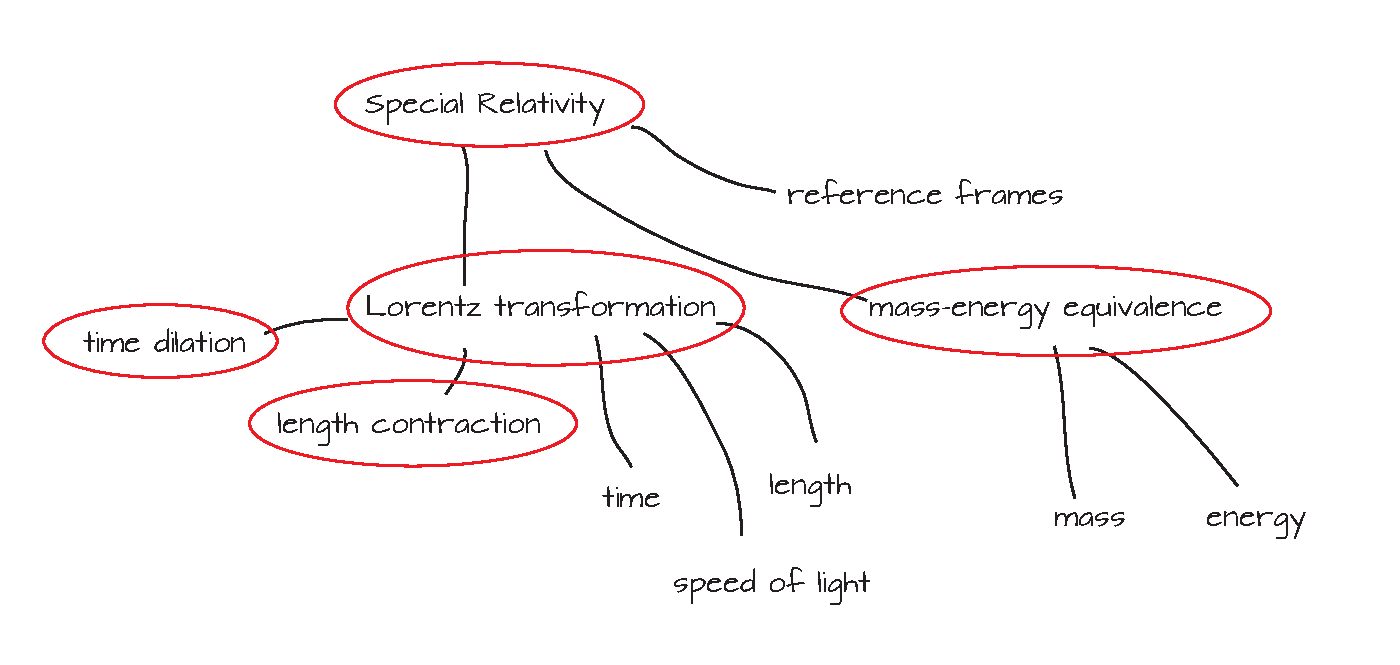
\includegraphics[width=0.75\textwidth]{FacesDay1/figs/ConceptBreakdown.pdf}
\captionof{figure}{If you were trying to break down special relativity, a \textit{portion} of your breakdown might look like this...}
\end{center}

Once you've done your breakdown, try to make the following lists individually:
\be
\item Relevant fundamental mathematical terms that I don't know
\item Relevant fundamental mathematical terms that I do know
\item Ideas specific to facial or image recognition that I don't know
\item Ideas specific to facial or image recognition that I do know
\ee

\pagebreak
\shipoutAnswer

\chapter{Night 4: Facial Recognition, Image Manipulation and Decomposition}

\begin{learningobjectives}
\emph{Concepts}
\bi
\item Describe how a vector can be used to represent a data set.
\item Explain how a matrix is used to represent multiple data sets.
\item Explain what is meant by vectorizing a grayscale image.
\item Predict the size of a vectorized image, given its pixel dimensions and color (gray or color). 

\ei
\emph{MATLAB skills}
\bi
\item Convert a color image into a grayscale image.
\item Convert an image to a matrix and back again
\ei
\end{learningobjectives}

\section{Ethics, Artificial Intelligence, and Facial Recognition}

Face recognition is a technology with many possible applications.  In just the past dozen or so years, the technology has gone from the stuff of science fiction to something that we interact with everyday (e.g., auto-tagging of images uploaded to social media).  In this part of the assignment we are going to ask you to take a deep dive into how this technology manifests itself in the real world---often with mixed consequences for society.

This section is structured into three parts.  First, we'll have you read about some of the issues that have been raised around face recognition technology (and more generally face analysis technology).  Next, you'll read some frameworks that have been proposed to help mitigate the potential harm and maximize the benefits that might otherwise come from releasing poorly tested and biased AI systems.  Finally, we'll have you branch out from face recognition technology to AI in general to examine which applications of the technology you think have the potential to most positively impact the world.  You will discuss and synthesize your findings in class on Thursday, so make sure to take some sort of notes on what you read (there are also some specific prompts to respond to below).

\subsection{Face Recognition Technology}


\begin{prob}
For a good overview of the issues, we'd like you to read \href{https://docs.house.gov/meetings/GO/GO00/20190522/109521/HHRG-116-GO00-Wstate-BuolamwiniJ-20190522.pdf}{Joy Buolamwini's written testimony} that she then \href{https://youtu.be/jLmzEFkbNsg?t=2910}{presented orally} .  You can pick whether you read the testimony or watch the video, although one nice thing about the written testimony is that it cites a lot of sources that you can read for more information.

\emph{Based on this reading, generate a list of surprising insights (e.g., spurred by key quotes) that you gained.  Also generate at least one discussion question.}
\end{prob}

\subsection{Frameworks and Guidelines for Responsible Machine Learning}

\begin{prob}
Face recognition technology falls under the umbrella of machine learning.  Machine learning is a field concerned with creating technologies that enable computers to learn to perform tasks automatically from experience (e.g., recognizing someone's identify from a picture of their face)---often by ingesting large training sets of labeled data.  Sparked by a recognition that machine learning technologies were causing unanticipated harm in the real world, a lot of attention has been paid in recent years (both in industry and academia) to issues of fairness, accountability, and transparency.  Here are two frameworks that have been created.
\begin{itemize}
\item \href{https://www.fatml.org/resources/principles-for-accountable-algorithms}{Principles for Accountable Algorithms}
\item \href{https://cloud.google.com/inclusive-ml/}{Google's Inclusive ML}
\end{itemize}

\emph{Based on this reading, generate a list of surprising insights (e.g., spurred by key quotes) that you gained.  Also generate at least one discussion question.}

To get a sense of all of the conversations taking place around this topic, check out \href{https://facctconference.org/network/}{ACM's FAccT network of events}.
\end{prob}

\subsection{Beyond Face Recognition}

One thing that is important to mention at this point in the module is that while we are learning linear algebra and data analysis techniques within the context of face recognition, what you are learning can be applied to innumerable applications and fields of study.  Even if we just stay within the realm of artificial intelligence, what you are learning now (and will learn later in the course) is the bedrock of many AI algorithms that are used in all sorts of applications.  When learning about all of the issues that a technology like face recognition has, we find that students can sometimes have a tendency to move towards a nihilistic perspective on technology as a whole (e.g., all technology is bad / harmful).  Critiquing technology and its role and effect in society is absolutely vital for \emph{any} engineer.  However, we contend that trying to understand how technology can be developed in a way that minimizes harm while maximizing benefit (e.g., the frameworks from the previous section) or by applying technology to problems or domains that have great potential for positive impact is also crucial.  In this section, we are asking you to look into applications of image analysis (or artificial intelligence more generally) that have the potential for great positive impact on society.

\begin{prob}
Find an article or paper about an application of artificial intelligence (it could be specifically about image or face analysis, but it need not be) that you think has the potential for great positive impact on society.  Come to class ready to summarize the application and why you think it has the potential for positive impact.  Unpack the notion of positive impact by specifying what the benefits (or downsides) would be of the application and who would reap them.

If you need some inspiration, here are some starting points (we are not claiming these are necessarily unambiguously positive, but they may provide some good starting points for your search).
\begin{itemize}
\item Automated diagnosis of cancer from medical images
\item Automated, personalized education
\item Optimizing energy use with artificial intelligence (more generally ``Computational Sustainability'')
\item Sensing for driverless cars (e.g., pedestrian detection, road sign reading)
\item Recognition and reading of text in a camera feed for people who are blind
\item Automated wildlife monitoring via image analysis
\item This one is kind of cheating. Olin 2nd year Austin Vesiliza put together \href{https://www.notion.so/ML-for-Good-c0cc352c88b04e719c187c8e4a6f5887}{a list of links to AI for social good projects} that you might use for inspiration.
\end{itemize}
\end{prob}

\section{Manipulating Images with Matrices}

\begin{center}
\includegraphics[width=0.75\textwidth]{FacesNight1/figs/RGBArrayWithSlice.pdf}
\captionof{figure}{Anatomy of an RGB image array.}
\label{fig:StackedRGBArray}
\label{fig:RGBArray}
\end{center}

\begin{prob}
    Our next example is of an image pre-processing step that many of you would eventually do using built-in MATLAB functions before running your face detection algorithm.
        \begin{enumerate}
        \item Read an image file using MATLAB, and convert it to double precision numbers (the data format that MATLAB uses by default for vectors and matrices) using the following code:
        \begin{verbatim}
        X = imread(`giraffe.jpg');
        \end{verbatim}
        (If you get an error, try re-typing the apostrophes.)

        \item Color images are stored in a 3-dimensional array (as opposed to matrices, which are 2-dimensional arrays) in MATLAB. Compare this to the smiley face image you saw in class which was a matrix whose entries are the gray-scale values. Here, instead of gray-scale values, the color information is stored in Red, Green and Blue entries of the three-dimensional array. Therefore, each pixel in the image is associated with three different values which indicate how much of Red, Green and Blue are present in that pixel.  This array is illustrated in Figure \ref{fig:RGBArray}.

         You can see the dimensions of this array using the following.
        \begin{verbatim}
        size(X)
        \end{verbatim}

        \item Display the image using

        \begin{verbatim}
        imagesc(X);
        \end{verbatim}

    The image may be squashed; if you would like it not be be squashed, type \texttt{axis equal} into the command window.

    \item What will the dimensions of the matrix with the grayscale representation of this image be? 
    
    \item We will now use matrix manipulations to turn the image into a grayscale image. The RGB array can be separated into three slices, one for each color. For example, the red slice is all the data in the the first layer of the array:
    \begin{verbatim}
    X_red=X(:,:,1);
    \end{verbatim}

    Converting a pixel to grayscale can be accomplished by taking a linear combination of the red, green and blue values of that pixel which are weighted by 0.2989, 0.5870 and 0.1140 respectively. Use these weights to create a linear combination of the red, green, and blue slices.


    \item  Verify if this was done correctly by displaying the image using the following commands.
    \begin{verbatim}
    imagesc(grayscaleX); colormap('gray'); axis equal
    \end{verbatim}

    \end{enumerate}
    \end{prob}
    
    \begin{sol}
    \begin{enumerate}
    \item 
        \item The size of the array is $740\times740\times3$.
        \item You should see the following picture:
            \begin{center}
            \includegraphics[scale=.4]{FacesNight1/figs/giraffe.jpg}
            \captionof{figure}{Giraffe}
            \label{fig:giraffe}
            \end{center}
        \item The gray-scale version of this image is represented by a $740\times740$ matrix.
        \item Create the matrix $\mathbf{grayscaleX}$ which represents the grayscale version of this image using \texttt{>> grayscaleX = 0.2989*X(:,:,1) + 0.5870*X(:,:,2) + 0.1140*X(:,:,3)}.
        \item You should see the following image:
                \begin{center} \includegraphics[scale=.4]{FacesNight1/figs/graygiraffe.jpg}
                \captionof{figure}{Gray Giraffe}
                \label{fig:graygiraffe}
                \end{center}
    \end{enumerate}
    \end{sol}

\section{Further Examples on Decomposition}


\begin{prob}
\begin{enumerate}

\item In this problem, we are going to express the temperature data for four cities we encountered earlier using a given set of basis vectors. Load some sample temperature data in MATLAB by typing \texttt{>> load  temperatures\_and\_bases.mat}. Type \texttt{whos} at the MATLAB prompt to see all your variables. You should have a matrix \texttt{T} which has the temperature data for 1 year for the cities of Boston, New York, Washington DC and Providence in that order. Use the \texttt{size} command to determine how the data are organized in this matrix. You should also have four vectors $\u_1\cdots\u_4$ which a genie has provided to you.

\begin{enumerate}

\item Verify that the vectors $\u_1, \cdots \u_4$ are all mutually orthogonal, and that they have unit length.

\item Set up and solve the linear algebra problem in order to express each column of the temperature matrix \texttt{T} as a linear combination of $\u_1\cdots\u_4$. Check that you can undo this operation and retrieve the original data.

\item Now let's reconstruct an approximation to the original temperature data, using only the vectors $\u_1, \u_2, \u_3$, What is the rms error for this approximation?

\item Compare the rms error for the previous scheme to a simpler scheme where in order to compress the data, we simply discard the temperature of Providence. When we want to reconstruct the data, we simply approximate the temperature in Providence by the temperature in Boston.

\end{enumerate}

Once again, we have to disappoint you by letting you know that there is no genie! There is just data. In the coming weeks, we are going to find out how to find bases vectors that can be useful for dimensionality reduction for a given set of random data, given some training data. This will be particularly useful in speeding up computations where instead of doing computations on all the dimensions of the data we have, we perform computations on fewer dimensions.

\item We will finally be dealing with images of faces. We are going to compress these face images in a similar way as the temperature data (we give you the bases). Here, the data have really high dimensions (each pixel is a dimension). The bases that we give you (matrix $\mathbf{U}$) doesn't span the entire high dimensional space (so there will be lossy compression).

\begin{enumerate}

\item Load the file \texttt{face\_bases.mat} in MATLAB. You will see a 3-dimensional array \texttt{test\_images}, of dimensions $256\times 256\times 424$, and a matrix \texttt{U} of dimensions $65536 \times 424$. The \texttt{test\_images} array contains 424 grayscale images.Each image is $256 \times 256$ pixels.

\item Select any one image from the set of 424 and call it \texttt{T}. Display this image using \texttt{>> imagesc(T); colormap('gray')}. This image is currently represented as a $256 \times 256$ matrix of grayscale values. We will find it very convenient to work with vectors instead of matrices representing an image. Therefore, to make our lives simple, we will take the data for an image which is stored in a matrix and store it in a vector.

We are going to \emph{vectorize} this image by stacking its columns one on top of another to create a single vector that is $(256)^2 \times 1$, i.e. $65536 \times 1$ which will be a lot easier to work with. This operation can be accomplished in MATLAB as follows: \texttt{>> Tstacked = reshape(T, 65536,1);}. When you need to recover the unstacked version of the image, you can undo-the stacking as follows: \texttt{>> Tunstacked = reshape(Tstacked, 256, 256)}.

\item The matrix \texttt{U} contains a set of 424 $65536 \times 1$ linearly independent vectors provided by the genie. Approximate the \texttt{Tstacked} vector as a linear combination of the first $10$ of columns of \texttt{U}, and call this vector \texttt{Tapprox10}. \texttt{Tapprox10} should be a 65536 $\times$ 1 vector, and you will only have 10 weight values to find this approximation. See how well this approximation works by reshaping \texttt{Tapprox10} into a $256 \times 256$ matrix and displaying it using \texttt{imagesc} and \texttt{colormap('gray')}.

\item Now repeat the previous exercise with the first 50 columns of \texttt{U} and then again with the first 100 columns of \texttt{U}. 

\end{enumerate}

You should observe that the more columns of \texttt{U} you use, the better the approximation. Note here that we are trying to approximate a 65536 dimensional vector using 10, 50 and 100 numbers. Therefore, you should not expect the approximation to work super well, but with 100 columns of \texttt{U}, you should be able to recognize the picture. At a later date we will quantify the fidelity of the approximation.

Note that more sophisticated image compression algorithms use methods that rely on special properties of images and human vision in order to a achieve high degree of compression.

\end{enumerate}
\end{prob}
\begin{sol}
\begin{enumerate}
    \item \begin{enumerate}
        \item To check that \texttt{u1} and \texttt{u2} are orthogonal, type \texttt{>> transpose(u1)*u2}. The result should be zero. Check the other five pairs of vectors.
        
        To check that \texttt{u1} has unit length, type \texttt{>> transpose(u1)*u1}. The result should be one. Check the other three vectors.
        
        \item First we need to construct a matrix \texttt{U} with columns each of the $\mathbf{u}_i$\\
        \texttt{>> U=[u1 u2 u3 u4],}\\
        and convert \texttt{T} to the basis of $\mathbf{u}_i$ vectors by multiplying
        \texttt{>> Tu=U*T.} You can recover the original data with \texttt{>> inv(U)*Tu}.
        
        \item 
        \item
    \end{enumerate}
    \item \begin{enumerate}
        \item 
        \item
        \item Isolate the first 10 columns of \texttt{U} using \texttt{>> U10=U(:,1:10);}. Then determine the weights for each of these column vectors using\\
        \texttt{>> Tweights10=transpose(Tstacked)*U10;}\\
        and then take the linear combination\\
        \texttt{>> Tapprox10=U10*transpose(Tweights10);.}
        Then we unstack the vector into a matrix\\
        \texttt{>> Tapprox10unstacked=reshape(Tapprox10,256,256);}
        and display the image.
        \item 
    \end{enumerate}
\end{enumerate}
\end{sol}

% \subsection{Check in with your concept map}

% \begin{prob}

% Pull up the picture of your concept map of eigenfaces from the first day of this module.  Annotate this picture (in whatever way you prefer) to indicate where we have gotten so far in this.  Add additional bubbles or nodes to the concept map if there are things we have learned up to this point that were not in your original!  Also annotate your concept map as to which things we still need to learn to get all the way to eigenfaces.

% \end{prob}

\section{Data: Many Measurements of the Same Thing}
{One of the simplest forms of data} is a set of data which represents many measurements of nominally the same thing.  Depending on what the goal is of our analysis, this might encompass measurements of the same quantity across many different situations, or many instances of the same situation.
\subsection{Visualizing Measurements of the Same Thing}

It's usually a good idea to \textit{look} at data before you start calculating things associated with it.

You've surely encountered these ideas before, but for the sake of completeness, we'll highlight a couple of ideas here.  If you have a large number of data points (say, for example, that you measured the heights of a bunch of different people), you might choose to simply plot the data versus the person number -- the index.  Note here that the data is plotted as individual points, since each point represents a measurement.  Ideally we might also include error bars here to indicate our uncertainty in a given measurement, but for now, let's leave that out.

\begin{center}
\includegraphics[width=0.75\textwidth]{FacesNight3/figs/singlevariableplot.jpg}
\captionof{figure}{An example of a single variable plot}
\label{fig:single-var-plot}
\end{center}

Alternatively, you could also visualize many measurements of the same thing by creating a \textit{histogram}.  This is a representation of how many measurements fall into different ``bins'': the height of a given bar is the number of samples that fall within the range associated with the bar.  For example, in the figure, you can see that about 20 million people made between 0 and \$5000 in 2008.  You've likely seen this kind of thing before as well: it's not an uncommon way to represent test scores.

\begin{center}
\includegraphics[width=0.75\textwidth]{FacesNight3/figs/incomehistogram.png}
\captionof{figure}{An example of a histogram.}
\label{fig:histogram}
\end{center}

Note, of course, that how a histogram \textit{looks} depends on what you choose for the bins - both how many there are, and where they are centered!

\subsection{Common Figures of Merit for the Same Thing }
While looking at the data is certainly helpful, we can also extract or calculate a couple of important figures of merit of the data.  The first is the average, or \textit{mean} of the data, given by summing all the elements in the dataset $\{d_i\}$ and dividing by the number $N$ of elements in the set:
\begin{equation}
\mu  =  \frac{1}{N}\sum_{i=1}^N d_i
\end{equation}
Note that if our data is a continuous function $f(x)$ over a range of the independent variable $x$ as opposed to a set of discrete points, we can express the same thing as an integral:
\begin{equation}
\mu = \frac{\int_{range} f(x) dx}{\int_{range} dx}
\end{equation}
The average captures the center or 'expected value' of the distribution of data.  In addition to this, it is often helpful to capture the spread of the data around this average.  There are a few different metrics which are used for this.  A simple one is the \textit{variance} from the mean, $\sigma^2$:  the average of the squared difference between each data point and the mean.
 \begin{equation}
\sigma^2  =  \frac{1}{N-1}\sum_{i=1}^N (d_i - \mu)^2
\end{equation}
Please note that this definition normalizes using $N-1$, but you will often see alternative definitions which normalize using $N$. Another commonly encountered measure is the \textit{standard deviation}, which is simply the square root of the variance from the mean:
 \begin{equation}
\sigma  =  \sqrt{\frac{1}{N-1}\sum_{i=1}^N (d_i - \mu)^2}
\end{equation}

\begin{prob}
\begin{enumerate}
\item Look at the single variable plot in Figure~\ref{fig:single-var-plot} above.  Estimate the value of the mean and the value of the standard deviation.  What are the units of each?
\item Look at the histogram plot in Figure~\ref{fig:histogram} above.  Estimate the value of the mean and the value of the standard deviation.
\item What is the mean and standard deviation of this data set (Do this in your head!)
$$\{1,3,1,3,1,3,1,3,1,3,1,3,1,3,1,3,1,3,1,3\}$$
\item  Begin by considering the simple dataset of the high temperatures in Needham for ten days in March:
\begin{equation}
T = \{57,61,46,43,46,46,54,46,46,55\}
\end{equation}
\begin{enumerate}
\item  By hand, create a histogram of this data.  What size bin makes sense? What bin centering makes sense?
\item  By hand, compute the mean temperature over these ten days.  If you look at the data, does this mean make sense?
\item  By hand, compute the variance and standard deviation of the temperature over these ten days.  If you look at the data histogram does this make sense?
\item  This dataset has a flaw: it has a small number of datapoints.  What do you see as the possible effects of having such a small sample?
\end{enumerate}
\item  Now consider the larger dataset below of the approximated heights of the Olin faculty, measured in inches.  In MATLAB, create a vector which has this dataset as the entries.
\begin{align*}
H = &\{63,66,71,65,70,66,67,65,67,74,64,75,68,67,70,73,66,70,72,62,68,\\
&70,62,69,66,70,70,68,69,70,71,65,64,71,64,78,69,70,65,66,72,64\}
\end{align*}
\begin{enumerate}
\item  Computationally histogram this data.  What size bin makes sense?  What bin centering makes sense? Try a few different combinations. See MATLAB function \texttt{histogram}.
\item  Computationally, find the mean, standard deviation, and variance of this dataset. See MATLAB functions \texttt{mean}, \texttt{std}, and \texttt{var}.
\item  Does the mean, standard deviation, and variance make sense given the histogram of the data?
\end{enumerate}
\end{enumerate}
\end{prob}
\begin{sol}
\begin{enumerate}
    \item Assuming that the ``heights'' plotted are heights of randomly selected humans, then the unit for the mean and standard deviation is inches.
    \item 
    \item Since half the digits are 1 and the other half are 3, the mean will be the average of 1 and 3, so $\mu=2$. Looking at the formula for standard deviation, we can see that $d_i-\mu = 1$ for each data point, so $\sigma = \sqrt{20/19}$.
    \item \begin{enumerate}
        \item 
        \item We compute $\mu=50$.
        \item We compute $\sigma=6.15$.
        \item 
    \end{enumerate}
    \item 
    \begin{enumerate}
        \item By simply entering \texttt{>> histogram(H)}, MATLAB automatically chooses bins of size one.
    \item Using MATLAB we find that $\mu = 68.1429$, $\sigma = 3.5721$ and $\sigma^2 = 12.7596$.
    \item 
    \end{enumerate}
\end{enumerate}
\end{sol}


\section{Brightness and Contrast}
The brightness and contrast of images is controlled by scaling the histogram of the pixel values.  Try this out!

Note:  for displaying images in this part, make sure to NOT use imagesc:  imagesc is specifically setup to auto-scale the image to use the full range from 0 to 255. Just use the command `image'.

\begin{prob}
    \begin{enumerate}
    \item  Load an image of your choice into MATLAB using the \texttt{imread} command.  (Make sure you are in the correct directory for the image or give it the complete path). Display the image using the `image' command.
    \item  If your image is a color image, convert it into grayscale by using the \texttt{rgb2gray} command.
    \item  Create a vector of the intensities in your image: use the \texttt{reshape} command to create a giant column vector in which the first $n$ elements are the first column of the image, the next $n$ are the second column, etc.
    \item Make a histogram of the intensity values in your image.  Note that the default variable type for image data is uint8 (8-bit unsigned integer) which is an integer that ranges from 0 to 255.   Does your image use the entire range of values from 0 to 255?  What is the minimum pixel value used?  What is the maximum?
    \item  Find the mean of the intensities in your image data.  Find the standard deviation.  Is the intensity data well-centered on the available range?  The location of the intensity data in the range determines the brightness of the image. How does the standard deviation compare to the available range?  Does the intensity data span a good portion of the available range? This affects the contrast.
    \item  To adjust the brightness of your image, you can scale all of the intensity values by a multiplicative factor down (towards darker values) or up (towards brighter values).  Based on looking at the histogram, should your image be brightened?  Dimmed?  Why?
 \item To adjust the contrast, you make a linear mapping of the existing range onto the full 0 to 255 range.  In other words, if you think of the current intensity value as your independent variable $x$, and the new intensity value as the dependent variable $y$, a contrast adjustment is defined by a function $y = f(x)$.  Propose an equation for a line which gives you the ``best'' range of y's, given the input intensity values in the image.  You should be able to justify this based on the histogram of the image.  Note that any values  of $y$ that end up below 0 should be interpreted as 0, and any values over $255$ should be interpreted as $255$.
 \item Implement brightness and contrast adjustment:
 \begin{enumerate}
 \item Load a picture of a face.
 \item Analyze the intensity histogram.
 \item Calculate the adjusted face by applying both brightness and contrast adjustments to make it as ``good'' as possible.
 \item Create a figure that includes four subplots: the original image, the original intensity histogram, the new image, and the new intensity histogram.
 \end{enumerate}
 \item What would happen if the function for contrast adjustment was not linear?  Why might you choose a non-linear function for this mapping?
 \end{enumerate}
\end{prob}

\pagebreak
\shipoutAnswer

\chapter{Day 5: LSAE, Brain data, and C\&E}

\section{Schedule}
\begin{itemize}
    \item 0900-0915: Table Dynamics Discussion
    \item 0915-1010: Debrief and Synthesis
    \item 1010-1025: Coffee Break
    \item 1025-1035: Correlation
    \item 1035-1135: Brain Data with Samantha Michalka!
    \item 1135-1220: AI and Society Discussion
    \item 1220-1230: Day Survey
\end{itemize}

\section{Table Dynamics Survey Discussion}

\section{Debrief and Synthesis}

\bi
\item Please discuss your overnight work with your table-mates, and get help with the ideas that you are still confused by.
\ei

In the next set of exercises we will explore a common method for finding ``the'' solution of a linear system of algebraic equations $(\A \x = \b$) in the case where there are more equations that unknowns (more rows than columns). We will first need to synthesise some previous ideas about the span of vectors.

\subsection{Range of $\A$}

We discussed earlier the concept of the \textbf{span} of a collection of vectors. Recall that the span of a collection of vectors is the set of all linear combinations of the vectors. Now we will apply this concept to the columns of a matrix:

\begin{quote}
Definition: The Range of a matrix $\A$ is the span of its columns. 
\end{quote}

\begin{prob}
Describe in words the Range of the following matrices:
\be 
\item $\A = \twobyone{1}{1}$
\item $\A = \threebytwo{1}{2}{1}{3}{0}{0}$
\item $\A = \threebytwo{1}{2}{3}{4}{5}{6}$
\ee
\end{prob}

\begin{sol}
\be
\item The column is a two-dimensional vector. The span is a line (slope = 1) in 2D space. 
\item The columns are linearly-independent three-dimensional vectors. Their span is therefore a plane in 3D space. Since all the z-entries are zero, the plane is actually the xy-plane.
\item The columns are linearly-independent three-dimensional vectors. Their span is therefore a plane in 3D space. The plane is defined by the column vectors.
\ee
\end{sol}

\subsection{Exact Solution to $\A \x = \b$}

When does a linear system of algebraic equations, $\A \x = \b$, have a solution? Since the product $\A \x$ is a linear combination of the columns of $\A$, then $\A \x = \b$ will have a solution if and only if $\b$ is in the Range of $\A$. Think about that, and complete the following exercise.

\begin{prob}
Which of the following linear systems of algebraic equations will have a solution? Think about it from an equation perspective and the Range of $\A$ perspective.
\be
\item $\A = \twobyone{1}{1}$ and $\b = \twobyone{5}{5}$ 
\item $\A = \twobyone{1}{1}$ and $\b = \twobyone{2}{3}$
\item $\A = \threebytwo{1}{2}{3}{4}{5}{6}$ and $\b = \threebyone{3}{7}{11}$
\item $\A = \threebytwo{1}{2}{3}{4}{5}{6}$ and $\b = \threebyone{3}{7}{5}$
\ee
\end{prob}
\begin{sol}
\be
\item The Range of $\A$ is all multiples of $\twobyone{1}{1}$. Since $\b$ is a multiple of this vector then there is a solution. From an equation point of view, the solution is simply $x=5$.
\item The Range of $\A$ is all multiples of $\twobyone{1}{1}$. Since $\b$ is not a multiple of this vector then there is no solution. From an equation point of view this makes sense because we are demanding that $x=2$ and $x=3$ at the same time.
\item The Range of $\A$ is a plane in 3D. Since $\b$ is the sum of the columns it must be in the Range of $\A$ and so there is a solution. From an equation point of view there are two linearly-independent equations in two unknowns.
\item The Range of $\A$ is a plane in 3D. Since $\b$ is not in this plane there is no solution. From an equation point of view this makes sense because trying to solve the equations results in an inconsistency.
\ee
\end{sol}

\subsection{Approximate solution to $\A \x = \b$}
You should have found that some of these systems do not have a solution in the usual sense, i.e. there is no vector $\x$ which makes the equation $\A \x = \b$ true. We might refer to such a solution as an \textbf{exact} solution. We will now consider an \textbf{approximate} solution, i.e. a vector $\x$ which approximately satisfies $\A \x = \b$. We will consider a particular approximation based on \textbf{orthogonal projection} now, and later in this module we will look at this approximation from a different perspective where it is known as the \textbf{Least-Squares} approximation. We met orthogonal projection earlier in the module when we spoke about vector components and basis vectors.

\begin{prob}
Hold your hand up in front of you, and think about it as occupying a location in 3D.
\be
\item Point to the location on the front wall that is closest to your hand.
\item Point to the location on the floor that is closest to your hand.
\item Have one of your table-mates hold a mobile white board at some angle. Now point to the location on the white board that is closest to your hand (you might have to imagine a larger mobile white board).
\item What is the relationship between the ``pointing'' vector and the surface being pointed at?
\ee
\end{prob}
\begin{sol}
In each case the ``closest'' point is the location where the ``pointing'' vector meets the surface at right angles, i.e. they are orthogonal.
\end{sol}

Now let's put this in the context of solving $\A \x = \b$. 

\bi
\item If $\b$ is not in the Range of $\A$ then we will define an approximate solution by orthogonal projection of $\b$ onto the Range of $\A$. 
\item The ``pointing'' vector from $\b$ to the relevant point in the Range of $\A$ is $\A \x - \b$. 
\item Since the Range of $\A$ is defined by the span of the columns of $\A$ then the ``pointing'' vector must be orthogonal to \textbf{every} column of $\A$. 
\item This implies that $\A^T (\A \x - \b) = \mathbf{0}$. (Think about why this must be true). 
\item Re-arranging this equation leads to $\A^T \A \x = \A^T \b$. The matrix $\A^T \A$ is a square matrix (which we will meet again and again this module). 
\item This is a linear system with equal numbers of equations and unknowns and can therefore be solved using our usual techniques. Did you get that? You should re-read this paragraph a few times. To summarize:
\ei

\begin{quote}
The approximate solution to $\A \x = \b$ based on orthogonal projection can be obtained by solving
\[\A^T \A \x = \A^T \b \]
This solution is also known as the \textbf{least-squares} solution because it minimises the distance between $\b$ and the Range of $\A$ (more about this later in the module).
\end{quote}

\begin{quote}
\textbf{Warning:} Do not think about $\x$ defining a coordinate system that $\b$ lives in! When you draw a picture you should think about the space that the columns of $\A$ live in. We are projecting $\b$ onto a basis defined by the columns of $\A$. The solution vector $\x$ is better thought of as a set of ``weights'' or ``coordinates'' with respect to this basis.
\end{quote}

\begin{prob}
\be
\item Consider the linear system $\A \x = \b$ where $\A = \twobyone{1}{1}$ and $\b = \twobyone{2}{3}$. (You've already thought about this earlier). 
\be
\item Sketch the Range of $\A$ and locate the point in the Range that is closest to $\b$.
\item Multiply both sides of $\A \x = \b$ by $\A^T$ and solve the resulting linear system.
\ee
\item Consider the linear system $\A \x = \b$ where $\A = \threebytwo{1}{2}{3}{4}{5}{6}$ and $\b = \threebyone{3}{7}{5}$. (You've already thought about this earlier). 
\be
\item Sketch the Range of $\A$ and locate the point in the Range that is closest to $\b$.
\item Multiply both sides of $\A \x = \b$ by $\A^T$ and solve the resulting linear system.
\ee
\ee
\end{prob}
\begin{sol}
\be
\item Consider the linear system $\A \x = \b$ where $\A = \twobyone{1}{1}$ and $\b = \twobyone{2}{3}$. (You've already thought about this earlier). 
\be
\item Sketch the Range of $\A$ and locate the point in the Range that is closest to $\b$. (The Range is a straight line and the point is the orthogonal projection onto this line.)
\item Multiply both sides of $\A \x = \b$ by $\A^T$ and solve the resulting linear system. (You should find that $x = 5/2$).
\ee
\item Consider the linear system $\A \x = \b$ where $\A = \threebytwo{1}{2}{3}{4}{5}{6}$ and $\b = \threebyone{3}{7}{5}$. (You've already thought about this earlier). 
\be
\item Sketch the Range of $\A$ and locate the point in the Range that is closest to $\b$. (The Range is a plane in 3D and the point is the orthogonal projection onto this line.)
\item Multiply both sides of $\A \x = \b$ by $\A^T$ and solve the resulting linear system. (You should find that $x=-3$ and $y=7/2$.)
\ee
\ee
\end{sol}
\subsection{Solving $\A \x = \b$ in Matlab}

In many ways Matlab makes life easy for us. There is a single command in order to solve a linear system $\A \x = \b$
\begin{verbatim}
>> x = A\b
\end{verbatim}
although it can also be used by typing
\begin{verbatim}
>> x = mldivide(A,b)
\end{verbatim}
If there are more rows than columns then Matlab finds the approximate solution we discussed above. If there are equal numbers of rows and columns then Matlab computes a solution by LU decomposition. If there are less rows than columns then Matlab computes one of the infinite number of solutions - the solution it computes is not an approximation but it does select the solution that minimizes the length of the solution vector.

\section{Correlation (activity sheet will be printed available at your table)}

\section{Analyzing brain data with special guest star Sam Michalka!}

In this section, you are going to find the correlation between 12 brain regions and use this to support the hypothesis that these regions are part of two different ``networks.'' Brain regions are considered to be part of a network if the signals in the regions are correlated with each other. Here, we are going to look at the correlations of really slow changes over time (several seconds).

We have already collected the data using functional magnetic resonance imaging (fMRI), which looks at changes in the amount of oxygen in the blood in the brain. These changes in oxygen levels are related to large populations of neurons firing and changes slowly and with several seconds of delay.  Here, we are going to refer to the signal that the fMRI detects as ``activity'' in the brain (this is a gross oversimplification of what's going on, but is enough to approach this analysis with some guidance.  Feed Sam coffee if you want to know more.)

\begin{center}
\includegraphics[width=0.75\textwidth]{FacesDay4/figs/brainimages.pdf}
\end{center}

The fundamental idea behind what we are looking for is as follows:
\begin{itemize}
\item The brain can be divided into different regions (physical areas of the brain that are thought to serve some shared purpose). The brain is approximately symmetrical and has a left and a right hemisphere.
\item We have identified 12 brain regions to investigate: 6 in the left hemisphere and 6 in the right hemisphere. They all have long fancy names (such as left superior precentral sulcus) and abbreviations (Left\_sPCS). Due to the symmetry of the brain, there are matching names in each hemisphere (Right\_sPCS and Left\_sPCS both exist).
\item The 12 brain regions that were selected were chosen because a previous experiment indicated that these regions are part of two different networks: one network that is more involved in processing auditory (sound) information and one network that is more involved in processing visual information.
\item Our goal is to look at the correlation between the activity in each of these regions and the other 11 regions. Based on our first study, we hypothesize that the regions in blue will be correlated with other regions in blue to form a ``visual network'' and the regions in orange will be correlated with other regions in orange to form an ``auditory network''.
\end{itemize}
We have given you the data from one person (the actual study had more people). Also, we are not going to worry about statistical testing here; we are just going to look at the correlations in relation to each other.

\begin{center}
\includegraphics[width=0.75\textwidth]{FacesDay4/figs/brainrpaud80.png}
\end{center}

Let's analyze some brain data! The plot below shows the first 80-ish seconds of data from the ``right posterior auditory region'' or ``Right\_pAud''.

\begin{prob}
\begin{enumerate}
\item \textbf{Consider your data and hypothesis.} Before you transform into a Matlab-mastermind, let's take a minute to think and work on the whiteboard.
\begin{enumerate}
\item Roughly sketch a signal like the one shown in the plot above and label it ``A''.  Don't worry about the details of this signal, just draw some bumps at approximately the same places.
\item Sketch a line for a signal that has a high (but not perfect) positive correlation with ``A''. Label it ``B''. (A different color for each signal would be nice, if convenient.)
\item Sketch a line for a signal that has a high (but not perfect) negative correlation with ``A''. Label it ``C''.
\item Sketch a line for a signal that is uncorrelated with ``A''. Label it ``D''.
\item Make a rough estimate of the correlation between each of these pairs of signals. Organize these estimates in a 4 x 4 table and add labels.
\item Discuss alternate signals that you could have drawn for B, C, and/or D.
\end{enumerate}

\item \textbf{Load and explore the data.} Whenever you encounter a new data set, it's helpful to look at the variables and make a few quick plots.
\begin{enumerate}
	\item Load the fmridata.mat file.
	\item Make sure you have the proper variables.
	\begin{itemize}
		\item There should be 12 brain region vectors, each starting with the word ``Left'' or ``Right'' (e.g., \texttt{Left\_sPCS}). Each value in the vector contains a measurement at a particular point in time. The data were collected for a period of 11 minutes and 5.6 seconds. Measurements were taken every 2.6 seconds.  A timepoint refers to one of those 2.6 second increments. How many timepoints do you expect? Does this match your vector length?
		\item The variable \texttt{braindata} contains all 12 brain region vectors organized into an array with dimensions \texttt{timepoints} $\times$ \texttt{brain regions}.
		\item The variable \texttt{names} contains the names of the 12 brain regions in an order that matches \texttt{braindata}.
		% Validate this by plotting the vector for a random region using the vector variable and by using braindata. These should be identical.
		\item The variable \texttt{uncleandata} is similar to \texttt{braindata} and can be ignored for now.
\end{itemize}

	\item Generate a plot with time on the x-axis and ``activity'' (the data values) on the y-axis. Represent each brain region as a line. You will first need to generate a new vector called \texttt{time} that represents the appropriate time increments (see above). Do your data seem reasonable? How do you know?
	
%	\item Create a separate histogram for each brain region. [Note: you can use \textit{subplot(3,4,plotnumber)} and a \textit{for loop} to generate these histograms without making 12 individual figures.

%	\item What do you observe from this plotting? Do your data seem reasonable? How do you know?
\end{enumerate}


\item \textbf{Focus on a few pairs of regions.} The plot of all brain regions over all time points had a lot of information, so let's zoom in a bit and tie things back to the question at hand. Are the ``auditory'' (orange) regions correlated with other ``auditory'' regions? And are they correlated with the ``visual'' (blue) regions?  Let's use one ``auditory'' regions called \texttt{Left\_pAud} to investigate. The region \texttt{Left\_pAud} is in the left hemisphere of the brain and should be colored orange in the image of the brains above.

\begin{enumerate}
\item Let's begin looking the relationship between \texttt{Left\_pAud} and \texttt{Right\_pAud}.
\item Look at the brain image to determine if \texttt{Right\_pAud} is an ``auditory'' (orange) or ``visual'' (navy blue) type of region. Do you expect the activity of this region to be correlated with \texttt{Left\_pAud}?
\item Plot the signals from these two regions (with time on the x-axis). You may want to zoom in to the first 100 seconds to get another view. Guess the correlation between these regions.
\item Calculate the correlation between between the two regions using the built-in MATLAB function \texttt{corr} (remember, you can get more information on a MATLAB command by typing, for example \texttt{doc corr} or \texttt{help corr} into the MATLAB command prompt).
\item Is this correlation what you expected? How does it fit into our investigation of the correlation between ``auditory'' and ``visual'' regions?

\item Repeat the steps above to look at the relationship between \texttt{Left\_pAud} and \texttt{Left\_sPCS}.
\item Repeat the steps above to look at the relationship between \texttt{Left\_pAud} and \texttt{Left\_tgPCS}.

\end{enumerate}

\item \textbf{Bonus fun: Generalize your analysis to calculate and display the correlations between all pairs of brain regions.} We looked at a few specific pairs of brain regions, but now we want to investigate our hypothesis by looking at all possible pairs of brain regions.
\begin{enumerate}
\item Create a matrix that contains the values of the correlation between each brain region. This is the same idea as the table of correlations that you wrote on the board. (Hint: Use the \texttt{braindata} matrix instead of the individual brain region vectors.) You can confirm that your values are correct by comparing to the correlations that you calculated above.
\item Display this matrix using \texttt{imagesc}. The following code may be helpful in labeling the plot:
\begin{verbatim}
>> colorbar; colormap('jet'); caxis([-1 1]); 
% Set color bar parameters
>> xticks(1:12); xtickangle(-45); xticklabels(names); 
% Label x axis
>> yticks(1:12); yticklabels(names); 
% Label y axis
\end{verbatim}
\item Discuss your observations from this plot. Refer to the figure with the brain image to determine which brain regions are ``auditory'' regions and which are ``visual'' regions? What patterns to you observe about their correlations?
\end{enumerate}


\item \textbf{More Bonus fun: Explore the effects of preprocessing and outliers.} If you have extra time, check out the data in \textit{uncleandata}. This data has the same structure as \textit{braindata}, but contains some ``bad'' time points (208, 209, 210 , 232) caused by a blip in the recording equipment (this is a real problem that people face, though this example is extreme).

\begin{enumerate}
	\item Plot this data versus time. How does this compare to the ``clean'' data from \texttt{braindata}?
	\item Using the \texttt{uncleandata}, recreate the correlation matrix figure that you created using imagesc(), which shows the correlations between each pair of regions.  How does this compare to your original version of this figure? What is important about these differences?
	\item Try to clean the data yourself. There are many possible ways to deal with these ``bad'' timepoints, so you can choose one to investigate. Some options:
	\begin{itemize}
	\item Remove the timepoints completely.
	\item Replace the values at these time points with the mean of the good timepoints.
	\item Replace the values at these time points with a randomly selected value from the good timepoints.
	\item Another strategy of your choosing.
	\end{itemize}
\item Explain which strategy you chose and why. These are decisions that scientists and engineers have to make. There are pros and cons of each. It's really important to consider these and document the analysis decisions that you make.	
\item Discuss with your partner/table or reflect on your own: what are some of the potential ethical implications of "cleaning" data?

\item Plot the activity in all of the brain regions over time for your ``cleaned'' data.
\item Plot the correlation matrix figure for your ``cleaned'' data.
\item What similarities and differences do you observe between the correlation matrix for the ``unclean'' and ``clean'' data? How do you interpret these differences? What do you take away from this for future work?
\end{enumerate}
\end{enumerate}
\end{prob}

\section{AI and Society Discussion}

\subsection{Framing (5 minutes)}

Today we'll be talking about a constellation of issues that arise when AI technology, like facial recognition, is deployed in society.  As the historian Melvin Kranzberg famously remarked, ``Technology is neither good nor bad; nor is it neutral.''  As you saw in the reading from the night assignment, the effect of AI technology in society intersects a number of sensitive issues around race, class, and gender.  Due to intersection of AI and these sensitive issues, it helps to take a few minutes to consider some guidelines for having fruitful discussions at your tables.

\begin{itemize}
\item Check out \href{https://drive.google.com/file/d/1RZ9VHbWvsJwDbyF6zrmkd5mUdINrzt_f/view}{this poster} put together by some Oliners with suggestions for having conversations on sensitive topics.
\item The readings provide common information and framing, which we find is very helpful to finding common ground when discussing issues that individuals may relate to in very different ways.
\item As you may be relatively new to these ideas, consider adopting a mindset of identifying key questions rather than necessarily coming to conclusions.
\item When talking about the effect of a technology on a group that has been historically oppressed, you should be particularly sensitive in these discussions if you are not a member of this group.  Be conscious of the ways in which your words might be experienced by those who may have faced a history of discrimination due to being a member of this group.
\end{itemize}

\subsection{Unpacking the Readings (15 minutes)}
Write down key concepts and clear up points of confusion on the readings.

\begin{itemize}
\item \href{https://docs.house.gov/meetings/GO/GO00/20190522/109521/HHRG-116-GO00-Wstate-BuolamwiniJ-20190522.pdf}{Joy Buolamwini's written testimony} on bias in facial recognition technology (you may have watched this instead).
\item \href{https://www.fatml.org/resources/principles-for-accountable-algorithms}{Principles for Accountable Algorithms}
\item \href{https://cloud.google.com/inclusive-ml/}{Google's Inclusive ML}
\end{itemize}

\subsection{Share Your Positive Application of AI (10 minutes)}
Go around and share the application of AI that you think has the potential for great positive impact on society. Say a little bit about what you learned and how you think it would have a positive impact (e.g., in what ways and for whom).

\subsection{What Did You Take Away? (15 minutes)}

\textbf{Please have one person take notes on this in some electronic format so they can submit it as part of their day survey}

As a table, discuss what you took away from the readings and your discussion thus far.  Here are some dimensions that you might want to explore.
\begin{enumerate}
\item What parts or quotes from the readings were most surprising / impactful to you?
\item Were you surprised by your reaction to reading any of the material (e.g., felt unexpectedly angry, sad, indifferent)?
\item What are the big questions that have been raised for you (these could be things that were already on your radar or new ones entirely)?  These questions could relate to our society as a whole, your role as a citizien within society, your role as an Olin student, your future career path, etc.).
\item How do these readings intersect with knowledge you've gained from other contexts (e.g., in other courses or in your daily life experience)?
\end{enumerate}

\pagebreak
\shipoutAnswer
\chapter{Night 5}

\begin{learningobjectives}
\emph{Concepts}
\bi
\item Describe the physical significance of the mean and standard deviation of a data set.
\item Describe the physical significance of correlation, anti-correlation or non-correlation of two variables.
\item Approximate the mean and standard deviation from a histogram of the data.
\item Interpret the meaning of a pair of images that has a Pearson Correlation Coefficient of:  about 0; or 0.5; or 0.9. 
\item Interpret the physical/mathematical meaning of the diagonal and off-diagonal elements in a 2 x 2 correlation matrix, $\mathbf{C} = \mathbf{A}^T\mathbf{A}$, if given the equation for the Pearson Correlation Coefficient. 

\ei
\emph{MATLAB skills}
\bi
\item Compute the dot product of two vectors
\item Set up the appropriate matrices to compute the correlation coefficient between two variables.
\ei
\end{learningobjectives}

\section{Correlation}

Now let's consider that we measure two different associated quantities and want to test whether these are linearly correlated (if one goes up, the other also goes up), anti-correlated (if one goes up the other goes down) or uncorrelated (the behavior of one cannot be predicted by watching the behavior of the other).  (Please note that correlation has nothing to do with causality!).  There are many different measures of correlation, but we will discuss here one of the most common, the Pearson Correlation Coefficient.

For a pair of associated datasets $X = \{x_i\}$ and $Y = \{y_i\}$, each with $n$ elements, we define the Pearson Correlation Coefficient to be:
\begin{equation}
\rho(X,Y) = \frac{\sum_{i=1}^n (x_i - \mu_x)(y_i - \mu_y)}{(N-1) \sigma_x \sigma_y}
\end{equation}
where $\mu_x$, $\mu_y$, $\sigma_x$ and $\sigma_y$ are the means and standard deviations of the datasets.  Essentially, for each pair of values, we take the product of the variations from the mean, then sum these products up over all pairs of values and normalize by the expected variation as characterized by the standard deviation.  If the two values are consistently always on the same side of the mean, then each term in the sum will contribute positively, and the total value will be close to one, indicating positive correlation.  If the two values are consistently on the opposite sides of the mean, then each term in the sum will contribute negatives, and the total value will be close to negative one, indicating anticorrelation.  If, for every pair, it is just as likely that the two values will be on opposite sides of the mean as on the same side of the mean, then the sum will go to zero, and the two values are uncorrelated.


Consider the following data:

\begin{center}
  \includegraphics[width=4in]{FacesNight3/figs/us-states-statistics.png}
\end{center}

\begin{prob}
\begin{enumerate}
\item Look over the data.  By eye, which columns look correlated?  Anticorrelated? Uncorrelated?
\item  Choose your two favorite columns of data from this dataset.  Input these into vectors in Matlab.  For each of these vectors, subtract off the mean, and then divide out the standard deviation.
\item With these vectors, how would you directly compute the correlation coefficient between them? Go ahead and do this in MATLAB, and reflect on your result.
\end{enumerate}
\end{prob}

A note of warning.  Correlation does not imply causation.
\begin{prob}
To drive this point home, visit the \href{http://tylervigen.com/spurious-correlations}{Spurious Correlation Website}.  Follow the link at the bottom of the site to discover and plot a spurious correlation of your very own.
\end{prob}

\section{Correlation: The Idea, the Math, and the MATLAB}
Here we are going to consider a matrix like the one you constructed above, based on the datasets, which has elements of the correlation coefficients.  Let's first consider a matrix $\mathbf{B}$ which has the datasets as columns:
\begin{align*}
\mathbf{B} =  \begin{pmatrix}
    x_1 & y_1\\
    x_2 & y_2 \\
    x_3 & y_3\\
    ...&...\\
  \end{pmatrix}
\end{align*}
If we subtract out the means and divide out the standard deviation and a factor of square root of $N-1$, we get the matrix $\mathbf{A}$:
\begin{align*}
\mathbf{A} = \frac{1}{\sqrt{N-1}} \begin{pmatrix}
    \frac{x_1-\mu_x}{\sigma_x} & \frac{y_1-\mu_y}{\sigma_y}\\
   \frac{x_2-\mu_x}{\sigma_x} &  \frac{y_2-\mu_y}{\sigma_y}\\
    \frac{x_3-\mu_x}{\sigma_x} & \frac{y_3-\mu_y}{\sigma_y}\\
    ...&...\\
  \end{pmatrix}
\end{align*}
where $\mu_x,\mu_y$ and $\sigma_x,\sigma_y$  are the mean  and standard deviations of each column, and $N$ is the number of samples (rows).  Now we
can write the \textit{correlation matrix} as $\mathbf{C} = \mathbf{A}^T \mathbf{A}$ which has elements of the self and cross correlations between the datasets.

\begin{prob}\label{ex:matlab-cor}
\begin{enumerate}
\item Before we start to use this idea, let's think through it a bit...
\begin{enumerate}
    \item  What is the size of the matrix $\mathbf{C}$?
    \item What are the elements on the \textit{diagonal} of this matrix?
    \item What are the elements of the off-diagonal?  What is element $C_{12}$ of this matrix?  What is element $C_{21}$?  What do you notice?  Is this always going to be true?  What about if we had three datasets?  What can you say about the elements $C_{13}$ vs $C_{31}$?
    \item  If you create a data matrix that has completely identical columns of data, what should the correlation matrix look like?
    \item  If you create a data matrix that has completely uncorrelated datasets, what should the correlation matrix look like?
\end{enumerate}
\item Now let's actually implement this. For the sake of getting you more comfortable manipulating matrices in MATLAB, do the following at the command line, and see if you can predict what each term will do before you type it in.  For each command, explain what MATLAB is doing.

\begin{verbatim}
>> a = [(1:10)',rand(10,1)]
>> o = ones(size(a,1),1)
>> m = o*mean(a)
>> s = o*std(a)
>> b = (a-m)./s
>> c=(1/(size(a,1)-1))*b'*b
\end{verbatim}
\item What would happen if you used this matrix for a instead:
\begin{verbatim}
>> a = [(1:10)',(1:10)'/2 -(1:10)' ]
\end{verbatim}
Make a prediction, and try it out.
\item Now learn how to use the MATLAB function \texttt{corrcoef}, which will compute the correlation coefficients using the original matrix.
%\item  Now that you've got a handle on doing this in MATLAB, test your correlation-finding abilities with a real application.  Online, there are many many publicly available datasets.  In particular, the listing at \begin{verbatim} http://www.stat.ufl.edu/~winner/datasets.html \end{verbatim}  has a great set of data suitable for correlation testing. (Look at the linear regression datasets about a fifth of the way down the page).  Pick one to test for correlation.  What will you find?  Does LSD consumption correlate with improved math test scores?  In hybrid vehicles, which correlated more strongly with price:  mileage or acceleration?  Explore!  (Please note however, we are scratching the surface of data science here.  There is a lot more to learn, and not every dataset on this page will be suitable for linear correlation analysis).
\end{enumerate}
\end{prob}
\begin{sol}
\begin{enumerate}
    \item \begin{enumerate}
        \item Since $\mathbf{A}$ has size $N \times 2$, we know $\mathbf{A}^T$ has size $2 \times N$. Then $\mathbf{C} = \mathbf{A}^T\mathbf{A}$ has size $2 \times 2$.
        \item Each element of the diagonal will be 1.
        \item The elements $\mathbf{C}_{12}=\mathbf{C}_{21}$ is the correlation between the two columns of data. Regardless of size, the correlation matrix will be symmetric.
        \item If the data matrix had identical columns of data, the correction matrix would be all 1s.
        \item If the data is uncorrelated, the off-diagonal entries in the correlation matrix will be all 0s, so it will be the identity matrix. (Note: real data is unlikely to have 0 correlation, just by accident, so it will just have numbers that are close to 0.)
    \end{enumerate}
    \item You should end up with a correlation matrix between the two columns of \texttt{a}.
    \item Again, you end up with a correlation matrix between the two columns of \texttt{a}, but since the numbers are non-random and negatively correlated, you get the matrix $\mathbf{c}=\begin{bmatrix} 1 & -1 \\ -1 & 1\end{bmatrix}$.
    \item You should use ``help'' or ``doc'' to find information on how to use this function.
\end{enumerate}
\end{sol}

\section{From Data to Dimensions}

Thus far we've made a distinction between vectors as representing points in space, and vectors as representing data (e.g., a list of intensity values for pixels).  But if you wanted to, there's no reason you couldn't think of a vector of $n$ data points as representing a point in $n$ dimensional space (and, in fact, it would be very powerful \textit{to}).  If you did this, you could define all kinds of interesting things. For example, you could ask about the magnitude of the vector (i.e., the size of a data point), the distance from one vector (i.e., data point) to another, the dot product of two vectors (i.e., data points), etc.

\begin{prob}
\begin{enumerate}
\item As a thought experiment, think about the following questions.
\begin{enumerate}
\item Imagine you have grayscale images that are $100 \times 100$ pixels.  If you represent each image as a vector, how large is the vector space?
\item If the intensity of pixel $ij$ is $a_{ij}$, come up with an expression for the magnitude of the vector that describes the image $\mathbf{a}$.
\item Come up with an expression that represents the distance between images $\mathbf{a}$ and $\mathbf{b}$.
\item What does $\mathbf{a}^T\mathbf{b}$ tell you?  What vector operation is this?

    \end{enumerate}
\item Now that you've thought through this about, load three face images, and calculate the distance between each pair (i.e., take the difference between the two images, square each element, then sum up all the squared elements and take the square root of the sum).  Do your answers make sense?
\end{enumerate}
\end{prob}
\begin{sol}
\begin{enumerate}
    \item Each pixel is represented by a number. So the vector representing an image has $10000$ entries and thus lives in $10000$-dimensional space.
    \item The magnitude of the vector is given by
    $$\|\mathbf{a}\| = \left(\sum_{i,j} a_{i,j}^2\right)^{1/2}.$$
    \item The distance between two images $\mathbf{a}$ and $\mathbf{b}$ is given by
    $$\|\mathbf{a}-\mathbf{b}\| = \left(\sum_{i,j} (a_{i,j}-b_{i,j})^2\right)^{1/2}.$$
    \item The dot product $\mathbf{a}^T\mathbf{b}$ tells you how similar the two vectors are.
\end{enumerate}
\end{sol}

\section{Correlation in Facial Recognition}

\subsection{Kinds of Correlation in an Image Set}

If we think about pictures now, we can think about two different correlations:  the correlation between a given pair of pixels (across all the pictures in a data set), and the correlation between pictures (across all the pixels in those images). In order to compute an accurate correlation coefficient, you need to have multiple data points in each set being correlated, e.g., many pixels in each picture being correlated, or many pictures across which a pair of pixels (pixel locations) can be correlated.

Think about what each of these correlations \textit{means}.  What would a high correlation between a given pair of images mean?  What about a high correlation between a given pair of pixels (e.g., the upper-left-most pixel and the upper-right-most pixel)? It might help to open a few face images or draw some face sketches to think about.

\begin{prob}
Consider six grayscale pictures, each with a resolution of $m$ x $n$ pixels.
    \begin{enumerate}
    \item  What is the size of the data matrix containing these six pictures as the columns?

    \item  What is the expression for the correlation matrix between the pictures?  What size is this correlation matrix?

    \item  What is the expression for the correlation matrix between different pixels? Pay careful attention to the mean and standard deviation you are using.  What is the size of this correlation matrix?
    \item People's faces are approximately left-right symmetric.  How would you expect this to affect the entries in the correlation matrix between different pixels?
\end{enumerate}
\end{prob}
\begin{sol}
\begin{enumerate}
    \item Each picture is represented by $mn$ data points. So the data matrix containing these six pictures as columns is $mn \times 6$.
    \item To find the correlation we can either use the MATLAB code from Exercise~\ref{ex:matlab-cor} or the command \texttt{corrcoef}. The correlation matrix will be $6 \times 6$.
    \item To find the correlation between pixels, we need to take the transpose of our data matrix. This new data matrix will be $6 \times mn$, since we have $mn$ variables (each pixel) and 6 observations (within in picture). The correlation matrix will then be $mn \times mn$.
    \item High correlation between pixels equidistant from centerline.
\end{enumerate}
\end{sol}

\subsection{Test your understanding...}
\begin{itemize}
\item  Pull in \textbf{six images} from the class data matrix (\texttt{test\_images} variable in \texttt{face\_bases.mat} file) and put them in a variable called \texttt{faces}.
Each of these images should come from different people - there are 8 images per person stored in the data matrix.
\item Use the \texttt{resample} command to bring them down to a smaller resolution (e.g., 25 x 25) using\\
\texttt{dfaces = imresize(faces,[25 25]);}\\
his should be a 25 x 25 x 6 matrix.
\item Now reshape them appropriately to create a matrix in which each column is a (reshaped) face using\\
\texttt{rdfaces =  reshape(dfaces,size(dfaces,1) * size(dfaces,2),size(dfaces,3));}\\
\end{itemize}

\begin{prob}
\begin{enumerate}
\item Find the correlation between six different images.  Which images have the highest correlation?
\item Now find the correlation between pixels across images. Try taking a single column of this matrix and reshape that column into an image.  What does that image tell you? You may want to repeat this reshape and visualization for columns 1, 25, 400, and 625 to get a feel for what is happening.
\end{enumerate}
\end{prob}
\begin{sol}
\begin{enumerate}
    \item To find the correlation matrix between the six images, enter\\ \texttt{>> corrcoef(rdfaces)}. 
    \item To find the correlation across pixels, enter\\ \texttt{>> pixels=corrcoef(transpose(rdfaces));}. We can reshape the first column of this matrix and convert it into an image using\\
    \texttt{>> pixels1=reshape(pixels(:,1),25,25);}\\
    \texttt{>> imagesc(pixels1).}\\
    The $(i,j)$ entry of this image tells us how similar the top-left pixel is to the $(i,j)$ pixel. (Note: the pixels are ``numbered'' 1--625 going down the first column, then down the second column, and so on.) Repeating this reshape and visualization procedure on column 400 will give you the correlation between pixel 400 and each of the other pixels, for example.
\end{enumerate}
\end{sol}

\section{Diagnostic Quiz}

Please see Canvas for the questions.

\pagebreak
\shipoutAnswer

%LV begin move to D9
%LV end move content to D9
%LV begin insert of content from D5
\chapter{Day 6: AI Discussion, Smile Detection and Eigenthings}

\section{Schedule}
\bi
\item 0900-0915: Debrief
\item 0915-1000: AI and Society Discussion
\item 1000-1030: Smile Detection---Concepts
\item 1030-1045: Coffee
\item 1045-1115: Machine Learning
\item 1115-1145: Smile Detection---Implementation
\item 1145-1210: Eigenthings
\item 1210-1230: Review/preview
\ei

\section{Debrief and Synthesis [15 mins]}

\bi
\item Please discuss your overnight work with your table-mates, and get help with the ideas that you are still confused by.
\ei

\section{AI and Society Discussion [45 mins]}

\subsection{Framing (5 minutes)}

Today we'll be talking about a constellation of issues that arise when AI technology, like facial recognition, is deployed in society.  As the historian Melvin Kranzberg famously remarked, ``Technology is neither good nor bad; nor is it neutral.''  As you saw in the reading from the night assignment, the effect of AI technology in society intersects a number of sensitive issues around race, class, and gender.  Due to intersection of AI and these sensitive issues, it helps to take a few minutes to consider some guidelines for having fruitful discussions at your tables.

\begin{itemize}
\item Check out \href{https://drive.google.com/file/d/1RZ9VHbWvsJwDbyF6zrmkd5mUdINrzt_f/view}{this poster} put together by some Oliners with suggestions for having conversations on sensitive topics.
\item The readings provide common information and framing, which we find is very helpful to finding common ground when discussing issues that individuals may relate to in very different ways.
\item As you may be relatively new to these ideas, consider adopting a mindset of identifying key questions rather than necessarily coming to conclusions.
\item When talking about the effect of a technology on a group that has been historically oppressed, you should be particularly sensitive in these discussions if you are not a member of this group.  Be conscious of the ways in which your words might be experienced by those who may have faced a history of discrimination due to being a member of this group.
\end{itemize}

\subsection{Unpacking the Readings (15 minutes)}
Write down key concepts and clear up points of confusion on the readings.

\begin{itemize}
\item \href{https://docs.house.gov/meetings/GO/GO00/20190522/109521/HHRG-116-GO00-Wstate-BuolamwiniJ-20190522.pdf}{Joy Buolamwini's written testimony} on bias in facial recognition technology (you may have watched this instead).
\item \href{https://www.fatml.org/resources/principles-for-accountable-algorithms}{Principles for Accountable Algorithms}
\item \href{https://cloud.google.com/inclusive-ml/}{Google's Inclusive ML}
\end{itemize}

\subsection{Share Your Positive Application of AI (10 minutes)}
Go around and share the application of AI that you think has the potential for great positive impact on society. Say a little bit about what you learned and how you think it would have a positive impact (e.g., in what ways and for whom).

\subsection{What Did You Take Away? (15 minutes)}

\textbf{Please have one person take notes on this in some electronic format so they can submit it as part of their day survey}

As a table, discuss what you took away from the readings and your discussion thus far.  Here are some dimensions that you might want to explore.
\begin{enumerate}
\item What parts or quotes from the readings were most surprising / impactful to you?
\item Were you surprised by your reaction to reading any of the material (e.g., felt unexpectedly angry, sad, indifferent)?
\item What are the big questions that have been raised for you (these could be things that were already on your radar or new ones entirely)?  These questions could relate to our society as a whole, your role as a citizen within society, your role as an Olin student, your future career path, etc.).
\item How do these readings intersect with knowledge you've gained from other contexts (e.g., in other courses or in your daily life experience)?
\end{enumerate}

%\vspace{3em}

%\be
%\item For the function defined below, match the following derivatives with the correct expression
%\[
%f(x,y) = 6x^{2}y^{2} + 2x^{2}y + 9y + 12
%\]
%
%\be
%\item $\frac{\partial}{\partial x} f(x,y)$
%\item $\frac{\partial}{\partial y} f(x,y)$
%\item $\frac{\partial^2}{\partial x \partial y} f(x,y)$
%\item $\frac{\partial^2}{\partial y \partial x} f(x,y)$
%\be
%\item $12x^{2}y + 2x^{2} + 9$
%\item $24xy + 4x$
%\item $12x^{2}y^{2} + 2x^{2}y + 9$
%\item $12xy^2 + 4 xy$
%\ee
%\ee
%
%\item Match the following terms with the definiitions below:
%\be
%\item $\sigma_d^2 $
%\item $r_{xy} $
%\item $\mu_d $
%\be
%
%\item $\frac{\sum_{i=1}^n (x_i - \mu_x)(y_i - \mu_y)}{N\sigma_x \sigma_y}$
%\item $\frac{1}{N}\sum_{i=1}^N (d_i - \mu_d)^2$
%\item $\frac{1}{N}\sum_{i=1}^N d_i$
%\ee
%\ee
%\ee

%\section{Debrief [15 mins]}
%In class and in the take home exercise, you worked on partial derivatives, gradients, Hessians and linear regression.
%\be
%
%\item With your table, identify a list of key concepts/take home messages/things you learned in the previous take-home assignment.
%\item Try to resolve your confusions with the folks at your table and by talking to an instructor.
%\item How do you do linear regressions on multidimensional data? We will do a board walkthrough of this to help make sure we've got the generalization figured out.
% \ee


\section{Smile Detection---Concepts [30 mins]}

In this session we are going to use our toolbox of linear algebra skills to ``detect'' whether or not a person is smiling in a photograph.  The approach that we will take is very common in \textbf{machine learning} - we will use a dataset to \textbf{train} our algorithm, and we will use a different dataset to \textbf{test} our algorithm. We will first develop the conceptual framework and then implement the approach in MATLAB.

\subsection{The Big Idea}

Let's assume that we have 100 training photos of faces, each consisting of a 5 by 5 grid of pixels. Let's pack these into a matrix $\A$ with 100 rows and 25 columns, i.e. every row is a different face and every column is a different pixel.

Let's also assume that we have already classified every training face as ``smiling'' or ``not-smiling''. Let's create a column vector $\b$ with 100 rows (corresponding to each face) which has either $1$ (smiling) or $0$ (not-smiling).

Let's now develop a linear system of algebraic equations by trying to express the vector $\b$ as a linear combination of the columns of $\A$, i.e.

\[\A \x = \b \]

Notice that the vector $\x$ is a column vector with 25 rows - one row for each pixel. Since there are more rows than columns we know that an \textbf{exact} solution does not exist, so we will find the \textbf{approximate} solution by orthogonal projection, i.e. we will solve

\[\A^T \A \x = \A^T \b \]

Now that we have the vector $\x$, let's use it to detect whether a test image is smiling. Assuming that the test image is packed into a single row vector $\t$ (with 25 columns) then the product 

\[\t \x \]

will return a scalar. If this scalar is close to ``1'' then we predict the face is smiling. If this scalar is close to ``0'' then we predict the face is not smiling.

\begin{prob}
In this exercise you will be carefully reading and interpreting this big idea. We are including these questions as a scaffold, pointing out interesting features along the way.
\be
\item Read ``The Big Idea'' again! 
\item Interpret what it means to write down the linear system of equations $\A \x = \b$ and give a meaning to the vector $\x$.
\item Interpret the product $\A^T \A$ and the product $\A^T \b$.
\item The vector $\x$ does not satisfy $\A \x = \b$ exactly. What does the expression $\A \x-\b$ tell you?
\item How would you decide whether your ``trained'' algorithm was worth using on a test dataset?
\item Assume you had 40 test images with 25 pixels each and that you pack them into a matrix $\T$ with 40 rows and 25 columns. Write down the matrix-vector product you would use for smile detection on this test dataset.
\item How would you measure the accuracy of your predictions if we also provided you with the data on whether each test image was smiling or not?
\ee
\end{prob}
\begin{sol}
\be
\item Read, read, read ....
\item We are trying to take a linear combination of the data in order to predict whether each image is smiling or not. The vector $\x$ is the magic set of weights we have to use. Its size is the same as the number of pixels, so maybe it should look like a mask that we can place over an image to tell us whether it is smiling.
\item The product $\A^T\A$ is like a pixel to pixel correlation matrix, except we haven't scaled the data matrix $\A$. The product $\A^T \b$ is the sum of the images that are smiling.
\item The expression $\A \x - \b$ tells us the error in predicting whether a training image is smiling or not.
\item We could add up how often the predictor is correct and divide by the number of images to get an estimate of the accuracy. We would decide on a cut-off before we used it on a test dataset.
\item It is simply $\T \x$.
\item As before. Determine how many we got correct and average it.
\ee
\end{sol}

\section{Machine Learning in general [30 mins]}

Machine learning is an interdisciplinary field concerned with the idea that rather than preprogramming machines to solve tasks explicitly, instead we can program them to learn to solve tasks through experience.  In order to connect this idea to what you've done thus far, first we'll introduce a somewhat more formal definition of machine learning.

\begin{quote}
A computer program is said to learn from experience E with respect to some class of tasks T and performance measure P if its performance at tasks in T, as measured by P, improves with experience E.
\flushright{--- Tom Mitchell}
\end{quote}

Let's take the smile detection problem that you just framed in the preceding section of the document.

\vspace{1em}

\begin{tabular}{l | l}
Symbol from Mitchell's Definition & Smile Detection \\
\hline
$E$ & 5 by 5 grids of pixels with corresponding labels as to whether\\ &or not the person in the grid is smiling \\
\hline
$T$ & Given a new 5 by 5 grid of pixels, predicting whether the \\&  person in the image is smiling. \\
\hline
$P$ & Accuracy on predicting whether a person is smiling (e.g., \\&percent  correct)
\end{tabular}

The last part of the definition states that in order to say a program is  ``learning'', it should ``improve with experience E.''  In the case of smile detection, what this means is that given more images with corresponding indication of whether each person is smiling, our program should get better at predicting whether a face is smiling.  Later in this document when you implement smile detection, you'll see that the framing of smile detection as an LSAE problem absolutely meets this definition (and does a surprisingly good job at it too)!

\begin{prob}
In this exercise you and your table-mates will be working to frame various machine learning problems as systems of linear equations.  In doing so, you should answer the following questions.
\bi
\item What is the thing you want to predict (i.e., what is your $\b$ in $\A \x = \b$).
\item What quantities are you using to make your prediction (i.e., what do each of the rows and columns in the matrix $\A$ represent)?
\item While $\x$ would be determined by solving $\A \x = \b$, come up with a guess as to what $\x$ would be (don't worry about coming up with numbers.  Instead, try to identify the sign of each element of $\x$ and  whether its magnitude is large or small relative to the other entries of $\x$).
\item How would you measure how well your system works?  For example, for smile detection we might apply our learned model $\x$ to new data and see how often it correctly predicts the facial expression (smiling vs. not smiling) of the person in each image.
\item What sorts of issues of bias might you have to worry about in this system?
\ei

\be
\item AirBnB has a \href{https://www.airbnb.com/help/article/1168/how-do-i-turn-smart-pricing-on-or-off}{smart pricing} option that lets folks who list their properties on the site have the price for those listings determined automatically. How might you frame the creation of this smart pricing tool as solving a system of linear equations?  We suggest that you follow the steps outlined at the start of this exercise.  You might want to do a quick AirBnB search if you are not familiar with the site.
\item Netflix suggests content to a user that they are likely to enjoy based on their  viewing history as well as the viewing histories of others.  In the past (although we think possibly not anymore), they used to also incorporate ratings data (1 to 5 stars) of particular movies from both the user receiving the recommendation and other users on the site.  How might you frame the creation of this recommendation system in terms of solving a system of linear equations?  We suggest that you follow the steps outlined at the start of this exercise.  You might want to do a quick Netflix search if you are not familiar with the site.
%\item Maybe predicting demand for a BikeShare service (\href{https://archive.ics.uci.edu/ml/datasets/Bike+Sharing+Dataset}{link to dataset} to see what I'm thinking).
%\item Probably something predicting the severity (burned acreage) of a forest fire (\href{https://archive.ics.uci.edu/ml/datasets/Forest+Fires}{link to dataset} to see what I'm thinking).
%\item Something in the space of music genre recommendation based on listening history for other genres (they could add other data as well).
%\item Sentiment analysis of a sentence of text?  Might be a bit of a leap.  We would also need to contextualize it in a particular application.
%\item Job postings to increase applicants (and applicant diversity) https://www.kaggle.com/c/data-science-for-good-city-of-los-angeles
%\item I find this one weird (but we did it in ML) https://www.kaggle.com/c/petfinder-adoption-prediction
%\item Insincere question prediction: https://www.kaggle.com/c/quora-insincere-questions-classification/data
%\item Something about suggesting job listings (this one has a lot of ethical dimensions)
%\item Resume screening (another really difficult ethical scenario).
\ee
\end{prob}

\section{Smile Detection---Implementation [30 mins]}

Please download the file \href{https://canvas.instructure.com/courses/1774456/files?preview=87166282}{\texttt{smiles.mat}} from the canvas site. If you load this file in MATLAB, you will then have access to the following variables in your workspace.

\begin{verbatim}
train_data       - a 3D array containing 19685 24 x 24 pixel
                   images of faces
smile_flag_train - a vector of the same length as the number
                   of images in train_data, with 1s indicating
                   which images are smiling
test_data        - 500 24 x 24 pixel images of faces
smile_flag_test  - a vector of the same length as the number
                   of images in test_data, with 1s indicating
                   which images are smiling
\end{verbatim}

The `train data' and the associated `smile flag train' are the sets of data you should use to develop your mathematical model.  The `test data' and its associated `smile flag test' are the sets of data you should use to test your algorithm when you are finished!


\begin{prob}
For this exercise we recommend that you use \href{https://canvas.instructure.com/courses/1774456/files?preview=87166298}{our walkthrough notebook}.  The notebook has embedded solutions or you can try it with minimal scaffolding using the suggested process below.  Even if you decide not to use the walkthrough notebook, it's worth running the embedded solutions to pickup some techniques for visualizing your smile detector model.  In any case, as you move into actually implementing the smile detector, we recommend you work as pairs at your table.  Working in a pair will allow you to have someone to bounce ideas off of and also make sure you can see the laptop easily.

Only if you decide NOT to use the walkthrough notebook, you should consider following the procedure below to implement the smile detector.
\be
\item Sketch out a set of steps you would take in order to implement smile detection. (Just words here - no code. e.g. we will have to pack all images into a single matrix)
\item Turn this set of steps into MATLAB pseudo-code. Identify important coding elements without implementing, e.g. we will use \textbf{reshape} to pack the given dataset into a matrix.
\item Review the documentation for MATLAB functions that will be used and be clear on how to use them before implementation, e.g. >> help reshape 
\item Methodically implement smile detection in MATLAB, testing as you go.
\ee
\end{prob}

\begin{sol}
You can use the solutions that are embedded in the walkthrough notebook.
\end{sol}

\section{Introduction to Eigenthings [25 mins]}

We are now going to learn the secret of the genie ...

\subsection{Eigenvalues and Eigenvectors: Definition and Notation}

Consider a square $n\times n$ matrix $\A$. A vector $\v$ is said to be an eigenvector of $\A$ with corresponding eigenvalue $\lambda$ if $\v$ is not a vector of all zeros, and
\begin{align}
\A \v = \lambda \v. 
\label{eqn:EvalDef}
\end{align}
If we treat $\A$ as a transformation matrix then  $\v$ is an eigenvector of $\A$ if it is simply scaled when acted on by the matrix $\A$. In other words,  $\mathbf{v}$ does not change direction when acted upon by $\A$. In general, an $n\times n$ matrix has exactly $n$ eigenvalues (although some of these may be repeated and some of these may be complex!). Note that any scalar multiple of an eigenvector of a matrix is also an eigenvector of that matrix - it's only the direction of the eigenvector that matters.

In the next overnight assignment we are going to develop formal techniques for finding the eigenvalues and eigenvectors of matrices. For now, we are going to focus on concepts and developing some intuition.

\begin{prob}
\begin{enumerate}
\item Show that $\mathbf{v} = \twobyone{\frac{1}{\sqrt 2}}{\frac{1}{\sqrt 2}}$ is an eigenvector of the following matrix by computing the product $\A \v$, and find the corresponding eigenvalue
\begin{align}
A = \twobytwo{1}{1}{2}{0}
\end{align}
\item On the same axes, plot the vector representing $\mathbf{v}=\twobyone{\frac{1}{\sqrt 2}}{\frac{1}{\sqrt 2}}$ and $\A\mathbf{v}$. Does the plot confirm that this is an eigenvector?
\item On the same axes, plot the vector representing $\mathbf{u} = \twobyone{\frac{1}{\sqrt 2}}{1}$ and $\A\mathbf{u}$. Is this is an eigenvector of $\A$?
\end{enumerate}
\end{prob}
\begin{sol}
\begin{enumerate}
    \item Compute that
    $$A \mathbf{v} = \begin{bmatrix} \sqrt{2} \\ \sqrt{2} \end{bmatrix} = 2\mathbf{v}$$
    and so the corresponding eigenvalue is $\lambda=2$.
    \item As we can see in the picture below, both $\mathbf{v}$ and $\mathbf{Av}$ point in the same direction, which confirms $\mathbf{v}$ is an eigenvalue of $\mathbf{A}$
    \begin{center}
    \begin{tikzpicture}[scale=1]
    \draw [->,gray!50!black] (0,0)--(0,2) node[above]{$y$};
    \draw [->,gray!50!black] (0,0)--(2,0) node[right]{$x$};

    \draw [->,red,thick] (0,0)--(0.707,0.707) node[midway,above] {$\mathbf{v}$};
    \draw [->,blue,thick] (0,0)--(1.414,1.414) node[midway,below] {$\mathbf{Av}$};
    \end{tikzpicture}
    \end{center}
    
    \item As we can see in the picture below, $\mathbf{u}$ and $\mathbf{Au}$ point in different directions, so $\mathbf{u}$ is not an eigenvector of $\mathbf{A}$
    \begin{center}
    \begin{tikzpicture}[scale=1]
    \draw [->,gray!50!black] (0,0)--(0,2) node[above]{$y$};
    \draw [->,gray!50!black] (0,0)--(2,0) node[right]{$x$};

    \draw [->,red,thick] (0,0)--(0.707,1) node[midway,above] {$\mathbf{u}$};
    \draw [->,blue,thick] (0,0)--(1.707,1.414) node[midway,below] {$\mathbf{Au}$};
    \end{tikzpicture}
    \end{center}
\end{enumerate}
\end{sol}

\subsection{Eigenvalues and eigenvectors of a diagonal matrix}

Recall from our earlier work that the matrix
\[ \A = \twobytwo{2}{0}{0}{3} \]
scales vectors by a factor of 2 in the x-direction and by a factor of 3 in the y-direction. Thus a vector that had a non-zero component only in the $x$ direction will be scaled by a factor of $2$ when transformed by this matrix.  In other words, $\lambda_1 = 2$ is an eigenvalue with corresponding eigenvector $\v_1 = \twobyone{1}{0}$, and that $\lambda_2 = 3$ is an eigenvalue with corresponding eigenvector $\v_2 = \twobyone{0}{1}$. Let's check if the first one is true:

\[ \A \v_1 = \twobytwo{2}{0}{0}{3} \twobyone{1}{0} = \twobyone{2}{0} = 2 \twobyone{1}{0} = 2 \v_1 \]

Therefore $\lambda_1 = 2$ is an eigenvalue with corresponding eigenvector $\v_1 = \twobyone{1}{0}$.

\begin{prob}
Confirm that  $\lambda_2 = 3$ is an eigenvalue with corresponding eigenvector $\v_2 = \twobyone{0}{1}$ by computing the product $\A \v_2$.
\end{prob}
\begin{sol}
We compute that
$$\mathbf{Av}_2 = \twobytwo{2}{0}{0}{3} \twobyone{0}{1} = \twobyone{0}{3} = 3 \twobyone{0}{1} = 3\mathbf{v}_2.$$
\end{sol}

Based on this example, we can heuristically guess that the eigenvalues of an $n\times n$ diagonal matrix are the entries on the diagonal.  The $n$ eigenvectors each have a single 1 in them, with the remaining entries being zero.
\begin{prob}
What are the eigenvalues and eigenvectors of the following diagonal matrices
\begin{enumerate}
\item \[ \A = \threebythree{-3}{0}{0}{0}{-1}{0}{0}{0}{4} \]
\item \[ \A = \threebythree{2}{0}{0}{0}{4}{0}{0}{0}{0} \]
\end{enumerate}
\end{prob}
\begin{sol}
\begin{enumerate}
    \item The eigenvalues are $\lambda_1 = -3$, $\lambda_2 = -1$ and $\lambda_3 =4$ and the corresponding eigenvectors are $\mathbf{v}_1 = \threebyone{1}{0}{0}$, $\mathbf{v}_2 = \threebyone{0}{1}{0}$ and $\mathbf{v}_3 = \threebyone{0}{0}{1}$.
    \item The eigenvalues are $\lambda_1 = 2$, $\lambda_2 = 4$ and $\lambda_3 =0$ and the corresponding eigenvectors are $\mathbf{v}_1 = \threebyone{1}{0}{0}$, $\mathbf{v}_2 = \threebyone{0}{1}{0}$ and $\mathbf{v}_3 = \threebyone{0}{0}{1}$.
\end{enumerate}
\end{sol}

\begin{prob}
\be
\item Assume that $\v = \twobyone{1}{1}$ is an eigenvector with eigenvalue $3$. Construct an appropriate matrix $A$ with this eigenvalue and eigenvector by first rotating $\v$ onto the x-axis, scaling it by $3$, and then rotating back.
\ee
\end{prob}
\begin{sol}
\be
\item First rotate it using a 45 degree clockwise rotation matrix
\begin{align}
\R(-45) = \twobytwo{cosd(-45)}{-sind(-45)}{sind(-45)}{cosd(-45)}
\end{align}
Now that it is along the x-axis we can scale it by 3 using the scaling matrix 
\begin{align}
S = \twobytwo{3}{0}{0}{0}
\end{align}
We then rotate it back using $\R(45)$. Multiplying these matrices together gives
\begin{align}
\A = \twobytwo{1.5}{1.5}{1.5}{1.5}
\end{align}
\ee
\end{sol}

\begin{prob}
What is one eigenvector of the following matrix?
\begin{align}
 \R =   \begin{bmatrix}
\cos \theta & 0 & \sin \theta \\
0 & 1 & 0 \\
-\sin \theta & 0 & \cos \theta \\
\end{bmatrix}
\end{align}
\end{prob}
\begin{sol}
The vector $\mathbf{v} = \begin{bmatrix} 0 \\ 1 \\ 0 \end{bmatrix}$ is an eigenvector of $\mathbf{R}$ because it is the rotation axis and therefore remains unchanged on rotation.
\end{sol}

\section{Review and Preview [20 minutes]}

\pagebreak
\shipoutAnswer
%LV end of insert content from Day5
%LV begin move all content to N9
%LV end move all content to N9
%LV begin insert content from N7
\chapter{Night 6: Eigenvalues and Eigenvectors}

%LV begin learning object insert
\begin{learningobjectives}
\emph{Concepts}
\bi
\item Compute the eigenvalues and eigenvectors of a $2\times 2$ matrix by hand
\item Compute the eigenvalues and eigenvectors of an $n \times n$ matrix using MATLAB
\item Describe the geometric meaning of eigenvalues and eigenvectors
\item Use eigenvectors to compute and interpret directions of variation in data
\ei
\emph{MATLAB skills}
\bi
\item Compute the eigenvectors and eigenvalues of a given matrix
\item From a given dataset, set up the relevant matrices and compute the covariance matrix of the dataset.
\ei
\end{learningobjectives}
%LV end learning objectives insert


\subsection{What is this about?}

The big ideas of this assignment are eigenvectors and eigenvalues. Recall that when you multiply a vector by a matrix, the resulting vector usually points in a different direction. An eigenvector of a square matrix is a vector which does not change direction when multiplied by that matrix. It can only change in length. The eigenvalue corresponding to this eigenvector is the scale factor that is applied to that eigenvector as a result of the matrix multiplication.  Therefore, the eigenvector of a matrix points in a special direction -- its a direction that is not modified by the linear transformation associated with that matrix. This is an idea that we will keep coming back to in a number of different ways throughout QEA (including next semester). The ideas contained here can be applied in many ways (many of which we won't get to until next semester) such as
\begin{itemize}
\item Directions of greatest variation in data.
\item Natural co-ordinates of systems.
\item Frequency response of filters.
\item Analysis of dynamical systems.
\end{itemize}


\subsection{Reference Material}

\begin{itemize}
\item \href{https://www.youtube.com/watch?v=PFDu9oVAE-g}{Eigenvalues and Eigenvectors by 3Blue1Brown} (watch first 14 mins)
\item \href{http://tutorial.math.lamar.edu/Classes/DE/LA_Eigen.aspx}{Paul's Online Notes. Review : Eigenvalues and Eigenvectors}
\item \href{https://www.youtube.com/watch?v=G4N8vJpf7hM}{Intro to eigenvectors by PatrickJMT}
\item \href{https://www.youtube.com/watch?v=IdsV0RaC9jM}{Calculating eigenvalues and eigenvectors of a $2\times 2$ matrix by PatrickJMT.}
\end{itemize}

\section{Calculating Eigenvalues and Eigenvectors of Matrices }

Recall from class that $\lambda$ is an eigenvalue of a matrix $\A$ with corresponding eigenvector $\v$ if $\A\v=\lambda\v$. Geometrically, this means that the matrix $\A$ doesn't change the direction of $\v$, it simply scales it by a factor of $\lambda$.

Given a square matrix, how can we find its eigenvalues and eigenvectors? In class, we calculated these by hand for the special case of diagonal matrices, and now we will move to generic $2\times 2$ matrices. For general square matrices which are larger than $2\times 2$, we will use MATLAB's $\texttt{eig}$  to compute the eigenvalues and eigenvectors.

\subsection{Finding eigenvalues}

So far we've dealt with matrices for which it is possible to think your way to the eigenvalues. For general matrices, this is rarely the case, and we need a method that is foolproof. The method most widely adopted involves the determination of an algebraic equation for the eigenvalues, usually known as the \textit{characteristic} equation. For this reason, eigenvalues are often known as characteristic values. 

Let's start with an example. Consider the matrix
\[ \A = \twobytwo{18}{-2}{12}{7} \]
The definition of an eigenvalue and eigenvector imply that we are seeking $\lambda$ and $\v$ which satisfy
\[ \A \v = \lambda \v. \]
We subtract $\lambda \v$ from both sides
\[ \A \v - \lambda \v = \mathbf{0} \]
and then factor the left hand side to give
\[ (\A - \lambda \mathbf{I}) \v = \mathbf{0} \]
For this example we have
\[ \A - \lambda \mathbf{I} = \twobytwo{18-\lambda}{-2}{12}{7-\lambda}. \]

We are only interested in $\mathbf{v}$ that are nonzero, i.e., $\v$ is not the vector of all zeroes. (This is because $\v=\mathbf{0}$ is always a solution to $\A\v=\lambda\v$ for any $\A$ and any $\lambda$, so it's not very interesting or informative.) Assuming $\v$ is nonzero implies that the matrix $(\A - \lambda\mathbf{I})$ is not invertible. Why? If $(A-\lambda\mathbf{I})$ were invertible, then we could rearrange the equation to get
$$\v = (\A - \lambda\mathbf{I})^{-1}\mathbf{0} = \mathbf{0}$$
which contradicts our assumption that $\v\neq\mathbf{0}$. THerefore, $(\A - \lambda \mathbf{I})$ is not invertible.

Since $(\A - \lambda \mathbf{I})$ is not invertible, it must have determinant zero. In other words,
\[\det(\A - \lambda \mathbf{I}) = 0. \]

In our example, this implies that
\[ \det(\A - \lambda \mathbf{I}) = (18-\lambda)(7 - \lambda) + 24 =0.\]

This is called the characteristic equation:
\[ (18-\lambda)(7 - \lambda) + 24 = 0 \]
or, rearranged,
\[\lambda^2 - 25 \lambda + 150 = 0.\]
The characteristic equation is a polynomial with the variable $\lambda$ that arises by setting the determinant of $(\A-\lambda\mathbf{I})$ equal to zero. The solutions to this polynomial give the eigenvalues $\lambda$. In our example, the polynomial can be factored
\[(\lambda - 15)(\lambda - 10) = 0 \]
so that gives eigenvalues $\lambda_1 = 10$ and $\lambda_2 = 15$. (We could use the quadratic formula if necessary.)

Let's retrace our steps: If $\lambda$ is either 10 or 15, then the determinant of $(\A - \lambda\mathbf{I})$ is zero. This implies that $(\A - \lambda\mathbf{I})$ is not invertible, so we can look for nonzero solutions $\v$ to $(\A - \lambda\mathbf{I})\v = \mathbf{0}$ and those $\v$ are eigenvectors associated to the eigenvalue $\lambda$.

In summary, here's the general procedure for finding the eigenvalues of a matrix:
\begin{enumerate}
    \item Rearrange $\A\v=\lambda\v$ to get $(\A-\lambda\mathbf{I})=\mathbf{0}$.
    \item Compute the determinant of $(\A-\lambda\mathbf{I})$. 
    \item Since the matrix is not invertible, we set that determinant equal to zero: $\det(\A-\lambda\mathbf{I})=0$. This gives a polynomial in $\lambda$, known as the characteristic equation.
    \item Solve the polynomial for the roots $\lambda$. Those are the eigenvalues.
    
\end{enumerate}

\begin{prob}
\begin{enumerate}
    \item You already know that the eigenvalues of a diagonal matrix are just the entries on the diagonal. Using the above procedure, confirm that
\[ \A = \twobytwo{2}{0}{0}{-3} \]
has eigenvalues $\lambda_1=2$ and $\lambda_2=-3$.
\item Notice that one of the eigenvalues is positive and one is negative. The eigenvector associated with $\lambda_1=2$ is $\v_1=\twobyone{1}{0}$ and the eigenvector associated with $\lambda_2=-3$ is $\v_2=\twobyone{0}{1}$. Plot $\v_1,\v_2,\A\v_1$ and $\A\v_2$. What affect does the negative sign in the eigenvalue have? In other words, what is the difference between a negative and positive eigenvalue?
\end{enumerate}
\end{prob}
\begin{sol}
\begin{enumerate}
\item First we find
$$\A - \lambda\mathbf{I} = \twobytwo{2-\lambda}{0}{0}{-3-\lambda}.$$
And then we compute the determinant
$$\det(\A-\lambda\mathbf{I})=(2-\lambda)(-3-\lambda).$$
Setting this equal to zero produces the characteristic equation,
$$(2-\lambda)(-3-\lambda)=0$$
whose roots are, in fact, $\lambda_1=2$ and $\lambda_2=-3$.
\item Here's a plot of $\v_1,\v_2,\A\v_1$ and $\A\v_2$:
    \begin{center}
    \begin{tikzpicture}[scale=0.6]
    \draw [->,gray!50!black] (0,0)--(0,3) node[above]{$y$};
    \draw [->,gray!50!black] (0,0)--(3,0) node[right]{$x$};

    \draw [->,red,thick] (0,0)--(0,1) node[midway,left] {$\mathbf{v_2}$};
    \draw [->,blue] (0,0)--(0,-3) node[midway,left] {$\mathbf{\A\v_2}$};
    \draw [->,red,thick] (0,0)--(1,0) node[midway,below] {$\mathbf{\v_1}$};
    \draw [->,blue] (0,0)--(2,0) node[midway,above] {$\mathbf{\A\v_1}$};
    \end{tikzpicture}
    \end{center}
    When the eigenvalue is negative, the eigenvector is reversed in direction and then scaled.
\end{enumerate}
\end{sol}

It's worth noting that eigenvalues come in more flavors than positive or negative. They can also be complex numbers. For now, will focus on matrices with real eigenvalues, but if you're curious about the complex case, you can learn about it~\href{https://www.google.com/url?sa=t&rct=j&q=&esrc=s&source=web&cd=17&cad=rja&uact=8&ved=2ahUKEwiX1J_x8cTnAhULxVkKHd2GBAQ4ChAWMAZ6BAgEEAE&url=https%3A%2F%2Fcanvas.harvard.edu%2Ffiles%2F5645480%2Fdownload%3Fdownload_frd%3D1&usg=AOvVaw3YkWN7j8kjPcIgHW4GaRH3}{in this worksheet} (ignore the first page).

\subsection{Eigenvalues in terms of the trace and determinant}

The steps we took just in the previous sections will work for any matrix, so let's apply it to the most general $2\times2$ matrix
\[ \A = \twobytwo{a}{b}{c}{d} \]
Again we seek $\lambda$ and $\v$ so that
\[ \A \v = \lambda \v \]
or equivalently
\[ (\A - \lambda \mathbf{I})\v = \mathbf{0} \]
Non-zero solutions for $\v$ exist when
\[ \det(\A - \lambda \mathbf{I}) = 0 \]
so in the general case the characteristic equation is
\[ (a-\lambda)(d-\lambda) - bc = 0 \]
Expanding and simplifying gives
\[\lambda^2 - (a+d) \lambda + (ad - bc) = 0 \]
which is a second-order polynomial in $\lambda$ with two coefficients. Notice that the last one is just $det(\A)$ and the middle one involves the sum of the diagonal entries of $\A$, which is known as the trace of $\A$ or $tr(\A)$ for short. The characteristic equation is therefore
\[ \lambda^2 - tr(\A) \lambda + det(\A) = 0 \]

Finally, let's consider the solutions of the characteristic equation for a 2x2 matrix. Using the quadratic formula we have
\[ \lambda = \frac{tr(\A) \pm \sqrt{tr(\A)^2 - 4 det(\A)}}{2} \]
If you recall all the work you did in school with the solutions to the quadratic, you will notice that there are two solutions as expected, one for each eigenvalue. Furthermore, the solutions may be \textit{complex} if
\[ tr(\A)^2 - 4 det(\A) < 0. \]

\begin{prob}
Determine the trace and determinant of the following 2x2 matrices and then write down the corresponding characteristic equation. Solve the characteristic equation to find the eigenvalues.
\begin{enumerate}
\item \[ \A = \twobytwo{1}{2}{2}{1} \]
\item \[ \A = \twobytwo{1}{2}{3}{2} \]
\end{enumerate}
\end{prob}
\begin{sol}
\begin{enumerate}
    \item Since $\text{tr}(\A)=2$ and $\det(\A)=-3$, we have
    \[\lambda^2 - 2 \lambda - 3 = 0 \]
    so $\lambda_1=-1$ and $\lambda_2=3$.
    \item Since $\text{tr}(\A)=3$ and $\det(\A)=-4$, we have
    \[\lambda^2 - 3 \lambda - 4 = 0 \]
    so $\lambda_1=-1$ and $\lambda_2=4$.
\end{enumerate}
\end{sol}

\begin{prob}
\textbf{Optional problem} if you're interested in further exploring the relationship between the trace, determinant, and eigenvalues.
\begin{enumerate}
\item Use the solutions of the characteristic equation to prove that $\lambda_1 + \lambda_2 = tr(\A)$.
\item Use the solutions of the characteristic equation to prove that $\lambda_1 \lambda_2 = det(\A)$.
\item Use the solutions of the characteristic equation to prove that the eigenvalues of a symmetric $2\times 2$ matrix are real.
\end{enumerate}
\end{prob}
\begin{sol}
\begin{enumerate}
    \item 
    \begin{align*}
    \lambda_1+\lambda_2 &= \frac{tr(\A) + \sqrt{tr(\A)^2 - 4 det(\A)}}{2}+\frac{tr(\A) - \sqrt{tr(\A)^2 - 4 det(\A)}}{2}\\
    &=\frac{tr(\A)}{2}+\frac{tr(\A)}{2}=tr(\A)
    \end{align*}
    \item
    \begin{align*}
    \lambda_1 \lambda_2 &= \Big(\frac{tr(\A)}{2}\Big)^2+\Big(\frac{tr(\A)}{2}\Big)\Big( \sqrt{tr(\A)^2 -4 det(\A)}\Big)\\
    &-\Big(\frac{tr(\A)}{2}\Big)\Big( \sqrt{tr(\A)^2 - 4 det(\A)}\Big)-\Big(\frac{\sqrt{tr(\A)^2 - 4 det(\A)}}{2}\Big)^2\\
    &=\frac{tr(\A)^2}{4}-\frac{tr(\A)^2 - 4 det(\A)}{4}\\
    &=det(\A)
    \end{align*}
\item Symmetric means $b=c$ and real $\lambda$ means:
\[tr(\A)^2 - 4 det(\A)\ge 0\]
\[(a+d)^2-4(ad-bc)\ge 0 \]
\[(a+d)^2-4(ad-bc)=a^2+d^2+2ad-4ad+4bc=a^2+d^2-2ad+4b^2=(a-d)^2+4b^2\]
Squares of real numbers are positive, so $tr(\A)^2 - 4 det(\A) \ge 0$ and the eigenvalues $\lambda$ are real.
\end{enumerate}
\end{sol}

\subsection{Finding Eigenvectors}

In the example in the previous section, we discovered that the eigenvalues of 
\[ \A = \twobytwo{18}{-2}{12}{7} \]
are $\lambda_1 = 10$ and $\lambda_2=15$. How do we find the corresponding eigenvectors $\v_1$ and $\v_2$?

First, let's find the eigenvector corresponding to $\lambda_1=10$. Remember that we knew $\lambda_1$ was an eigenvalue because it solved the characteristic equation, i.e., $\det(\A-\lambda_1\mathbf{I})=\mathbf{0}$.
This is important because it implies $(\A-\lambda_1\mathbf{I})$ is non-invertible, and therefore, there exists a nonzero vector $\v_1$ such that $(\A-\lambda_1\mathbf{I})\v_1=\mathbf{0}$. But it's not enough just to know that such a vector exists, we want to know exactly what it is.

In our running example, this means we are looking for $\v_1$ such that
$$(\A-\lambda_1\mathbf{I})\v_1 = \twobytwo{18-10}{-2}{12}{7-10}\v_1 = \twobytwo{8}{-2}{12}{-3}\v_1 = \mathbf{0}.$$
Let's write $\v_1$ in terms of its components
$$\v_1 = \twobyone{a}{b},$$
to get the equation
$$\twobytwo{8}{-2}{12}{-3}\twobyone{a}{b} = \twobyone{0}{0}.$$
This gives us two equations
$$8a-2b=0 \ \text{ and } 12a-3b=0.$$
But these equations provide the same information: they both imply that $b = 4a$. This is because $(\A-\lambda_1\mathbf{I})$ is not invertible, so the rows are linear dependent. The system of linear equations implied by $(\A-\lambda_1\mathbf{I})\v_1=\mathbf{0}$ has infinitely many solutions of the form $\twobyone{a}{4a}$ for any $a$. Letting $a=1$, we get $\v_1=\twobyone{1}{4}$.

If we let $a=5$, we would have the eigenvector $\twobyone{5}{20}$. This hints at an important fact about eigenvectors: \textit{we only care about an eigenvector's direction, not its length}. So we could have chosen $\v_1$ to be any vector pointing the same direction as $\twobyone{1}{4}$ (such as $\twobyone{5}{20}$ or $\twobyone{-2}{-8}$). We often speak about ``the'' eigenvector corresponding to an eigenvalue, but only the direction of the eigenvector is unique, not the length.

\begin{prob}
Using the basic eigenvalue/eigenvector equation
$$\A\v = \lambda\v$$
show that if $\v$ is an eigenvector for $\lambda$, then $c\v$ is also an eigenvector for $\lambda$, where $c$ is any constant.
\end{prob}
\begin{sol}
Using the fact that $\A\v=\lambda\v$, we see that
$$\A(c\v) = c\A\v = c\lambda\v = \lambda(c\v)$$
and therefore $c\v$ is also an eigenvector.
\end{sol}

\begin{prob}
We can always check that $\lambda_1$ and $\v_1$ are the corresponding eigenvalue and eigenvector for the matrix $\A$ by plugging them into the equation $\A\v_1 = \lambda_1\v_1$ and verifying that it holds.

Use this procedure to check that $\lambda_1=10$ and $\v_1=\twobyone{1}{4}$ are the corresponding eigenvalue and eigenvector for $\A = \twobytwo{18}{-2}{12}{7}$.
\end{prob}
\begin{sol}
First we compute the left-hand side
$$\A\v_1 = \twobytwo{18}{-2}{12}{7}\twobyone{1}{4} = \twobyone{10}{40}$$
and the right-hand side
$$\lambda_1\v_1 = 10\twobyone{1}{4} = \twobyone{10}{40}.$$
Fortunately, they are equal.
\end{sol}

\begin{prob}
Continuing the example above, with $$\A = \twobytwo{18}{-2}{12}{7}$$ find the eigenvector that corresponds to the eigenvalue $\lambda_2 = 15$.
\end{prob}
\begin{sol}
First we compute
$$\A - \lambda_2\mathbf{I} = \twobytwo{18-15}{-2}{12}{7-15} = \twobytwo{3}{-2}{12}{-8}.$$
Now, letting $\v_2=\twobyone{a}{b}$, we are trying to solve
$$\twobytwo{3}{-2}{12}{-8}\twobyone{a}{b} = \twobyone{0}{0},$$
which produces the equations
$$3a-2b = 0 \ \text{ and } \ 12a-8b = 0.$$
(These equations give the same information since the rows of $(\A-\lambda_2\mathbf{I})$ are linearly dependent.) This gives $b = \frac{3}{2}a$, so $\v_2=\twobyone{a}{\frac{3}{2}a}$ for any value of $a$. Picking $a=2$, we have $\v_2 = \twobyone{2}{3}$.
\end{sol}

\subsection{More Eigen-stuff}

\begin{prob}\label{EigenvectorQuestion} 
Determine the eigenvalues and eigenvectors of the following 2x2 matrices.
\begin{enumerate}
\item \[ \A = \twobytwo{4}{2}{1}{3} \]
\item \[ \A = \twobytwo{1}{2}{3}{2} \]
\end{enumerate}
\end{prob}
\begin{sol}
\begin{enumerate}
    \item \[ \lambda = 5,2\] and \[ \v = \twobyone{2}{1},\twobyone{-1}{1}\]
    \item \[ \lambda = -1,4\] and \[ \v = \twobyone{-1}{1},\twobyone{2}{3}\]
\end{enumerate}
\end{sol}

\begin{prob}\label{OneDirectionQuestion}  
We have two vectors,
    \begin{align}
        \mathbf{n} = \twobyone{-1}{1}
    \end{align}
    but
    \begin{align}
        \mathbf{z} = \twobyone{-1}{1.01}
    \end{align}
    In other words, the vectors  $\mathbf{n}$ and $\mathbf{z}$ point in a very similar direction, but are not perfectly aligned.
    Now consider a  matrix $\mathbf{S}$ given by

    \begin{align}
    \mathbf{S} = \twobytwo{2}{1}{1}{2}
    \end{align}

    \begin{enumerate}
    \item On the same axes, plot the vectors $\mathbf{n}$ and $\mathbf{z}$ using MATLAB.
    \item Suppose that $\mathbf{n}$ and $\mathbf{z}$ are transformed by $\mathbf{S}$. On the same axes as in the previous part, plot the vectors $\mathbf{S}\mathbf{n}$ and $\mathbf{S}\mathbf{z}$ using MATLAB.
    \item Now, we shall see what happens to these vectors under repeated transformations by $\mathbf{S}$. On the same axes as in the previous part, plot the vectors $\mathbf{SS}\mathbf{n}$ and $\mathbf{SS}\mathbf{z}$ using MATLAB.
    \item On the same axes as in the previous part, plot the vectors $\mathbf{SSS}\mathbf{n}$ and $\mathbf{SSS}\mathbf{z}$ using MATLAB.
    \item On the same axes as in the previous part, plot the vectors $\mathbf{SSSS}\mathbf{n}$ and $\mathbf{SSSS}\mathbf{z}$ using MATLAB.

    \item You should find that $\mathbf{n}$ is unaffected by the transformation by $\mathbf{S}$, but $\mathbf{z}$ on the other hand moves farther and farther away. In other words, under repeated transformations by $\mathbf{S}$, $\mathbf{z}$ grew further and further apart from his four friends.  Explain what you see in terms of eigenvalues and eigenvectors.
    \end{enumerate}
\end{prob}
\begin{sol}
See Figure \ref{Sblub}. $\mathbf{n}$ is an eigenvector of $\mathbf{S}$ with an eigenvalue of 1, so it is unchanged by the transformation $\mathbf{S}$. However, $\mathbf{z}$ is not an eigenvector of $\mathbf{S}$, so it changes each time the transformation $\mathbf{S}$ is applied, and the change accelerates as it diverges from the eigenvector $\mathbf{n}$.

\begin{center}
\includegraphics[width=11cm]{FacesNight5/figs/SSSSz.png}
\captionof{figure}{Plot for Exercise 9.}
\label{Sblub}
\end{center}
\end{sol}

\section{Properties and Applications of Eigenvalues and Eigenvectors}
While most of our work on eigenvalues and eigenvectors has focused on 2D vectors and $2\times 2$ matrices, these ideas extend to higher dimensions as well. The eigenvalues and eigenvectors can be found by solving the characteristic polynomial, or by using the MATLAB \texttt{eig} function.

A few words about \texttt{eig} are in order. The following command
\begin{verbatim}
>> [V,D] = eig(A)
\end{verbatim}
will return two matrices. The columns of the matrix $V$ are the eigenvectors. $D$ is a diagonal matrix, with the eigenvalues on the diagonal. The first eigenvector is in the first column of $V$ and has a corresponding eigenvalue in the first diagonal entry of $D$. Each eigenvector is normalized to have a magnitude of 1. The eigenvalues will often "appear" to be sorted according to their size, but this is not necessarily true, and is simply an artifact of the algorithm used to compute them. See the documentation in MATLAB for more details.

Consider an $n\times n$ matrix $\A$. The characteristic polynomial will be a polynomial of degree $n$ in $\lambda$, i.e., it will have the form
$$c_n\lambda^n + \cdots + c_1\lambda + c_0 = 0$$
where $c_i$ are constants. This polynomial will have $n$ roots, although some of those roots might be the same (e.g., both roots of the polynomial $\lambda^2 + 2\lambda + 1=0$ are $-1$, so we say $\lambda_1=-1$ and $\lambda_2=-1$.) This means that an $n\times n$ matrix has $n$ eigenvalues $\lambda_1, \lambda_2, \cdots, \lambda_n$, where its possible that some eigenvalues are equal.

The following are properties of the eigenvalues (some of these are $n$-dimensional extensions of what you already saw for 2 dimensions).
\begin{itemize}
\item $\mbox{Tr}(\A) = \lambda_1+\lambda_2 + \cdots +\lambda_n$\\\
\item $\mbox{det}(\A)= \lambda_1\lambda_2  \cdots  \lambda_n$\\\
\item $\A$  is invertible if and only if all eigenvalues are nonzero.
\item If the eigenvalues are distinct (none are equal) then the corresponding eigenvectors are linearly independent.
\item If a matrix is symmetric, i.e., $\A = \A^T$, then its eigenvalues are real and its eigenvectors are orthogonal to each other.
\end{itemize}

\begin{prob}
In this problem, you will get some practice seeing some of the properties above in action. First, create a $3\times 3$ matrix in MATLAB, with any values you'd like and call it \texttt{A}. Alternatively, you can ask MATLAB to generate a $3\times 3$ matrix with random entries using \texttt{A = randn(3, 3);}.

    \begin{enumerate}
    \item Use MATLAB's \texttt{eig} function to get the eigenvalues and eigenvectors of the matrix.
    \item Using MATLAB's \texttt{trace} function, confirm that the trace equals the sum of the eigenvalues.
    \item Using MATLAB's \texttt{det} function, confirm that the determinant equals the product of the eigenvalues, and explain why a square matrix is invertible if and only if all its eigenvalues are nonzero.
    \item Generate a new matrix $\mathbf{B} = \mathbf{A}^T\mathbf{A}$ which must be symmetric. Find its eigenvalues and eigenvectors using \texttt{eig}, and verify that the eigenvectors are orthogonal.
    \end{enumerate}
\end{prob}
\begin{sol}
\begin{enumerate}
    \item \texttt{A=randn(3,3);[V,D]=eig(A)}
    \item \texttt{trace(A)-sum(diag(D))}
    \item \texttt{det(A)-prod(diag(D))} 

The product of all eigenvalues equals the determinant of the matrix. If any eigenvalue is zero, the determinant is zero and the matrix is non-invertible; if all eigenvalues are nonzero, the determinant is nonzero and the matrix is invertible.
\item  \texttt{B=A'*A;[V D]=eig(B);V'*V} gives the identity matrix, showing that the eigenvectors are orthogonal (and of unit length).
\end{enumerate}
\end{sol}


% \todo[inline]{more multivariable calculus! a lot of it!}
% The eigenvalues of the Hessian matrix of a function have useful properties as well. In almost all cases the Hessian will be symmetric (equality of mixed partial derivatives), and so its eigenvalues are real. If we evaluate the Hessian at a critical point, and then find the eigenvalues, the critical point has the following properties:
% \begin{itemize}
% \item If all eigenvalues are positive, the critical point is a minimum.
% \item If all eigenvalues are negative, the critical point is a maximum.
% \item If the eigenvalues are a mix of positive and negative values, the critical point is a saddle point.
% \end{itemize}
% In the case of a saddle, the eigenvectors of the Hessian tell about the directions in which the function is increasing most rapidly (positive eigenvalue) or decreasing most rapidly (negative eigenvalue). The proof of this is a little bit beyond the scope of this exercise, but we included it here as an example of the applications of eigenvalues in a context that you are already familiar with from the last assignment. You can solve this problem combining techniques for finding the Hessian from last week and on how to find eigenvalues from this exercise.

% Instead (and this is completely optional), if you would like to solve this problem using vector derivatives, you can watch the following videos, and convince yourself that the second derivative with respect to a vector is equivalent to a Hessian matrix.

% \begin{itemize}
% \item \href{https://www.youtube.com/watch?v=iWxY7VdcSH8}{How to differentiate with respect to a vector Part 1 by Ben Lambert}
% \item \href{https://www.youtube.com/watch?v=uoejt0FCWWA}{How to differentiate with respect to a vector Part 2 by Ben Lambert}
% \end{itemize}


% \begin{prob}
% \label{HessianQuestion}
% Consider the following  function of the vector $\x = \twobyone{x_1}{x_2}$.
% $$
% f(\mathbf{x}) = (\mathbf{x}-\mathbf{b})^T\mathbf{A}(\mathbf{x}-\mathbf{b})
% $$
% where
% $$\mathbf{A} = \twobytwo{1}{1}{3}{-1}$$
% $$
% \mathbf{b} = \twobyone{1}{2}
% $$

% \begin{center}
% \includegraphics[scale=0.6]{FacesNight5/figs/Saddle_point_surf.pdf}
% \captionof{figure}{Surface plot of $f(\x)$. }
% \label{figSaddlePointSurf}
% \end{center}

% \begin{center}
% \includegraphics[width=11cm]{FacesNight5/figs/Saddle_point_contour.pdf}
% \captionof{figure}{Contour plot of $f(\x)$. }
% \label{figSaddlePointContour}
% \end{center}

% Figure \ref{figSaddlePointSurf} is a surface plot of  $f(\x)$ plotted in the range $[-10,10]$ for both $x_1$ and $x_2$, with the red dot representing the only critical point of the function Figure \ref{figSaddlePointContour} is a contour plot of $f(\x)$. We've also provided a MATLAB figure file which you can open and use the "Rotate 3D" feature to view the surface plot from different angles.

% \begin{enumerate}
% \item Find the gradient of $f(\x)$.
% \item Find the critical point of this function, and confirm that it matches the figures.
% \item Find the Hessian of $f(\x)$ and evaluate it at the critical point.
% \item Compute the eigenvalues and eigenvectors of the Hessian at the critical point.
% \item Verify that the critical point is a saddle point, and that the eigenvectors match the orientation of the saddle. What do the eigenvalues tell you?
% \end{enumerate}
% \end{prob}
% \begin{sol}
% \begin{enumerate}
%     \item Use the product rule or whatever: \[ \nabla f = \twobyone{2x_1+4x_2-10}{4x_1+-2x_2}\]
%     \item Evaulate $\nabla f=0$: \[ \twobyone{1}{2} \]
%     \item \[Hf=\twobytwo{2}{4}{4}{-2}\] everywhere, including the critical point.
%     \item Use quadratic formula to find eigenvalues of $\sqrt{20}$ and $-\sqrt{20}$ with corresponding eigenvectors of:
% \[ \twobyone{\frac{1+\sqrt{5}}{2}}{1} \] and \[ \twobyone{\frac{1-\sqrt{5}}{2}}{1} \]
% \item The eigenvalues of the Hessian are a mix of positive and negative values, so the critical point is a saddle. The eigenvector corresponding to the positive eigenvalue points in the direction of fastest increase of the function, while the eigenvector corresponding to the negative eigenvalue points in the direction of fastest decrease.
% \end{enumerate}
% \end{sol}

% \newpage

\section{Eigenvalues and Eigenvectors in Data Analysis}

In the last class you worked on examples involving correlation matrices. Here we will look at covariance matrices, which are related to correlation matrices, except that the entries are not normalized by the standard deviations of the variables. You can think of covariance matrices as measuring the relationship between random quantities, but without normalization. Thus, information about how small or large these data values are will still be preserved in the covariance matrix.

Suppose that  we have two different data variables $x$ and $y$ (e.g. corresponding to temperatures in Boston and Sao Paolo), with $x_i$ and $y_i$ being different values in the data set we can define a a matrix $\mathbf{A}$ as follows:
\begin{align*}
\mathbf{A} = \frac{1}{\sqrt{N-1}} \begin{pmatrix}
    {x_1-\mu_x} & {y_1-\mu_y}\\
   {x_2-\mu_x} &  {y_2-\mu_y}\\
    {x_3-\mu_x} & {y_3-\mu_y}\\
    \vdots & \vdots \\
    x_N - \mu_x & y_N - \mu_y
  \end{pmatrix}
\end{align*}
where $\mu_x$ is the mean  of the first column, and $N$ is the number of samples (rows).  The covariance matrix of $x$ and $y$ is $\mathbf{R} = \mathbf{A}^T \mathbf{A}$. You can think of the entries of this matrix as storing the un-normalized correlations between the temperatures. Because $\mathbf{R}^T = \mathbf{R}$, this matrix is symmetric, and hence has orthogonal eigenvectors.

The eigenvectors and eigenvalues of $\mathbf{R}$ tell us something about how the data are distributed.  The eigenvector corresponding to the largest eigenvalue of $\mathbf{R}$, which is also called the \emph{principal eigenvector} of $\mathbf{R}$ points in the direction with the largest variation in the data. The eigenvector corresponding to the second largest eigenvalue points in the direction orthogonal to the principal eigenvector in which there is the second largest amount of variation in the data, and so on (if you have more than 2 dimensional data). The square-root of the eigenvalues tells you about the amount of variation there is in each of those directions. Of course when you only have two different variables in the data set, the matrix $\mathbf{R}$ has only 2 orthogonal eigenvectors.

To illustrate, consider Figure \ref{figBostonSaoPaolo} which shows the centered (mean subtracted) temperatures of Boston vs Sao Paolo. We have also plotted  the two eigenvectors, scaled by the square-root of their corresponding eigenvalues, to illustrate the relative variation of the data along the directions of the two eigenvectors. Notice that the principal eigenvector is in the direction of greatest variation in the data. Figure \ref{figBostonWashington} is a similar plot with the temperatures of Boston and Washington DC instead.

The proof of this is optional and will be introduced in the future.

\begin{center}
\includegraphics[width=0.75\textwidth]{FacesNight5/figs/BostonSaoPaoloCentered.pdf}
\captionof{figure}{Centered average daily temperatures of Boston vs Sao Paolo, with the eigenvectors of the covariance matrix.}
\label{figBostonSaoPaolo}
\end{center}

\begin{center}
\includegraphics[width=0.75\textwidth]{FacesNight5/figs/BostonWashingtonCentered.pdf}
\captionof{figure}{Centered average daily temperatures of Boston vs Washington DC, with the eigenvectors of the covariance matrix. }
\label{figBostonWashington}
\end{center}


\begin{prob}\label{dataCovarianceQuestion} 
In this next problem, we are going to visualize how the eigenvectors of covariance matrices can tell us about the directions of most variation in 3D data. Load the file \texttt{temps\_bos\_sp\_dc.mat} in MATLAB. This file will load 21 years of temperature values for Boston, Sao Paolo and Washington DC. Treat the temperatures of Boston, Sao Paolo, and Washington DC for a given day as a point in a 3D space.
    \begin{enumerate}
    \item Subtract out the mean temperature of each city from the daily temperature data.
    \item Make a 3D scatter plot of the data points with the means subtracted out. You will find MATLAB's \texttt{plot3} function useful. You may wish to use the \texttt{'MarkerSize'} argument for \texttt{plot3} with a marker size of 0.1 or less to make the plots clearer.
    \item Construct a covariance matrix for the data and compute its eigenvectors.
    \item On the same axes, using \texttt{quiver3}, or \texttt{plot3}, plot the eigenvectors scaled by the square-root of their corresponding eigenvalues. Use \texttt{grid on} to draw grid lines on the axes to improve your visualization.
        \item Using the rotate 3D button on the figure window, rotate the image around to see how the eigenvectors tell you about the variation in the data.
    \end{enumerate}
\end{prob}
\begin{sol}
\begin{enumerate}
    \item \texttt{bn=b-mean(b);sn=s-mean(s);wn=w-mean(w);}
    \item \texttt{plot3(bn,sn,wn,'.','MarkerSize',0.1)}

\texttt{xlabel('Boston temperature (mean subtracted)')}

\texttt{ylabel('Sao Paolo temperature (mean subtracted)')}

\texttt{zlabel('Wash. D.C. temperature (mean subtracted)'}
\item \texttt{A=1/sqrt(length(b)-1)*[bn,sn,wn];}

\texttt{R=A'*A;}

\texttt{[V,D]=eig(R)}
\item \texttt{plot3(bn,sn,wn,'.','MarkerSize',0.1)}

\texttt{Vs=V.*sqrt(diag(D))}

\texttt{hold on}

\texttt{plot3([0,Vs(1,1)],[0 Vs(2,1)],[0 Vs(3,1)],'LineWidth',2)}

\texttt{plot3([0,Vs(1,2)],[0 Vs(2,2)],[0 Vs(3,2)],'LineWidth',2)}

\texttt{plot3([0,Vs(1,3)],[0 Vs(2,3)],[0 Vs(3,3)],'LineWidth',2)}

\texttt{grid on}

\texttt{axis equal}

See Figure \ref{temps}, which has the first eigenvector clearly aligned with the direction of greatest variation.

\begin{center}
\includegraphics[width=0.75\textwidth]{FacesNight6/figs/tempplot.png}
\captionof{figure}{Temperatures and eigenvectors.}
\label{temps}
\end{center}
\end{enumerate}
\end{sol}

\section{Diagnostic Quiz}
Please see Canvas for the quiz questions.

\pagebreak
\shipoutAnswer
%LV end insert content from N7
%LV begin move all content to D10
%LV end move all content to D10

%LV begin insert content from D6

\chapter{Day 7: EVD and PCA}

\section{Schedule}
\bi
\item 0900-0930: Debrief
\item 0930-1015: Eigenvalue Decomposition (EVD)
\item 1015-1030: Coffee
\item 1030-1115: PCA and Maximum Variance
\item 1115-1210: Conceptual PCA and PCA blog post
\item 1210-1225: Review and Preview
\item 1225-1230: Survey
\ei

% \section{Benchmark Quiz [20 minutes]}
% Please figure out the answer to these questions and mark your answer in Canvas.

% \begin{enumerate}
% \item Which of the following is an eigenvalue and corresponding eigenvector of the matrix $\twobytwo{2}{2}{1}{3}$?
% \begin{enumerate}
% \item 1 and $\twobyone{-1}{2}$.
% \item 2 and $\twobyone{1}{1}$.
% \item 4 and $\twobyone{1}{1}$.
% \item 1 and $\twobyone{-\frac{1}{\sqrt 2}}{1}$.
% \end{enumerate}

% \item Consider a $2\times 2$ matrix $\A$ . The trace of $\A$ is 3 and the determinant of $\A$ is 2. What are the eigenvalues of $\A$?
%     \begin{enumerate}
%     \item 1 and 2
%     \item 2 and 3
%     \item -1 and 2
%     \item There is insufficient information to determine this.
%     \end{enumerate}

% \item Let $f(\x)$ be a function of a $2\times 1$ vector $\x$. This function is known to have a single critical point and the Hessian of $\x$ at the critical point is $\twobytwo{3}{1}{0}{2}$. Which of the following is true about the critical point of this function?
%     \begin{enumerate}
%     \item The critical point is a saddle.
%         \item The critical point is a local maximum.
%     \item The critical point is a local minimum.
%   \item The critical point is both a local minimum and a local maximum.
%     \end{enumerate}

% \item Consider the following scatter plots of data points with two variables. Suppose that the  eigenvalues of the covariance matrix of the data are 5 and 0.01, with the eigenvector corresponding to the largest eigenvalue being  $\twobyone{2}{1}$. Please find the scatter plot that has this characteristic.

% \begin{center}
% \includegraphics[width=0.75\textwidth]{FacesDay6/figs/Cov_illustration.pdf}
% \end{center}
% \end{enumerate}

% \clearpage

\section{Debrief [15 mins]}
In the last class and in the take-home exercise, you worked on a number of different exercises involving eigenvalues and eigenvectors. 

\begin{prob}
\begin{enumerate}
\item With your table, identify a list of key concepts/take home messages/things you learned in the last class and take-home assignment.
\item Try to resolve your confusions with the folks at your table and by talking to an instructor.
\end{enumerate}
\end{prob}

%\section{Basis vectors [15 mins]}
%
%The big idea of today is eigendecomposition, which we will use to generate a set of orthogonal vectors with certain desirable properties. These vectors will be used as basis vectors to express other vectors (namely vectors containing data) which can help us in a number of ways, including in face detection.  To get warmed up, please work on the following problem on the board with your table.
%
%\begin{enumerate}[resume]
%\item Consider a set of orthonormal vectors in 2 dimensions, $\twobyone{\frac{1}{\sqrt{2}}}{\frac{1}{\sqrt{2}}}$ and $\twobyone{-\frac{1}{\sqrt{2}}}{\frac{1}{\sqrt{2}}}$. Recall that that a set of vectors is orthonormal if they are orthogonal to each other and each have unit length.  Please write the vector $\twobyone{2}{3}$ as a linear combination of these basis vectors. By drawing appropriate vectors on the board, show how $\twobyone{2}{3}$ can be expressed as a sum of scaled versions of $\twobyone{\frac{1}{\sqrt{2}}}{\frac{1}{\sqrt{2}}}$ and $\twobyone{-\frac{1}{\sqrt{2}}}{\frac{1}{\sqrt{2}}}$.
%
%\item Consider the set of $n\times 1$ vectors $\v_1, \v_2, \cdots \v_n$. They define an orthonormal set if they are mutually orthogonal, and have unit norm. In other words,
%    \begin{align}
%    \v_i^T\v_i &= 1\\
%    \v_i^T\v_j &= 0 \mbox{ if } i\neq j\\
%    \end{align}
%    Let $\x$ some $n\times 1$ vector (we don't really need to know what it is specifically).
%    \begin{enumerate}
%    \item Is it possible to express $\x$ as a linear combination of the $\v_i$'s? In other words, are there values of $\alpha_1, \alpha_2, \cdots \alpha_n$ such that
%        \begin{align}
%        \x = \alpha_1\v_1 + \alpha_2 \v2 +\cdots + \alpha_n \v_n
%        \end{align}
%    \item If you answered in the affirmative to the previous question, please find $\alpha_i$ in terms of $\x$ and $\v_i$.
%    \end{enumerate}
%\end{enumerate}

%\clearpage

\section{Eigenvalue Decomposition (EVD) [45 mins]}

The eigenvalue decomposition, also known as the eigendecomposition, is an operation on matrices in which a square matrix is expressed as a product of matrices made up of its eigenvalues and eigenvectors.   It can be used to find inverses and powers of matrices, as well as to derive some important results in data analysis. For instance,  in a prior exercise, you saw that the eigenvector corresponding to the largest eigenvalue of a covariance matrix was in the direction of greatest variance in your data set. This property can be proved using the eigendecomposition.

The eigenvalue decomposition is also helpful in dimensionality reduction, which is a process where we can represent higher-dimensional vectors as a linear combination of a smaller number of vectors than dimensions -- an example of which you saw in a previous exercise where you represented pictures of peoples faces using a linear combination of vectors. The eigendecomposition is also often used to change coordinate systems.

\subsection{The Big Idea}

Assume that a square $n \times n$ matrix $\A$ has $n$ linearly independent eigenvectors $\v_i$ with corresponding eigenvalues $\lambda_i$, i.e.
\[\A \v_i = \lambda_i \v_i \; i=1,2,\ldots,n\]
%LV insert: I added a note to address some confusions that arose
% \todo[inline]{For the novice, I feel it is important to say, "It turns out these \textit{assumptions} are accurate for any square, symmetric matrix: their eigenvectors form an orthonormal basis." This is a good location to put a reflective question, "What are the properties of the resulting matrix, R, when multiplying a matrix, B, with its transpose, $B^T$?"}
%LV end insert
Instead of thinking of these eigenvalues and eigenvector separately, let's package them into matrices as follows:
\[[\A \v_1 \; \A \v_2 \; \ldots \; \A \v_n ] = [\lambda_1 \v_1 \; \lambda_2 \v_2 \; \ldots \; \lambda_n \v_n] \]
Properties of matrix multiplication suggests that we can re-write this matrix equation in the form
\[\A [\v_1 \; \v_2 \; \ldots \; \v_n ] = [\v_1 \; \v_2 \; \ldots \; \v_n ] \threebythree{\lambda_1}{0}{0}{0}{\ldots}{0}{0}{0}{\lambda_n}\]
where the last matrix has each eigenvalue on the diagonal. If we now define 
\begin{eqnarray*}
\mathbf{V} &=& [\v_1 \; \v_2 \; \ldots \; \v_n] \\
\mathbf{D} &=& \threebythree{\lambda_1}{0}{0}{0}{\ldots}{0}{0}{0}{\lambda_n}
\end{eqnarray*}
then the previous equation becomes
\[\A \mathbf{V} = \mathbf{V} \mathbf{D}\]
Since we assumed that the eigenvectors are linearly independent this implies that the columns of $\mathbf{V}$ are linearly independent which in turn implies that the inverse of $\mathbf{V}$ exists. We can there fore write
\begin{align}
\mathbf{A} = \mathbf{V}\mathbf{D}\mathbf{V}^{-1}\, 
\label{eqnEvalDecomposition}
\end{align}
where the matrix $\mathbf{V}$ has the $i$-th eigenvector of $\mathbf{A}$ as its $i$-th column, and $\mathbf{D}$ is a diagonal matrix with the $i$-th eigenvalue of $\mathbf{A}$ as its $ii$-th entry. This expression is known as the \textit{eigendecomposition} of $\A$.
\todo[inline]{I think it would help here to say, something like, "This expression is the same for any square, invertible matrix. An eidgendecomposition tells you that the original matrix is 'composed' of an eigenbasis with associated eigenvalues in D. There may come a time when it is more convenient to work in A's eigenbasis and then transform the result." }
In the special case where $\A$ is symmetric, the eigenvalues are real, and the eigenvectors are mutually orthogonal so that
\begin{eqnarray*}
\mathbf{V}^{-1}  = \mathbf{V}^{T} \,, \label{eqn:OrthSymmetry}
\end{eqnarray*}
which is a property of $n\times n$ matrices whose column vectors are mutually orthogonal and have a length of 1 (i.e., the column vectors are orthonormal).

\begin{prob}
\begin{enumerate}
\item Consider the following $2\times 2$ matrix $\mathbf{A}$.\begin{align*}
\mathbf{A} =
\begin{bmatrix}
2 & 1 \\
1 & 2
\end{bmatrix}
\end{align*}
By hand, compute its eigenvectors and eigenvalues, determine the matrices $\mathbf{V}$, $\mathbf{D}$, and $\mathbf{V}^{-1}$, and confirm that \eqref{eqnEvalDecomposition} is correct. Use MATLAB to confirm your results by computing >> [V,D]=eig(A). \textbf{Note}: you should normalize each of your eigenvectors to be unit length.
\ee
\end{prob}
\begin{sol}
\be
    \item The eigenvalues are $\lambda_1 = 1$ and $\lambda_2=3$ with corresponding eigenvectors $\mathbf{v}_1=\frac{1}{\sqrt{2}}\twobyone{-1}{1}$ and $\mathbf{v}_2=\frac{1}{\sqrt{2}}\twobyone{1}{1}$. This gives
    $$\mathbf{V} = \frac{1}{\sqrt{2}}\twobytwo{-1}{1}{1}{1}, \ \mathbf{D}=\twobytwo{1}{0}{0}{3}, \ \mathbf{V}^{-1}=\sqrt{2}\twobytwo{-1/2}{1/2}{1/2}{1/2}.$$
    and if you multiply them all together you will get the original matrix $\A$. Running "eig" in MATLAB gives the same eigenvalues and eigenvectors, although every eigenvector could be multiplied by $-1$. MATLAB may also place your eigenvalues and eigenvectors in a different order.
\ee
\end{sol}

\begin{prob}
\be
\item The eigendecomposition can be used to change basis as follows. Consider the matrix $\A$ from the previous exercise as a transformation matrix.
\begin{enumerate}
\item How does the matrix $\A$ transform the vector $\mathbf{w} = \twobyone{2}{1}$? Draw both $\mathbf{w}$ and $\A \mathbf{w}$ on an xy-coordinate plane.
\item Draw both eigenvectors of $\A$ on this coordinate plane.
\item Decompose the vector $\mathbf{w}$ as a linear combination of both eigenvectors. You should be able to do this with a matrix-vector multiply. You are expressing the vector in a new basis.
\item Scale each component by the relevant eigenvalue.
\item Undo the decomposition to return to the original basis. 
\item What just happened?
\end{enumerate}
\ee
\end{prob}

\begin{sol}
\be
\item The vector becomes $\twobyone{5}{4}$.
\item The eigenvectors were $\v_1=\frac{1}{\sqrt{2}}\twobyone{-1}{1}$ and $\v_2 = \frac{1}{\sqrt{2}}\twobyone{1}{1}$. \item Decomposing the vector $\mathbf{w}$ as linear combination of the eigenvectors is equivalent to solving
\[\mathbf{V} \mathbf{c} = \mathbf{w} \]
for the vector $\mathbf{c}$. This is the coordinates of the vector $\textbf{w}$ in the new basis. You should find that $\mathbf{c} = \sqrt{2}\twobyone{-0.5}{1.5}$.
\item We multiply the first component by $1$ and the second component by $3$ to give $\sqrt{2}\twobyone{-0.5}{4.5}$. 
\item In order to undo the change of basis we hit this vector with $\mathbf{V}$ which gives $\twobyone{5}{4}$ as expected.
\item The eigendecomposition can be be thought of as a change of basis followed by a scaling matrix followed by the change back to the original basis.
\ee
\end{sol}

\begin{prob}
One thing that the eigendecomposition helps us compute is how to raise $\mathbf{A}$ to an integer power, without going through the process of repeated multiplication. 
\be
\item Using eigendecomposition, show the following is true
\begin{align}
\mathbf{A}^2  = \mathbf{V}\mathbf{D}^2\mathbf{V}^{-1}\,
\end{align}
and confirm this result using the matrix from earlier the earlier exercise. Note that for any diagonal matrix $\mathbf{D}$, $\mathbf{D}^k$ is another diagonal matrix whose $ii$-th entry equals the $ii$-th entry of $\mathbf{D}$ raised to the $k$-th power. Hence computing $\mathbf{D}^n$ is not computationally difficult - you just raise each diagonal entry to the $n$-th power.
\item Show that the following is also true
\[\mathbf{A}^n  = \mathbf{V}\mathbf{D}^n\mathbf{V}^{-1}\]
\ee
\end{prob}

\begin{sol}
\be
\item Since $\mathbf{A}=\mathbf{VDV}^{-1}$, we know that 
\[\mathbf{A}^2 = \mathbf{VDV}^{-1}\mathbf{VDV}^{-1} = \mathbf{VD}^2\mathbf{V}^{-1}.\]
\item Similar reasoning to the previous problem shows that
\[\mathbf{A}^n  = \mathbf{V}\mathbf{D}^n\mathbf{V}^{-1}\]
\end{enumerate}
\end{sol}

\section{Principal Components Analysis (PCA)}

In the night assignment you explored, in a graphical manner, the relationship between the eigenvectors of the covariance matrix and the distribution of the data.  For instance, you looked at the daily temperature values in Boston versus Sao Paolo and the daily temperatures in Boston versus Washington D.C.

\begin{center}
\includegraphics[width=0.45\textwidth]{FacesNight5/figs/BostonSaoPaoloCentered.pdf}
\includegraphics[width=0.45\textwidth]{FacesNight5/figs/BostonWashingtonCentered.pdf}
\captionof{figure}{Centered average daily temperatures of Boston vs Sao Paolo (left) and Boston vs Washington DC, with the eigenvectors of the covariance matrix. }
\label{figBostonWashington}
\end{center}

From visually inspecting these figures we saw that eigenvector 1, which corresponded to the larger of the two eigenvalues, seemed to be pointing in the direction where the data exhibited the most variability (i.e., the data was most spread out along this direction).  You also looked at this for a 3D dataset consisting of the temperatures from Boston, Sao Paolo, and Washington DC.

\begin{center}
\includegraphics[width=0.45\textwidth]{FacesNight6/figs/tempplot.png}
\captionof{figure}{Temperatures and eigenvectors for Boston, Sao Paolo, and Washington DC}
\label{temps}
\end{center}

In this 3D dataset, we see the same phenomenon: that the principal eigenvector points along the direction of maximum variation in the data.  It turns out that this phenomenon will hold no matter the dimensionality of the data (it works for 4D datasets, 10D datasets, and even datasets with 1,000s of dimensions)!  This fact provides the basis for the principal components algorithm.  In PCA, instead of working with the data in its original form, we express it in a basis given by eigenvectors of the covariance matrix that have the largest eigenvalues. We can understand the properties of using this basis through two key properties.

\begin{itemize}
\item \emph{Property 1}: the principal eigenvectors of the covariance matrix will maximize the variance of the data when the data is projected onto these vectors (we can think of vectors that capture large variation in the data as representing important properties of the data).
\item \emph{Property 2}: the principal eigenvectors of the covariance matrix will allow us, in a particular sense, to optimally compress our data.  That is, we will be able to recover the original data with the highest possible accuracy from the projections of the data onto the principal eigenvectors.
\end{itemize}

The power of PCA lies in its ability to achieve both of the properties described above simultaneously.  For this reason, the principal components of a dataset will act as keys to unlocking the secrets lurking in the data!  \textbf{Today we will be exploring property 1, and in the night assignment you will also be exploring property 2}.

\subsection{The Principal Eigenvector as the Direction of Maximum Variance}

The graphs of the daily temperature data show, graphically, that the principal eigenvector of the covariance matrix corresponds to the direction of maximum variation in the data.  In this section we'll be formalizing this result.  We've decided to structure this part of the day assignment as an extended exercise where you will be working through the proof of this fact step-by-step.  While there are many ways to do this proof, we'll be walking you through one way that will connect well with the ideas we've been exploring in the last week or so of the course.  We recommend that you do a part of the proof, check it against the solutions and then move onto the next piece.

Before getting started, let's look at some material from night 6 that shows that the covariance matrix can be computed using matrix multiplication.

\begin{quote}
Suppose that  we have two different data variables $x$ and $y$ (e.g. corresponding to temperatures in Boston and Sao Paolo), with $x_i$ and $y_i$ being different values in the data set we can define a a matrix $\mathbf{A}$ as follows:

\begin{align}
\mathbf{A} = \frac{1}{\sqrt{N-1}} \begin{pmatrix}
    {x_1-\mu_x} & {y_1-\mu_y}\\
   {x_2-\mu_x} &  {y_2-\mu_y}\\
    {x_3-\mu_x} & {y_3-\mu_y}\\
    \vdots & \vdots \\
    x_N - \mu_x & y_N - \mu_y
  \end{pmatrix} \label{eq:covar}
\end{align}
where $\mu_x$ is the mean  of the first column, and $N$ is the number of samples (rows).  The covariance matrix of $x$ and $y$ is $\mathbf{R} = \mathbf{A}^T \mathbf{A}$. You can think of the entries of this matrix as storing the un-normalized correlations between the temperatures. Because $\mathbf{R}^T = \mathbf{R}$, this matrix is symmetric, and hence has orthogonal eigenvectors.
\end{quote}

Let's assume that we are given a dataset with $n$ samples and $d$ dimensions (instead of just 2 dimensions as shown above).  We can transform it into the form given in Equation~\ref{eq:covar} by subtracting the mean from each column and dividing the entire matrix by $\sqrt{N-1}$.  We now have a mean-centered data matrix $\A$ with $n$ rows and $d$ columns and the covariance matrix of our data is given by $\A^\top \A$.


\begin{prob}
Our overall goal is to show that if we take a unit vector $\u$, project our mean-centered data onto it (as $\A \u$), and examine the variance of the projected data, that this variance is largest when $\u$ is the principal eigenvector of the covariance matrix $\A^\top \A$.

\begin{enumerate}
\item First we'll write down an expression for the variance of $\A \u$ (we'll write this as $Var[ \A \u]$) as a matrix multiplication.  We'll do this step together (i.e., we'll show you how to do it).  For this part of the exercise you should make sure you understand the steps we performed.

If $\A$ is in the form given in Equation~\ref{eq:covar}, then $\A \u$ will have 0 mean (since $\A \u$ is a linear combination of columns with 0 mean).  Using the same logic that led us to conclude that $\A^\top \A$ is the covariance matrix of the data, $(\A \u)^\top (\A \u)$ will give us the variance of the data projected onto $\u$ (remember that variance is just a special case of covariance where we are comparing a quantity to itself).  It's worth noting that since $\A \u$ is a vector, the expression $(\A \u)^\top (\A \u)$ is known as the inner product, which is really the same as the dot product (that is, $(\A \u)^\top (\A \u) = \A \u \cdot \A \u$).  Thus, the variance is given by the following equation.

\begin{align*}
Var[\A \u] &= (\A \u)^\top (\A \u) \\
&= \u^\top \A^\top \A \u ~~~~~\mbox{note: we are applying the rule that } (\A\B)^\top = \B^\top \A^\top
\end{align*}

\item Substitute  the eigenvalue decomposition,  $\mathbf{V} \mathbf{D} \mathbf{V}^\top$,  for the covariance matrix $\A^\top \A$ (since $\A^\top \A$ is symmetric and real, we can substitute $\mathbf{V}^\top$ for the inverse of $\mathbf{V}$ in the eigenvalue decomposition).

\item Define the vector $\y = \mathbf{V}^\top \u$ and substitute it into the expression from part 2.

\item Expand out the expression in part 3 so that it is in terms of the squares of the elements of $\y$ and the diagonal entries of $\mathbf{D}$ in order of largest to smallest.

\item Show that $\y$ is a unit vector by taking the inner product with itself and showing that it is equal to 1 (recall that the inner product is the same as the dot product).  \emph{Hint: $\mathbf{V} \mathbf{V}^\top = \mathbf{I}$ since $\mathbf{V}$ is orthonormal and has $d$ linearly independent columns.}

\item Argue that since $\y$ is a unit vector (which implies $\sum_{i=1}^d y_i^2 = 1$), that the expression in part 4 is maximized when $y_i = 1$ when $i$ is the index of the principal eigenvector and $y_i = 0$ when $i$ is any other index.  To get a feel for why this is true, try writing out a specific case where, perhaps, $\y$ has two or three dimensions.

\item Show that we achieve the value of $\y$ in part 5 (that is where $y_i = 1$ when $i$ is the index of the principal eigenvector and $y_i = 0$ when $i$ is any other index) when $\u$ is the principal eigenvector of $\A^\top \A$.

\item What have you just shown?!?  Make sure you have a sense of what you just did (don't get lost in the mathematical symbols).

\end{enumerate}

\end{prob}
\begin{sol}
\be
\item Solution is already given in the problem
\item 
\begin{align*}
Var[\A \u] &=\u^\top \mathbf{V} \mathbf{D} \mathbf{V}^\top \u
\end{align*}

\item 
\begin{align*}
Var[\A \u] &= (\mathbf{V}^\top \u)^\top \mathbf{D} (\mathbf{V}^\top \u) \\
&= \y^\top \mathbf{D} \y
\end{align*}

\item
\begin{align*}
Var[\A \u] &= \y^\top \mathbf{D} \y \\
&= \y^\top \begin{bmatrix} y_1 D_{1,1} \\  y_2 D_{2,2} \\ \vdots \\ y_d D_{d,d} \end{bmatrix} \\
&= \sum_{i=1}^d y_i^2 D_{i,i}
\end{align*}


\item
\begin{align*}
\y^\top \y &= (\mathbf{V}^\top \u)^\top (\mathbf{V}^\top \u) \\
&= \u^\top \mathbf{V} \mathbf{V}^\top \mathbf{u} \\
&= \u^\top  \mathbf{u} \\
&= 1
\end{align*}


\item If we choose $y_i = 1$ where $i$ is the index of the principal eigenvector, then the expression in part 4 will give us $D_{i,i}$.  Any other choice of $\y$ will result in some weighted combination of the eigenvalues (the diagonal elements of $\mathbf{D}$) where the weights are all positive and add up to 1.  It is easy to see that putting any weight on a non-maximal eigenvalue will result in a lower variance as computed by the expression in part 4.


\item Since $\y = \mathbf{V}^\top \u$, $y_i$ is the dot product of $\u$ and the $i$th eigenvector, $\mathbf{v_i}$, with $\u$.  Since we assume all of the eigenvectors are unit vectors and mutually orthogonal, if we set $\u$ to be the principal eigenvector of $\A^\top \A$, then the dot product of $\u$ and $\mathbf{v_i}$ will be 1 for $i$ corresponding to the principal eigenvector and 0 for all other indices.

\item You just showed that the direction along the principal eigenvector of the covariance matrix maximizes the variance of the projected data.  That's pretty cool!

\ee
\end{sol}

\subsection{Beyond the first principal component}

We've now gone into depth in understanding the first principal component and its amazing property of maximizing variance.  The second principal component is simply going to be the direction that maximizes variance subject to the requirement that it is orthogonal to the first principal component.  With a slight modification to your proof you can show that the second principal component will be in the direction of the eigenvector with the second largest eigenvalue.  The trend continues for other principal components (i.e., the $i$th principal component is the eigenvector with the $i$th largest eigenvalue).

\subsection{Applications of PCA (thinking it through conceptually)}

In this section you're going to be thinking about what the PCA algorithm might do when applied in different domains.  The focus of this section will be on trying to understand at a conceptual level what might happen when we apply PCA.  In the next section, you'll be reading through an example of applying PCA to some actual data.

\begin{prob}
For each application, hypothesize what the first principal component might be.  That is, for each particular scenario what would the direction be that maximizes the variance of the data projected onto that direction?  What might the second principal component be (that is a vector orthogonal to the first that maximizes the variance of the data)?

\begin{enumerate}
\item Consider a dataset consisting of ratings from $n$ users of $m$ movies.  Let's assume that the ratings are numerical and are on a scale of 1 to 5 (5 being the best).  Consider some collection of movies (they could be some specific movies or you could just think of movie genres) and a particular population of users (could be college students, QEA professors, or just the general population).  Draw the data matrix $\A$ and label the rows and columns (e.g., with movies or users).  In a qualitative sense, make a prediction as to what the first principal component would look like for this dataset.  What might the second principal component look like?  No numbers... just guess at which dimensions would be positive, negative, or close to 0 for your principal components.

\item Consider a dataset consisting of the prevalence of the flu in various parts of the US.  The CDC maintains an animated map of the flu activity over time, which you can (and should) access at \url{https://www.cdc.gov/flu/weekly/usmap.htm}.  To simplify this data, let's think about the number of flu cases in each of the six major major geographical regions of the US.

\begin{center}
\includegraphics[width=0.6\linewidth]{FacesDay7/figs/USRegionMap.png}
\end{center}

If we think about our data matrix as consisting of a row for each week of measured flu activity and each column as a region of the US, in a qualitative sense, make a prediction as to what the first principal component would look like for this dataset.  What might the second principal component look like?  No numbers... just guess at which dimensions would be positive, negative, or close to 0 for your principal components.

\end{enumerate}
\end{prob}

\begin{prob}
With your table-mates, read through this post that shows \href{https://nycdatascience.com/blog/student-works/figuring-out-american-politics-so-easy-a-computer-can-do-it/}{the application of PCA to understanding the US political leanings} (if you are viewing this in DropBox preview and can't click the link, go to \url{http://bit.ly/37n9qwe}).  Before, starting here are some process suggestions.

\bi
\item Checkin with folks at your table as to how they'd like to go through this document (e.g., read the entire thing individually and come together and ask questions, read it individually but stop after each major section to ask questions, read it aloud as a table).
\item If you don't understand something, you can either call over an instructor or note your confusion on the whiteboard and keep going (e.g., if its something that doesn't impede your understanding of the main points in the article).
\ei

\end{prob}

\pagebreak
\shipoutAnswer


\chapter{Night 7: PCA and Eigenfaces}

\begin{learningobjectives}
\emph{Concepts}
\bi
\item Understand the connection between PCA and eigenvalues and eigenvectors.
\item Understand how to use PCA to carry out data compression.
\item Understand the idea of using Eigenfaces to do facial recognition.
\ei
\emph{MATLAB skills}
\bi
\item Use ``eig'' to carry out a PCA.
\item Implement facial recognition using PCA.
\item Determine the accuracy of PCA for different numbers of principal components.
\ei
\end{learningobjectives}

\section{Principal Component Analysis Revisited}

As we in class, PCA is an algorithm in which we express our original data along the eigenvectors corresponding to the largest eigenvalues of the covariance matrix.  We examined the property of PCA that it if we project our data onto these vectors, this will lead to maximizing the variance of the projected data.  To refresh your memory further, here is the temperature plot for Boston, Sao Paolo, and Washington DC.

\begin{center}
\includegraphics[width=0.5\textwidth]{FacesNight6/figs/tempplot.png}
\captionof{figure}{Temperatures in three cities and the eigenvectors of the covariance matrix.}
\label{temps}
\end{center}

We also briefly mentioned a second property of PCA, which is that it can be thought of as an optimal way to compress our data down to a smaller set of numbers.  This idea, also known as dimensionality reduction, is going to be a view that we explore in this assignment.
%
%\subsection{Eigenvalues and eigenvectors of Covariance Matrices}
%
%First, let's make an observation: \textit{If $\mathbf{R}$ is a covariance matrix, then $\mathbf{R}$ has non-negative eigenvalues and orthogonal eigenvectors.} (The derivations of these properties are presented at the end of this document, but we won't go into it here.) This is important because we want to do PCA on the covariance matrix and we can only do PCA on a matrix whose eigenvectors are orthogonal.
%
%Why do we want to do PCA on the corvariance matrix? Because the eigenvalues and eigenvectors of a covariance matrix tell us something about the spread of the data in different directions. In the Night 6 assignment you produced a plot like the one below, which shows the eigenvectors of the covariance matrix for temperature data in three cities.
%
%\begin{center}
%\includegraphics[width=0.7\textwidth]{FacesNight6/figs/tempplot.png}
%\captionof{figure}{Temperatures in three cities and the eigenvectors of the covariance matrix.}
%\label{temps}
%\end{center}
%
%Suppose that the eigenvalues of a covariance matrix corresponding to a given data set are $\lambda_1, \lambda_2, \cdots \lambda_n$, and the corresponding eigenvectors are $\v_1, \v_2, \cdots \v_n$. Assume that $\lambda_1>  \lambda_2 > \cdots > \lambda_n$. As we saw in the temperature data example in Night 6, $\v_1$ points in the direction of greatest variation in the data.  Moreover, of all the directions which are orthogonal to $\v_1$, $\v_2$ points in the direction of most variation. Of all the directions orthogonal to $\v_1$ and $\v_2$, $\v_3$ points in the direction with most variation, and so on. (Again, the derivation of this property is presented at the end of this document if you are interested.)
%
If you'd like, here are a few external resources on PCA:
\begin{itemize}
\item \href{http://www.cs.otago.ac.nz/cosc453/student_tutorials/principal_components.pdf}{http://www.cs.otago.ac.nz/}
\item \href{http://dai.fmph.uniba.sk/courses/ml/sl/PCA.pdf}{http://dai.fmph.uniba.sk/courses/ml/sl/PCA.pdf}
\item \href{https://deeplearning4j.org/eigenvector#linear}{https://deeplearning4j.org/eigenvector/linear}
\item \href{http://www.cerebralmastication.com/2010/09/principal-component-analysis-pca-vs-ordinary-least-squares-ols-a-visual-explination/}{http://www.cerebralmastication.com/2010/09/principal-component-analysis-pca-vs-ordinary-least-squares-ols-a-visual-explination/}
\item \href{http://stats.stackexchange.com/questions/2691/making-sense-of-principal-component-analysis-eigenvectors-eigenvalues/140579#140579}{http://stats.stackexchange.com/questions/2691/making-sense-of-principal-component-analysis-eigenvectors-eigenvalues/}
\end{itemize}
%
\subsection{PCA in two dimensions}
In general, PCA is conducted on data that is mean-centered (i.e., the data has had the mean of each variable subtracted out). To refresh your memory of PCA and scaffold the introduction of the view of PCA as compressing a dataset, let's think about a simple example data set $\mathbf{D}$.

\begin{align}
\mathbf{D} =
\begin{bmatrix}
-1 & 3 \\
1 & 4 \\
3 & 4 \\
7 & 5 \\
10 & 9
\end{bmatrix}
\end{align}


\begin{prob}
\begin{enumerate}
\item Create a plot of $\mathbf{D}$ as a set of points in the $xy$-plane.
\item Define a matrix $\tilde{\mathbf{D}}$ which is the mean-centered version of $\mathbf{D}$ and plot $\tilde{\mathbf{D}}$ as a set of points in the $xy$-plane
\item The principal components ($\mathbf{p_{1}}$ and $\mathbf{p_2}$) are the eigenvectors of the covariance matrix of the mean-centered $\tilde{\mathbf{D}}$. Compute $\mathbf{p}_1$ and $\mathbf{p}_2$ and plot them on top of the mean-centered data.
\item Compute the projection of your data onto the eigenvector which corresponds to the largest eigenvector, which in this case is $\mathbf{p}_2$. This is the ``reduced dimenstionality'' version of your data, called $\mathbf{B}$, which only include information about the projection along $\mathbf{p}_2$. (We reduced the 2-dimensional data to 1-dimensional data.) Plot the original data $\mathbf{D}$ and the reduced data $\mathbf{B}$.
\end{enumerate}
\end{prob}
\begin{sol}
\begin{enumerate}
    \item \begin{verbatim}
        >> D = [-1 3; 1 4; 3 4; 7 5; 10 9]
        >> plot(D(:,1),D(:,2),'x')
        >> axis ([-3 12 -3 12])
    \end{verbatim}
    \begin{center}
        \includegraphics[scale=.3]{FacesNight7/figs/Dplot.jpg}
    \end{center}
    
    \item \begin{verbatim}
        >> mumatrix=[mean(D(:,1))*ones(5,1) mean(D(:,2))*ones(5,1)]
        >> tildeD=D-mumatrix
        >> plot(tildeD(:,1),tildeD(:,2),'x')
        >> axis ([-7 7 -7 7])
    \end{verbatim}
    \begin{center}
        \includegraphics[scale=.3]{FacesNight7/figs/tildeDplot.jpg}
    \end{center}
    
    \item 
    \begin{verbatim}
    >> [Vec,Diam]=eig(tildeD'*tildeD)
    >> hold on
    >> quiver(0,0,Vec(1,1),Vec(2,1))
    >> quiver(0,0,Vec(1,2),Vec(2,2))
    \end{verbatim}
    \begin{center}
        \includegraphics[scale=.3]{FacesNight7/figs/tildeDeigen.jpg}
    \end{center}
    
    \item
    \begin{verbatim}
    >> proj=tildeD*Vec(:,2)
    >> B=proj*Vec(:,2)'
    >> hold on
    >> plot(tildeD(:,1),tildeD(:,2),'x')
    >> plot(B(:,1),B(:,2),'o')
    >> axis ([-6 8 -6 8])
    \end{verbatim}
    \begin{center}
        \includegraphics[scale=0.3]{FacesNight7/figs/reducedD.jpg}
    \end{center}
\end{enumerate}
\end{sol}

\begin{prob}
\begin{enumerate}
\item Can you recreate $\mathbf{D}$ perfectly from $\mathbf{B}$?
\item What would have happened if you had created $\mathbf{B}$ using only information about the values along $\mathbf{p_1}$ instead of $\mathbf{p_{2}}$?
\item How might you quantify how well you can represent $\mathbf{D}$ in this reduced dimensionality form?
\item If you received a new piece of data, how would you go about representing this as a linear combination of $\mathbf{p_{1}}$ and $\mathbf{p_2}$?
\end{enumerate}
\end{prob}
\begin{sol}
\begin{enumerate}
    \item No. If we write a data point $a\mathbf{p}_1 + b\mathbf{p}_2$, then the reduced dimension version is $b\mathbf{p}_2$. It's impossible to recover $a$, which is the information in the perpendicular direction.
    \item We would get the information in the perpendicular direction, which we can interpret as the ``error'' in reducing the dimension from $\mathbf{D}$ to $\mathbf{B}$.
    \item You can use the error $\mathbf{B}-\mathbf{D}$.
    \item We can write a new data point $\mathbf{d}$ as
    $$(\mathbf{d}\cdot\mathbf{p}_1)\mathbf{p}_1 + (\mathbf{d}\cdot\mathbf{p}_2)\mathbf{p}_2.$$
    \end{enumerate}
\end{sol}

\subsection{Data Compression via PCA}

In this exercise you will perform a simple data compression exercise, similar to the one you did in a previous Night assignment. You will use temperature data from 3 cities over 10 years, as training data and use it to compress a year's worth of temperature data from 3 cities into a $2\times 365$ matrix. In other words, you will represent $3\times 365$ numbers (daily temperature data from 3 cities over 1 year), using $2\times 365$ values. This compression is lossy, in that you will loose some information. However, by representing the data along the two most significant eigenvectors of the covariance matrix, you can reduce this data loss, because these two directions capture the bulk of the variation in the data set. Please note that while we have laid out the steps you need to take here quite explicitly, it is important for you to fully understand what each step does. You will be using very similar steps in your project.

\subsection{Exercises}
\begin{prob}
\begin{enumerate}
\item Load the file \texttt{avg\_temperatures\_pt2.mat}. You will have 6 data vectors in your workspace. \texttt{b\_tr, w\_tr, s\_tr}  which represent 10 years of training data for the average daily temperatures in Boston, Washington DC, and Sao Paolo, respectively. The vectors \texttt{b\_new, w\_new, s\_new} represent an additional year of data for the three cities -- this is the data that you will compress using statistical knowledge of the previous 10 years of data. Create a covariance matrix $\mathbf{R}$ using the 10 years worth of temperature data from Boston, Washington DC and Sao Paolo (in that order).

\item Perform an eigendecomposition of the matrix $\mathbf{R}$, and make a new matrix $\mathbf{V}_p$ which has the $2$ eigenvectors corresponding to the 2 largest eigenvalues of $\mathbf{R}$. You should use MATLAB's \texttt{eig} function. Let these eigenvectors be $\mathbf{v}_1$ and $\mathbf{v}_2$.

\item Create centered (i.e. subtract the mean), versions of the new temperature data vectors, and create a $3\times 365$ matrix $\mathbf{T}$ which has the centered temperatures of Boston, Washington DC and Sao Paolo as its rows (in that order). This matrix  is a representation of the data you are now going to compress. Let the $i$-th column of $\mathbf{T}$ be $\mathbf{t}_i$.

\item Take the dot product of each column of the matrix $\mathbf{T}$ (which is a vector of the temperature of Boston, Washington DC and Sao Paolo for a given day) with the two eigenvectors in matrix $\mathbf{V}_p$, and save the values.  Let this quantities be called $\alpha_{1i}$ and $\alpha_{2i}$. In other words,
    \begin{align*}
        \alpha_{1i} &= \mathbf{v}_1^T\mathbf{t}_i\\
        \alpha_{2i} &= \mathbf{v}_2^T\mathbf{t}_i
    \end{align*}
    You can do this using matrix multiplications.

    You should now have 365 different values for $\alpha_{1i}$ and $\alpha_{2i}$, which are a compressed representation of  $3\times 365$ different temperature values.  Moreover, these values are the components of the temperature data that lie in the directions of the two eigenvectors of the covariance matrix corresponding to the largest eigenvalues. From what we saw in the previous two classes, these vectors represent the two orthogonal directions in the data that have the most amount of variation, and hence the most "important" directions. Of course, there is a third direction (since the temperature vectors live in a 3-dimensional space), which we are discarding.  But since this is the direction  in which there is the least amount of variation in the data set, we do not lose too much information.

\item You can now check how well your compression worked, by using the values of $\alpha_{1i}$ and $\alpha_{2i}$ to reconstruct 365 different $3\times 1$ vectors each representing the temperatures for the three cities over the 365 days. Let $\hat{\mathbf{t}}_i$ represent the reconstructed temperature vector on the $i$-th day. Using what you know about  projections onto orthonormal vectors, reconstruct $\mathbf{t}_i$ using $\alpha_{1i}$, $\alpha_{2i}$, $\mathbf{v}_1$ and $\mathbf{v}_2$. Repeat this for all 365 days.

\item On the same axes, plot the original and reconstructed temperature for Boston. Repeat this for Washington DC and Sao Paolo. Observe how close the reconstructions are, for the different data sets.

\item How accurately do you think you can represent the data if you used 3 eigenvectors instead of 2?

\item If you feel inspired, repeat the above with temperature data for four different cities, and 2 or 3 different eigenvectors.

\end{enumerate}
\end{prob}
\begin{sol}
\begin{enumerate}
    \item \begin{verbatim}
>> A = (1/sqrt(7304))*[b_tr-mean(b_tr) w_tr-mean(w_tr) s_tr-mean(s_tr)];
>> R=A'*A
    \end{verbatim}
    \item \begin{verbatim}
>> [V,D]=eig(R)
>> Vp=[V(:,2) V(:,3)]
    \end{verbatim}
    \item \begin{verbatim}
>> T = [b_new-mean(b_new) w_new-mean(w_new) s_new-mean(s_new)]'
    \end{verbatim}
    \item \begin{verbatim}
>> alpha=Vp'*T;
    \end{verbatim}
\end{enumerate}
\end{sol}


While this example can be thought of as a ``toy'' example where we are representing 3 dimensional data using 2 dimensions, there are many applications for which there may be many more dimensions in the data for which accurate representations can be made using only a few dimensions. Additionally, you should note that such dimensionality reduction techniques are not just useful in compression, but they are also useful in speeding up computation. We can often get away with analyzing data over a small number of important dimensions, and this is an important technique when we deal with large amounts of data. Overall, these class of techniques is called Principal Component Analysis (PCA), since we are performing analysis along a few principal component directions of the data.

\section{Face Data Compression via PCA}

You are now ready to start applying PCA to face data.   You have already seen this in a previous class assignment, except in that assignment you had the help of a genie.  Load the MATLAB files \texttt{classdata\_train.mat} and \texttt{classdata\_test.mat}. These are the training and test datasets with photos of your classmates. The file contains some images and as well as the identity of the person in each image (coded as an integer from 1 to 89).%  I have also included the data file from last year in case you want more images.

Remember that the principal eigenvectors of the covariance matrix tell you the directions of greatest variation in a data set and also the directions that optimally compress our data.  Your job is to use the training images to build a model for your faces such that you can compress a many-pixeled test face image (pick one from the test image array) using a small set of image vectors (e.g., 10, 20, or 50).

Before you dig into this problem, think through how you would formalize the face data compression as a problem that you can solve with the linear algebra techniques that you've learned so far.  There is no exercise to answer, but we want you to think through these steps before going further in the assignment.

\begin{itemize}
\item How you will choose your set of image vectors?
\item Come up with the steps needed to do the above and write some pseudo code (e.g., load the data, vectorize the images, etc.).
\item How could you tell whether your compression algorithm works (these could either be quantitative metrics, like root-mean squared error or qualitative metrics).
\end{itemize}

\section{Eigenfaces for Face Recognition}

It's time to bring it all together and finally plunge into the prosopagnosia (look it up) problem (or at least build some facial recognition software, but alliteration is fun). You will implement the eigenfaces algorithm to identify photos of your classmates.  While it sounds fancy, you have almost all of the pieces needed to understand and implement Eigenfaces (the last necessary piece you will pick up momentarily).  Here are the major steps in the Eigenfaces algorithm.

\be
\item Use PCA to compute the $k$ principal components of the training face images (the $k$ eigenvectors with largest eigenvalues).
\item Project the training and test face images onto the $k$ principal components.  We'll call this the \emph{facespace} representation of our original images.
\item For each of the test images, compute the closest match between the test image (represented as a $k$-dimensional vector in facespace) and the training images (again, in facespace).  The notion of ``closest match'' here can be described in a few different ways, but the easiest thing to do is to use the the Euclidean distance to define how far apart two points are.  In this way, you would look for the training point that has the smallest Euclidean distance for a particular test point and predict the identity of the test point to be the same as the identity of this closest training point.  This method of classification is known as \href{https://en.wikipedia.org/wiki/K-nearest_neighbors_algorithm}{nearest neighbor classification} and it is the one new concept you need to implement Eigenfaces.
\ee


% As with any of these night assignments it is an individual assignment, so the material you turn in should be your own work, but you are welcome to discuss ideas with your classmates and teaching team.
%
%\begin{prob}
%Revisit and reflect on the concept map [2 hr]
%\begin{enumerate}
%\item Dig out your concept map from Day 1 (Canvas kindly saved this for you, as did your personal file organization system).
%\item Research eigenfaces and update your concept map
%\begin{itemize}
%\item Check out \href{https://drive.google.com/open?id=0B7LNBbaxYFujTkwxY1BZZEE2eWM}{an early paper on eigenfaces}. You have most of the tools to understand this paper, but the writing style might be unfamiliar (intense!). Spend 1-2 hours on this paper and then feel free to move on. The first 6 pages of this paper describe the use of eigenfaces in face recognition.
%    Check out other sources as well. Wikipedia is pretty useful for eigenfaces, and \href{https://drive.google.com/open?id=0B7LNBbaxYFujLUFfNThyT2JqNmc}{this} later paper talks about eigenfaces and an extension called Fisherfaces (not fish faces).
%\item While you are reading, highlight/color code your concept map to show two things:
%\begin{enumerate}
%\item concepts that are important in your readings about eigenfaces
%\item concepts that you understand or still need to spend some time learning (you choose which way to represent this)
%\end{enumerate}
%Make sure to indicate the legend of your color code. Feel free to update your concept map as needed. Turn this in.
%\end{itemize}
%\end{enumerate}
%\end{prob}

\begin{prob}
Earlier in this assignment you wrote some pseudo code for face compression, which as you can see from the description of Eigenfaces above, gets you most of the way there.  Before you actually implement Eigenfaces, we'd like you to extend your pseudocode to cover the whole Eigenfaces algorithm.  In addition to the steps of Eigenfaces describe above, you should also think about the steps needed to calculate the accuracy of your system (i.e., how often does it get the person's identity correct).
\end{prob}

\begin{prob}
Implement the eigenfaces algorithm.% from \href{https://drive.google.com/open?id=0B7LNBbaxYFujTkwxY1BZZEE2eWM}{this paper} in MATLAB. [5 hr]
\begin{enumerate}
\item Your code, which can be a script, function, or livescript, should use the training and test sets of images provided: \texttt{classdata\_train.mat} and \texttt{classdata\_test.mat}, respectively.
\item You may want to start by identifying one face from the test set, but by the time you are done, your code should run through all of the test images and report the fraction it guesses correctly.
\item Test different numbers of eigenvectors. How many does it take to guess right most of the time?
\item If you'd like, time how long it takes your code to run. Can you do anything more efficiently to make it run faster?   (use \texttt{tic} and \texttt{toc} in MATLAB for timing)
\item Visualize the first few eigenfaces.  Can you interpret what they mean?
\item Generate a figure that depicts the success rate (accuracy at determining the identify of a person in an image) versus the number of eigenfaces used.
\item Generate a figure that depicts the success rate (accuracy at determining the identify of a person in an image) versus the number of eigenfaces used where the training data consists of only images of people not smiling and the test data consists of only images of people smiling (these are located in \texttt{classdata\_non\_smiles.mat} and \texttt{classdata\_smiles.mat} respectively.  Comment on the difference in performance on when using these files versus the data from the previous parts of this problem.
\end{enumerate}

Guidelines:
\begin{itemize}
\item You should comment your code (use \texttt{\%}) so others could read and understand it.
\item Don't use the command \texttt{pca}, but instead build your algorithm using either the \texttt{eig} or \texttt{eigs} command (\texttt{eigs} computes just a few eigenvectors, which can be faster when you only care about the eigenvectors with large eigenvalues). We want you to think through all the steps involved in your facial recognition program, and that means doing the math ``yourself''.
\end{itemize}
\emph{(Optional)} Extensions (These are not spelled out in much detail.  We recommend you talk to a member of the teaching team before trying these (especially the second two).
\bi
\item Analyze the mistakes your algorithm makes (particularly when training on non-smiles and testing on smiles).
\item Use Eigenfaces to do smile detection instead of identity recognition.
\item Combine Eigenfaces with a classifier other than nearest neighbors (e.g., formulate an LSAE to create a series of one person versus everyone else detectors).
\item Get your system working on live video.
\ei
\end{prob}
\begin{sol}
A reference implementation of Eigenfaces is linked from the Canvas assignment page.
\end{sol}

\pagebreak
\shipoutAnswer

%
%\newpage
%
%\section{Derivations (optional reading!)}
%
%\subsection{Non-negativity of eigenvalues and orthogonality of eigenvectors of covariance matrices}
%
%Covariance matrices have non-negative eigenvalues, and their eigenvectors are mutually orthogonal.  These properties can be proved as follows. First let $\mathbf{A} = \mathbf{X}^T\mathbf{X}$, where $\mathbf{X}$ is our centralized data matrix (i.e. data matrix with the mean subtracted out). Let $\mathbf{v}_i$ and $\lambda_i$ be the $i$-th eigenvector and eigenvalue of $\A$ respectively.
%\[  \mathbf{X}^T\mathbf{X v}_i =\lambda_i \mathbf{v}_i \]
%Now we multiply both sides by $\v_i^T$
%\[ \mathbf{v}_i^T\mathbf{X}^T\mathbf{X v}_i =\lambda_i \mathbf{v}_i^T\mathbf{v}_i \]
%and use the properties of the transpose
%\[ (\mathbf{X}\mathbf{v}_i )^T\mathbf{X v}_i =\lambda_i \mathbf{v}_i^T\mathbf{v}_i \]
%and finally divide both sides by the scalar $\mathbf{v}_i^T\mathbf{v}_i$
%\[ \frac{(\mathbf{X}\mathbf{v}_i )^T\mathbf{X v}_i}{\mathbf{v}_i^T\mathbf{v}_i}=\lambda_i \]
%Both the numerator and denominator are the result of multiplying the transpose of a column vector with itself. Hence the numerator and denominator are non-negative, which yields the result that the eigenvalues are non-negative, i.e.
%\[ \lambda_i\geq 0 \]
%
%Next we shall show that the eigenvectors are orthogonal. Consider the case that $i\neq j$ and that the matrix $\mathbf{A}$ has distinct eigenvalues
%\[ \mathbf{Av}_i = \lambda_i \mathbf{v}_i \]
%Now we multiply both sides by $\v_j^T$
%\[ \mathbf{v}_j^T\mathbf{Av}_i = \lambda_i \mathbf{v}_j^T\mathbf{v}_i \]
%and use the properties of the transpose
%\[ (\mathbf{A}^T\mathbf{v}_j)^T\mathbf{v}_i = \lambda_i \mathbf{v}_j^T\mathbf{v}_i \]
%Since $\mathbf{A}$ is symmetric, we know that $\A^T = \A$ so that
%\[ (\mathbf{A}\mathbf{v}_j)^T\mathbf{v}_i = \lambda_i \mathbf{v}_j^T\mathbf{v}_i \]
%Recalling that $\v_j$ is an eigenvector of $\A$ with eigenvalue $\lambda_j$
%\[ (\lambda_j\mathbf{v}_j)^T\mathbf{v}_i = \lambda_i \mathbf{v}_j^T\mathbf{v}_i \]
%and using properties of the transpose
%\[ \lambda_j\mathbf{v}_j^T\mathbf{v}_i = \lambda_i \mathbf{v}_j^T\mathbf{v}_i \]
%Bringing everything to one side
%\[ \lambda_j\mathbf{v}_j^T\mathbf{v}_i - \lambda_i \mathbf{v}_j^T\mathbf{v}_i = 0 \]
%and factoring gives
%\[ (\lambda_j-\lambda_i)\mathbf{v}_j^T\mathbf{v}_i  = 0. \]
%Hence, if the eigenvalues are distinct, then it must be the case that $\mathbf{v}_j$ and $\mathbf{v}_i$ are orthogonal for $i\neq j$. Moreover, the eigenvectors can be made orthonormal by scaling each one.
%
%
%\subsection{Why does  the principal eigenvector of the covariance matrix point in the direction of greatest variation in the data?}
%Let $\mathbf{b}_i$ be defined as the vector made up of the $i$th data samples with the mean subtracted out. If for example, we are dealing with two data variables, $x$ and $y$ (e.g. representing temperature in Boston and Sao Paolo),
%\begin{align*}
%\mathbf{b}_i = \begin{pmatrix}
%x_i -\mu_x \\
%y_i -\mu_y
%\end{pmatrix}
%\end{align*}
%
%Now let's define a unit vector $\mathbf{u}$ which points in {\emph some} (at this point unknown) direction, with unit length. Recall from the take home exercise that the dot product of $\mathbf{u}$ and $\mathbf{b}_i$, tells you the length of the component of $\mathbf{b}_i$ that lies in the direction of $\mathbf{u}$. Let's define the length of this projection as $w_i$. Thus we have
%\begin{align}
%w_i = \mathbf{u} \cdot \mathbf{b}_i = \mathbf{u}^T \mathbf{b}_i
%\end{align}
%Hence,  $w_i$ is a measure of "how much" of $\mathbf{b}_i$ lies in the direction of $\mathbf{u}$.
%
%Recall that the variance of the set of data points $w_1, w_2, \cdots w_N$ is
%\begin{align}
%\sigma_w^2 = \frac{1}{N} \sum_{j = 1}^N (w_i - \mu_w)^2\,
%\end{align}
%where $\mu_w$ is the mean or average of $w_1, w_2, \cdots w_N$. Since $w_i$ measures the component of $\mathbf{b}_i$ that lies in the direction of $\mathbf{u}$, $\sigma^2_w$ is a measure of the variation in the data set in the direction of $\mathbf{u}$. The goal of the rest of this section is to prove that the $\mathbf{u}$ which maximizes $\sigma^2_w$ is precisely the principle eigenvector of the covariance matrix of the data.
%
%The mean of each entry in $\mathbf{b}_i$ is zero because $\mathbf{b}_i$ equals data samples with the means subtracted out, in other words, the entries of $\mathbf{b}_i$ have mean equal to zero. Hence,
%\begin{align*}
%\mu_w &= \frac{1}{N} \sum_{i = 1}^N w_i = \frac{1}{N} \sum_{i = 1}^N \mathbf{u}^T \mathbf{b}_i \\
%&=  \mathbf{u}^T \sum_{i = 1}^N \frac{1}{N} \mathbf{b}_i = \mathbf{0}\\
%\end{align*}
%
%
%Therefore we can rewrite $\sigma_w^2$ as
%\begin{align}
%\sigma_w^2 &= \frac{1}{N} \sum_{j = 1}^N w_i^2 = \frac{1}{N} \sum_{j = 1}^N (\mathbf{u}^T \mathbf{b}_i)^2 \\
%&= \sum_{j = 1}^N  \left(\frac{1}{\sqrt{N}}\mathbf{u}^T\mathbf{b}_i\right)\left(\frac{1}{\sqrt{N}}\mathbf{b}_i^T\mathbf{u}\right) \nonumber \\
%&= \frac1N\left[\mathbf{u}^T\mathbf{b}_1\; \mathbf{u}^T\mathbf{b}_2\; \cdots \; \mathbf{u}^T\mathbf{b}_N\right] \left[\mathbf{u}^T\mathbf{b}_1 \; \mathbf{u}^T\mathbf{b}_2 \; \cdots \; \mathbf{u}^T\mathbf{b}_N\right]^T \nonumber \\
%&= \frac1N\mathbf{u}^T\left[\mathbf{b}_1\; \mathbf{b}_2\; \cdots \; \mathbf{b}_N\right] \left[\mathbf{b}_1 \; \mathbf{b}_2 \; \cdots \; \mathbf{b}_N\right]^T \mathbf{u}
%\end{align}
%
%Define
%
%\begin{align*}
%\mathbf{A} = \frac{1}{\sqrt{N}} \begin{pmatrix}
%    {x_1-\mu_x} & {y_1-\mu_y}\\
%   {x_2-\mu_x} &  {y_2-\mu_y}\\
%    {x_3-\mu_x} & {y_3-\mu_y}\\
%    \vdots & \vdots \\
%    x_N - \mu_x & y_N - \mu_y
%  \end{pmatrix}
%\end{align*}
%and the covariance matrix of the data as $\mathbf{R} = \A^T\A$. From the definition of $\mathbf{b}_i$ and $\A$, we then have
%\begin{align}
%\sigma^2_w = \mathbf{u}^T \mathbf{A}^T\mathbf{A u} = \mathbf{u}^T\mathbf{Ru} \label{eqnQuadraticFormCov}
%\end{align}
%
%Since $\sigma_w^2$ is the variation in the data set in the direction $\mathbf{u}$, at this point, what is left is to show that the unit vector $\mathbf{u}$ which maximizes the above expression is precisely the principle eigenvector of the covariance matrix $\mathbf{R}$. Our strategy to do this is to find an upper bound to $\sigma_w^2$ and then show that the principle eigenvector results in a value of $\sigma_w^2$ which meets that upper bound.
%
%\subsection{An upper bound on the variation}
%To find the unit vector $\mathbf{u}$ which maximizes \eqref{eqnQuadraticFormCov} involves constrained optimization, since we are trying to maximize $\sigma_w^2$ subject to the constraint that $\mathbf{u}$ has unit length. Constrained optimization is a large, rich, and interesting topic. Fortunately (or unfortunately), we can do this particular constrained optimization using the tools we have already developed, without requiring a foray into advanced optimization techniques. To simplify matters, let's introduce a new vector $\mathbf{w}$ such that
%\begin{align}
%\mathbf{u} = \frac{\mathbf{w}}{||\mathbf{w}||} = \frac{\mathbf{w}}{\sqrt{\mathbf{w}^T\mathbf{w}}}
%\end{align}
%By this definition, $\mathbf{u}$ is a normalized version of $\mathbf{w}$, hence, $\mathbf{u}$ will have unit length, no matter what $\mathbf{w}$ is. Substituting this definition into \eqref{eqnQuadraticFormCov} yields
%
%\begin{align}
%\sigma^2_w = \frac{\mathbf{w}^T\mathbf{Rw}} {\mathbf{w}^T \mathbf{w}}  \label{eqnQuadraticFormCovConstrained}
%\end{align}
%Now, we need to maximize the above equation over any $\mathbf{w}$, which will result in a $\mathbf{u}$ which is automatically of unit length. Next, we perform an eigendecomposition on $\mathbf{R}$ as follows
%\begin{align*}
%\mathbf{R} = \mathbf{Q\Lambda Q}^{-1}\,.
%\end{align*}
%From what we know about the eigendecomposition, the columns of $\mathbf{Q}$ are the eigenvectors of $\mathbf{R}$ and $\mathbf{\Lambda}$ is a diagonal matrix containing the corresponding eigenvalues in its diagonal entries. Let these eigenvectors be denoted by $\mathbf{v}_1, \mathbf{v}_2$, and the corresponding eigenvalues be $\lambda_1, \lambda_2$. Here, we are assuming that we have two variables $x$ and $y$ in our data set, but these steps carry over directly to the case when we have more than two variables. We further know that the eigenvectors are orthongonal, because $\mathbf{R}$ is a covariance matrix. Additionally, we can normalize the eigenvectors to have unit length (in fact MATLAB's \texttt{eig} command produces normalized eigenvectors).
%
%Write the EVD of $\mathbf{R}$ as $\mathbf{R} = \mathbf{Q\Lambda Q}^T$. Hence, \eqref{eqnQuadraticFormCovConstrained} becomes
%
%\begin{align}
%\sigma^2_w &=  \frac{1}{\mathbf{w}^T \mathbf{w}}\mathbf{w}^T  \mathbf{Q\Lambda Q}^T \mathbf{w} \nonumber \\
% &=  \frac{1}{\mathbf{w}^T \mathbf{w}}\mathbf{w}^T \left[\mathbf{v}_1\; \mathbf{v}_2 \; \cdots \; \mathbf{v}_N \right] \Lambda \left[\mathbf{v}_1\; \mathbf{v}_2 \; \cdots \; \mathbf{v}_N \right]^T \mathbf{w}\nonumber  \\
% &=  \frac{1}{\mathbf{w}^T \mathbf{w}}\mathbf{w}^T \left[\lambda_1\mathbf{v}_1\; \lambda_2\mathbf{v}_2 \; \cdots \; \lambda_N\mathbf{v}_N \right] \left[\mathbf{v}_1\; \mathbf{v}_2 \; \cdots \; \mathbf{v}_N \right]^T \mathbf{w}\nonumber \\
%&=  \frac{1}{\mathbf{w}^T \mathbf{w}}\mathbf{w}^T \left[\lambda_1\mathbf{v}_1\; \lambda_2\mathbf{v}_2 \; \cdots \; \lambda_N\mathbf{v}_N \right] \left( \mathbf{w}^T\left[\mathbf{v}_1\; \mathbf{v}_2 \; \cdots \; \mathbf{v}_N \right]\right)^T\nonumber \\
%&=  \frac{1}{\mathbf{w}^T \mathbf{w}} \left[\lambda_1\mathbf{w}^T\mathbf{v}_1\; \lambda_2\mathbf{w}^T\mathbf{v}_2 \; \cdots \; \lambda_N\mathbf{w}^T\mathbf{v}_N \right]  \left[\mathbf{w}^T\mathbf{v}_1\; \mathbf{w}^T\mathbf{v}_2 \; \cdots \; \mathbf{w}^T\mathbf{v}_N \right]^T \nonumber \\
%&= \frac{1}{\mathbf{w}^T \mathbf{w}}\sum_{i = 1}^2 \mathbf{w}^T  \mathbf{v}_i \lambda_i \mathbf{w}^T\mathbf{v}_i  = \frac{\sum_{i = 1}^2 \mathbf{w}^T  \mathbf{v}_i \lambda_i \mathbf{v}_i^T \mathbf{w}}{\mathbf{w}^T \mathbf{w}} \nonumber \\
%& = \frac{1}{\mathbf{w}^T \mathbf{w}}\sum_{i = 1}^2 \lambda_i \mathbf{w}^T  \mathbf{v}_i  \mathbf{v}_i^T \mathbf{w}\label{eqnVariationInterm}
%\end{align}
%
%
%Since the eigenvectors $\mathbf{v}_i$ form a basis in $\R^2$ (for the case of 2 variables), and $\mathbf{w}^T\mathbf{v}_i$ is the projection of $\mathbf{w}$ onto $\mathbf{v}_i$ we can write the following
%\begin{align}
%\mathbf{w} = \sum_{i = 1}^2\alpha_i\mathbf{v}_i. \label{eqnEVecdecomp}
%\end{align}
%where $\alpha_i = \mathbf{w}^T\mathbf{v}_i$.
%Using this property, we have that
%
%\begin{align*}
%\mathbf{w}^T \mathbf{w} &= \left(\sum_{i = 1}^2\alpha_i\mathbf{v}_i\right)^T \left(\sum_{j = 1}^2\alpha_i\mathbf{v}_j\right) \\
%&= (\alpha_1\mathbf{v}_1 +\alpha_2\mathbf{v}_2)^T (\alpha_1\mathbf{v}_1 +\alpha_2\mathbf{v}_2)\\
%&=(\alpha_1\mathbf{v}_1^T +\alpha_2\mathbf{v}_2^T)(\alpha_1\mathbf{v}_1 +\alpha_2\mathbf{v}_2)\\
%&=\alpha_1^2\mathbf{v}_1^T\mathbf{v}_1  +  \alpha_1\alpha_2\mathbf{v}_1^T\mathbf{v}_2  + \alpha_2\alpha_1\mathbf{v}_2^T\mathbf{v}_1  + \alpha_2^2\mathbf{v}_2^T\mathbf{v}_2
%\end{align*}
%
%Since $\v_1$ and $\v_2$ are orthonormal, $\v_1^T\v_1 = 1, \v_2^T\v_2 = 1$ and $\v_1^T\v_2 = 0$. Therefore, the sum above only has two non-zero terms,
%\begin{align*}
%\mathbf{w}^T \mathbf{w} &= \alpha_1^2\mathbf{v}_1^T\mathbf{v}_1   + \alpha_2^2\mathbf{v}_2^T\mathbf{v}_2 = \alpha_1^2 + \alpha_2^2 \label{eqnWNormSq}
%\end{align*}
%
%
%Substituting  $\alpha_i = \mathbf{w}^T\mathbf{v}_i$ into the numerator and \eqref{eqnWNormSq} into the deniminator of  \eqref{eqnVariationInterm} yields
%\begin{align}
%\sigma^2_w  &= \frac{\sum_{i = 1}^2 \lambda_i \alpha_i^2  }{\sum_{j = 1}^2 \alpha_j^2}
%\end{align}
%
%Now let $\lambda_M$ denote the largest eigenvalue. Hence, we have
%
%\begin{align}
%\sigma^2_w &= \frac{\sum_{i = 1}^2 \lambda_i \alpha_i^2 }{\sum_{j = 1}^2 \alpha_j^2}\nonumber \\
%& \leq  \frac{\sum_{i = 1}^2 \lambda_M \alpha_i^2 }{\sum_{j = 1}^2 \alpha_j^2} = \lambda_M  \label{eqnQuadFormUB}
%\end{align}
%
%The bound above tells us that the maximum variation in the data along any direction $\mathbf{u}$ is at most $\lambda_M$. Next, we shall show that if $\mathbf{u}$ is the eigenvector corresponding to the largest eigenvalue of $\mathbf{R}$, i.e. the principal eigenvector, then the bound above is met.
%Let $\mathbf{v}_M$ denote the eigenvector corresponding to the largest eigenvalue of $\mathbf{R}$, and let $\mathbf{u} = \v_M$.  Substitute this into
%\eqref{eqnQuadraticFormCov} yields
%\begin{align}
%\sigma_w^2 = \v_M^T\mathbf{R}\v_M
%\end{align}
%
%Performing an EVD on $\mathbf{R}$ again yields
%\begin{align}
%\sigma_w^2 &= \v_M^T\mathbf{QRQ}^T\v_M\\
%&= \v_M^T \left[\mathbf{v}_1\; \mathbf{v}_2 \; \cdots \; \mathbf{v}_N \right] \Lambda \left[\mathbf{v}_1\; \mathbf{v}_2 \; \cdots \; \mathbf{v}_N \right]^T\v_M\\
% &=\left[\v_M^T\mathbf{v}_1\; \v_M^T\mathbf{v}_2 \; \cdots \; \v_M^T\mathbf{v}_N \right] \begin{bmatrix}\lambda_1 & & \\ & \ddots &\\ & & \lambda_N \end{bmatrix} \left[\v_M^T\mathbf{v}_1\; \mathbf{v}_2 \; \cdots \; \mathbf{v}_N \right]^T
%\end{align}
%Since $\mathbf{v}_M\mathbf{v}_i$ is non-zero except for $i = M$, the only non-zero entry in $\left[\v_M^T\mathbf{v}_1\; \v_M^T\mathbf{v}_2 \; \cdots \; \v_M^T\mathbf{v}_N \right]$ is equal to 1 and in the position that $v_M$ is located in. Hence, the above expression simplifies to
%
%\begin{align}
%\sigma_w^2 &= \v_M^T\v_M\lambda_M \v_M^T\v_M = \lambda_M
%\end{align}
%Since $\sigma_w^2$ is the variance of the data that is projected onto the vector $\mathbf{u} = \mathbf{v}_M$, and this variance equals the upper bound on the variance, we conclude that the variance is maximized along the direction of $\v_M$, which is the eigenvector corresponding to the largest eigenvalue of the covariance matrix $\mathbf{R}$.
%
%The above example was for $2$ dimensional covariance matrices, but the ideas extend to higher dimensions as well, whereby the eigenvector corresponding to the largest eigenvalue points in the direction of greatest variance, and the eigenvector corresponding to the second largest eigenvalue points in the direction that has the most variation in the data, which is orthogonal to the direction of the principal eigenvector, and so on.
%
%
%
%\subsection{Why does SVD work?}
%
%Let's consider the product $\A^T \A$: all non-zero eigenvalues of this matrix are positive. If $\lambda_i$ is a non-zero eigenvalue of $\A^T \A$ with eigenvector $\v_i$, then we can write
%\[\A^T \A \v_i = \sigma_i^2 \v_i \]
%where $\sigma_i = \sqrt{\lambda_i}$. If we left multiply by $\v_i^T$ we get
%\[ \v_i^T \A^T \A \v_i = \v_i^T \sigma_i^2 \v_i \]
%and if we use the fact that $\v_i$ is normalized and the properties of transposes
%\[(\A \v_i)^T (\A \v_i) = \sigma_i^2 \]
%which shows that the length of the vector $\A \v_i$ is just $\sigma_i$.
%
%Let's return to our earlier statement
%\[ \A^T \A \v_i = \sigma_i^2 \v_i \]
%Now if we left multiply by $\A$ we get
%\[ \A \A^T \A \v_i = \sigma_i^2 \A \v_i \]
%and so $\A \v_i$ is an eigenvector of $\A \A^T$ with eigenvalue $\sigma_i^2$. So $\u_i = \A \v_i / \sigma_i$ is a unit eigenvector of $\A \A^T$ and we have
%\[ \A \v_i = \sigma_i \u_i \]
%This allows us to write
%\[ \A \onebythree{\v_1}{\ldots}{\v_r} = \onebythree{\u_1}{\ldots}{\u_r} \threebythree{\sigma_1}{}{}{}{\cdot}{}{}{}{\sigma_r} \]
%Since the columns of $\mathbf{V}$ are orthonormal we can right multiply by $\mathbf{V}^T$ to get
%\[ \A = \onebythree{\u_1}{\ldots}{\u_r} \threebythree{\sigma_1}{}{}{}{\cdot}{}{}{}{\sigma_r}  \onebythree{\v_1}{\ldots}{\v_r}^T \]
%or simply
%\[ \A = \mathbf{U} \mathbf{\Sigma} \mathbf{V}^T \]
%which is just the SVD of $\A$.
\chapter{Day 8: Eigenface Synthesis and Project Kick-Off}

\section*{Schedule}
\begin{itemize}
\item 0900--1015		Debrief and Synthesis Activity on Eigenfaces
\item 1015--1030		Coffee Break
\item 1030--1115        Singular Value Decomposition --- Theoretical
\item 1115--1200        Singular Value Decomposition --- In action
\item 1200--1220        Review and Preview
\item 1220--1230        Survey
\end{itemize}

\section{Debrief and Synthesis Activity on Eigenfaces}

During the overnight assignment you implemented a facial recognition routine. For the first part of the morning, we want you to work with your table mates to think again about your method and implementation. 

\subsection{An Aside on Nearest Neighbor Classification}

One area where folks ran into trouble on the night assignment was the nearest neighbor approach to classification.  In nearest neighbor classification you classify a test point, $\mathbf{x_t}$ (think of representing this as a column vector containing a new piece of data like a face image of someone whose identity we don't know), by comparing it to a set of labeled training points $(\mathbf{x_1}, y_1), (\mathbf{x_2}, y_2), \ldots, (\mathbf{x_n}, y_n)$.  Each $y_i$ is the thing we are trying to predict (e.g., the identify of the person in a face image).  In nearest neighbor classification we check to see which of the $n$ training points is closest to the test point.  When we find the one that is closest, we predict the label for $\mathbf{x_t}$ to be the same as the label of the closest point in the training set.  To help get the idea across, here is a figure that shows all of your faces projected onto the first two principal components.  Also shown are the subject ids for each point.  You should be able to see from the figure that points with the same subject id tend to cluster together (i.e., are close together in facespace).  This is where the power of nearest neighbor classification comes from.

\includegraphics[width=\linewidth]{FacesDay8/figs/facespace}

\subsection{Eigenfaces Review [45 mins]}

We'd like you to take this opportunity to discuss with your table-mates the approach you took to facial recognition and the way you implemented it in MATLAB. The goal here is to think through the method at different levels from conceptual to code, resolving any confusion, and identifying whether any issues are primarily at the conceptual-level, the implementation-level, or the translation space in between. \textbf{We highly recommend that you set aside your existing code and focus on developing the approach with your table-mates.} Here are some questions to guide you:
\bi
\item Will you pre-process the data? If so, how?
\item How will you compute the Eigenfaces?
\item How will you decide how many Eigenfaces to include? Which Eigenfaces might you leave out?
\item How will you identify a face?
\item How will you measure the accuracy of your implementation?
\item How will you handle false positives?
\ei

\begin{prob}
\be
\item Sketch out on the board your conceptual approach to facial recognition---use words and diagrams here, and think of a set of key frames.
\item Sketch out on the board your mathematical approach to facial recognition---translate the key frames from your conceptual approach to mathematical expressions or equations.
\item Sketch out on the board your implementation approach to facial recognition---translate the key conceptual and mathematical ideas to MATLAB pseudo-code.
\ee
\end{prob}

\subsection{Eigenfaces Paper [45 mins]}

\textbf{This is on the next overnight assignment, but it would make sense to start this now if you have the time.}

Check out \href{https://drive.google.com/open?id=0B7LNBbaxYFujTkwxY1BZZEE2eWM}{\textit{Eigenfaces for Recognition}}, an early paper on eigenfaces, by M. Turk and A. Pentland. You have most of the tools to understand this paper, but the writing style might be unfamiliar (intense!). Spend 1 hour on this paper and then feel free to move on. The first 6 pages of this paper describe the use of eigenfaces in face recognition.

Check out other sources as well. Wikipedia is pretty useful for eigenfaces, and \href{https://drive.google.com/open?id=0B7LNBbaxYFujLUFfNThyT2JqNmc}{this} later paper talks about eigenfaces and an extension called Fisherfaces (not fish faces).

\begin{prob}
We are asking you read this paper for several reasons. We hope that it highlights and synthesizes all the material you've learned in this module. It will also give you practice reading a technical paper, which is a skill you'll continue to develop over your career.
\begin{enumerate}
    \item In what ways was your approach to implementing the eigenfaces algorithm similar or different from the authors' approach?
    \item In what ways did your understanding of the eigenfaces algorithm change after reading the paper?
    \item Were there places in the reading that you ``got stuck?'' If so, how did you address that?
    \item What questions do you have after reading the paper?
\end{enumerate}
\end{prob}

\section{Singular Value Decomposition (SVD) --- Theoretical}

We previously met the Eigenvalue Decomposition (EVD), which we used on square matrices. There is no EVD for rectangular matrices, but there does exist a generalization known as the Singular Value Decomposition, which is one of the most useful matrix decompositions in applied linear algebra. We will begin with some background concepts on singular values and singular vectors, and then explore them in the context of a user-movie rating data matrix. See the following webpage at the \href{http://www.ams.org/samplings/feature-column/fcarc-svd}{American Mathematical Society} for a good geometric discussion of the SVD.

\subsection{The Big Idea}

Rectangular matrices don't have eigenvalues and eigenvectors. However, they have a generalisation of these known as singular values and singular vectors. 

\bi
\item The singular values $\sigma_i$ and singular vectors $\u_i,\v_i$ of an $n \times m$ rectangular matrix $\A$ satisfy the definition
\begin{eqnarray}
\A \v_i &=& \sigma_i \u_i \label{righteq} \\
\A^T \u_i &=& \sigma_i \v_i \label{lefteq}
\end{eqnarray}
The singular vectors $\v_i$ are known as the \textbf{right singular vectors} and the singular vectors $\u_i$ are known as the \textbf{left singular vectors}. 

\item There are precisely $r=min(n,m)$ non-zero singular values. The singular vectors $\v_i$ are the eigenvectors of $\A^T \A$, and the singular vectors $\u_i$ are the eigenvectors of $\A \A^T$. The $r$ non-zero eigenvalues of $\A^T \A$ and $\A \A^T$ are $\sigma_i^2$.

\item The $n \times m$ matrix $\A$ has a \textit{singular value decomposition} (SVD) of the form
\begin{equation}
\A = \mathbf{U} \mathbf{\Sigma} \mathbf{V}^T
\label{svdeq}
\end{equation}
where $\mathbf{U}$ is an $n \times r$ orthogonal matrix whose columns are $\u_i$, $\mathbf{\Sigma}$ is an $r \times r$ diagonal matrix with $r$ non-zero entries $\sigma_i$, and $\mathbf{V}$ is an $m \times r$ orthogonal matrix whose columns are $\v_i$. Please note that this version of the SVD is called  the \textit{reduced} or \textit{economy} SVD - there is a more general form but this is the most useful in a practical setting.
\ei

\begin{prob}
\be
\item Read ``The Big Idea'' again!
\item Let's assume that $\A$ is a $3 \times 2$ matrix. What is the size of $\A^T$? What is the size of $\v_i$ and $\u_i$? What is the size of $\A^T \A$ and $\A \A^T$? How many eigenvalues will $\A^T \A$ have? How many eigenvalues will $\A \A^T$ have? What must be true about these eigenvalues according to ``The Big Idea''?
\item Show that $\sigma_i^2$ and $\v_i$ are the eigenvalues and eigenvectors of $\A^T \A$ by multiplying Equation (\ref{righteq}) by $\A^T$ and then using Equation (\ref{lefteq}) to simplify.
\item Show that $\sigma_i^2$ and $\u_i$ are the eigenvalues and eigenvectors of $\A \A^T$ by multiplying Equation (\ref{lefteq}) by $\A$ and then using Equation (\ref{righteq}) to simplify.
\item Take the transpose of Equation (\ref{lefteq}) and justify the use of the term \textbf{left singular vector} for $\u_i$.
\item Why is it valid to write
\[\A [\v_1 \ldots \v_r] = [\u_1 \ldots \u_r] \threebythree{\sigma_1}{}{}{}{\cdot}{}{}{}{\sigma_3}\]
and why does this imply Equation (\ref{svdeq})?
\item Why does Equation (\ref{svdeq}) imply that 
\begin{equation}
\A = \sigma_1 \u_1 \v_1^T + \sigma_2 \u_2 \v_2^T + \ldots + \sigma_r \u_r \v_r^T
\end{equation}
\item An $n \times m$ matrix has $nm$ data values. How many data values do you need to store $\sigma_1$, $\u_1$, and $\v_1$? What kind of compression ratio would you have if you only stored the first singular value and the first singular vectors?
\ee
\end{prob}

\section{Singular Value Decomposition (SVD) --- In Action}

We're going to be using a LiveScript notebook to go through an example of using SVD to analyze movie ratings.

You'll need to download both the dataset (movielens25m.mat) and the LiveScript (movieLens25m.mlx) before getting started.  We have included a PDF of the LiveScript in this document for your referene.

\includepdf[pages={1-}]{FacesDay8/movieLens25m.pdf}

\pagebreak
\shipoutAnswer

% Here is an example. Consider the rectangular matrix
% \[ \A = \begin{bmatrix} 1 & 2\\ 3 & 4 \\ 5 & 6 \\ 7 & 8 \end{bmatrix} \]
% Let's first form the matrix $\A^T \A$,
% \[ \A^T \A = \twobytwo{84}{100}{100}{120} \]
% The eigenvalues of $\A^T \A$ are $203.6071$ and $0.3929$ respectively. The singular values are the square roots of these, namely $\sigma_1 = 14.2691$ and $\sigma_2 = 0.6268$ respectively. The associated eigenvectors are
% \[\v_1 = \twobyone{0.6414}{0.7672} \]
% and
% \[\v_2 = \twobyone{-0.7672}{0.6414} \]
% so that the matrix $\mathbf{\Sigma}$ is
% \[ \mathbf{\Sigma} = \twobytwo{14.2691}{0}{0}{0.6268} \]
% and the matrix $\mathbf{V}$ is
% \[ \mathbf{V} = \twobytwo{0.6414}{-0.7672}{0.7672}{0.6414} \]
% To determine the $\mathbf{U}$ matrix, we now consider the matrix $\A \A^T$ (we will find another technique for determining $\mathbf{U}$ soon),
% \[ \A \A^T =
% \left[
% \begin{array}{cccc}
% 5&11&17&23\\
% 11&25&39&53\\
% 17&39&61&83\\
% 23&53&83&113
% \end{array}
% \right]
% \]
% The eigenvalues of $\A \A^T$ are $203.6071$, $0.3929$, $0$, and $0$.  The eigenvectors corresponding to the non-zero eigenvalues are
% \[ \u_1= \fourbyone{0.1525}{0.3499}{0.5474}{0.7448} \]
% and
% \[ \u_2 = \fourbyone{-0.8226}{-0.4214}{-0.0201}{0.3812} \]
% so that the $\mathbf{U}$ matrix is
% \[ \mathbf{U} = \begin{bmatrix} 0.1525 & -0.8226 \\ 0.3499 & -0.4214 \\ 0.5474 & -0.0201 \\ 0.7448 & 0.3812 \end{bmatrix} \]
% The original matrix $\A$ therefore has the SVD
% \[ \A = \begin{bmatrix} 0.1525 & -0.8226 \\ 0.3499 & -0.4214 \\ 0.5474 & -0.0201 \\ 0.7448 & 0.3812 \end{bmatrix} \twobytwo{14.2691}{0}{0}{0.6268}
% \twobytwo{0.6414}{-0.7672}{0.7672}{0.6414}^T \]

% \begin{prob}
% \begin{enumerate}
% \item Find the SVD of the following matrices by considering the eigenvalues and eigenvectors of $\A^T \A$ and $\A \A^T$. (You can use \texttt{eig} in MATLAB.)
% \begin{enumerate}
% \item \[ \threebytwo{1}{1}{0}{1}{-1}{1} \]
% \item \[ \begin{bmatrix}
% 3 & 2 & 2 \\ 2 & 3 & -2
% \end{bmatrix} \]
% \end{enumerate}
% \item Now use the \texttt{svd} command in MATLAB and check your work makes sense. You will need to use the "economy" option.

% \item Notice that the singular values and singular vectors satisfy the equations
% \begin{eqnarray*}
% \A \v_i &=& \sigma \u_i \\
% \A^T \u_i &=& \sigma_i \v_i
% \end{eqnarray*}
% Use this fact to confirm that $\v_i$ are the eigenvectors of $\A^T \A$, $\u_i$ are the eigenvectors of $\A \A^T$, and $\sigma_i^2$ are the non-zero eigenvalues of $\A^T \A$ and $\A \A^T$. 
% \end{enumerate}
% \end{prob}

% In data analysis, the economy SVD is very helpful in analyzing covariance matrices, because recall that if we have a data matrix with the mean subtracted out $\mathbf{A}$, the covariance matrix is $\mathbf{R} = \mathbf{A}^T\mathbf{A}$. E.g. if you have two variables $x$ and $y$ with means $\mu_x$ and $\mu_y$ respectively and define

%     \begin{align*}
% \mathbf{A} = \frac{1}{\sqrt{N}} \begin{pmatrix}
%     {x_1-\mu_x} & {y_1-\mu_y}\\
%   {x_2-\mu_x} &  {y_2-\mu_y}\\
%     {x_3-\mu_x} & {y_3-\mu_y}\\
%     \vdots & \vdots \\
%     x_N - \mu_x & y_N - \mu_y
%  \end{pmatrix}\,,
% \end{align*}

% We may only be interested in finding a few of the eigenvectors of $\mathbf{R}$,  in particular, we might only be interested in finding the eigenvectors corresponding to the non-zero eigenvalues of $\mathbf{R}$ (More on this later). Instead of computing all the eigenvectors, we could just compute a small number of them, which can be done much more quickly than computing all of them. This approach will become handy when we have more variables than we have data -- a situation you are bound to encounter in your project, and for which remembering this fact will be tremendously useful :).
% %LV end of insert content from D6

% %LV begin insert SVD content
% \section{SVD in Data Analysis}

% In data analysis, the economy SVD is very helpful in analyzing covariance matrices. Assume that we have a data matrix $\A$ with the mean subtracted out and normalized by the square-root of the number of data elements
%     \begin{align*}
% \mathbf{A} = \frac{1}{\sqrt{N}} \begin{pmatrix}
%     {x_1-\mu_x} & {y_1-\mu_y}\\
%   {x_2-\mu_x} &  {y_2-\mu_y}\\
%     {x_3-\mu_x} & {y_3-\mu_y}\\
%     \vdots & \vdots \\
%     x_N - \mu_x & y_N - \mu_y
%  \end{pmatrix}\,,
% \end{align*}
% where  $\mu_x$ and $\mu_y$ are the means of $x$ and $y$. The covariance matrix is then $\R = \A^T \A$.

% We may only be interested in finding a few of the eigenvectors of $\mathbf{R}$,  in particular, we might only be interested in finding the eigenvectors corresponding to the non-zero eigenvalues of $\mathbf{R}$ (More on this later). Instead of computing all the eigenvectors, we could just compute a small number of them, which can be done much more quickly than computing all of them. This approach will become handy when we have a lot more variables than we have data -- a situation you are bound to encounter in your project, and for which remembering this fact will be tremendously useful.  Keep this in mind as you work through the following review of SVD adapted from the work before break.

\chapter{Night 8}

\section{Eigenfaces Paper}

Check out \href{https://drive.google.com/open?id=0B7LNBbaxYFujTkwxY1BZZEE2eWM}{\textit{Eigenfaces for Recognition}}, an early paper on eigenfaces, by M. Turk and A. Pentland. You have most of the tools to understand this paper, but the writing style might be unfamiliar (intense!). Spend 1 hour on this paper and then feel free to move on. The first 6 pages of this paper describe the use of eigenfaces in face recognition.
Check out other sources as well. Wikipedia is pretty useful for eigenfaces, and \href{https://drive.google.com/open?id=0B7LNBbaxYFujLUFfNThyT2JqNmc}{this} later paper talks about eigenfaces and an extension called Fisherfaces (not fish faces).

\begin{prob}
We are asking you read this paper for several reasons. We hope that it highlights and synthesizes all the material you've learned in this module. It will also give you practice reading a technical paper, which is a skill you'll continue to develop over your career.
\begin{enumerate}
    \item In what ways was your approach to implementing the eigenfaces algorithm similar or different from the authors' approach?
    \item In what ways did your understanding of the eigenfaces algorithm change after reading the paper?
    \item Were there places in the reading that you ``got stuck?'' If so, how did you address that?
    \item What questions do you have after reading the paper?
\end{enumerate}
\end{prob}

\section{Beginning the Project}

In this project you will extend the work you have already done on facial recognition and feature detection by analyzing the performance of an existing algorithm within a real context. We know that facial recognition and other forms of feature detection algorithms are incredibly powerful, but they are often prone to failure, and those failures can have very real consequences on people's lives. This is a new formulation of this project where we are challenging you to think deeply about the contexts and consequences for facial/feature recognition algorithms. To prepare for tomorrow's in-class ideation activities, we ask you to do two things:
\begin{enumerate}
    \item Read the project description, which can be found in the next chapter (Chapter~\ref{ch:facesproj}), and write down any questions you find yourself asking.
    \item Fill out \href{https://docs.google.com/forms/d/e/1FAIpQLSfMbSQudUCL1xaCBpK-fzNweDwRYuSitGRDiA5PbsVmnrnPbA/viewform?usp=sf_link}{this partner survey} by midnight tonight, Feb. 19th. We will announce the teams tomorrow morning.
\end{enumerate}

\pagebreak
\shipoutAnswer
\chapter{Faces Project: The Context and Consequences of Feature Recognition, Detection, and Classification}
\label{ch:facesproj}

\section{Overview}

This is a project that asks you to extend the work you have already done on facial recognition and feature detection by analyzing the performance and considering the consequences of an existing algorithm within a real(ish) context.  This is a fairly new formulation of this project and we are giving you the freedom (and responsibility) to choose an interesting path and follow it judiciously. 

\begin{tcolorbox}
The LinAlgCo owns the rights to all uses of linear algebra. They've recently become aware of the use of linear algebra in \textit{feature recognition, detection, and classification} (``\textit{FeaRDeClass}'') algorithms. The company is concerned about the ethical implications of the widespread use of these algorithms. They don't want to tarnish the good name of linear algebra. You have been hired as a consultant to address these concerns.\\
\\
Specifically, they've asked you to do the following:
\begin{enumerate}
    \item Identify a specific context in which linear algebra is being used to do \textit{FeaRDeClass}.\\
    (Examples: Smile detection using linear regression, identifying missing persons from photos in social media, unlocking your phone with your face using Eigenfaces, classifying movie preferences...)
    \item Pose a question about the context in which \textit{FeaRDeClass} is being preformed and the possible ethical implications. You do not have to be able to answer this question, but it should guide your investigations.\\
    (Examples: Privacy, bias, misuse, reinforcing negative structures...)
    \item Answer some part of your question by analyzing the results of a \textit{FeaRDeClass} algorithm. You can use any \textit{FeaRDeClass} algorithm as long as you can explain how it works. You need to do some quantitative analysis, but the specifics are up to you.\\
    (Examples: Does the facial recognition have higher accuracy with group X than group Y? Are STEM documentaries more likely to be recommended to men than women?)
\end{enumerate}

Your consulting team is expected to produce a formal report, due to LinAlgCo by Monday March 2nd at 9:00am.
\end{tcolorbox}

\section{What we expect you to do}

\begin{enumerate}
\item Start with some background research on contexts for \textit{FeaRDeClass} and their associated ethical issues.  This research will help you to choose what to focus on, and you should also reference this research when discussing the context of your project in the introduction of of your report.

\item Choose an important question related the context and ethics of your chosen \textit{FeaRDeClass}. This should be rooted in a real context, and you do not have to be able to answer it. Break off a small sub-question that you think you can answer in one and a half weeks through an analytical approach that utilizes eigenfaces, another facial recognition algorithm, or linear regression. Consider the ethical consequences of your chosen topic. Under what circumstances could the technology be harmful? Whom might it harm, and how?

\item Plan, execute, and document some analysis (which could include modifying/creating an algorithm) to answer your sub-question.

\item Explain the mathematical algorithm you are using in detail, explaining the various steps and what the purpose of each step of the process is. Use equations!

\item Explain how the results of your analysis inform the question you are trying to answer. Tie the results of your sub-question back into your larger question and chosen context. What can you conclude from the analysis you did? Recommend areas for future investigation.

\item You should understand the metrics against which your programs should be measured.  How do you characterize the accuracy of your approach?  Against what should you compare this accuracy? How do you quantify the consequences of your approach?

\item Communicate the context, analytical approach, and findings via a formal technical report to the LinAlgCo.
\end{enumerate}

\section{Resources}
\begin{enumerate}
\item Your existing eigenfaces algorithm or the example solution posted. Let us know if you need help getting eigenfaces working.
\item The smile detection algorithm, which uses linear regression. Your version or the walkthrough from class can be modified to do something similar.
\item Training and test images for your class and past QEA classes.
\item The 10k faces database. This includes >2,000 images that have been classified in terms of demographics and other info (like whether people are facing the camera) and a software tool to narrow the database by classifiers (e.g., to only smiling men). The downside of this database is there is only one photo of each person.
\item The internet. In addition to doing context/background research, you can go find a different algorithm or face database if you prefer, but be aware that this will take extra time!
\item Your teaching team. Remember that we are here to support your learning! Bounce ideas off of us in office hours. Don't let MATLAB get you down; ask for help early and often.
\end{enumerate}


\section{Deliverable}

You need to produce a written report, but we've broken it into a few sub-assignments to keep you on track and create opportunities for feedback.
\begin{enumerate}
\item Due Monday 2/24: An informal document outlining your chosen context, big question, sub-question, and the algorithm you will use to answer your sub-question, plus a plan for what analysis you will do and what kind of results you will get. (You should  also get started on the analysis before Monday, but you don't have to turn any results in yet.) This document should serve as an outline for your final report.
\item Due Thursday 4/27: A draft of your written report. The teaching team will give you feedback. The more complete the draft, the more helpful your feedback will be! You should bring a printed version to class.
\item Due Monday 3/2: A final version of your written report.
\end{enumerate}

\section{Project report}

You will generate a professional-looking and edited report to send to LinAlgCo that summarizes and justifies the decisions you have made. The executives at LinAlgCo are familiar with linear algebra and mathematics notation, but you should not assume they know anything about \textit{FeaRDeClass} algorithms in general or the particular one you are studying.

The goal of the report should be to help LinAlgCo understand the context and consequences of the specific \textit{FeaRDeClass} algorithm you have questioned and analyzed. You are NOT writing a story about what you did in the project. Aim for content and clarity, not length.

\subsection{Structure}

The report should have the following six sections (and you might want to break them into subsections):

\subsubsection{1. Summary}
\textit{What will I find in this report?}

Open with a one paragraph summary that orients LinAlgCo to what they will find in the report.  It should make clear why the report was written, what each section will accomplish, and what the key insights and results are. You should also summarize your recommendations. 

\subsubsection{2. Introduction}
\textit{What is this project?}

Your introduction should: (1) Provide the background and context for the \textit{FeaRDeClass} that you have chosen to analyze. When and where is it used? By whom? What are the general technological or social issues associated with its use? (2) Explain your algorithm technically. How does it work? Bear in mind your audience. (3) Lay out the general ethical implications of the algorithm that you are investigating. Under what circumstances could the technology be helpful or harmful? Whom might it help or harm, and how? (4) Clearly state, within the broader ethical context, what question or issue you are exploring and and what sub-question you are quantitatively investigating.
    
\subsubsection{3. Methods}
\textit{How does your approach work, and what did you do with it?}

Having introduced the reader to terminology and ideas, this section should lay out the approaches you are using, both in terms of the chosen algorithm and the analysis you are doing with it.  Use equations and define all variables.

\subsubsection{4. Detailed Findings}
\textit{What are the main results and consequences of your work?}

This section should contain your main results and consequences of your work which you have quantified.  This section should contain some clear, informative, labeled, and captioned plots and images that demonstrate your findings. Quantitative results should be clearly connected to the context of the investigation. Why are your findings meaningful? Reflect on the downsides of the technology and the people it could hurt, and suggest some strategies for improvement. 

\subsubsection{5. Recommendations}
\textit{What are the key takeaways?}
Summarize the key findings of the report, situate them in the greater context, and identify areas for future investigation. This section should be concise---they details go in the previous section.

\subsubsection{6. References}

Provide full citations for sources referenced in the paper. Format doesn't matter here as long as you provide sufficient information about each of your sources.

\section{Grading rubric}
\begin{itemize}
\item [1 pt.] Summary presents a clear, high-level overview of paper.
\item [3 pts.] Question being investigated is clearly rooted in a real context, as discussed in the introduction and justified with references. Discussion of potential for harm is thorough.
\item [2 pts.] Algorithm is clearly explained using equations and words.
\item [2 pts.] Analytical approach is clearly explained.
\item [2 pts.] Findings are justified with appropriate figures and discussion.
\item [2 pts.] A clear connection is drawn between the findings and the original sub-question, greater question/issue, and greater context.
\item [2 pts.] Paper is logically organized and writing, figures, and equations are polished.
\end{itemize}

\pagebreak
\shipoutAnswer

\chapter{Day 9}

\section*{Schedule}
\begin{itemize}
\item 0900--0930		Debrief Eigenfaces Paper
\item 0930--1030        Project Ideation
\item 1030--1045		Coffee Break
\item 1045--1225        Project Worktime
\end{itemize}

\section{Debrief Eigenfaces Paper}

One of the goals of QEA is to develop your abilty to read technical papers and implement the main ideas. Much of engineering practice is based on building on the incredible work of those who came before us, and being able to critically read technical writing is a skill to be developed. Similarly, identifying the particularly helpful, or challenging, portions of a paper can help you improve your own technical writing. Please consider the following prompts:
\begin{prob}
\begin{enumerate}
\item What did the \textbf{authors set out to show}?  Why did the authors choose this particular goal?
\item What were the \textbf{best parts} of the paper? Was the approach to facial recognition easy to follow? What did the authors do particularly well?
\item Identify the \textbf{missing pieces} in the paper.  These could be missing analyses, missing punchline graphs, missing equations, etc. Another way to think about this is which of the main conclusions of the paper are you still the most skeptical of.  Your skepticism could arise from a lack of evidence, or because the evidence was not presented in a clear and easily digestible format.
\end{enumerate}
\end{prob}

\section{Project Ideation}
You should be seated with your partner for the rest of class.

\subsection{User Ideation Extravaganza}

There are A LOT of possible questions you could propose for this project. In the project document we prompt you to \textit{choose an important question related to feature recognition, detection, or classification}. This should be rooted in a real context, and you will likely not be able to answer it entirely. Break off a small subquestion that you think you can answer in one week through an analytical approach that utilizes eigenfaces, another facial recognition algorithm, or linear regression. We recognize that this is a very open ended and somewhat ambiguous prompt, but we feel you are up to the challenge! We will be taking the remainder of class to generate lots of possible questions, refine ideas, and try to generate teams around shared interests.

\begin{prob}
\begin{enumerate}
\item Do this part individually [10 minutes]: Write down as many different ideas for possible questions related to facial/feature recognition/detection/classification as you can on different sticky notes. Go wild!
\item Do this part with your table and the neighboring table [10 minutes]: Our goal now is to get all of the questions up on the back board and to group them (in other words, all of the questions around flagging and the potential bias in that process could go into one group). Draw on the board as needed. This may feel a bit chaotic but we will help you get there.
\item Do this part with your partner [5 minutes]: Walk around the room with your partner, reading the idea clusters from the other table groups. Get inspired! 
\end{enumerate}
\end{prob}


\subsection{Pair Project Ideation}
This next stage is going to give you an opportunity to work with your partner to develop a complete project idea and to "pitch" it to the class. 

\begin{prob}
\begin{enumerate}
\item With a partner at your table, select a question (or group of questions) from the boards. Grab the appropriate sticky notes and bring them to your table. [5 minutes]
\item Collaboratively develop an idea that identifies a question, it's context, and how you could perform some analysis. Do some internet research to find out more about your question and its context. What are the ethical issues associated with your topic? What is known and what is still in question? Fill out the \href{https://drive.google.com/file/d/1JhAOYK4TXdeA8rMV2zZwerRZf25l1zku/view?usp=sharing}{project pitch handout}. You will need to define the question itself, the real world context, and details about the critical concepts from this module that will allow you to perform the desired analysis. [20 minutes]
\end{enumerate}
\end{prob}

\section{Project Worktime}
Get started on the details of your project. You should consider this an extension of the project ideation time. Play with ideas, and hopefully, by the end of class you'll feel like you've settled on an idea and have a direction to go in. Use this time to chat with the faculty.
\chapter{Night 9}

Project work time. Remember that the outline of your report is due Monday. You should also get started on the analysis before Monday, but you don't have to turn in any results yet. The last few sections can simply be an outline of what you will do. 
\chapter{Day 10}

Project work time.

\end{document}
